\documentclass{report}
\usepackage{setspace}
\usepackage[a4paper, total={7in, 10in}]{geometry}
\usepackage[fleqn]{amsmath}
\usepackage{empheq}
\usepackage{amssymb}
\usepackage{amsthm}
\usepackage{gensymb}
\usepackage[fleqn]{cases}
\usepackage{multicol}
\usepackage{color}
\usepackage{stix}
\usepackage{chngcntr}
\usepackage{tikz}
\usepackage{enumitem}
\usepackage{pgfplots}
\usepackage{etoolbox}
\usepackage{tkz-euclide}
\usepackage{graphicx}
\usepackage{enumitem}
\usepackage{multirow}
\usepackage{mathtools}
\usepackage{mdframed}
\usepackage{adjustbox}
\usepackage{xpatch}
\usepackage{nicematrix}
\usepackage{ifthen}
\usepackage{tocloft}
\usepackage{titlesec}

\includeonly{./chapters/28 Definite Integrals}

\def\nswe#1#2#3{#1$#2^\circ#3'$}
\graphicspath{ {./assets/} }
\usetikzlibrary{calc,trees,positioning,arrows,fit,shapes,calc, decorations.markings}
\newcommand{\midarrow}{\tikz \draw[-triangle 90] (0,0) -- +(.1,0);}

\newcommand\typel[2]{
    \mathbin{\mathop{#1\kern0pt}%
        \limits_{\raisebox{3.6ex}{\hbox to0pt{\hss\strut$\uparrow$\hss}}\hbox to0pt{\hss#2\hss}}}
}

\newcommand\typem[2]{
    \mathbin{\mathop{#1\kern0pt}%
        \limits^{\raisebox{3.6ex}{\hbox to0pt{\hss#2\hss}}\hbox to0pt{\hss\strut$\downarrow$\hss}}}
}

\counterwithout{equation}{chapter}

\newcommand{\pgfplotsdrawaxis}{\pgfplots@draw@axis}
\newcommand\perm[2][^n]{\prescript{#1\mkern-2.5mu}{}P_{#2}}
\newcommand\permtwo[2][^n]{{}_{#1}P_{#2}}
\newcommand\comb[2][^n]{{}_{#1}C_{#2}}
\newcommand\combtwo[2][^n]{\prescript{#1\mkern-2.5mu}{}C_{#2}}
\makeatother
\pgfplotsset{only axis on top/.style={axis on top=false, after end axis/.code={
                    \pgfplotsset{axis line style=opaque, ticklabel style=opaque, tick style={thick,opaque},
                        grid=none}\pgfplotsdrawaxis}}}

\newtheorem{theorem}{Theorem}

\makeatletter
\xpatchcmd{\endmdframed}
{\aftergroup\endmdf@trivlist\color@endgroup}
{\endmdf@trivlist\color@endgroup\@doendpe}
{}{}
\makeatother

\mdfdefinestyle{MyFrame}{%
    linecolor=black,
    linewidth=1pt,
    roundcorner=20pt, innertopmargin=20pt,innerbottommargin=20pt, innerrightmargin=12pt,
    innerleftmargin=12pt, skipbelow=20pt, skipabove=20pt
    %backgroundcolor=gray!50!white}
}

\newcommand{\newitem}[1]{%
    \refstepcounter{subenum}%
    \parbox{\dimexpr.5\linewidth-.5\columnsep}{
        \makebox[\labelwidth][r]{(\thesubenum)\hspace*{\labelsep}} #1}\hfill }%%%

\setcounter{chapter}{25}

\setlength{\arrayrulewidth}{1pt}
\setlength{\tabcolsep}{12pt}
\setlength{\fboxrule}{0.8pt}
\cftsetindents{section}{1em}{2.8em}

\begin{document}

\newcommand{\sol}[1]{

    \noindent \textbf{Sol.}
}
\newcommand{\prooff}[1]{

    \noindent \textbf{Proof.}
}

\newcommand{\sxrightarrow}[2][]{%
    \mathrel{\text{$\xrightarrow[#1]{#2}$}}%
}

\newenvironment{cequation}{
    \makeatletter
    \setbool{@fleqn}{false}
    \makeatother
    \begin{equation*}
        }{\end{equation*}}

\begin{titlepage}
    \raggedleft{}
    \rule{1pt}{\textheight}
    \hspace{0.02\textwidth}
    \parbox[b]{0.75\textwidth}{

    {\fontsize{40}{60}\selectfont\bfseries Mathematics}\\[2\baselineskip]
    {\huge\textit{Senior 3 Part II}}\\[4\baselineskip]
    {\Large\textsc{Melvin Chia}}

    \vspace{0.5\textheight}

    {\noindent Started on 12 June 2023}\\[\baselineskip]
    {\noindent Finished on XX XX 2023}\\[\baselineskip]
    {\noindent Actual time spent: XX days}\\[\baselineskip]}

\end{titlepage}

\onehalfspacing{}

\vspace{-10cm}
\titleformat{\chapter}[display]
{\normalfont\huge\bfseries}{\chaptertitlename\ \thechapter}{20pt}{\Huge}
\titlespacing*{\chapter}{0pt}{-20pt}{40pt}
\chapter*{Preface}
\section*{Why this book?}

\section*{Disclaimer}

\section*{Acknowledgements}

\newpage

\singlespacing{}

\doublespacing{}
\tableofcontents
\singlespacing{}
\newpage

\onehalfspacing

\titlespacing*{\chapter}{0pt}{40pt}{40pt}

\chapter{Applications of Differentiation}

\section{Tangent and Normal Lines}

In the previous chapter, we have learnt that the gradient of the tangent to the
curve $y=f(x)$ at point $P\big(x_0, f(x_0)\big)$ is
\begin{flalign*}
    m & = \lim_{\Delta x \to 0}\dfrac{f(x_0 + \Delta x) - f(x_0)}{\Delta x} & \\
      & = f'(x_0)
\end{flalign*}

\begin{multicols}{2}
    Hence, in order to find the tangent to the curve $y = f(x)$ at $x = x_0$, we just have to find the derivative value $f'(x_0)$ of the curve $y = f(x)$ at $x = x_0$, then the equation of the tangent line can be acquired through the point gradient formula of linear equations.

    As shown in the right figure, the line that passes through point $P$ and
    perpendicular to the tangent line $PT$ is known as the normal line to the curve
    $y = f(x)$. If two straight lines are perpendicular, the product of their
    gradients is $-1$. Since the gradient of the curve $y = f(x)$ at point $x =
        x_0$ is $f'(x_0)$, therefore when $f'(x_0) \neq 0$, the gradient of normal at
    point $x = x_0$ is $-\dfrac{1}{f'(x_0)}$.

    \columnbreak
    \begin{center}
        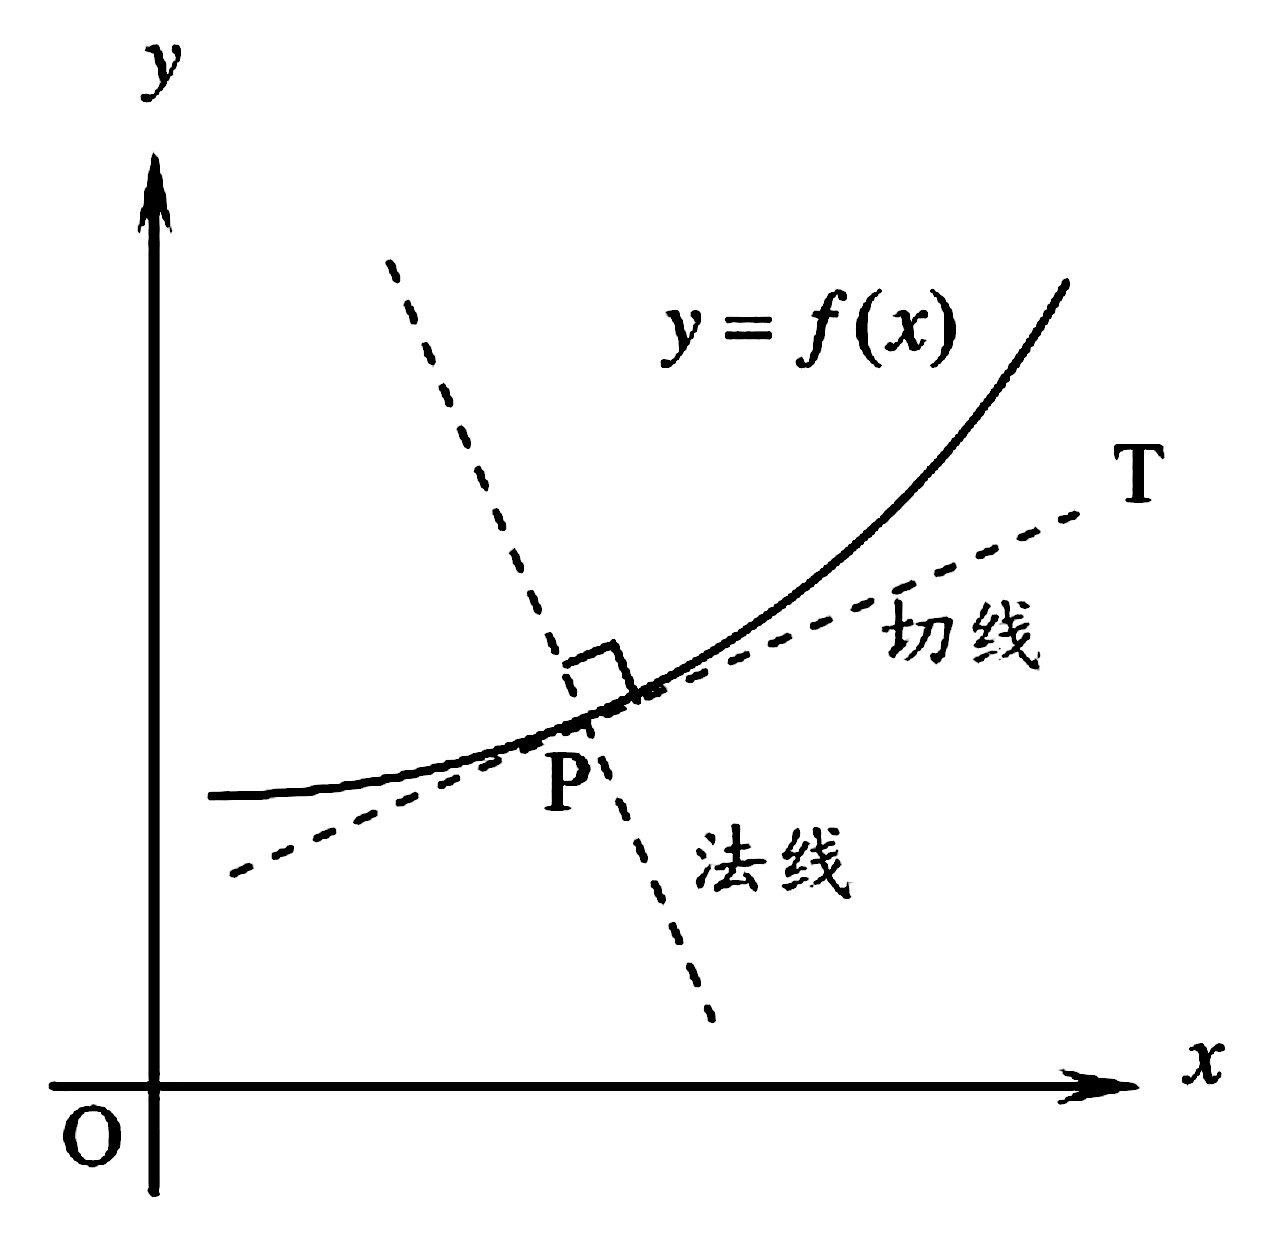
\includegraphics[scale=0.25]{assets/26-1.png}
    \end{center}
\end{multicols}

\subsection{Practice 1}
\begin{enumerate}
      \item Find the equations of tangent and normal to the curve $y = x^3$ where $x = 2$.
            \sol{} \vspace{-1cm}
            \begin{multicols}{2}
                  \begin{flalign*}
                        y              & = x^3  & \\
                        \dfrac{dy}{dx} & = 3x^2
                  \end{flalign*}
                  At $x = 2$, $y = (2)^3 = 8$
                  \begin{flalign*}
                        \text{Gradient of tangent } \dfrac{dy}{dx} & = 3(2)^2 = 12    & \\
                        \text{Gradient of normal }                 & = -\dfrac{1}{12}
                  \end{flalign*}
                  \vfill\null
                  \begin{flalign*}
                        \therefore\ \text{Equation of tangent is } y - 8 & = 12(x - 2)             & \\
                        y                                                & = 12x - 16              & \\
                        \text{Equation of normal is } y - 8              & = -\dfrac{1}{12}(x - 2) & \\
                        12y - 96                                         & = -x + 2                & \\
                        x + 12y                                          & = 98                    & \\
                  \end{flalign*}
                  \vfill\null
            \end{multicols}
            \vspace{-1cm}

      \item Given that the gradient of tangent to the curve $y = x^2 - 2x + 3$ at point $Q$
            is $4$, find the coordinates of the point $Q$. \sol{}
            \begin{flalign*}
                  y              & = x^2 - 2x + 3 & \\
                  \dfrac{dy}{dx} & = 2x - 2
            \end{flalign*}
            At point $Q$, $\dfrac{dy}{dx} = 4$
            \begin{flalign*}
                  4 & = 2x - 2             & \\
                  x & = 3                  & \\
                  y & = 3^2 - 2(3) + 3 = 6
            \end{flalign*}
            $\therefore$ Coordinates of point $Q$ is $(3, 6)$.
            \vfill\null

      \item Find the equations of the tangent and normal to the curve $x^3 - 2xy + y^2 = 1$
            at point $(1, 2)$. \sol{}
            \begin{flalign*}
                  x^3 - 2xy + y^2                                 & = 1                          & \\
                  3x^2 - 2y - 2x\dfrac{dy}{dx} + 2y\dfrac{dy}{dx} & = 0                          & \\
                  (2x - 2y) \dfrac{dy}{dx}                        & = 3x^2 - 2y                  & \\
                  \dfrac{dy}{dx}                                  & = \dfrac{3x^2 - 2y}{2x - 2y}
            \end{flalign*}
            At point $(1, 2)$,
            \begin{flalign*}
                  \text{Gradient of tangent } \dfrac{dy}{dx} & = \dfrac{3(1)^2 - 2(2)}{2(1) - 2(2)} & \\
                                                             & = \dfrac{1}{2}                       & \\
                  \text{Gradient of normal }                 & = -2
            \end{flalign*}
            \begin{flalign*}
                  \therefore\ \text{Equation of tangent is } y - 2 & = \dfrac{1}{2}(x - 1) & \\
                  2y - 4                                           & = x - 1               & \\
                  x - 2y                                           & = -3                  & \\
                  \text{Equation of normal is } y - 2              & = -2(x - 1)           & \\
                  y - 2                                            & = -2x + 2             & \\
                  y                                                & = -2x + 4
            \end{flalign*}
            \vfill\null
\end{enumerate}
\newpage
\subsection{Exercise 26.1}
\begin{enumerate}
      \begin{multicols}{2}
            \item Find the equations of the tangent and normal to the curve $y = x^2 + 2$ at
            point $(2, 6)$. \sol{}
            \begin{flalign*}
                  y              & = x^2 + 2 & \\
                  \dfrac{dy}{dx} & = 2x
            \end{flalign*}
            At point $(2, 6)$,
            \begin{flalign*}
                  \text{Gradient of tangent } \dfrac{dy}{dx} & = 2(2) = 4      & \\
                  \text{Gradient of normal }                 & = -\dfrac{1}{4}
            \end{flalign*}
            \begin{flalign*}
                  \therefore\ \text{Equation of tangent is } y - 6 & = 4(x - 2)             & \\
                  y                                                & = 4x - 2               & \\
                  \text{Equation of normal is } y - 6              & = -\dfrac{1}{4}(x - 2) & \\
                  4y - 24                                          & = -x + 2               & \\
                  x + 4y                                           & = 26
            \end{flalign*}

            \item Find the equation of the tangent to the curve $y = 2x^3 - 3x^2 - 12x + 8$ where
            $x = 0$. \sol{}
            \begin{flalign*}
                  y              & = 2x^3 - 3x^2 - 12x + 8 & \\
                  \dfrac{dy}{dx} & = 6x^2 - 6x - 12
            \end{flalign*}
            At $x = 0$, $y = 8$
            \begin{flalign*}
                  \text{Gradient of tangent } \dfrac{dy}{dx}       & = 6(0)^2 - 6(0) - 12 = -12 & \\
                  \therefore\ \text{Equation of tangent is } y - 8 & = -12(x - 0)               & \\
                  y                                                & = -12x + 8
            \end{flalign*}
      \end{multicols}
      \vfill\null

      \begin{multicols}{2}
            \item Find the equation of the normal to the curve $y = 3x^3 - 4x + 7$ at point $(1,
                  6)$. \sol{}
            \begin{flalign*}
                  y              & = 3x^3 - 4x + 7 & \\
                  \dfrac{dy}{dx} & = 9x^2 - 4
            \end{flalign*}
            At point $(1, 6)$,
            \begin{flalign*}
                  \text{Gradient of tangent } \dfrac{dy}{dx} & = 9(1)^2 - 4 = 5 & \\
                  \text{Gradient of normal }                 & = -\dfrac{1}{5}
            \end{flalign*}
            \begin{flalign*}
                  \therefore\ \text{Equation of normal is } y - 6 & = -\dfrac{1}{5}(x - 1) & \\
                  5y - 30                                         & = -x + 1               & \\
                  x + 5y                                          & = 31
            \end{flalign*}

            \item Find the equation of the tangent to the curve $y = \dfrac{1}{1-x}$ where $x =
                  -1$. \sol{}
            \begin{flalign*}
                  y              & = \dfrac{1}{1-x}     & \\
                  \dfrac{dy}{dx} & = \dfrac{1}{(1-x)^2}
            \end{flalign*}
            At $x = -1$, $y = \dfrac{1}{2}$
            \begin{flalign*}
                  \text{Gradient of tangent } \dfrac{dy}{dx}                  & = \dfrac{1}{[1-(-1)]^2} = \dfrac{1}{4} & \\
                  \therefore\ \text{Equation of tangent is } y - \dfrac{1}{2} & = \dfrac{1}{4}(x + 1)                  & \\
                  4y - 2                                                      & = x+1                                  & \\
                  x - 4y + 3                                                  & = 0
            \end{flalign*}
      \end{multicols}
      \vfill\null

      \newpage
      \item Find the equations of the tangent and normal to the curve $y = 1 - 2x^2$ where
            $x = -2$. \sol{}
            \begin{flalign*}
                  y              & = 1 - 2x^2 & \\
                  \dfrac{dy}{dx} & = -4x
            \end{flalign*}
            At $x = -2$, $y = 1 - 2(-2)^2 = -7$
            \begin{flalign*}
                  \text{Gradient of tangent } \dfrac{dy}{dx} & = -4(-2) = 8    & \\
                  \text{Gradient of normal }                 & = -\dfrac{1}{8}
            \end{flalign*}
            \begin{flalign*}
                  \therefore\ \text{Equation of tangent is } y + 7 & = 8(x + 2)             & \\
                  y                                                & = 8x + 9               & \\
                  \text{Equation of normal is } y + 7              & = -\dfrac{1}{8}(x + 2) & \\
                  8y + 56                                          & = -x - 2               & \\
                  x + 8y + 58                                      & = 0
            \end{flalign*}

      \item Find the equation of the tangent to the curve $y = (x+1)(x-1)(x-3)$ where the
            curve intersects with the $x$-axis. \sol{}
            \begin{flalign*}
                  y              & = (x+1)(x-1)(x-3)    & \\
                                 & = (x^2 - 1)(x-3)     & \\
                                 & = x^3 - 3x^2 - x + 3 & \\
                  \dfrac{dy}{dx} & = 3x^2 - 6x - 1
            \end{flalign*}
            At $y = 0$, $x = -1, 1, 3$.

            When $x = -1$,
            \begin{flalign*}
                  \text{Gradient of tangent } \dfrac{dy}{dx}   & = 3(-1)^2 - 6(-1) - 1 = 8 & \\
                  \therefore\ \text{Equation of tangent is } y & = 8(x + 1)                & \\
                  y                                            & = 8x + 8
            \end{flalign*}
            When $x = 1$,
            \begin{flalign*}
                  \text{Gradient of tangent } \dfrac{dy}{dx}   & = 3(1)^2 - 6(1) - 1 = -4 & \\
                  \therefore\ \text{Equation of tangent is } y & = -4(x - 1)              & \\
                  y                                            & = -4x + 4
            \end{flalign*}
            When $x = 3$,
            \begin{flalign*}
                  \text{Gradient of tangent } \dfrac{dy}{dx}   & = 3(3)^2 - 6(3) - 1 = 8 & \\
                  \therefore\ \text{Equation of tangent is } y & = 8(x - 3)              & \\
                  y                                            & = 8x - 24
            \end{flalign*}

      \item Find the equation of the tangent to the curve $y = 4x^3 - 27x + 7$ that is
            parallel to the $x$-axis. \sol{}
            \begin{flalign*}
                  y              & = 4x^3 - 27x + 7 & \\
                  \dfrac{dy}{dx} & = 12x^2 - 27
            \end{flalign*}
            The tangent is parallel to the $x$-axis when $\dfrac{dy}{dx} = 0$.
            \begin{flalign*}
                  12x^2 - 27 & = 0               & \\
                  4x^2       & = 9               & \\
                  x          & = \pm\dfrac{3}{2}
            \end{flalign*}
            When $x = \dfrac{3}{2}$, $y = 4\left(\dfrac{3}{2}\right)^3 - 27\left(\dfrac{3}{2}\right) + 7 = -20$
            \begin{flalign*}
                  \therefore\ \text{Equation of tangent is } y + 20 & = 0(x - \dfrac{3}{2}) & \\
                  y                                                 & = -20
            \end{flalign*}

            When $x = -\dfrac{3}{2}$, $y = 4\left(-\dfrac{3}{2}\right)^3 -
                  27\left(-\dfrac{3}{2}\right) + 7 = 34$
            \begin{flalign*}
                  \therefore\ \text{Equation of tangent is } y - 34 & = 0(x + \dfrac{3}{2}) & \\
                  y                                                 & = 34
            \end{flalign*}

      \item Find the equation of the tangent to the curve $y = 11x - 3x^2$ that is parallel
            to the line $x + y - 2 = 0$. \sol{}
            \begin{flalign*}
                  x + y - 2 & = 0      & \\
                  y         & = -x + 2
            \end{flalign*}
            The gradient of the line $x + y - 2 = 0$ is $-1$.
            \begin{flalign*}
                  y              & = 11x - 3x^2 & \\
                  \dfrac{dy}{dx} & = 11 - 6x
            \end{flalign*}
            The tangent is parallel to the line $x + y - 2 = 0$ when $\dfrac{dy}{dx} = -1$.
            \begin{flalign*}
                  11 - 6x & = -1 & \\
                  6x      & = 12 & \\
                  x       & = 2
            \end{flalign*}
            When $x = 2$, $y = 11(2) - 3(2)^2 = 10$
            \begin{flalign*}
                  \therefore\ \text{Equation of tangent is } y - 10 & = -1(x - 2) & \\
                  y                                                 & = -x + 12
            \end{flalign*}
            \begin{multicols}{2}
                  \item Find the equations of the tangent and normal to the curve $y = \ln{(2x - 1)}$
                  where $x=1$. \sol{}
                  \begin{flalign*}
                        y              & = \ln{(2x - 1)}     & \\
                        \dfrac{dy}{dx} & = \dfrac{2}{2x - 1}
                  \end{flalign*}
                  At $x = 1$, $y = \ln{(2(1) - 1)} = \ln{1} = 0$
                  \begin{flalign*}
                        \text{Gradient of tangent } \dfrac{dy}{dx} & = \dfrac{2}{2(1) - 1} = 2 & \\
                        \text{Gradient of normal }                 & = -\dfrac{1}{2}
                  \end{flalign*}
                  \begin{flalign*}
                        \therefore\ \text{Equation of tangent is } y - 0 & = 2(x - 1)             & \\
                        y                                                & = 2x - 2               & \\
                        \text{Equation of normal is } y - 0              & = -\dfrac{1}{2}(x - 1) & \\
                        2y                                               & = -x + 1               & \\
                        x + 2y                                           & = 1
                  \end{flalign*}
                  \item If the straight line $y = 8x + k$ is the tangent to the curve $y = x^2 + 4x -
                        3$, find the value of $k$. \sol{}

                  The gradient of the tangent line is $8$.
                  \begin{flalign*}
                        y              & = x^2 + 4x - 3 & \\
                        \dfrac{dy}{dx} & = 2x + 4       & \\
                        8              & = 2x + 4       & \\
                        x              & = 2
                  \end{flalign*}
                  When $x = 2$, $y = 2^2 + 4(2) - 3 = 9$

                  Substituting $x = 2$ and $y = 9$ into $y = 8x + k$,
                  \begin{flalign*}
                        9 & = 8(2) + k & \\
                        k & = -7
                  \end{flalign*}
            \end{multicols}

            \begin{multicols}{2}
                  \item Given that the gradient of tangent to the curve $y = ax + bx^2$ at point $(1,
                        0)$ is $\dfrac{1}{2}$, find the value of $a$ and $b$. \sol{}
                  \begin{flalign*}
                        y              & = ax + bx^2 & \\
                        \dfrac{dy}{dx} & = a + 2bx
                  \end{flalign*}
                  At point $(1, 0)$,
                  \begin{flalign*}
                        a(1) + b(1)^2                              & = 0                         & \\
                        a + b                                      & = 0\ \cdots\ (1)            & \\
                        \text{Gradient of tangent } \dfrac{dy}{dx} & = a + 2b(1) = \dfrac{1}{2}  & \\
                        a + 2b                                     & = \dfrac{1}{2}\ \cdots\ (2)
                  \end{flalign*}
                  Solving $(1)$ and $(2)$, $b = \dfrac{1}{2}$ and $a = -\dfrac{1}{2}$.
                  \vfill\null

                  \item If $x + y + 2 = 0$ is the equation of tangent to the curve $y = ax^2 + bx$
                  where $x = 1$, find the value of $a$ and $b$. \sol{}
                  \begin{flalign*}
                        x + y + 2 & = 0      & \\
                        y         & = -x - 2
                  \end{flalign*}
                  The gradient of the tangent line is $-1$.
                  \begin{flalign*}
                        y              & = ax^2 + bx & \\
                        \dfrac{dy}{dx} & = 2ax + b
                  \end{flalign*}
                  At $x = 1$, $y = -1 - 2 = -3$
                  \begin{flalign*}
                        -3                                         & = a(1)^2 + b(1)   & \\
                        a + b                                      & = -3\ \cdots\ (1) & \\
                        \text{Gradient of tangent } \dfrac{dy}{dx} & = 2a(1) + b = -1  & \\
                        2a + b                                     & = -1\ \cdots\ (2)
                  \end{flalign*}
                  Solving $(1)$ and $(2)$, $a = 2$ and $b = -5$.
            \end{multicols}

            \newpage
            \begin{multicols}{2}
                  \item Given that the gradient of tangent to the curve $y = x^3 - 6x^2 + 10x - 5$ at
                  point $P$ is $-2$, find the coordinates of $P$. \sol{}
                  \begin{flalign*}
                        y              & = x^3 - 6x^2 + 10x - 5 & \\
                        \dfrac{dy}{dx} & = 3x^2 - 12x + 10
                  \end{flalign*}
                  At point $P$, $\dfrac{dy}{dx} = -2$
                  \begin{flalign*}
                        -2              & = 3x^2 - 12x + 10 & \\
                        3x^2 - 12x + 12 & = 0               & \\
                        x^2 - 4x + 4    & = 0               & \\
                        (x - 2)^2       & = 0               & \\
                        x               & = 2
                  \end{flalign*}
                  When $x = 2$, $y = 2^3 - 6(2)^2 + 10(2) - 5 = -1$

                  $\therefore$ Coordinates of point $P$ is $(2, -1)$.
                  \vfill\null

                  \item Prove that the tangent lines to the curve $y = x^2 - 3x + 1$ and the curve
                  $x(y+3) = 4$ at point $(2, -1)$ are perpendicular to each other. \prooff{}
                  \begin{flalign*}
                        y              & = x^2 - 3x + 1 & \\
                        \dfrac{dy}{dx} & = 2x - 3
                  \end{flalign*}
                  At point $(2, -1)$,
                  \begin{flalign*}
                        \text{Gradient of tangent } \dfrac{dy}{dx} & = 2(2) - 3 = 1
                  \end{flalign*}
                  \begin{flalign*}
                        x(y+3)         & = 4                & \\
                        y              & = \dfrac{4}{x} - 3 & \\
                        \dfrac{dy}{dx} & = -\dfrac{4}{x^2}
                  \end{flalign*}
                  At point $(2, -1)$,
                  \begin{flalign*}
                        \text{Gradient of tangent } \dfrac{dy}{dx} & = -\dfrac{4}{(2)^2} = -1
                  \end{flalign*}
                  Since the product of the gradients of the two lines is $1 \times -1 = -1$, the two lines are perpendicular to each other. \qed
            \end{multicols}

            \begin{multicols}{2}
                  \item Find the equations of the tangent and normal to the curve $x^2 - xy + y^2 = 7$
                  at point $(-2, -3)$. \sol{}
                  \begin{flalign*}
                        x^2 - xy + y^2                              & = 7                      & \\
                        2x - y - x\dfrac{dy}{dx} + 2y\dfrac{dy}{dx} & = 0                      & \\
                        (2y - x) \dfrac{dy}{dx}                     & = y - 2x                 & \\
                        \dfrac{dy}{dx}                              & = \dfrac{y - 2x}{2y - x}
                  \end{flalign*}
                  At point $(-2, -3)$,
                  \begin{flalign*}
                        \text{Gradient of tangent } \dfrac{dy}{dx} & = \dfrac{-3 - 2(-2)}{2(-3) - (-2)} = -\dfrac{1}{4} & \\
                        \text{Gradient of normal }                 & = 4
                  \end{flalign*}
                  \vspace{-1cm}
                  \begin{flalign*}
                        \therefore\ \text{Equation of tangent is } y + 3 & = -\dfrac{1}{4}(x + 2) & \\
                        4y + 12                                          & = -x - 2               & \\
                        x + 4y + 14                                      & = 0                    & \\
                        \text{Equation of normal is } y + 3              & = 4(x + 2)             & \\
                        y                                                & = 4x + 5
                  \end{flalign*}

                  \item Find the equation of tangent to the curve $y^2 + y = 2\sin x$ at point $(0,
                        -1)$.
                  \begin{flalign*}
                        y^2 + y = 2\sin x                           & \\
                        2y\dfrac{dy}{dx} + \dfrac{dy}{dx} = 2\cos x & \\
                        (2y + 1) \dfrac{dy}{dx} = 2\cos x           & \\
                        \dfrac{dy}{dx} = \dfrac{2\cos x}{2y + 1}
                  \end{flalign*}
                  At point $(0, -1)$,
                  \begin{flalign*}
                        \text{Gradient of tangent } \dfrac{dy}{dx}       & = \dfrac{2\cos 0}{2(-1) + 1} = -2 & \\
                        \therefore\ \text{Equation of tangent is } y + 1 & = -2(x - 0)                       & \\
                        y                                                & = -2x - 1
                  \end{flalign*}
            \end{multicols}
\end{enumerate}

\newpage

\section{Increasing and Decreasing Functions}

\subsection*{Monotonic Functions}

For a function $f(x)$ being defined in the interval $D$,
\begin{enumerate}
    \item For any two numbers $x_1$ and $x_2$ in $D$, when $x_1 < x_2$, $f(x)$ is an
          increasing function in the interval $D$, as shown in the figure below.
          \begin{center}
              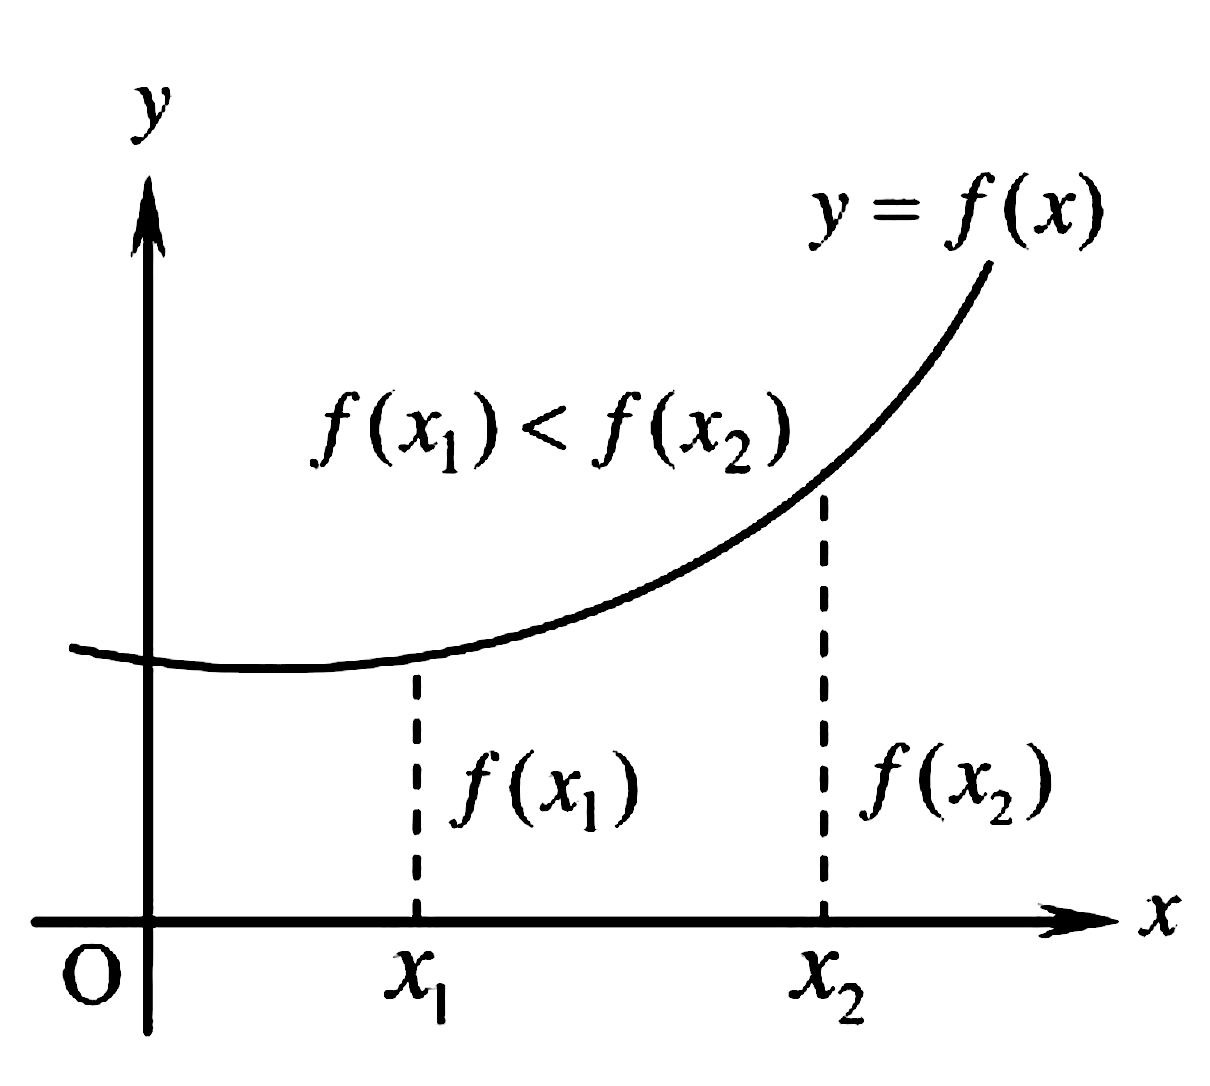
\includegraphics[scale=0.25]{assets/26-2.png}
          \end{center}
    \item For any two numbers $x_1$ and $x_2$ in $D$, when $x_1 > x_2$, $f(x)$ is a
          decreasing function in the interval $D$, as shown in the figure below.
          \begin{center}
              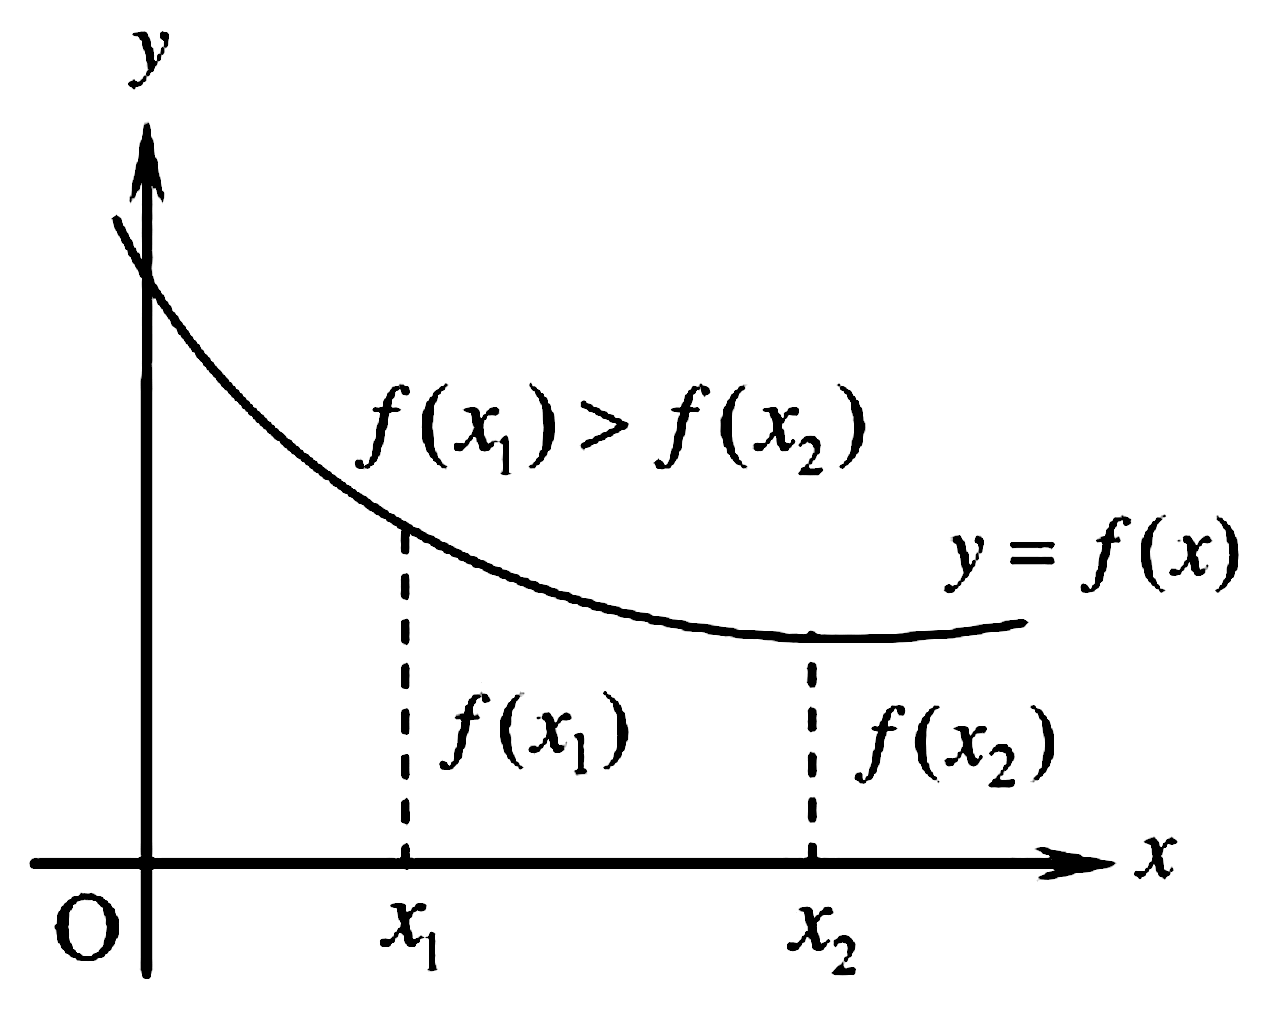
\includegraphics[scale=0.25]{assets/26-3.png}
          \end{center}
\end{enumerate}
If $f(x)$ is an increasing function or a decreasing function in the interval $D$, we call $f(x)$ a monotonic function in the interval $D$.
\begin{center}
    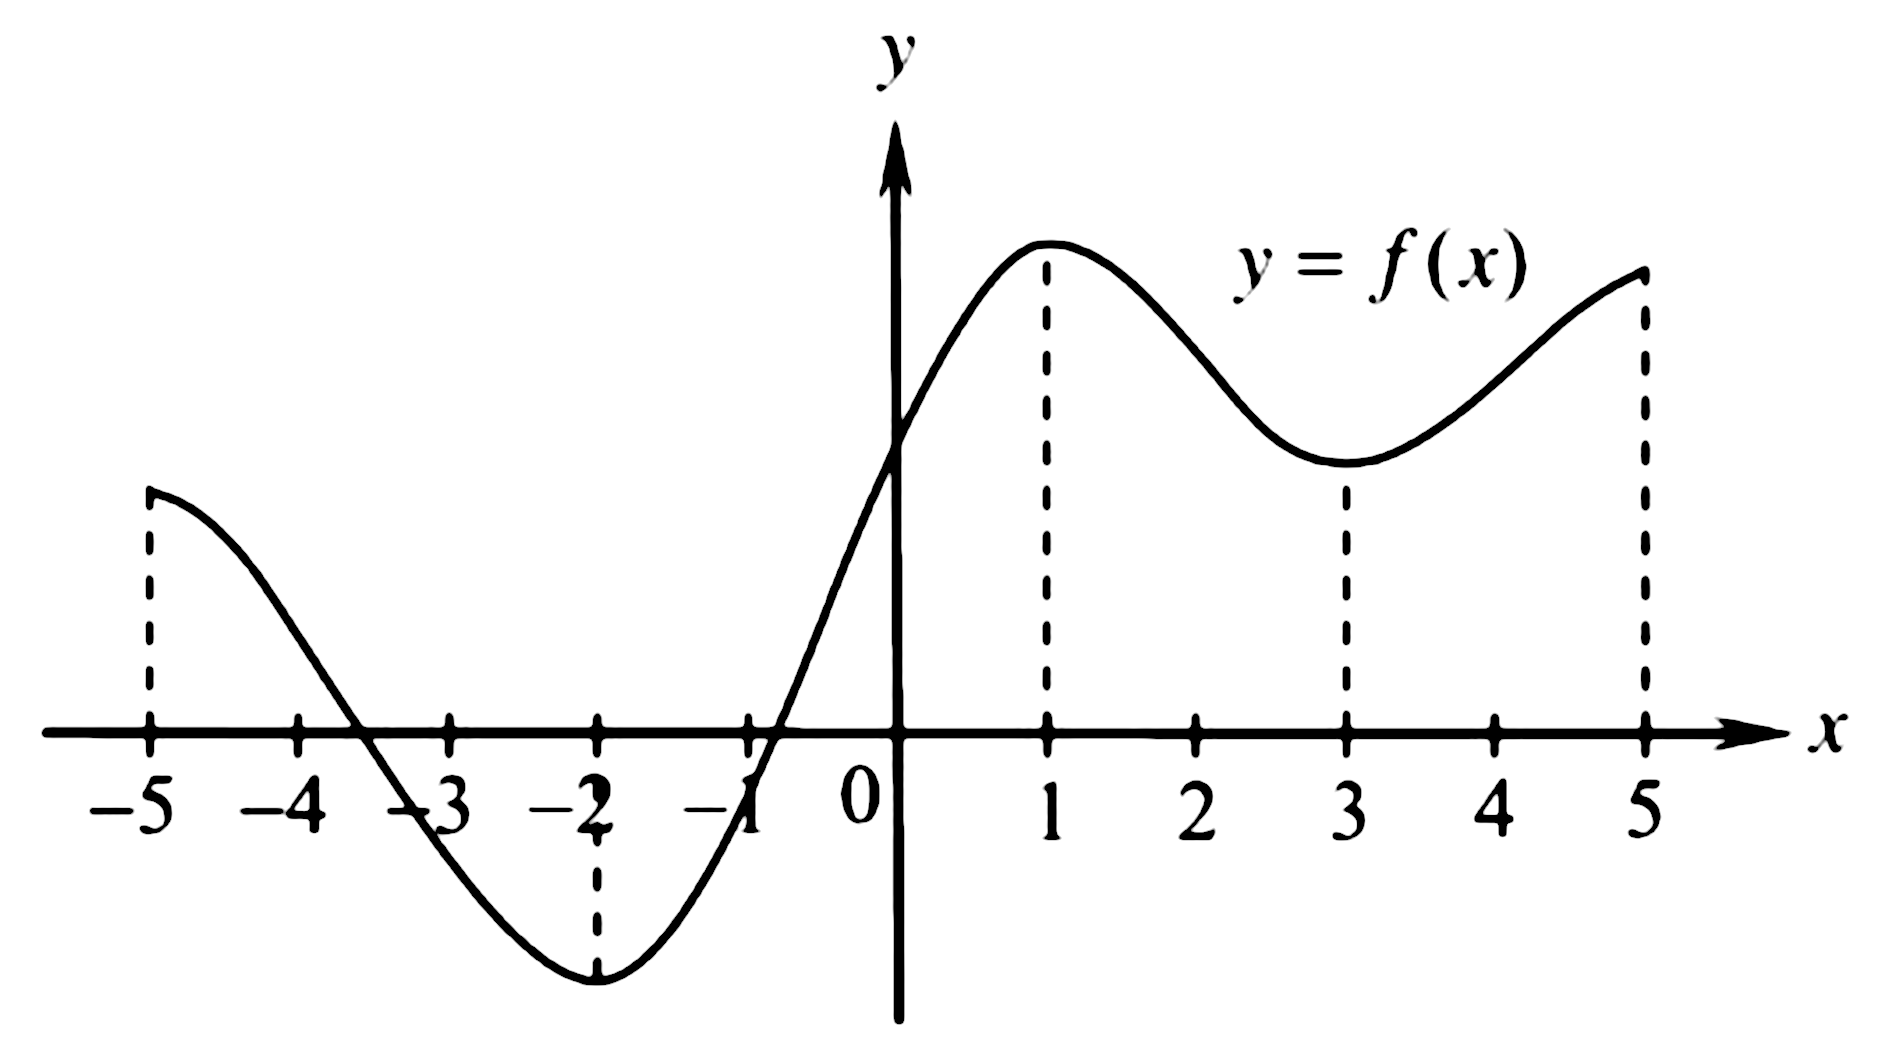
\includegraphics[scale=0.25]{assets/26-4.png}
\end{center}
The curve shown in the diagram above is the graph of the function $f(x)$ in the
interval $[-5, 5]$. From the graph, we can see that the function $f(x)$ is a
decreasing function in the intervals $[-5, 2]$ and $[1, 3]$, and an increasing
function in the interval $[-2, 1]$ and $[3, 5]$.
\newpage

\subsection*{How to Judge the Increase or Decrease of Functions}

As shown in the diagram below, when the function $f(x)$ is an increasing
function in the interval $[a, b]$, the gradient of the tangent to the curve at
any point in the interval $(a, b)$ is positive, i.e. $f'(x) > 0$; when the
function $f(x)$ is a decreasing function in the interval $[b, c]$, the gradient
of the tangent to the curve at any point in the interval $(b, c)$ is negative,
i.e. $f'(x) < 0$.
\begin{center}
    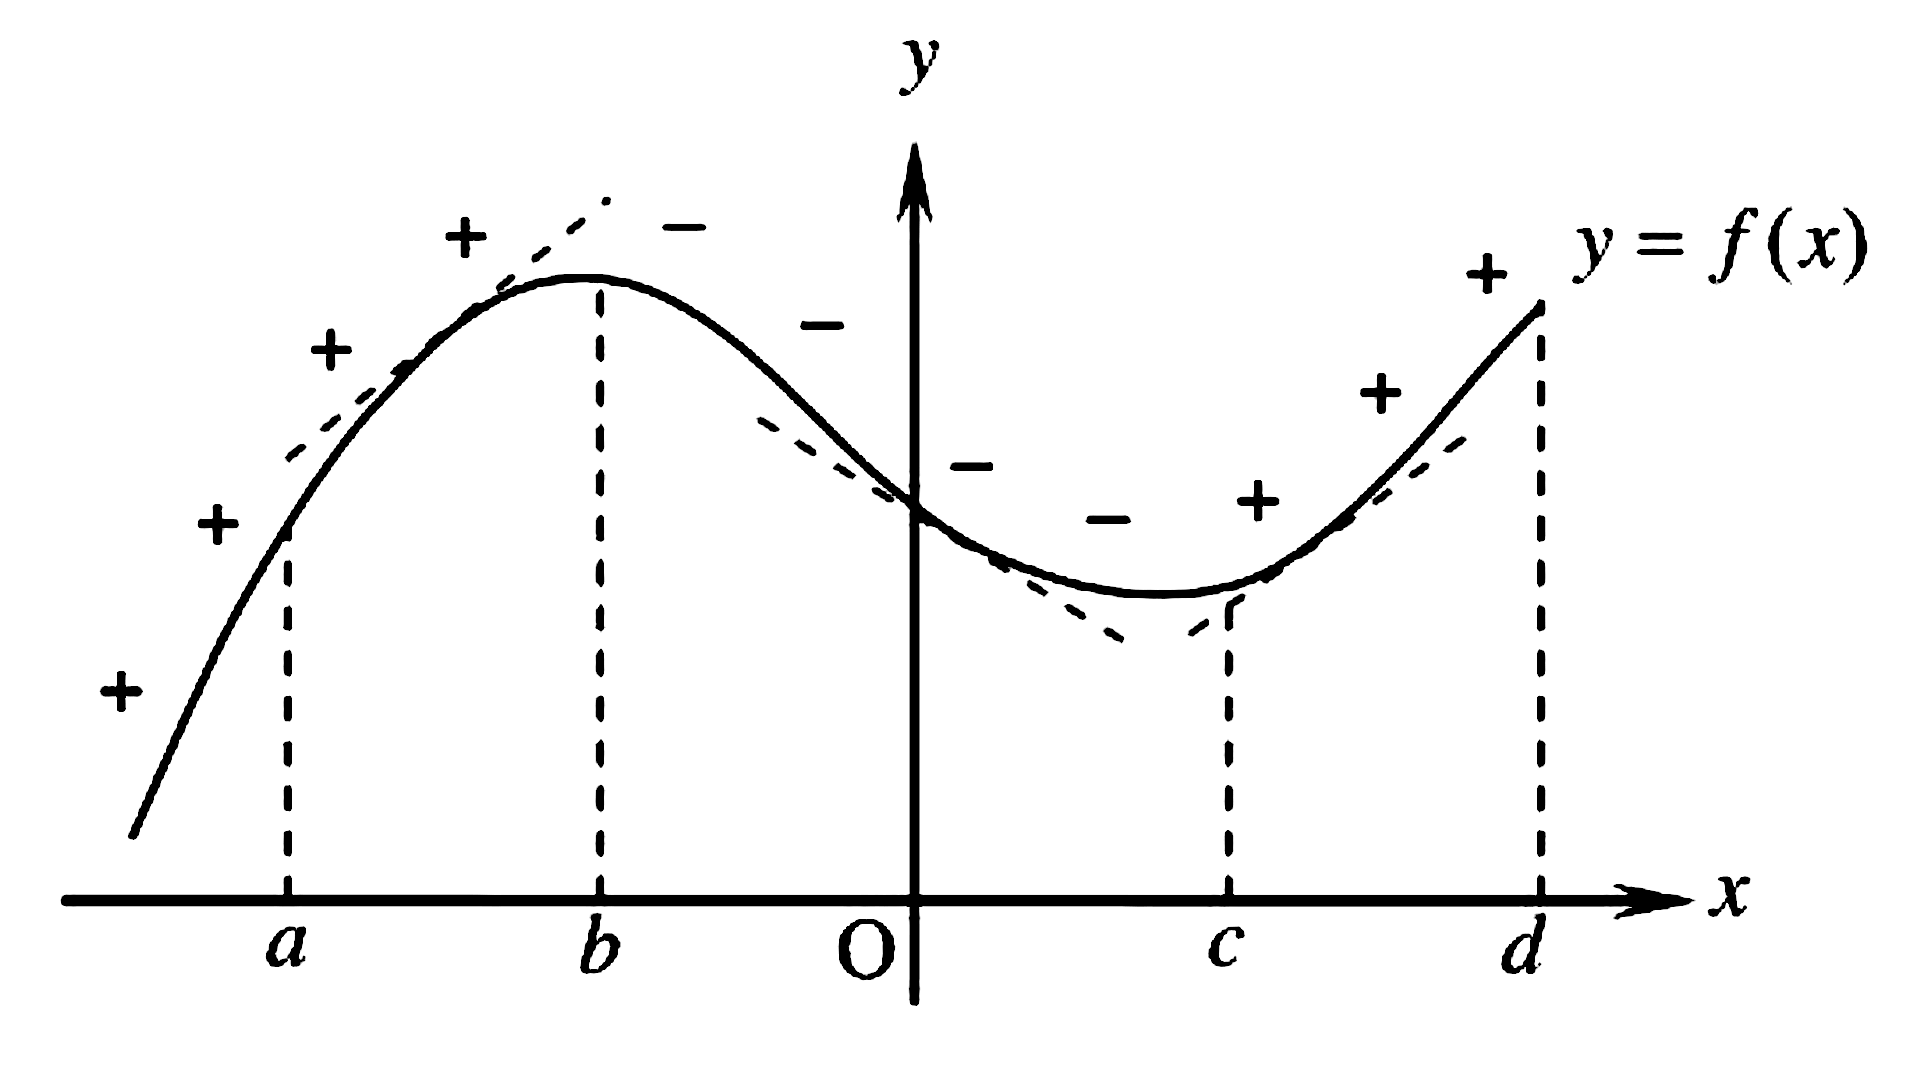
\includegraphics[scale=0.25]{assets/26-5.png}
\end{center}
Therefore, we can judge whether a function is an increasing function or a decreasing function in an interval by the sign of the derivative value of the function in the interval:
\begin{center}
    \framebox{
        \parbox[t][3.8cm]{14cm}{ \addvspace{0.6cm} \hspace{0.4cm}Let $f(x)$ be a continuous
            function defined in the interval $[a, b]$, and can be differentiated in

            \hspace{0.4cm}the interval $(a, b)$.

            \begin{itemize}[leftmargin=0.76cm]
                \item In the interval $(a, b)$, if $f'(x) > 0$, then $f(x)$ is an increasing function
                      in the interval $[a, b]$.
                \item In the interval $(a, b)$, if $f'(x) < 0$, then $f(x)$ is a decreasing function
                      in the interval $[a, b]$.
            \end{itemize} }}
\end{center}
\vspace{0.9em}

\subsection{Practice 2}

\begin{enumerate}
    \begin{multicols}{2}
        \item $\displaystyle\int_2^8 x d x$
        \sol{}
        \begin{flalign*}
            I & = \left[\dfrac{1}{2}x^2\right]_2^8 & \\
              & = \dfrac{1}{2}(64 - 4)             & \\
              & = 30
        \end{flalign*}

        \item $\displaystyle\int_{-2}^4 x^3 d x$
        \sol{}
        \begin{flalign*}
            I & = \left[\dfrac{1}{4}x^4\right]_{-2}^4 & \\
              & = \dfrac{1}{4}(256 - 16)              & \\
              & = 60
        \end{flalign*}
    \end{multicols}
    \begin{multicols}{2}
        \item $\displaystyle\int_{-\pi}^\pi \cos x d x$
        \sol{}
        \begin{flalign*}
            I & = \bigg[\sin x\bigg]_{-\pi}^\pi & \\
              & = \sin\pi - \sin(-\pi)          & \\
              & = 0 - 0                         & \\
              & = 0
        \end{flalign*}

        \item $\displaystyle\int_0^{\frac{\pi}{4}} \sec ^2 x d x$
        \sol{}
        \begin{flalign*}
            I & = \bigg[\tan x\bigg]_0^{\frac{\pi}{4}} & \\
              & = \tan\dfrac{\pi}{4} - \tan 0          & \\
              & = 1 - 0                                & \\
              & = 1
        \end{flalign*}
    \end{multicols}
\end{enumerate}
\subsection{Exercise 26.2}

\noindent \hspace{1.2em}\textit{Determine which intervals the following functions is an increasing function or a decreasing function.}
\begin{enumerate}
    \begin{multicols}{2}
        \item $f(x)=x^2-2 x+4$
        \sol{}
        \begin{flalign*}
            f'(x)  & = 2x - 2 & \\
            2x - 2 & = 0      & \\
            x      & = 1
        \end{flalign*}
        In the interval $(-\infty,1)$, $f'(x)<0$, so $f(x)$ is a decreasing function in the interval $(-\infty,1]$.

        In the interval $(1,\infty)$, $f'(x)>0$, so $f(x)$ is an increasing function in
        the interval $[1,\infty)$. \vfill\null

                        \item $f(x)=2 x^3-6 x^2+7$
                        \sol{}
                        \begin{flalign*}
                            f'(x)      & = 6x^2 - 12x          & \\
                            6x^2 - 12x & = 0                   & \\
                            x(x - 2)   & = 0                   & \\
                            x          & = 0 \text{ or } x = 2
                        \end{flalign*}
                        In the interval $(-\infty,0)$, $f'(x)>0$, so $f(x)$ is an increasing function in the interval $(-\infty,0]$.

        In the interval $(0,2)$, $f'(x)<0$, so $f(x)$ is a decreasing function in the
        interval $[0,2]$.

        In the interval $(2,\infty)$, $f'(x)>0$, so $f(x)$ is an increasing function in
        the interval $[2,\infty)$.
    \end{multicols}
    \vfill\null

    \begin{multicols}{2}
        \item $f(x)=x^3+x$
        \sol{}
        \begin{flalign*}
            f'(x)    & = 3x^2 + 1        & \\
            3x^2 + 1 & = 0               & \\
            x^2      & = -\frac{1}{3}      \\
            x        & \notin \mathbb{R}
        \end{flalign*}
        Since $f'(x)>0$ for all $x \in \mathbb{R}$, $f(x)$ is an increasing function.
        \vfill\null

        \item $f(x)=2+3 x-x^3$
        \sol{}
        \begin{flalign*}
            f'(x)    & = 3 - 3x^2 & \\
            3 - 3x^2 & = 0        & \\
            x^2      & = 1          \\
            x        & = \pm 1
        \end{flalign*}
        In the interval $(-\infty,-1)$, $f'(x)<0$, so $f(x)$ is a decreasing function in the interval $(-\infty,-1]$.

        In the interval $(-1,1)$, $f'(x)>0$, so $f(x)$ is an increasing function in the
        interval $[-1,1]$.

        In the interval $(1,\infty)$, $f'(x)<0$, so $f(x)$ is a decreasing function in
        the interval $[1,\infty)$.
    \end{multicols}
    \vfill\null
    \newpage

    \begin{multicols}{2}
        \item $f(x)=x^2(x-3)$
        \sol{}
        \begin{flalign*}
            f(x)      & = x^3 - 3x^2          & \\
            f'(x)     & = 3x^2 - 6x           & \\
            3x^2 - 6x & = 0                   & \\
            x(x - 2)  & = 0                   & \\
            x         & = 0 \text{ or } x = 2
        \end{flalign*}
        In the interval $(-\infty,0)$, $f'(x)>0$, so $f(x)$ is an increasing function in the interval $(-\infty,0]$.

        In the interval $(0,2)$, $f'(x)<0$, so $f(x)$ is a decreasing function in the
        interval $[0,2]$.

        In the interval $(2,\infty)$, $f'(x)>0$, so $f(x)$ is an increasing function in
        the interval $[2,\infty)$. \vfil\null

                        \item $f(x)=3 x^4+2 x^3-3 x^2-2$
                        \sol{}
                        \begin{flalign*}
                            f'(x)                    & = 12x^3 + 6x^2 - 6x         & \\
                            12x^3 + 6x^2             & = 6x                        & \\
                            x(2x^2 + x - 1)          & = 0                         & \\
                            x(x + 1)(2x - 1)         & = 0                         & \\
                            x = 0 \text{ or } x = -1 & \text{ or } x = \frac{1}{2}
                        \end{flalign*}
                        In the interval $(-\infty,-1)$, $f'(x)<0$, so $f(x)$ is a decreasing function in the interval $(-\infty,-1]$.

        In the interval $(-1,0)$, $f'(x)>0$, so $f(x)$ is an increasing function in the
        interval $[-1,0]$.

        In the interval $(0,\frac{1}{2})$, $f'(x)<0$, so $f(x)$ is a decreasing
        function in the interval $[0,\frac{1}{2}]$.

        In the interval $(\frac{1}{2},\infty)$, $f'(x)>0$, so $f(x)$ is an increasing
        function in the interval $[\frac{1}{2},\infty)$.
    \end{multicols}
    \vfill\null

    \begin{multicols}{2}
        \item $f(x)=\dfrac{x}{x^2+1}$
        \sol{}
        \begin{flalign*}
            f'(x)   & = \frac{(x^2+1) - x(2x)}{(x^2+1)^2} & \\
                    & = \frac{1 - x^2}{(x^2+1)^2}         & \\
            1 - x^2 & = 0                                 & \\
            x^2     & = 1                                 & \\
            x       & = \pm 1
        \end{flalign*}
        In the interval $(-\infty,-1)$, $f'(x) < 0$, so $f(x)$ is a decreasing function in the interval $(-\infty,-1]$.

        In the interval $(-1,1)$, $f'(x) > 0$, so $f(x)$ is an increasing function in
        the interval $[-1,1]$.

        In the interval $(1,\infty)$, $f'(x) < 0$, so $f(x)$ is a decreasing function
        in the interval $[1,\infty)$.\columnbreak

        \item $f(x)=\cos 2 x, 0 \leq x \leq \pi$
        \sol{}
        \begin{flalign*}
            f'(x)      & = -2 \sin 2x                       & \\
            -2 \sin 2x & = 0                                & \\
            \sin 2x    & = 0                                & \\
            2x         & = \sin^{-1} 0                      & \\
            x          & = 0 \text{ or } x = \dfrac{\pi}{2}
        \end{flalign*}
        In the interval $\left[0,\dfrac{\pi}{2}\right]$, $f'(x) < 0$, so $f(x)$ is a decreasing function in the interval $\left[0,\dfrac{\pi}{2}\right]$.

        In the interval $\left[\dfrac{\pi}{2},\pi\right]$, $f'(x) > 0$, so $f(x)$ is an
        increasing function in the interval $\left[\dfrac{\pi}{2},\pi\right]$.
    \end{multicols}
    \vfill\null
\end{enumerate}

\section{Relative Maximum and Minimum Values of Functions}

As shown in the diagram below, the function value $f(a)$ at the point where
$x=a$ is the maximum compared to its nearby points, we call $f(a)$ the relative
maximum value; the function value $f(b)$ at the point where $x=b$ is the
minimum compared to its nearby points, we call $f(b)$ the relative minimum
value.
\begin{center}
    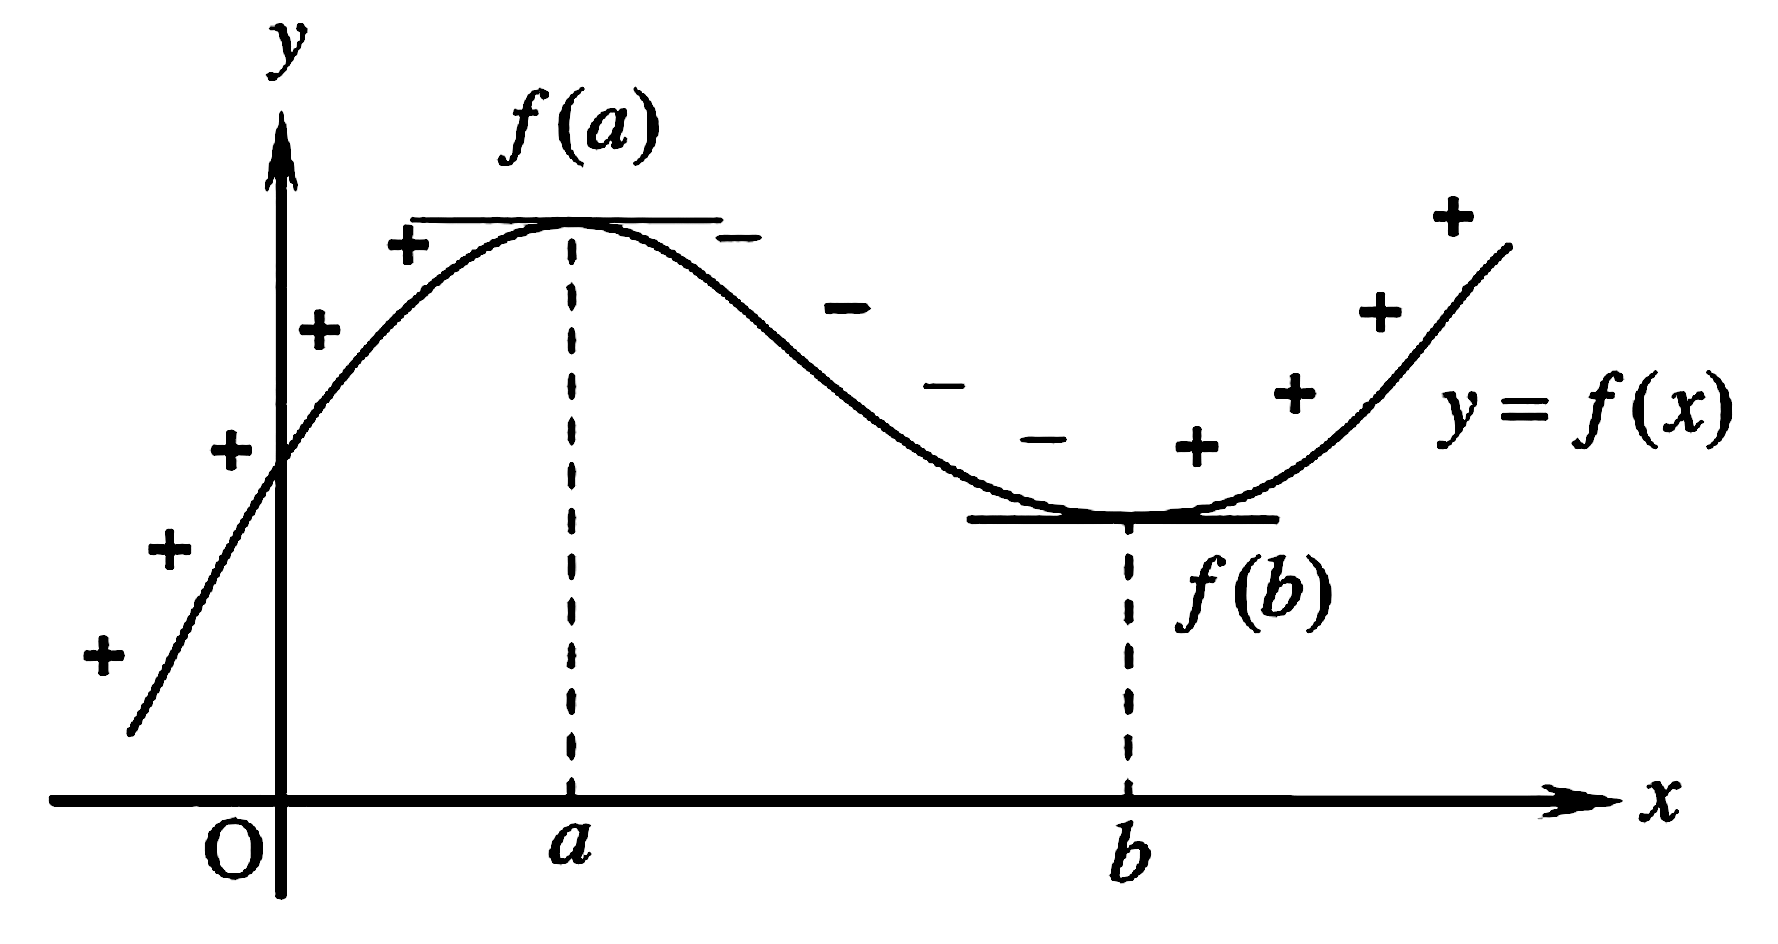
\includegraphics[scale=0.25]{assets/26-6.png}
\end{center}

\begin{center}
    \framebox{
        \parbox[t][5cm]{14cm}{ \addvspace{0.6cm} \hspace{0.4cm}Let $f(x)$ be a defined
            function near point $x=a$,
            \begin{itemize}
                \item \parbox[t]{12.5cm}{If the function value $f(a)$ is the maximum compared to its
                          nearby points, we say that $f(x)$ has a relative maximum value $f(a)$ at point
                          $x=a$, and the point $(a, f(a))$ is the relative maximum point of the
                          function;}
                \item \parbox[t]{12.5cm}{If the function value $f(a)$ is the minimum compared to its
                          nearby points, we say that $f(x)$ has a relative minimum value $f(a)$ at point
                          $x=a$, and the point $(a, f(a))$ is the relative minimum point of the
                          function.}
            \end{itemize}
        }}
\end{center}
\vspace{0.9em}

Relative maximum and minimum values are collectively known as the extreme
values, and the points where the extreme values occur are collectively known as
the extreme points.

From the diagram above, we can also see that the gradients of the tangent to
the curve at the extreme points are zero. Hence, the following theorem can be
obtained:
\begin{center}
    \framebox{
        \parbox[t][1.6cm]{14cm}{ \addvspace{0.4cm} \centering \parbox{13cm}{If the function $f(x)$ is differentiable at point $x=a$, and $f(x)$
                has a relative maximum or minimum value at point $x=a$, then $f'(a)=0$.} }}
\end{center}

\begin{multicols}{2}
    The points that satisfy $f'(x)=0$ are called the stationary points of the
    function.

    If the function can be differentiated at point $x=a$, then the extreme point
    must be a stationary point. However, the stationary point is not necessarily an
    extreme point. For example, the derivative of the function $f(x)=x^3$ is
    $f'(x)=3x^2$, and $f'(0)=0$, i.e. $O(0, 0)$ is a stationary point of the
    function $f(x)=x^3$, but it is not an extreme point of the function, as shown
    in the right diagram. \vfill{}\null{}

    \columnbreak
    \begin{center}
        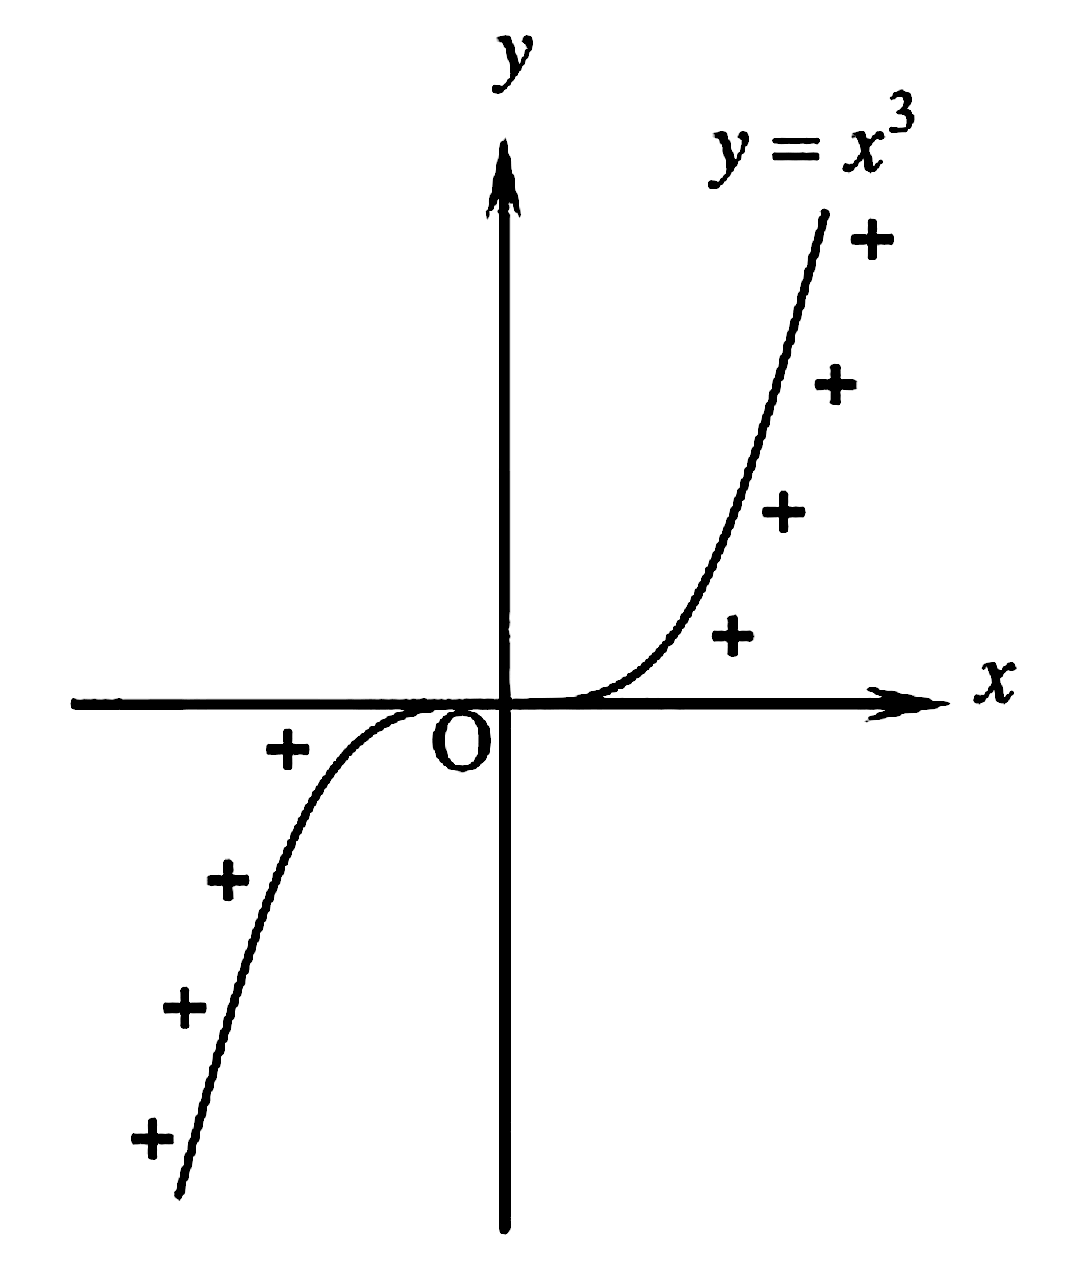
\includegraphics[scale=0.25]{assets/26-7.png}
    \end{center}
\end{multicols}

\subsection*{How to Find the Extreme Values of Functions}

\begin{enumerate}
    \item \textbf{First Derivative Test}

          The curve has a positive gradient of tangent to the left of the relative
          maximum point, and a negative gradient of tangent to the right; the curve has a
          negative gradient of tangent to the left of the relative minimum point, and a
          positive gradient of tangent to the right. Hence, the following theorem is
          obtained:
          \begin{center}
              \framebox{
                  \parbox[t][3.3cm]{14cm}{ \addvspace{0.4cm} \centering \parbox{13cm}{Let $f(x)$ be a function that is differentiable near point $x=a$, and
                          $f'(a) = 0$,
                          \begin{itemize}[leftmargin=0.4cm]
                              \item \parbox[t]{12.5cm}{If $f'(x) > 0$ to the left of $x=a$ and $f'(x) < 0$ to the right
                                        of $x=a$, then $f(a)$ is a relative maximum value;}
                              \item \parbox[t]{12.5cm}{If $f'(x) < 0$ to the left of $x=a$ and $f'(x) > 0$ to the right
                                        of $x=a$, then $f(a)$ is a relative minimum value.}
                          \end{itemize} }
                  }}
          \end{center}
          \vspace{0.9em}

    \item \textbf{Second Derivative Test}
          \begin{center}
              \framebox{
                  \parbox[t][2.5cm]{14cm}{ \addvspace{0.4cm} \centering \parbox{13cm}{Let $f(x)$ be a function that is second derivable near point $x=a$,
                          and $f'(a) = 0$,
                          \begin{itemize}[leftmargin=0.4cm]
                              \item \parbox[t]{12.5cm}{If $f''(a) < 0$, then $f(a)$ is a relative maximum value;}
                              \item \parbox[t]{12.5cm}{If $f''(a) > 0$, then $f(a)$ is a relative minimum value.}
                          \end{itemize} }
                  }}
          \end{center}

          Note that the second derivative test is invalid when $f''(a) = 0$, and the
          first derivative test should be used instead.
\end{enumerate}

\subsection{Practice 3}

\noindent \hspace{1.2em}\textit{
    Find the extreme values of the following functions (Question 1 to 4):
}

\begin{enumerate}
    \item $f(x)=x^2+x-6$
    \item $f(x)=2-x-x^2$
    \item $f(x)=\dfrac{1}{3} x^3-\dfrac{1}{2} x^2-2x+2$
    \item $f(x)=4 x-3 x^3$
\end{enumerate}

\noindent \hspace{1.2em}\textit{Find the coordinates of the extreme points of the following functions (Question 5 to 6):}
\begin{enumerate}[resume]
    \item $y=2 x^3-3 x^2-12 x-7$
    \item $y=x+\dfrac{1}{x}$
\end{enumerate}


\subsection{Exercise 26.3}

\noindent \hspace{1.2em}\textit{Find the extreme values of the following functions (Question 1 to 6):}
\begin{enumerate}
    \item $f(x)=\dfrac{1}{2} x^2-3 x$
    \item $f(x)=4+2 x-x^2$
    \item $f(x)=-2 x^2+4 x+7$
    \item $f(x)=3 x^2-2 x+1$
    \item $f(x)=2 x^3-9 x^2-24 x-12$
    \item $f(x)=15+9 x-3 x^2-x^3$
\end{enumerate}

\noindent \hspace{1.2em}\textit{Find the coordinates of the extreme points of the following functions (Question 7 to 11):}
\begin{enumerate}[resume]
    \item $f(x)=x\left(x^2-12\right)$
    \item $f(x)=4 x^3-3 x^2-6 x+2$
    \item $f(x)=x(x-8)(x-3)$
    \item $f(x)=4 x^2+\dfrac{1}{x}$
    \item $f(x)=x-2 \sin x, \quad-\pi<x<\pi$
    \item Find the stationery points of the function $f(x)=x^2(3-x)$, and determine
          whether the stationery points are relative maximum points or relative minimum
          points.
\end{enumerate}

\section{Absolute Maximum and Minimum Values of Functions}

Shown in the diagram below is the graph of the curve of the function $f(x)$ in
the interval $[a, b]$. From the diagram, we know that $f(x_1)$ and $f(x_3)$ are
the relative minimum value, while $f(x_2)$ is the relative maximum value. In
solving practical problems, we are often concerned with the maximum and minimum
values of the function in the entire domain. In the diagram below, the absolute
maximum value of the function $f(x)$ is $f(b)$, and the absolute minimum value
is $f(x_3)$.
\begin{center}
    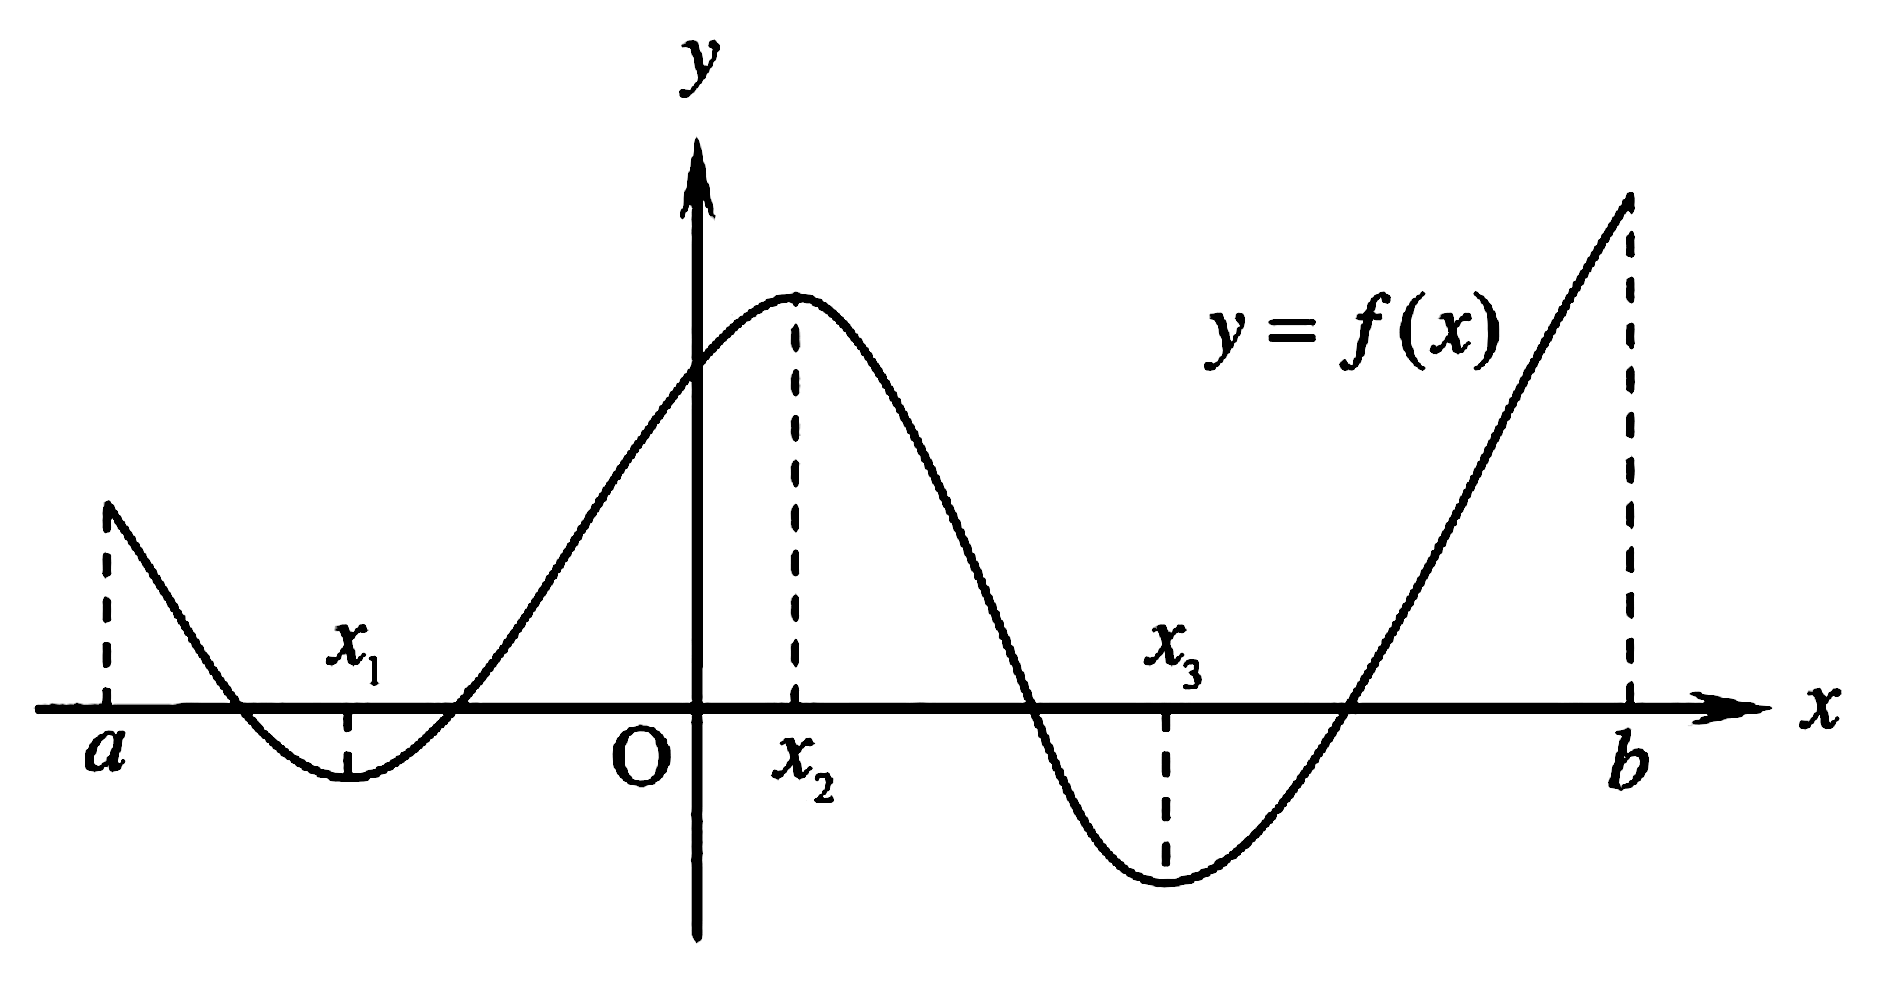
\includegraphics[scale=0.25]{assets/26-8.png}
\end{center}

\begin{center}
    \framebox{
        \parbox[t][1.6cm]{14cm}{ \addvspace{0.4cm} \centering \parbox{13.5cm}{If the function $f(x)$ is continuous in the close interval $[a,
                            b]$, then the function $f(x)$ must have the absolute maximum value and the
                absolute minimum value in the interval $[a, b]$.} }}
\end{center}

The function $f(x)$ that is continuous in the open interval $(a, b)$ may not
have the absolute maximum value and the absolute minimum value. For example,
the function $y = \dfrac{1}{x}$ is continuous in the interval $(0, \infty)$,
but it does not have the absolute maximum value and the absolute minimum value.
Also in the diagram above, if the domain is defined as the open interval $(a,
    b)$, then the function $f(x)$ only has the relative minimum value but not the
absolute minimum value.

From the diagram above, if the function is continuous in the interval $[a, b]$,
we just have to make comparison between all the extreme points and vertices of
the function to find the absolute maximum value and the absolute minimum value
of the function.

\subsection{Practice 4}

\noindent \hspace{1.2em}\textit{Find the absolute maximum value and the absolute minimum value of the following functions (Question 1 to 2):}
\begin{enumerate}
    \item $f(x) = 3x^3 - 9x + 5$, $[-2, 2]$
    \item $f(x) = x^4 - 2x^2 + 5$, $[-2, 3]$
    \item If $x + y = 8$, find the absolute minimum value of $x^2 + y^2$.
    \item A metal wire with a length of $100$cm is bent into a rectangle. Find the width
          and the length of the rectangle so that the area of the rectangle is the
          largest.
\end{enumerate}
\subsection{Exercise 26.4}

\noindent \hspace{1.2em}\textit{Find the absolute maximum value and the absolute minimum value of the following functions (Question 1 to 3):}
\begin{enumerate}
    \item $f(x)=5-36 x+3 x^2+4 x^3$, $[-1,2]$
    \item $f(x)=4 x^2\left(x^2-2\right)$, $[-1,3]$
    \item $f(x)=x^5-5 x^4+5 x^3$, $[0,4]$
    \item A metal wire with a length of $60$cm is bent into a rectangle. Find the width
          and the length of the rectangle so that the area of the rectangle is the
          largest.
    \item A metal wire with a length of $100$cm is cut into two sections. Each section is
          bent into a square. Find the length of these two sections of the wire so that
          the sum of the areas of the two squares is the smallest.
    \item As shown in the diagram below, a trapezium has three sides of length $10$cm.If
          the area of the trapezium is the largest, find the length of the fourth side.
          Hence, find the maximum area of the trapezium.
          \begin{center}
              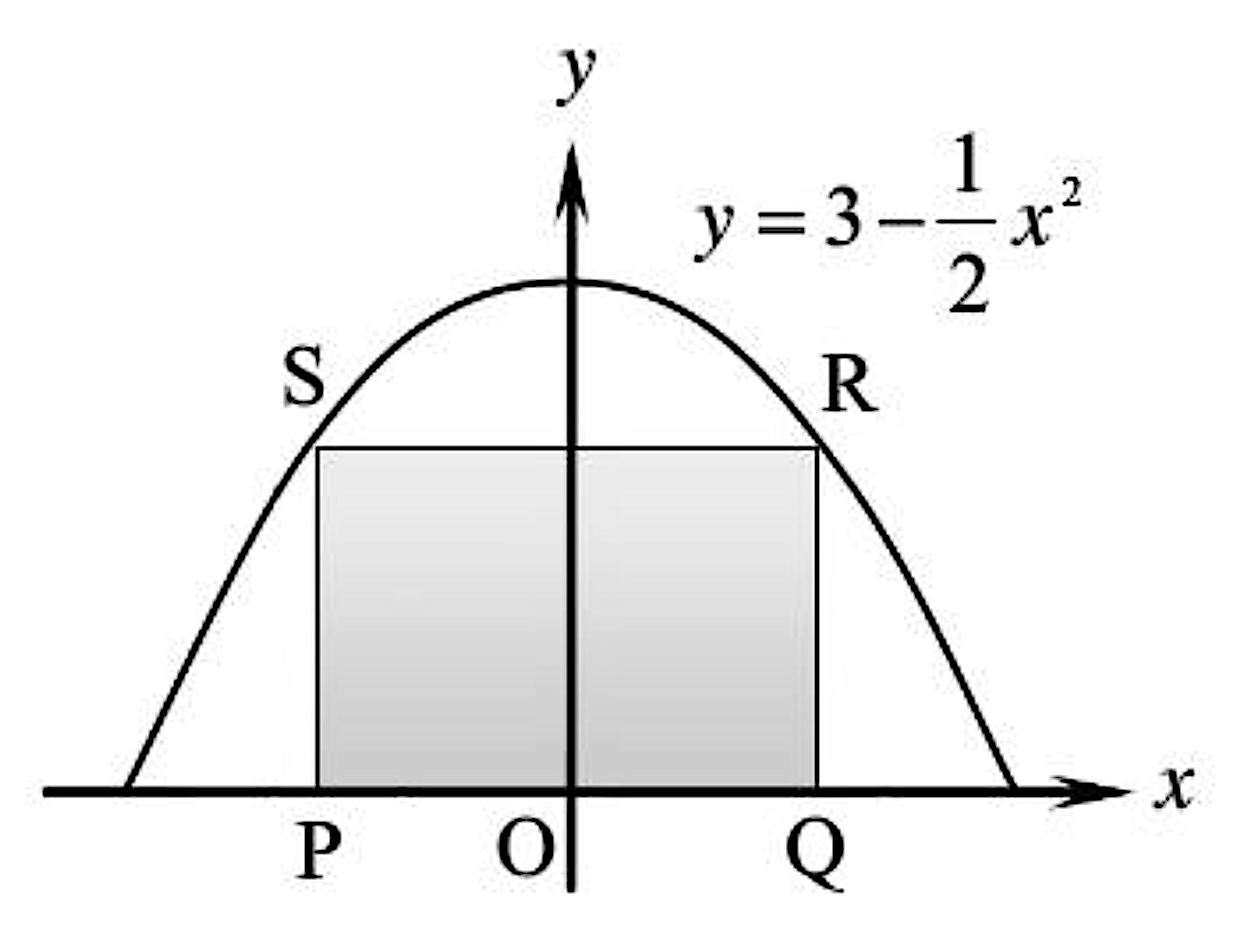
\includegraphics[scale=0.25]{assets/26-9.png}
          \end{center}
    \item A right cone has a slant height of $9$cm. Find the height of the cylinder such
          that the volume of the cylinder is the largest.
    \item A cylinder shaped can with lid has a volume of $250\pi$cm$^3$. Find the bottom
          radius and the height of the can so that the material used is the least.
    \item Split the number 20 into two parts such that one part is 4 times the reciprocal
          of another part, and the the sum of it with with 9 times the reciprocal of
          another part is the smallest.
    \item A metal wire with a length of $150$cm is split into two sections, and they are
          bent into a square and a circle respectively. Find the length of these two
          sections such that the sum of the area of the square and the circle is the
          smallest.
    \item As shown in the diagram below, a window is formed by a rectangle and a
          semicircle. The perimeter of the entire window is 300cm. If the area of the
          window is the largest, find the length of the rectangle. Hence, find the
          maximum area of the window.
          \begin{center}
              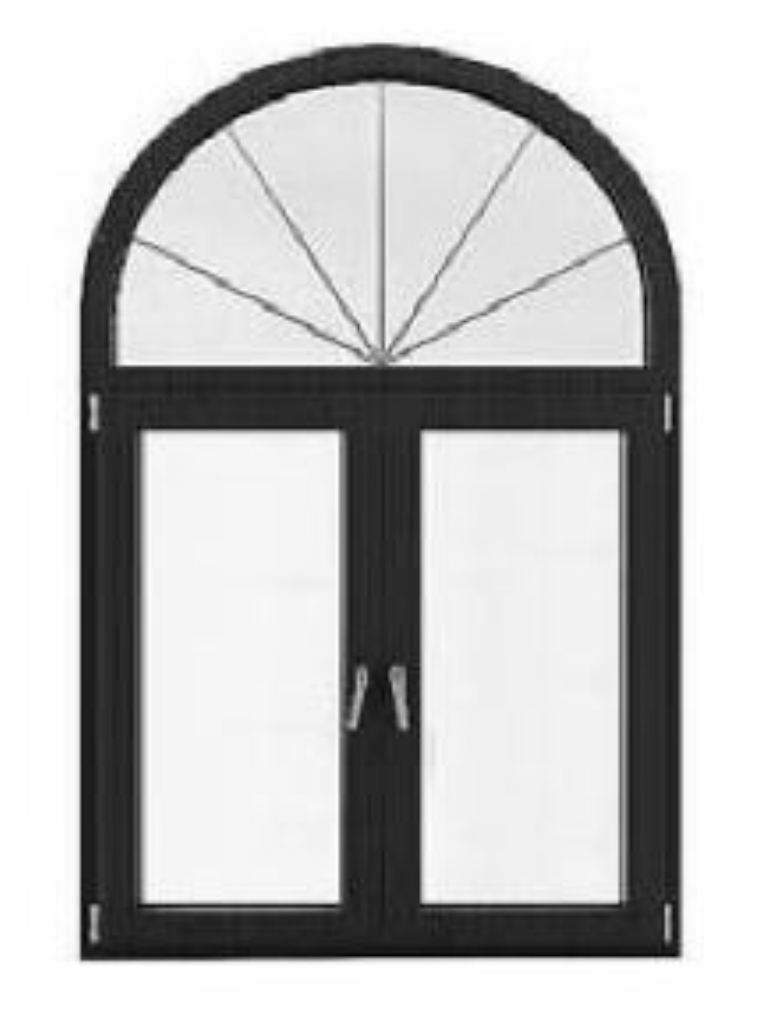
\includegraphics[scale=0.25]{assets/26-10.png}
          \end{center}
    \item In the diagram below, $PQRS$ is a rectangle, the coordinates of $P$ and $Q$ are
          $(-k, 0)$ and $(k, 0)$ respectively, where $k > 0$, and the two points $R$ and
          $S$ are on the curve $y = 3- \dfrac{1}{2}x^2$. Find the value of $k$ such that
          the area of the rectangle is the largest.
          \begin{center}
              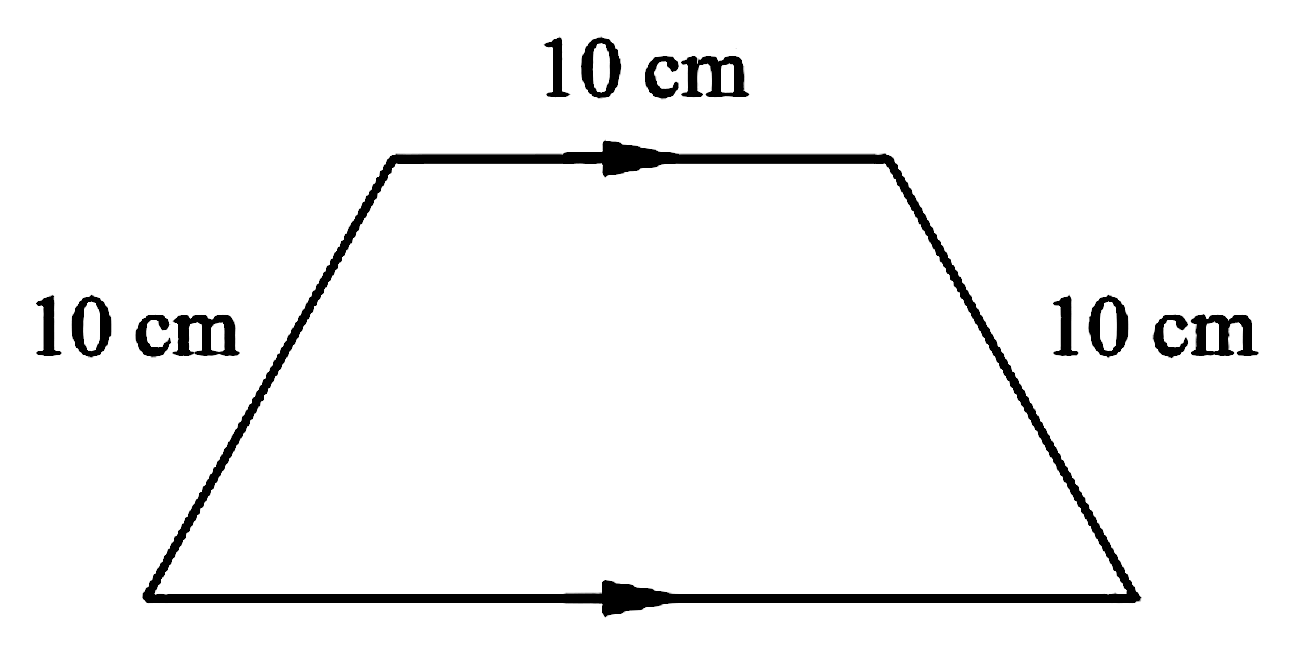
\includegraphics[scale=0.25]{assets/26-11.png}
          \end{center}
\end{enumerate}

\section{The Convexity and the Point of Inflection of Functions}

For a curve $y = f(x)$
\begin{enumerate}
    \item In a given interval, if the tangent line of the curve is always above the
          curve, then the curve convex up in the interval, as shown in the diagram below.
          \begin{center}
              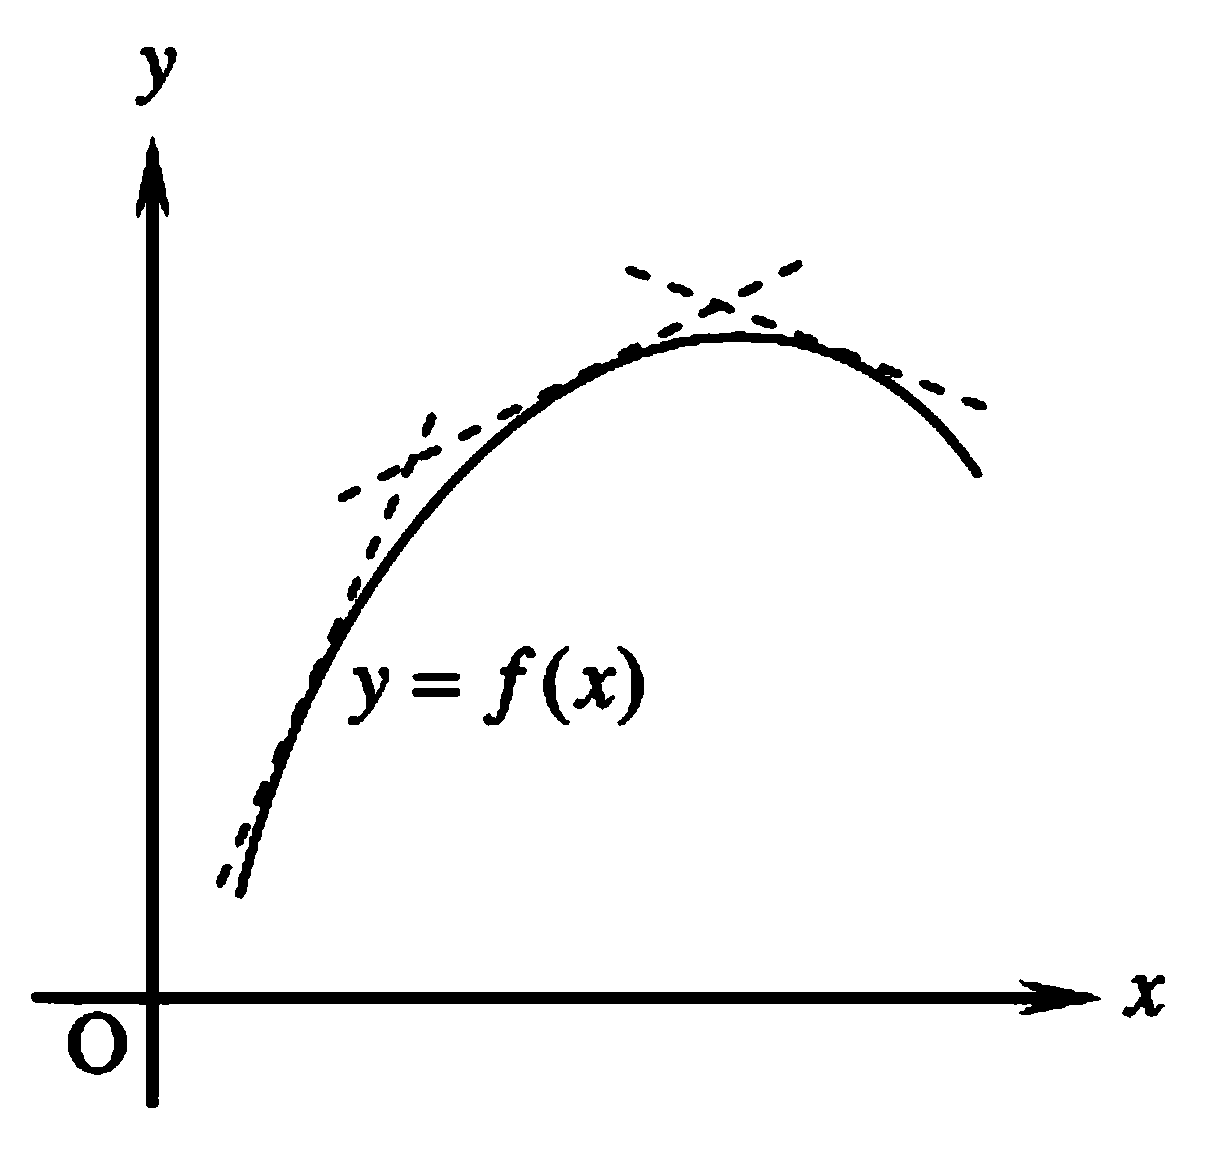
\includegraphics[scale=0.25]{assets/26-12.png}
          \end{center}
    \item In a given interval, if the tangent line of the curve is always below the
          curve, then the curve is convex down in the interval, as shown in the diagram
          below.
          \begin{center}
              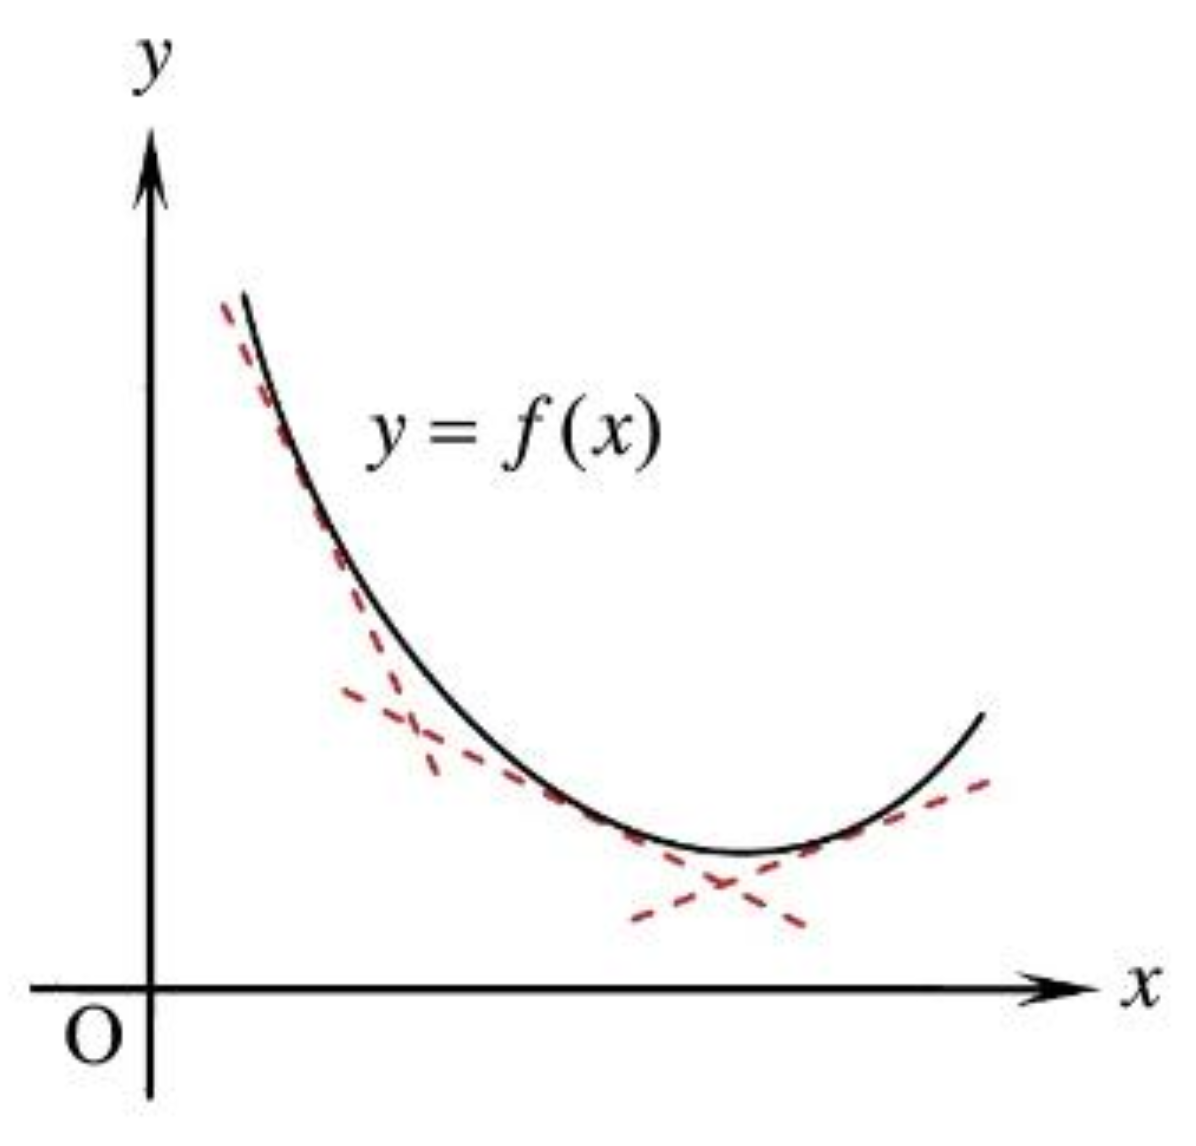
\includegraphics[scale=0.25]{assets/26-13.png}
          \end{center}
\end{enumerate}

If two sides of a point on a curve of a function $y = f(x)$ changes their
concavity, then the demarcation point is called the point of inflection of the
curve.

Now we discuss the way to determine the convexity and the point of inflection
of a function. In the diagram below, the left side of the point $x = x_0$
convex down, and the right side convex up.
\begin{center}
    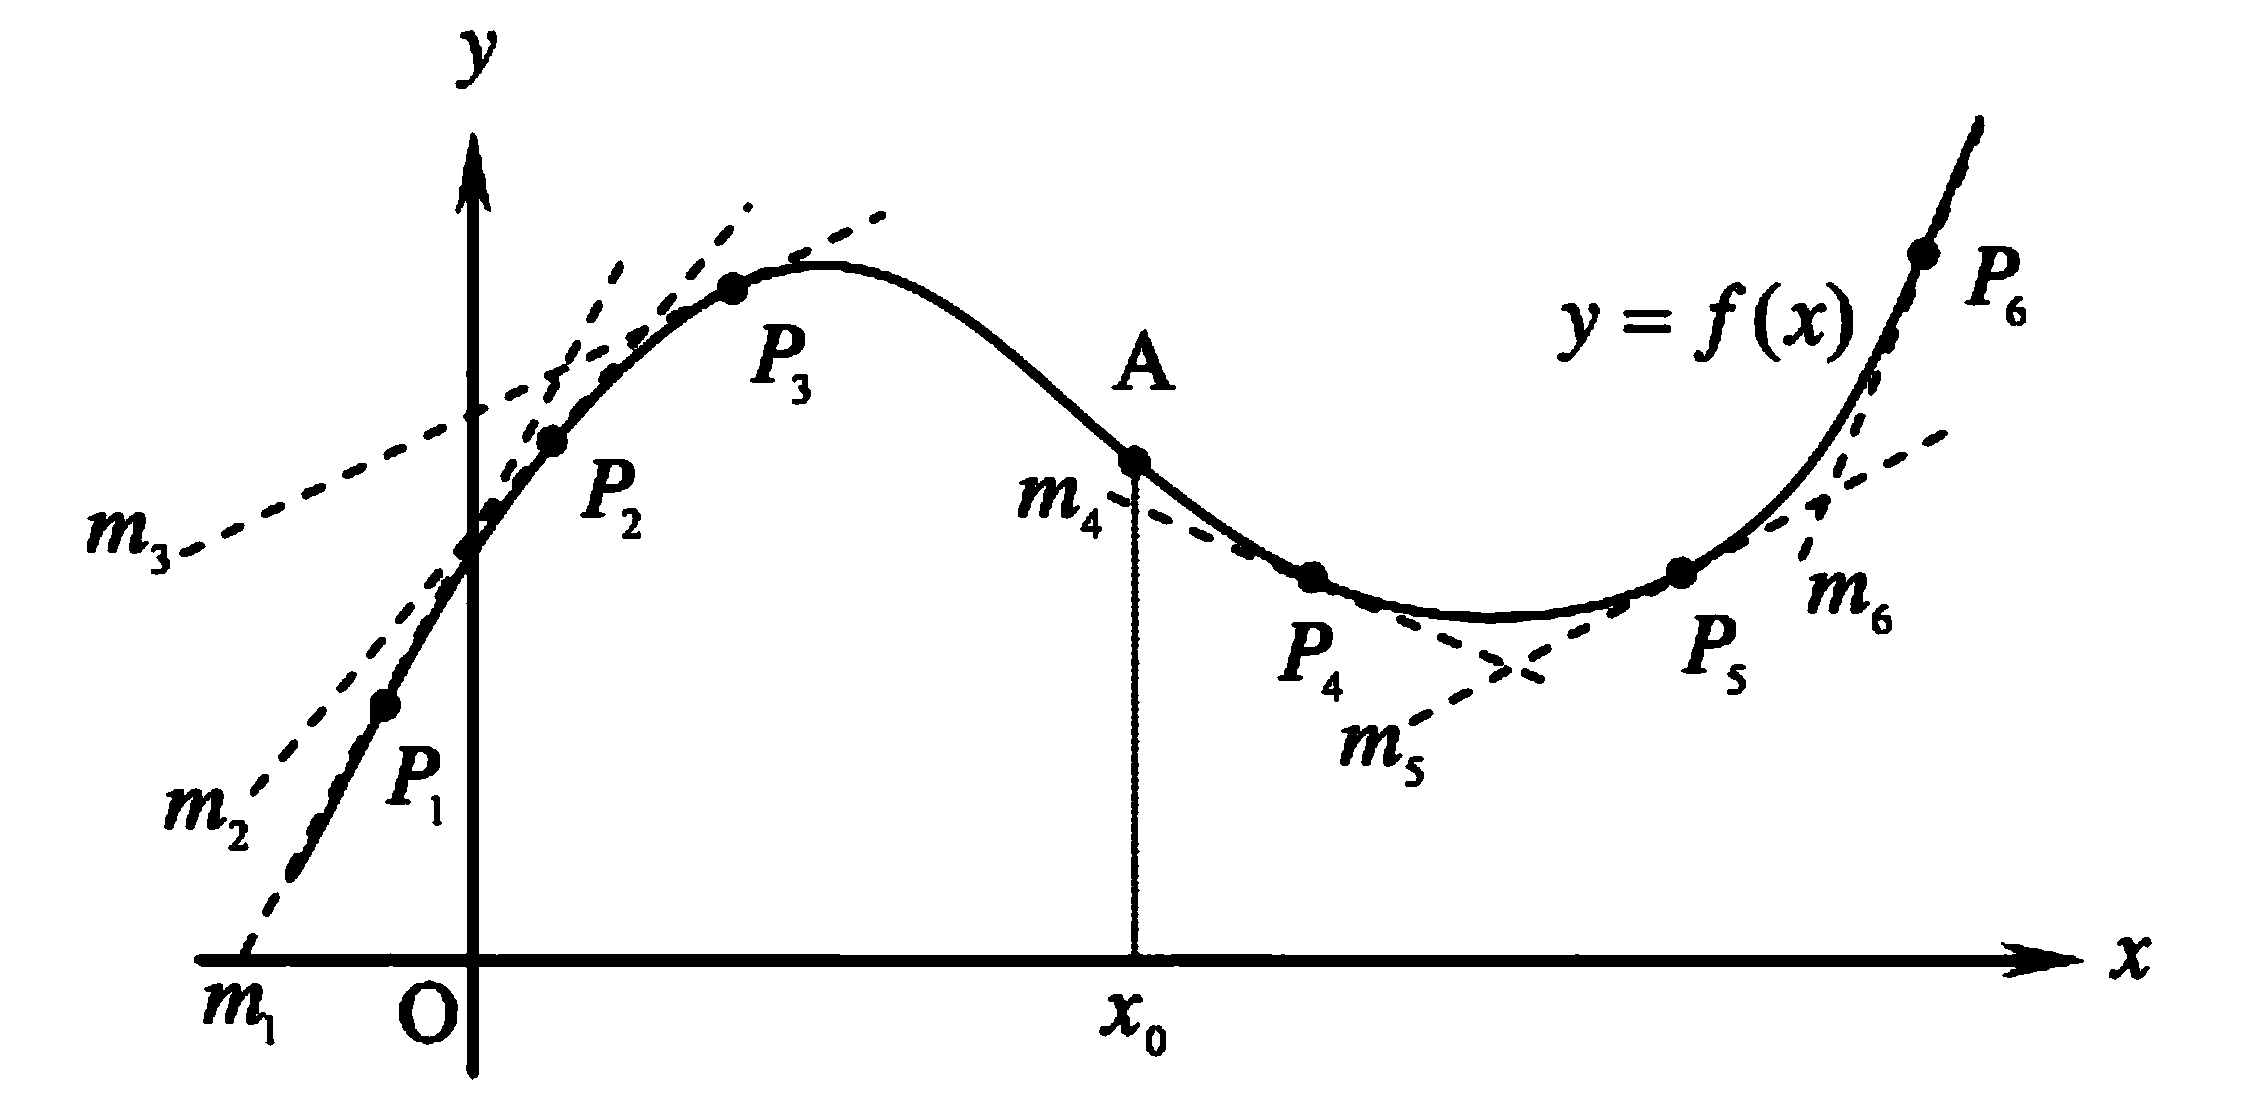
\includegraphics[scale=0.25]{assets/26-14.png}
\end{center}
In the interval $(-\infty, x_0)$ that convex up, when the tangents to the curve cut the curve at $P_1$, $P_2$, and $P_3$ respectively from left to right, the gradients of the tangent lines $m_1$, $m_2$, and $m_3$ are decreasing, i.e. the gradient of the tangent $f'(x)$ is decreasing.

In the interval $(x_0, \infty)$ that convex down, when the tangents to the
curve cut the curve at $P_4$, $P_5$, and $P_6$ respectively from left to right,
the gradients of the tangent lines $m_4$, $m_5$, and $m_6$ are increasing, i.e.
the gradient of the tangent $f'(x)$ is increasing.

We have the following theorem:
\begin{center}
    \framebox{
        \parbox[t][2.7cm]{14cm}{ \addvspace{0.4cm} \hspace{0.4cm}Let function $f(x)$ has
            second derivative $f''(x)$.
            \begin{itemize}[leftmargin=0.8cm]
                \item \parbox[t]{12.5cm}{If $f''(x) > 0$ in a given interval, then the curve is convex
                          up;}
                \item \parbox[t]{12.5cm}{If $f''(x) < 0$ in a given interval, then the curve is convex
                          down.}
            \end{itemize} }}
\end{center}

\subsection{Practice 5}
Find the following indefinite integral:
\begin{enumerate}
    \begin{multicols}{2}
        \item $\displaystyle\int\sin2x\cos2x dx$
        \sol{}
        \begin{flalign*}
            I & = \dfrac{1}{2}\int\sin4x dx & \\
              & = -\dfrac{1}{8}\cos4x + C
        \end{flalign*}
        \vfill{}\null{}

        \item $\displaystyle\int\cos^2 2x dx$
        \sol{}
        \begin{flalign*}
            I & = \int\dfrac{1 + \cos 4x}{2} dx                    & \\
              & = \dfrac{1}{2}\int dx + \dfrac{1}{2}\int\cos 4x dx & \\
              & = \dfrac{1}{2}x + \dfrac{1}{8}\sin 4x + C
        \end{flalign*}
    \end{multicols}
    \begin{multicols}{2}
        \item $\displaystyle\int\sin^3 x dx$
        \sol{}
        \begin{flalign*}
            I & = \int\sin^2 x\sin x dx                 & \\
              & = \int(1 - \cos^2 x)\sin x dx           & \\
              & = \int\sin x dx - \int\cos^2 x\sin x dx
        \end{flalign*}
        Let $u = \cos x$, $du = -\sin xdx$.
        \begin{flalign*}
            I & = -\int \cos x dx + \int u^2 du    & \\
              & = -\sin x + \dfrac{1}{3}u^3 + C    & \\
              & = \dfrac{1}{3}\cos^3 x -\sin x + C
        \end{flalign*}

        \item $\displaystyle\int\cos^3 x dx$
        \sol{}
        \begin{flalign*}
            I & = \int\cos^2 x\cos x dx                 & \\
              & = \int(1 - \sin^2 x)\cos x dx           & \\
              & = \int\cos x dx - \int\sin^2 x\cos x dx
        \end{flalign*}
        Let $u = \sin x$, $du = \cos xdx$.
        \begin{flalign*}
            I & = \int \cos x dx - \int u^2 du      & \\
              & = \sin x - \dfrac{1}{3}u^3 + C      & \\
              & = \sin x - \dfrac{1}{3}\sin^3 x + C
        \end{flalign*}
    \end{multicols}
    \begin{multicols}{2}
        \item $\displaystyle\int\tan^4 x\sec^2 x dx$
        \sol{}

        Let $u = \tan x$, $du = \sec^2 xdx$.
        \begin{flalign*}
            I & = \int u^4 du              & \\
              & = \dfrac{u^5}{5} + C       & \\
              & = \dfrac{1}{5}\tan^5 x + C
        \end{flalign*}
        \vfill{}\null{}
        \columnbreak
        \item $\displaystyle\int\tan^4\dfrac{x}{2} dx$
        \sol{}
        \begin{flalign*}
            I & = \int\tan^2\dfrac{x}{2}\tan^2\dfrac{x}{2} dx                             & \\
              & = \int\left(\sec^2\dfrac{x}{2} - 1\right)\tan^2\dfrac{x}{2} dx            & \\
              & = \int\sec^2\dfrac{x}{2}\tan^2\dfrac{x}{2} dx - \int\tan^2\dfrac{x}{2} dx
        \end{flalign*}
        Let $u = \tan\dfrac{x}{2}$, $du = \dfrac{1}{2}\sec^2\dfrac{x}{2}dx$.
        \begin{flalign*}
            I & = 2\int u^2 du - \int \tan^2\dfrac{x}{2} dx                     & \\
              & = \dfrac{2u^3}{3} - \int \left(\sec^2\dfrac{x}{2} - 1\right) dx & \\
              & = \dfrac{2u^3}{3} - \int \sec^2\dfrac{x}{2} dx + \int dx        & \\
              & = \dfrac{2}{3}\tan^3\dfrac{x}{2} - 2\tan\dfrac{x}{2} + x + C
        \end{flalign*}
    \end{multicols}
\end{enumerate}
\subsection{Practice 26.5}
\noindent \hspace{1.2em}\textit{Find the coordinates of the points of inflection of the following functions (Question 1 to 3):}
\begin{enumerate}
    \item $f(x)=x^3-6 x+4$
    \item $f(x)=x^3(4-x)$
    \item $f(x)=x^{\frac{7}{3}}$
\end{enumerate}

\noindent \hspace{1.2em}\parbox{\textwidth-1.2em}{\textit{Find the intervals where the following functions
        are convex up or convex down, and find the points of inflection of the
        functions (Question 4 to 6):}}
\begin{enumerate}[resume]
    \item $f(x)=-(x-2)^3$
    \item $f(x)=2 x^3-3 x^2-36 x+25$
    \item $f(x)=x^4-2 x^3+1$
\end{enumerate}

\noindent \hspace{1.2em}\parbox{\textwidth-1.2em}{\textit{Find the extreme values, the coordinates of the
        points of inflection, and the intervals where the following functions are
        convex up or convex down (Question 7 to 8):}}
\begin{enumerate}[resume]
    \item $f(x)=x(6-2 x)^2$
    \item $f(x)=-\dfrac{2}{1+x^2}$
\end{enumerate}

\section{Curve Sketching}

Having learnt the derivatives, we can use the concepts of the increasing and
decreasing of a function, the convexity and the point of inflection of a
function to sketch the curve of a function in a rather accurate way. Listed
below are the steps to sketch the curve of a function:
\begin{enumerate}
    \item Find the point of intersections of the curve with the axes;
    \item Solve the equation $f'(x) = 0$, and determine the intervals where the function
          is increasing or decreasing and the extreme values;
    \item Solve the equation $f''(x) = 0$, and determine the intervals where the curve is
          convex up or convex down and the points of inflection;
    \item Draw the curve according to the above information.
\end{enumerate}
The steps above are not necessarily to be followed in the order listed, and can be adjusted according to the actual situation.

\subsection{Practice 6}

Sketch the graph of the function $f(x) = x^3 - 3x^2 + 2$.
\subsection{Exercise 26.6}

Sketch the graph of the following functions (Question 1 to 3):

\begin{enumerate}
      \item $f(x)=\dfrac{1}{3} x^3-\dfrac{1}{2} x^2-2 x$
            \sol{}
            \vspace{-1cm}
            \begin{multicols}{2}
                  \begin{flalign*}
                        f(0)                                   & = 0                                                                     & \\
                        \dfrac{1}{3}x^3 - \dfrac{1}{2}x^2 - 2x & = 0                                                                     & \\
                        2x^3 - 3x^2 - 12x                      & = 0                                                                     & \\
                        x(2x^2 - 3x - 12)                      & = 0                                                                     & \\
                        x                                      & = 0 \text{ or } 2x^2 - 3x - 12 = 0                                      & \\
                                                               & = 0 \text{ or } x = \dfrac{3 \pm \sqrt{105}}{4}                           \\
                        f'(x)                                  & = x^2 - x - 2                                                           & \\
                        f''(x)                                 & = 2x - 1                                                                & \\
                        x^2 - x - 2                            & = 0                                                                     & \\
                        (x - 2)(x + 1)                         & = 0                                                                     & \\
                        x                                      & = 2 \text{ or } x = -1                                                  & \\
                        f(2)                                   & = \dfrac{1}{3}\left(2\right)^3 - \dfrac{1}{2}\left(2\right)^2 - 2(2)      \\
                                                               & = \dfrac{8}{3} - 2 - 4                                                    \\
                                                               & = -\dfrac{10}{3}                                                          \\
                        f(-1)                                  & = \dfrac{1}{3}\left(-1\right)^3 - \dfrac{1}{2}\left(-1\right)^2 - 2(-1)   \\
                                                               & = -\dfrac{1}{3} - \dfrac{1}{2} + 2                                        \\
                                                               & = \dfrac{7}{6}                                                            \\
                        f''(2)                                 & = 3 > 0                                                                   \\
                        f''(-1)                                & = -3 < 0
                  \end{flalign*}

                  \begin{flalign*}
                        2x - 1                     & = 0                                                                                                              & \\
                        x                          & = \dfrac{1}{2}                                                                                                   & \\
                        f\left(\dfrac{1}{2}\right) & = \dfrac{1}{3}\left(\dfrac{1}{2}\right)^3 - \dfrac{1}{2}\left(\dfrac{1}{2}\right)^2 - 2\left(\dfrac{1}{2}\right)   \\
                                                   & = \dfrac{1}{24} - \dfrac{1}{8} - 1                                                                                 \\
                                                   & = -\dfrac{13}{12}
                  \end{flalign*}
                  $x$-intercepts: $\left(0, 0\right)$, $\left(\dfrac{3 - \sqrt{105}}{4}, 0\right)$, $\left(\dfrac{3 + \sqrt{105}}{4}, 0\right)$

                  \noindent $y$-intercept: $(0, 0)$

                  \noindent Relative maximum: $\left(-1, \dfrac{7}{6}\right)$

                  \noindent Relative minimum: $\left(2, -\dfrac{10}{3}\right)$

                  \noindent Points of inflection: $\left(\dfrac{1}{2}, -\dfrac{13}{12}\right)$

                  \noindent Convex up: $\left(-\infty, \dfrac{1}{2}\right)$

                  \noindent Convex down: $\left(\dfrac{1}{2}, \infty\right)$
            \end{multicols}
            \vfill\null
            \begin{center}
                  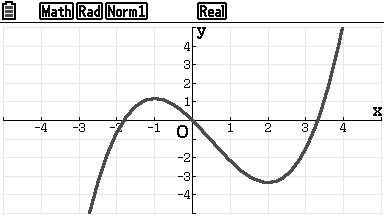
\includegraphics[scale=0.7]{26-graph2.png}
            \end{center}
            \vfill\null
            \newpage

      \item $f(x)=x^4-32 x+10$
            \sol{}
            \vspace{-0.6cm}
            \begin{vwcol}[widths={0.3,0.7},justify=flush,rule=0pt,indent=1em]
                  \begin{flalign*}
                        f(0)      & = 10               & \\
                        f'(x)     & = 4x^3 - 32        & \\
                        f''(x)    & = 12x^2            & \\
                        4x^3 - 32 & = 0                & \\
                        x         & = 2                & \\
                        f(2)      & = 2^4 - 32(2) + 10   \\
                                  & = -38              & \\
                        f''(2)    & = 48 > 0           & \\
                        12x^2     & = 0                & \\
                        x         & = 0                & \\
                        f(0)      & = 10
                  \end{flalign*}
                  y-intercept: $(0, 10)$

                  \noindent Relative minimum: $(2, -38)$

                  \noindent Points of inflection: $(0, 10)$

                  \noindent Convex down: $(-\infty, \infty)$
                  \newpage
                  \vspace*{2cm}
                  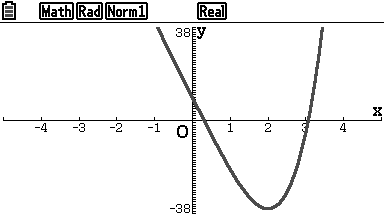
\includegraphics[scale=0.7]{26-graph3.png}
            \end{vwcol}

      \item $f(x)=(x-1)^3(x-2)$
            \sol{}
            \vspace{-1cm}
            \begin{multicols}{2}
                  \begin{flalign*}
                        f(0)                         & = 2                                                     & \\
                        (x-1)^3(x-2)                 & = 0                                                       \\
                        x                            & = 1 \text{ or } x = 2                                     \\
                        f'(x)                        & = 3(x-1)^2(x-2) + (x-1)^3                                 \\
                                                     & = (x-1)^2(3x-6+x-1)                                       \\
                                                     & = (x-1)^2(4x-7)                                           \\
                        f''(x)                       & = 2(x-1)(4x-7) + (x-1)^2(4)                               \\
                                                     & = 2(x-1)(4x-7+2x-2)                                       \\
                                                     & = 2(x-1)(6x-9)                                            \\
                                                     & = 6(x-1)(2x-3)                                            \\
                        (x-1)^2(4x-7)                & = 0                                                       \\
                        x                            & = 1 \text{ or } x = \dfrac{7}{4}                          \\
                        f(1)                         & = 0                                                       \\
                        f\left(\dfrac{7}{4}\right)   & = \left(\dfrac{3}{4}\right)^3\left(-\dfrac{1}{4}\right)   \\
                                                     & = -\dfrac{27}{256}                                        \\
                        f''(1)                       & = 0                                                       \\
                        f''\left(\dfrac{7}{4}\right) & = 6\left(\dfrac{3}{4}\right)\left(\dfrac{7}{2}-3\right)   \\
                                                     & = \dfrac{9}{4} > 0                                      &
                  \end{flalign*}

                  \begin{flalign*}
                        6(x-1)(2x-3)               & = 0                                                     \\
                        x                          & = 1 \text{ or } x = \dfrac{3}{2}                        \\
                        f(1)                       & = 0                                                     \\
                        f\left(\dfrac{3}{2}\right) & = \left(\dfrac{1}{2}\right)^3\left(-\dfrac{1}{2}\right) \\
                                                   & = -\dfrac{1}{16}
                  \end{flalign*}
                  $x$-intercepts: $(1, 0)$, $\left(2, 0\right)$

                  \noindent $y$-intercept: $(0, 2)$

                  \noindent Relative minimum: $\left(\dfrac{7}{4}, -\dfrac{27}{256}\right)$

                  \noindent Points of inflection: $\left(1, 0\right)$, $\left(\dfrac{3}{2}, -\dfrac{1}{16}\right)$

                  \noindent Convex downwards: $\left(-\infty, 1\right)$, $\left(\dfrac{3}{2}, \infty\right)$

                  \noindent Convex upwards: $\left(1, \dfrac{3}{2}\right)$
            \end{multicols}
            \begin{center}
                  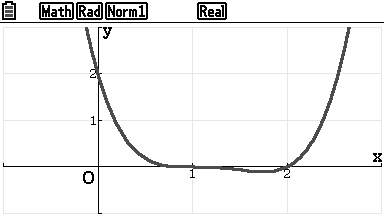
\includegraphics[scale=0.6]{26-graph4.png}
            \end{center}

      \item Given the function $f(x) = x^3(4-x)$.
            \begin{enumerate}
                  \begin{multicols}{2}
                        \item Find the extreme values and the intervals of increasing and decreasing of
                        $f(x)$. \sol{}
                        \begin{flalign*}
                              f(x)        & = 4x^3 - x^4      \\
                              f'(x)       & = 12x^2 - 4x^3    \\
                                          & = 4x^2(3 - x)     \\
                              4x^2(3 - x) & = 0               \\
                              x = 0       & \text{ or } x = 3 \\
                              f(0)        & = 0               \\
                              f(3)        & = 27              \\
                              f''(x)      & = 24x - 12x^2     \\
                              f''(0)      & = 0               \\
                              f''(3)      & = 36 > 0
                        \end{flalign*}
                        $\therefore$ Relative maximum: $f(3) = 27$

                        In the interval $(-\infty, 0)$, $f'(x) > 0$, so $f(x)$ is increasing in the
                        interval $(-\infty, 0]$.

                        In the interval $(0, 3)$, $f'(x) > 0$, so $f(x)$ is increasing in the interval
                        $[0, 3]$.

                        In the interval $(3, \infty)$, $f(x)$ is decreasing in the interval $[3,
                                          \infty)$. \columnbreak

                                                \item Find the points of inflection and the intervals of convexity and concavity of
                                          $f(x)$. \sol{}
                                                \begin{flalign*}
                                                      24x - 12x^2 & = 0               \\
                                                      x(2 - x)    & = 0               \\
                                                      x = 0       & \text{ or } x = 2 \\
                                                      f(0)        & = 0               \\
                                                      f(2)        & = 16
                                                \end{flalign*}
                                          $\therefore$ Point of inflection: $(2, 16)$, $(0, 0)$

                                                In the interval $(-\infty, 0)$, $f''(x) < 0$, so $f(x)$ is convex upward in the
                                                interval $(-\infty, 0]$.

                        In the interval $(0, 2)$, $f''(x) < 0$, so $f(x)$ is convex upward in the
                        interval $[0, 2]$.

                        In the interval $(2, \infty)$, $f''(x) > 0$, so $f(x)$ is convex downward in
                        the interval $[2, \infty)$.
                  \end{multicols}

                  \item Hence, sketch the graph of $f(x)$. \sol{}
                        \begin{center}
                              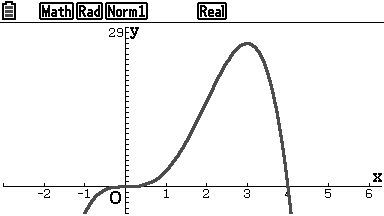
\includegraphics[scale=0.6]{26-graph5.png}
                        \end{center}
            \end{enumerate}
\end{enumerate}

\section{Rate of Change and Related Rate of Change}

The derivative of the function $y = f(x)$ at the point $x = x_0$ is known as
the rate of change of the dependent value $y$ with respect to the independent
value $x$ at the point $x = x_0$. For example, $\dfrac{d y}{d x} = 3$ means
that when $x$ increases by $1$ unit, $y$ increases by $3$ units, i.e. $y$ and
$x$ are both changing, and they are changing in the ratio of $3:1$.

The same can be said that the derivative of the area function $A = A(t)$ at the
time $t = t_0$ is the rate of change of the area with respect to the time at
the time $t = t_0$. When the rate of change of the area at $t = t_0$ is
$\dfrac{d A}{d t} = 4$cm$^2$/s, it means that the area is increasing in the
rate of 4 square centimetres per second; while $\dfrac{d A}{d t} = -4$cm$^2$/s
means that the area is decreasing in the rate of 4 square centimetres per
second.

If multiple variables are correlated by a specific relationship, these
variables are all changing with respect to time, then there must be some kind
of bonds between their respective rate of changes. This relationship between
the rate of changes is called the related rate of change. If $y = f(x)$ is the
function of $x$, and $x$ changes with respect to $t$, then since $y$ is
changing with respect to $x$, $y$ is also changing with respect to $t$. In
other words, $y$ is also a function of the time $t$. HEnce, from the chain
rule, we can obtain the following relationship:
\begin{cequation}
    \dfrac{dy}{dt} = \dfrac{dy}{dx} \cdot \dfrac{dx}{dt}
\end{cequation}
i.e. the rate of change of $y$ is correlated to the rate of change of $x$.

\subsection{Practice 7}
\begin{enumerate}
      \begin{multicols}{2}
            \item A drop of ink gradually spread after being dropped onto a piece of paper. At
            $t$ seconds, its area is $A = \left(3t^2 + \dfrac{1}{5}t + 2\right)$mm$^2$.
            Find the rate of change of the ink spread at $t = 2$ second. \sol{}
            \begin{flalign*}
                  \dfrac{dA}{dt} & = 6t + \dfrac{1}{5}
            \end{flalign*}
            When $t = 2$,
            \begin{flalign*}
                  \dfrac{dA}{dt} & = 6(2) + \dfrac{1}{5}      \\
                                 & = 12 + \dfrac{1}{5}        \\
                                 & = \dfrac{61}{5}            \\
                                 & = 12.2\text{mm}^2\text{/s}
            \end{flalign*}
            \vfill\null

            \item The radius of a sphere increases at a rate of $3$cm/s. When the radius is
            $5$cm, find the rate of change of the surface area of the sphere. \sol{}
            \begin{flalign*}
                  \dfrac{dr}{dt} & = 3\text{cm/s}                      \\
                  A              & = 4\pi r^2                          \\
                  \dfrac{dA}{dr} & = 8\pi r                            \\
                  \dfrac{dA}{dt} & = \dfrac{dA}{dr}\cdot\dfrac{dr}{dt} \\
                                 & = 8\pi r\cdot 3\text{cm/s}          \\
                                 & = 24\pi r\text{cm}^2\text{/s}
            \end{flalign*}
            When $r = 5$,
            \begin{flalign*}
                  \dfrac{dA}{dt} & = 24\pi(5)\text{cm}^2\text{/s} \\
                                 & = 120\pi\text{cm}^2\text{/s}
            \end{flalign*}
      \end{multicols}
\end{enumerate}
\subsection{Exercise 26.7}
\begin{enumerate}
    \item Water is poured into a container, the relationship between the volume of the
          water and the time is $V = (2t^2 + 3t)$cm$^3$. WHen $t = 3$s, find the rate of
          change of the volume of the water.
    \item One throws a piece of stone into the water. The radius of the ripple on the
          water surface caused by the stone is increasing at a rate of $0.1$m/s. When the
          radius is $1$m, find the rate of change of the area of the ripple.
    \item The side length of a square is increasing at a rate of $3$cm per second. When
          the side length is $15$cm, find the rate of change of its area.
    \item A cube expanded after being heated, the rate of change of its side length is
          $5$cm/s. When the side length is $4$cm, find the rate of change of its area.
    \item The radius of a sphere increases by 1cm per second. When the radius is 3cm,
          find the rate of change of its volume.
    \item The area of a circle increases by 5cm$^2$ per minute. When the circumference of
          the circle is 40cm find the rate of change of its radius.
    \item The volume of a sphere decreases at a rate of $12\pi$cm$^3$ per minute. When
          the radius of the sphere is 6cm, find the rate of change of its radius and
          surface area.
    \item The surface area of a sphere increase at a rate of $10$cm$^2$/s. When its
          radius is 5cm, find the rate of change of its radius and volume.
    \item Water is poured into the cone shaped container as shown in the diagram below,
          the rate of rising of the water surface is $1$cm per second. When the depth of
          the water is $2m$, find the rate of change of the water volume.
          \begin{center}
              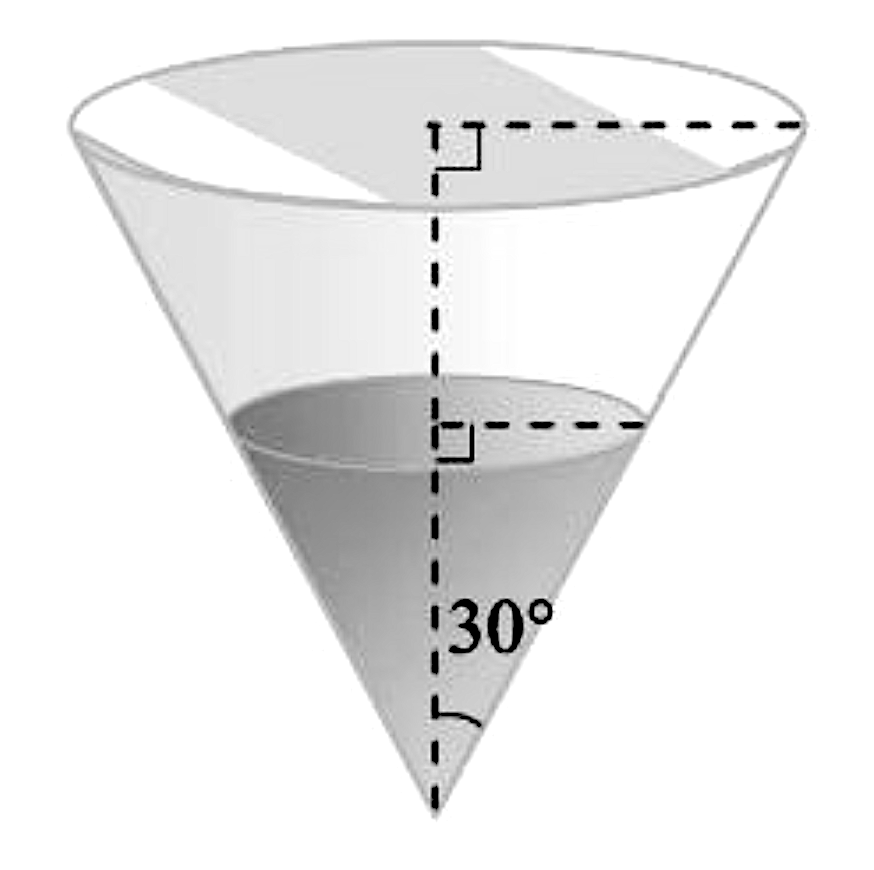
\includegraphics[scale=0.25]{assets/26-15.png}
          \end{center}
    \item The radius $r$ of a solid cylinder decreases by $0.04$cm per second, its height
          constantly equal to 20cm. When the radius is 2cm, find the rate of change of
          the surface area of the cylinder.
    \item Given the function $y = x^3 + 10$. When the rate of change of $y$ is 27 times
          the rate of change of $x$, find the value of $x$.
    \item Water is poured ito a cone shaped container facing downwards with a height of
          18m and a base radius of 24m. WHen the height of the water is 6m, find the rate
          of rising of the water surface.
\end{enumerate}


\section{Approximate Calculation}

In the previous chapter, we have learnt that the derivative of the function $y
    = f(x)$ is
\begin{cequation}
    \dfrac{dy}{dx} = \lim_{\Delta x \to 0}\dfrac{\Delta y}{\Delta x} = \lim_{\Delta x \to 0}\dfrac{f(x + \Delta x) - f(x)}{\Delta x}
\end{cequation}
From the definition of limit, we know that when $\Delta x$ is small enough,
\begin{cequation}
    \dfrac{\Delta y}{\Delta x} = \dfrac{\Delta y}{\Delta x} \approx \dfrac{f(x + \Delta x) - f(x)}{\Delta x}
\end{cequation}
Hence,
\begin{center}
    \framebox{
        \parbox[t][1.2cm]{9cm}{ \addvspace{0.25cm} \centering $\Delta y \approx
                \dfrac{dy}{dx}\Delta x$ }}
\end{center}
or $f(x + \Delta x) - f(x) \approx f'(x)\Delta x$, i.e.
\begin{center}
    \framebox{
        \parbox[t][1.2cm]{9cm}{ \addvspace{0.45cm} \centering $f(x + \Delta x) \approx f(x)
                + f'(x)\Delta x$ }}
\end{center}

The expression above is a simple formula for approximate calculation that can
be used to find the approximate value of a function.
\begin{center}
    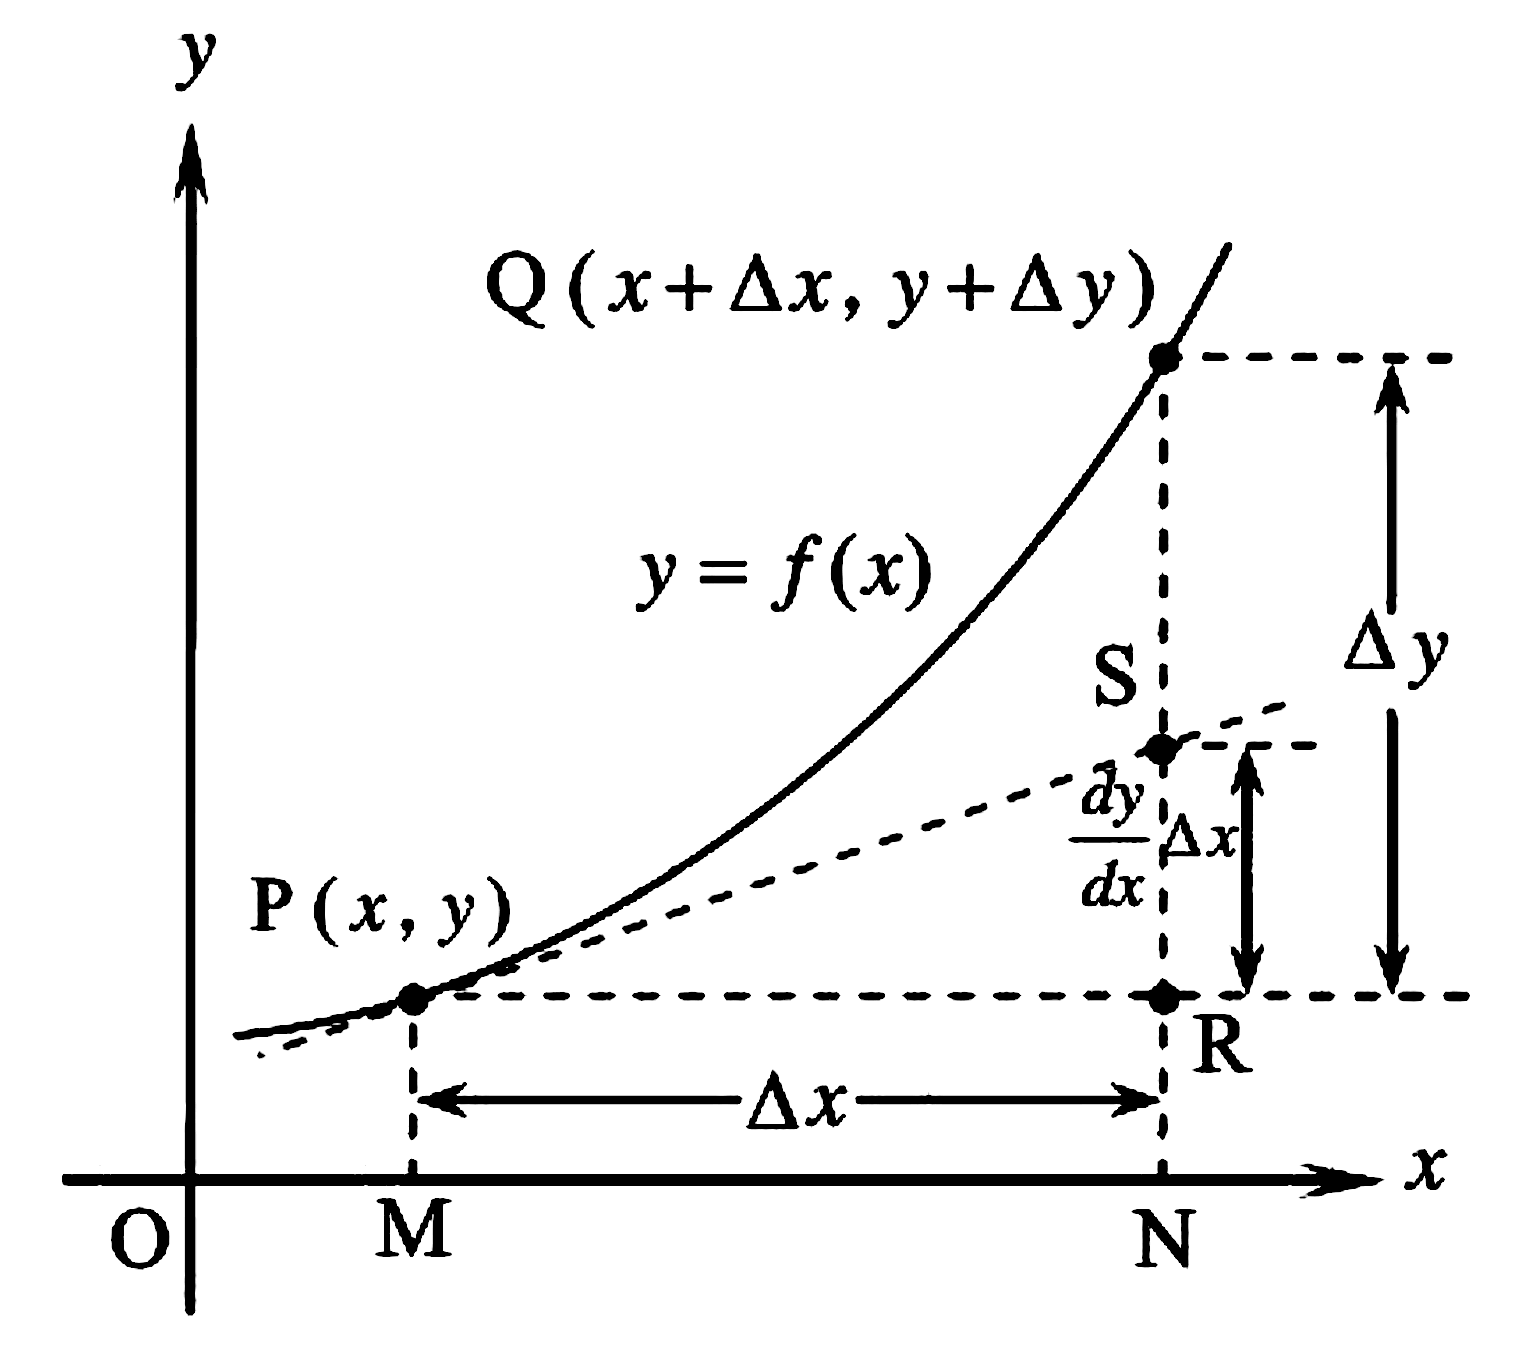
\includegraphics[scale=0.25]{assets/26-16.png}
\end{center}

\subsection{Practice 8}

\begin{enumerate}
      \item The side length of a cube increases from 1cm to $1.01$cm, how much does its
            surface area increase approximately? \sol{}

            Let the side length be $x$cm, then the surface area is $A = 6x^2$.
            \begin{flalign*}
                  \dfrac{dA}{dx}             & = 12x                  & \\
                  \dfrac{\Delta A}{\Delta x} & \approx \dfrac{dA}{dx} & \\
                  \Delta A                   & \approx 12x\Delta x
            \end{flalign*}
            \vspace{-0.8em}
            When $x = 1$cm, $\Delta x = 0.01$cm,
            \begin{flalign*}
                  \Delta A & \approx 12(1)(0.01) = 0.12\text{cm}^2 &
            \end{flalign*}
            $\therefore$ The surface area increases by $0.12$cm$^2$ approximately.

            \begin{multicols}{2}
                  \item After a metal ball was heated, its radius had increased form 4cm to $4.01$cm.
                  Find the approximate increment of its volume and surface area. \sol{}

                  Let the radius be $r$cm, then the volume is $V = \dfrac{4}{3}\pi r^3$ and the
                  surface area is $A = 4\pi r^2$.
                  \begin{flalign*}
                        \dfrac{dV}{dr}             & = 4\pi r^2               & \\
                        \dfrac{dA}{dr}             & = 8\pi r                 & \\
                        \dfrac{\Delta V}{\Delta r} & \approx \dfrac{dV}{dr}   & \\
                        \Delta V                   & \approx 4\pi r^2\Delta r & \\
                        \dfrac{\Delta A}{\Delta r} & \approx \dfrac{dA}{dr}   & \\
                        \Delta A                   & \approx 8\pi r\Delta r
                  \end{flalign*}
                  When $r = 4$cm, $\Delta r = 0.01$cm,
                  \begin{flalign*}
                        \Delta V & \approx 4\pi(4)^2(0.01) & \\
                                 & = 0.64\pi\text{cm}^3    & \\
                        \Delta A & \approx 8\pi(4)(0.01)   & \\
                                 & = 0.32\pi\text{cm}^2
                  \end{flalign*}
                  $\therefore$ The volume increases by $0.64\pi$cm$^3$ and the surface area increases by $0.32\pi$cm$^2$ approximately.
                  \columnbreak
                  \item Find the approximate value of $\sqrt{15}$. \sol{}
                  \begin{flalign*}
                        f(x)                       & = \sqrt{x}                           & \\
                        f'(x)                      & = \dfrac{1}{2\sqrt{x}}               & \\
                        \dfrac{\Delta f}{\Delta x} & \approx \dfrac{df}{dx}               & \\
                        \Delta f                   & \approx \dfrac{1}{2\sqrt{x}}\Delta x
                  \end{flalign*}
                  When $x = 16$, $\Delta x = -1$,
                  \begin{flalign*}
                        \Delta f & \approx \dfrac{1}{2\sqrt{16}}(-1) & \\
                                 & = -\dfrac{1}{8}                   & \\
                                 & = -0.125
                  \end{flalign*}
                  $\therefore$ $\sqrt{15} \approx \sqrt{16} - 0.125 = 3.875$.
            \end{multicols}
\end{enumerate}


\subsection{Exercise 26.8}
\begin{enumerate}
      \begin{multicols}{2}
            \item The side length of a square increased from 4cm to $4.001$cm, how much does its
            area increase approximately? \sol{}

            Let $x$ be the side length of the cube, then the area of the cube is $A = x^2$.
            \begin{flalign*}
                  \dfrac{dA}{dx}             & = 2x                            & \\
                  \dfrac{\Delta A}{\Delta x} & \approx \dfrac{dA}{dx} \Delta x & \\
                  \Delta A                   & \approx 2x \Delta x
            \end{flalign*}
            When $x = 4$, $\Delta x = 0.001$,
            \begin{flalign*}
                  \Delta A & \approx 2(4)(0.001) & \\
                           & = 0.008\text{cm}^2
            \end{flalign*}
            $\therefore$ The area of the square increases by $0.008\text{cm}^2$ approximately.

            \item The radius of a circle increases from 3cm to $3.01$cm, find the approximate
            increment of its area. \sol{}

            Let $r$ be the radius of the circle, then the area of the circle is $A = \pi
                  r^2$.
            \begin{flalign*}
                  \dfrac{dA}{dr}             & = 2\pi r                        & \\
                  \dfrac{\Delta A}{\Delta r} & \approx \dfrac{dA}{dr} \Delta r & \\
                  \Delta A                   & \approx 2\pi r \Delta r
            \end{flalign*}
            When $r = 3$, $\Delta r = 0.01$,
            \begin{flalign*}
                  \Delta A & \approx 2\pi(3)(0.01) & \\
                           & = 0.06\pi\text{cm}^2
            \end{flalign*}
            $\therefore$ The area of the circle increases by $0.06\pi\text{cm}^2$
            approximately.
      \end{multicols}

      \begin{multicols}{2}
            \item The radius of a sphere decrease from 3cm to $2.98$cm, find the approximate
            decrement of its volume. \sol{}

            Let $r$ be the radius of the sphere, then the volume of the sphere is $V =
                  \dfrac{4}{3}\pi r^3$.
            \begin{flalign*}
                  \dfrac{dV}{dr}             & = 4\pi r^2                      & \\
                  \dfrac{\Delta V}{\Delta r} & \approx \dfrac{dV}{dr} \Delta r & \\
                  \Delta V                   & \approx 4\pi r^2 \Delta r
            \end{flalign*}
            When $r = 3$, $\Delta r = -0.02$,
            \begin{flalign*}
                  \Delta V & \approx 4\pi(3)^2(-0.02) & \\
                           & = -0.72\pi\text{cm}^3
            \end{flalign*}
            $\therefore$ The volume of the sphere decreases by $0.72\pi\text{cm}^3$
            approximately.

            \item Let $y = 3x^5$. If $x$ is decreased by $0.2\%$, how many percent does $y$
            decrease approximately? \sol{}
            \begin{flalign*}
                  \dfrac{dy}{dx}             & = 15x^4                         & \\
                  \dfrac{\Delta y}{\Delta x} & \approx \dfrac{dy}{dx} \Delta x & \\
                  \Delta y                   & \approx 15x^4 \Delta x
            \end{flalign*}
            When $\Delta x = -0.002x$,
            \begin{flalign*}
                  \Delta y                         & \approx 15x^4(-0.002x)                & \\
                                                   & = -0.03x^5                            & \\
                  \dfrac{\Delta y}{y} \times 100\% & = \dfrac{-0.03x^5}{3x^5} \times 100\% & \\
                                                   & = -1\%
            \end{flalign*}
            $\therefore$ $y$ decreases by $1\%$ approximately.
      \end{multicols}

      \item If the side length of a cube increases by $1\%$, how many percent does its
            volume increase approximately? \sol{}

            Let $x$ be the side length of the cube, then the volume of the cube is $V =
                  x^3$.
            \begin{flalign*}
                  \dfrac{dV}{dx}             & = 3x^2                          & \\
                  \dfrac{\Delta V}{\Delta x} & \approx \dfrac{dV}{dx} \Delta x & \\
                  \Delta V                   & \approx 3x^2 \Delta x
            \end{flalign*}
            When $\Delta x = 0.01x$,
            \begin{flalign*}
                  \Delta V                         & \approx 3x^2(0.01x)                 & \\
                                                   & = 0.03x^3                           & \\
                  \dfrac{\Delta V}{V} \times 100\% & = \dfrac{0.03x^3}{x^3} \times 100\% & \\
                                                   & = 3\%
            \end{flalign*}
            $\therefore$ The volume of the cube increases by $3\%$ approximately.

      \item Let the surface area of a solid right cylinder with a height of 16cm and a
            radius of $r$cm be $A$.
            \begin{enumerate}
                  \item Prove that $\dfrac{dA}{dr} = 4\pi(r+8)$. \prooff{}
                        \begin{flalign*}
                              A              & = 2\pi r^2 + 2\pi rh    &      \\
                                             & = 2\pi r^2 + 2\pi r(16) &      \\
                                             & = 2\pi r^2 + 32\pi r    &      \\
                              \dfrac{dA}{dr} & = 4\pi r + 32\pi        &      \\
                                             & = 4\pi(r+8)             & \qed
                        \end{flalign*}

                  \item If the height of the right cylinder remains the same, using the result obtained
                        from (a), find, when the radius of the right cylinder increases from 4cm to
                        $4.02$cm, the approximate increment of its surface area. \sol{}
                        \begin{flalign*}
                              \dfrac{dA}{dr}             & = 4\pi(r+8)                     & \\
                              \dfrac{\Delta A}{\Delta r} & \approx \dfrac{dA}{dr} \Delta r & \\
                              \Delta A                   & \approx 4\pi(r+8) \Delta r
                        \end{flalign*}
                        When $r = 4$, $\Delta r = 0.02$,
                        \begin{flalign*}
                              \Delta A & \approx 4\pi(4+8)(0.02) & \\
                                       & = 0.96\pi\text{cm}^2
                        \end{flalign*}
                        $\therefore$ The surface area of the right cylinder increases by $0.96\pi\text{cm}^2$ approximately.
            \end{enumerate}
            \vfill\null

      \item If $y = \dfrac{1}{\sqrt{x}}$, find $\dfrac{dy}{dx}$. Hence, find the
            approximate value of $\dfrac{1}{\sqrt{99.4}}$. (Correct your answer to 4
            decimal paces) \sol{}
            \begin{flalign*}
                  \dfrac{dy}{dx} & = -\dfrac{1}{2}x^{-\frac{3}{2}} &
            \end{flalign*}
            When $x = 100$, $\Delta x = -0.6$,
            \begin{flalign*}
                  \Delta y & \approx -\dfrac{1}{2}(100)^{-\frac{3}{2}}(-0.6) & \\
                           & = 0.0003
            \end{flalign*}
            $\therefore$ $\dfrac{1}{\sqrt{99.4}} \approx \dfrac{1}{\sqrt{100}} + 0.0003
                  = 0.1 + 0.0003 = 0.1003$.
            \vfill\null

      \item If $y = x^{\frac{1}{4}}$, find $\dfrac{dy}{dx}$. Hence, find the approximate
            value of $16.05^{\frac{1}{4}}$. (Correct your answer to 4 decimal places)
            \sol{}
            \begin{flalign*}
                  \dfrac{dy}{dx} & = \dfrac{1}{4}x^{-\frac{3}{4}} &
            \end{flalign*}
            When $x = 16$, $\Delta x = 0.05$,
            \begin{flalign*}
                  \Delta y & \approx \dfrac{1}{4}(16)^{-\frac{3}{4}}(0.05) & \\
                           & = 0.0016
            \end{flalign*}
            $\therefore$ $16.05^{\frac{1}{4}} \approx 16^{\frac{1}{4}} + 0.0016 = 2 + 0.0016 = 2.0016$.
            \vfill\null
\end{enumerate}

\newpage
\section{Revision Exercise 26}

\begin{enumerate}
    \item Find the equation of the tangent of the curve $y = x^3 - 3x$ at the point where
          $x = 3$. \sol{}
          \begin{flalign*}
              y              & = x^3 - 3x & \\
              \dfrac{dy}{dx} & = 3x^2 - 3
          \end{flalign*}
          At $x = 3$, $y = (3)^3 - 3(3) = 18$.
          \begin{flalign*}
              \text{Gradient of tangent }\dfrac{dy}{dx}        & = 3(3)^2 - 3 & \\
                                                               & = 27 - 3     & \\
                                                               & = 24         & \\
              \therefore\ \text{Equation of tangent is }y - 18 & = 24(x - 3)  & \\
              y - 18                                           & = 24x - 72   & \\
              y                                                & = 24x - 54
          \end{flalign*}
          \vfill\null

    \item Find the equation of the normal of the curve $y = x(x-4)(x+1)$ at the points of
          intersection of the curve and the $x$-axis. \sol{} \vspace{-2em}
          \begin{multicols}{2}
              \begin{flalign*}
                  y              & = x(x-4)(x+1)     & \\
                                 & = x(x^2 - 3x - 4) & \\
                                 & = x^3 - 3x^2 - 4x & \\
                  \dfrac{dy}{dx} & = 3x^2 - 6x - 4
              \end{flalign*}
              \vspace{-2em}
              \begin{flalign*}
                  \text{When } x = 0, y & = 0                    & \\
                  x(x-4)(x+1)           & = 0                    & \\
                  x = 0 \text{ or } x   & = 4 \text{ or } x = -1
              \end{flalign*}
              When $x = 0$,
              \begin{flalign*}
                  \because\ \text{Gradient of tangent }\dfrac{dy}{dx} & = 3(0)^2 - 6(0) - 4 = -4 & \\
                  \therefore\ \text{Gradient of normal }              & = \dfrac{1}{4}           & \\
                  \therefore\ \text{Equation of normal is }y - 0      & = \dfrac{1}{4}(x - 0)    & \\
                  y                                                   & = \dfrac{1}{4}x          & \\
                  x - 4y                                              & = 0
              \end{flalign*}
              \vfill{}\null{}
              When $x = 4$,
              \begin{flalign*}
                  \because\ \text{Gradient of tangent }\dfrac{dy}{dx} & = 3(4)^2 - 6(4) - 4 = 20 & \\
                  \therefore\ \text{Gradient of normal }              & = -\dfrac{1}{20}         & \\
                  \therefore\ \text{Equation of normal is }y - 0      & = -\dfrac{1}{20}(x - 4)  & \\
                  x + 20y -4                                          & = 0
              \end{flalign*}
              When $x = -1$,
              \begin{flalign*}
                  \because\ \text{Gradient of tangent }\dfrac{dy}{dx} & = 3(-1)^2 - 6(-1) - 4 = 5 & \\
                  \therefore\ \text{Gradient of normal }              & = -\dfrac{1}{5}           & \\
                  \therefore\ \text{Equation of normal is }y - 0      & = -\dfrac{1}{5}(x + 1)    & \\
                  x + 5y + 1                                          & = 0
              \end{flalign*}
              \vfill{}\null{}
          \end{multicols}
          Hence, the equations of the normals are $x - 4y = 0$, $x + 20y - 4 = 0$ and $x + 5y + 1 = 0$.
          \vfill\null

          \newpage
          \setlength{\columnsep}{1cm}
          \begin{multicols}{2}
              \item Given that the curve $y = ax^2 + bx - 10$ passes through the point $(2, 0)$,
              and that the gradient of the curve at the point is $3$. Find the values of $a$
              and $b$. \sol{}
              \begin{flalign*}
                  y              & = ax^2 + bx - 10 & \\
                  \dfrac{dy}{dx} & = 2ax + b
              \end{flalign*}
              Since the curve passes through $(2, 0)$,
              \begin{flalign*}
                  0  & = a(2)^2 + b(2) - 10                 & \\
                  0  & = 4a + 2b - 10                       & \\
                  4a & = 10 - 2b                            & \\
                  a  & = \dfrac{10 - 2b}{4}                 & \\
                     & = \dfrac{5 - b}{2} \quad \cdots\ (1)
              \end{flalign*}
              Since the gradient of the curve at the point is $3$,
              \begin{flalign*}
                  3 & = 2a(2) + b                & \\
                  3 & = 4a + b \quad \cdots\ (2)
              \end{flalign*}
              Substituting $(1)$ into $(2)$,
              \begin{flalign*}
                  3 & = 4\left(\dfrac{5 - b}{2}\right) + b & \\
                  3 & = 2(5 - b) + b                       & \\
                  3 & = 10 - 2b + b                        & \\
                  b & = 7
              \end{flalign*}
              Substituting $b = 7$ into $(1)$,
              \begin{flalign*}
                  a & = \dfrac{5 - 7}{2} & \\
                    & = -1
              \end{flalign*}
              Hence, $a = -1$ and $b = 7$.
              \vfill{}\null{}
              \item Find the equation of the normal of the curve $y = x + \dfrac{2}{x}$ at the
              point $(2, 3)$. If the normal line intersects with the $x$-axis and $y$-axis at
              $A$ and $B$ respectively, find the length of $AB$. \sol{}
              \begin{flalign*}
                  y              & = x + \dfrac{2}{x}   & \\
                  \dfrac{dy}{dx} & = 1 - \dfrac{2}{x^2}
              \end{flalign*}
              At $x = 2$,
              \begin{flalign*}
                  \dfrac{dy}{dx} & = 1 - \dfrac{2}{2^2} & \\
                                 & = \dfrac{1}{2}
              \end{flalign*}
              Hence, the gradient of the normal at the point $(2, 3)$ is $-2$.

              Therefore, the equation of the normal is
              \begin{flalign*}
                  y - 3 & = -2(x - 2) & \\
                  y     & = -2x + 7
              \end{flalign*}
              When $y = 0$,
              \begin{flalign*}
                  0             & = -2x + 7                      & \\
                  x             & = \dfrac{7}{2}                 & \\
                  \therefore\ A & = \left(\dfrac{7}{2}, 0\right)
              \end{flalign*}
              When $x = 0$,
              \begin{flalign*}
                  y             & = -2(0) + 7         & \\
                  y             & = 7                 & \\
                  \therefore\ B & = \left(0, 7\right)
              \end{flalign*}
              \begin{flalign*}
                  AB & = \sqrt{\left(\dfrac{7}{2} - 0\right)^2 + \left(0 - 7\right)^2} & \\
                     & = \sqrt{\dfrac{49}{4} + 49}                                     & \\
                     & = \sqrt{\dfrac{245}{4}}                                         & \\
                     & = \dfrac{\sqrt{245}}{2}                                         & \\
                     & = \dfrac{7\sqrt{5}}{2}
              \end{flalign*}
              \vfill{}\null{}
          \end{multicols}
\end{enumerate}
\newpage
\noindent \hspace{1.2em}\textit{Of the following functions, which intervals are the function increasing or decreasing? (Question 5 to 6)}
\begin{enumerate}
    \setcounter{enumi}{4}
    \item $f(x) = 2x^2(6-x)$
          \sol{}
          \begin{flalign*}
              f(x)       & = 2x^2(6-x)       & \\
                         & = 12x^2 - 2x^3    & \\
              f'(x)      & = 24x - 6x^2      & \\
              f'(x)      & = 0               & \\
              24x - 6x^2 & = 0               & \\
              x(x - 4)   & = 0               & \\
              x = 0      & \text{ or } x = 4
          \end{flalign*}
          At the interval $(-\infty, 0)$, $f'(x) < 0$, hence $f(x)$ is decreasing at the interval $(-\infty, 0]$.

          At the interval $(0, 4)$, $f'(x) > 0$, hence $f(x)$ is increasing at the
          interval $[0, 4]$.

          At the interval $(4, \infty)$, $f'(x) < 0$, hence $f(x)$ is decreasing at the
          interval $[4, \infty)$. \vfill\null

    \item $f(x) = 4x^3 - 3x^2 - 6x + 1$
          \sol{}
          \begin{flalign*}
              f(x)              & = 4x^3 - 3x^2 - 6x + 1 & \\
              f'(x)             & = 12x^2 - 6x - 6       & \\
              f'(x)             & = 0                    & \\
              12x^2 - 6x - 6    & = 0                    & \\
              2x^2 - x - 1      & = 0                    & \\
              (2x + 1)(x - 1)   & = 0                    & \\
              x = -\dfrac{1}{2} & \text{ or } x = 1
          \end{flalign*}
          At the interval $\left(-\infty, -\dfrac{1}{2}\right)$, $f'(x) > 0$, hence $f(x)$ is increasing at the interval $\left.\left(-\infty, -\dfrac{1}{2}\right]\right.$.

          At the interval $\left(-\dfrac{1}{2}, 1\right)$, $f'(x) < 0$, hence $f(x)$ is
          decreasing at the interval $\left.\left[-\dfrac{1}{2}, 1\right]\right.$.

          At the interval $\left(1, \infty\right)$, $f'(x) > 0$, hence $f(x)$ is
          increasing at the interval $\left.\left[1, \infty\right)\right.$. \vfill\null

          \newpage
          \begin{multicols}{2}
              \item If $x - y = 3$, find the relative minimum value of $x^2y$. \sol{}
              \begin{flalign*}
                  x - y & = 3     & \\
                  y     & = x - 3
              \end{flalign*}
              Let $f(x) = x^2y$,
              \begin{flalign*}
                  f(x)      & = x^2y            & \\
                            & = x^2(x - 3)      & \\
                            & = x^3 - 3x^2      & \\
                  f'(x)     & = 3x^2 - 6x       & \\
                  f'(x)     & = 0               & \\
                  3x^2 - 6x & = 0               & \\
                  x(x - 2)  & = 0               & \\
                  x = 0     & \text{ or } x = 2
              \end{flalign*}
              \vspace{-3em}
              \begin{flalign*}
                   & f''(x)            = 6x - 6                                 & \\
                   & \because\ f''(0)  = -6 < 0,\ f''(2) = 6 > 0                & \\
                   & \therefore\ f(2) = -4 \text{ is a relative minimum value.}
              \end{flalign*}

              \item If $2x^2 + y^2 = 6x$, find the relative maximum value of $x^2 + y^2 + 2x$.
              \sol{}
              \begin{flalign*}
                  2x^2 + y^2 & = 6x        & \\
                  y^2        & = 6x - 2x^2
              \end{flalign*}
              Let $f(x) = x^2 + y^2 + 2x$,
              \begin{flalign*}
                  f(x)    & = x^2 + y^2 + 2x       & \\
                          & = x^2 + 6x - 2x^2 + 2x & \\
                          & = -x^2 + 8x            & \\
                  f'(x)   & = -2x + 8              & \\
                  f'(x)   & = 0                    & \\
                  -2x + 8 & = 0                    & \\
                  x - 4   & = 0                    & \\
                  x = 4
              \end{flalign*}
              \vspace{-3em}
              \begin{flalign*}
                   & f''(x)            = -2                                     & \\
                   & \because\ f''(4)  = -2 < 0                                 & \\
                   & \therefore\ f(4) = 16 \text{ is a relative maximum value.}
              \end{flalign*}
          \end{multicols}
          \vfill\null

    \item Given that $y = 18x^2 + 12x + 7$ has a relative minimum value $q$ and the point
          where $x = p$. Find the value of $p$ and $q$. \sol{}
          \begin{flalign*}
              y        & = 18x^2 + 12x + 7 & \\
              y'       & = 36x + 12        & \\
              y'       & = 0               & \\
              36x + 12 & = 0               & \\
              3x + 1   & = 0               & \\
              p =  x   & = -\dfrac{1}{3}
          \end{flalign*}
          \vspace{-3em}
          \begin{flalign*}
               & \text{When }x = -\dfrac{1}{3},\ y = 5                   & \\
               & y''            = 36 > 0                                 & \\
               & \therefore\ \text{The relative minimum value is }q = 5.
          \end{flalign*}
          \vfill\null

          \newpage
    \item There's a rectangular field where one side of it is a wall and the other three
          sides are fenced. If the total length of the fence is $40m$, find the width and
          height of the field such that the area of the field is the maximum. \sol{} Let
          $x$ be the length of the field and $y$ be the width of the field.
          \begin{flalign*}
              2x + y         & = 40         & \\
              y              & = 40 - 2x    & \\
              A              & = xy         & \\
                             & = x(40 - 2x) & \\
                             & = 40x - 2x^2 & \\
              \dfrac{dA}{dx} & = 40 - 4x    & \\
              \dfrac{dA}{dx} & = 0          & \\
              40 - 4x        & = 0          & \\
              x              & = 10
          \end{flalign*}
          \vspace{-3em}
          \begin{flalign*}
               & \because\ \dfrac{d^2A}{dx^2} = -4 < 0                                                                            & \\
               & \therefore\ \text{The area of the field is the maximum when }x = 10. \text{When } x = 10,\ y = 20.               & \\
               & \therefore\ \text{The field has a width of }20m\text{ and a height of }10m \text{ when the area is the maximum.}
          \end{flalign*}

    \item One side of a rectangle with a perimeter of $18cm$ is revolved about one side
          to form a cylinder. If the volume of the cylinder is the maximum, find the
          dimensions of the rectangle and the maximum volume of the cylinder. \sol{}

          Let the length of the rectangle be $x$ and the width of the rectangle be $y$.
          \begin{flalign*}
              2x + 2y & = 18    & \\
              x + y   & = 9     & \\
              y       & = 9 - x
          \end{flalign*}
          \vspace{-3em}
          \begin{flalign*}
              V               & = \pi r^2 h                                   & \\
                              & = \pi x^2y                                    & \\
                              & = \pi(9x^2 - x^3)                             & \\
              \dfrac{dV}{dx}  & = \pi(18x - 3x^2)                             & \\
              \dfrac{dV}{dx}  & = 0                                           & \\
              \pi(18x - 3x^2) & = 0                                           & \\
              x^2 - 6x        & = 0                                           & \\
              x(x - 6)        & = 0                                           & \\
              x = 6           & ,\ x        = 0   \text{ (rejected, $x > 0$)}
          \end{flalign*}
          \vspace{-3em}
          \begin{flalign*}
               & \because\ \dfrac{d^2V}{dx^2} = \pi(18 - 6x) = -18\pi < 0                                                                         & \\
               & \therefore\ \text{The volume of the cylinder is the maximum when }x = 6. \text{When } x = 6,\ y = 3.                             & \\
               & \therefore\ \text{The rectangle has a length of }6cm\text{ and a width of }3cm \text{ when the volume is the maximum.}           & \\
               & \text{Also, the maximum volume of the cylinder is }V = \pi(6)^2(3) = 108\pi \text{ cm}^3 \text{ when the volume is the maximum.}
          \end{flalign*}

          \newpage
    \item The cross section of a tunnel is a rectangle with a semicircle on top of it. If
          the area of the cross section is fixed, find the ratio of the radius of the
          semicircle to the height of the rectangle such that the perimeter of the cross
          section is the minimum. \sol{}

          Let the radius of the semicircle be $r$ and the height of the rectangle be $h$.
          \begin{flalign*}
              A                                                                                 & = \dfrac{1}{2}\pi r^2 + 2rh                     & \\
              2rh                                                                               & = A - \dfrac{1}{2}\pi r^2                       & \\
              h                                                                                 & = \dfrac{A - \dfrac{1}{2}\pi r^2}{2r}           & \\
                                                                                                & = \dfrac{A}{2r} - \dfrac{1}{4}\pi r             & \\
              P                                                                                 & = \pi r + 2h + 2r                               & \\
                                                                                                & = (\pi + 2)r + \dfrac{A}{r} - \dfrac{1}{2}\pi r & \\
              \dfrac{dP}{dr}                                                                    & = \pi + 2 - \dfrac{A}{r^2} - \dfrac{1}{2}\pi    & \\
                                                                                                & = \dfrac{1}{2}\pi + 2 - \dfrac{A}{r^2}          & \\
              \dfrac{dP}{dr}                                                                    & = 0                                             & \\
              \dfrac{1}{2}\pi + 2 - \dfrac{A}{r^2}                                              & = 0                                             & \\
              \dfrac{1}{2}\pi + 2 - \left(\dfrac{1}{2}\pi r^2 + 2rh\right) \cdot \dfrac{1}{r^2} & = 0                                             & \\
              \dfrac{1}{2}\pi + 2 - \dfrac{1}{2}\pi - \dfrac{2}{r}h                             & = 0                                             & \\
              2 - \dfrac{2}{r}h                                                                 & = 0                                             & \\
              2                                                                                 & = \dfrac{2}{r}h                                 & \\
              2r                                                                                & = 2h                                            & \\
              r                                                                                 & = h
          \end{flalign*}
          Hence, the ratio of the radius of the semicircle to the height of the rectangle is $1:1$.

          \newpage
    \item Split 28 into two parts such that the sum of the squares of the one part and
          the cube of the other part is the minimum. \sol{}

          Let the two parts be $x$ and $y$.
          \begin{flalign*}
              x + y                   & = 28                           & \\
              y                       & = 28 - x                       & \\
              S                       & = x^2 + y^3                    & \\
                                      & = x^2 + {(28 - x)}^3           & \\
              \dfrac{dS}{dx}          & = 2x - 3{(28 - x)}^2           & \\
              \dfrac{dS}{dx}          & = 0                            & \\
              2x - 3{(28 - x)}^2      & = 0                            & \\
              2x - 3(784 - 56x + x^2) & = 0                            & \\
              2x - 2352 + 168x - 3x^2 & = 0                            & \\
              3x^2 - 170x + 2352      & = 0                            & \\
              (3x - 98)(x - 24)       & = 0                            & \\
              x = 24                  & \text{ or }\ x = \dfrac{98}{3}
          \end{flalign*}
          \vspace{-3em}
          \begin{flalign*}
              \dfrac{d^2S}{dx^2} & = 2 + 6(28 - x) & \\
                                 & = 2 + 168 - 6x  & \\
                                 & = -6x + 170
          \end{flalign*}
          \vspace{-3em}
          \begin{flalign*}
              \text{When } x = 24,\ \dfrac{d^2S}{dx^2}            & = -6(24) + 170                       & \\
                                                                  & = 26 > 0                             & \\
              \text{When } x = \dfrac{98}{3},\ \dfrac{d^2S}{dx^2} & = -6\left(\dfrac{98}{3}\right) + 170 & \\
                                                                  & = -26 < 0
          \end{flalign*}
          \vspace{-3em}
          \begin{flalign*}
               & \because\ \text{When } x = 24,\ \dfrac{d^2S}{dx^2} > 0,                                                              & \\
               & \therefore\ \text{The sum of the squares of the one part and the cube of the other part is the minimum when }x = 24. & \\
               & \because\ \text{When } x = 24,\ y = 4.                                                                               & \\
               & \therefore\ \text{The two parts are 24 and 4.}
          \end{flalign*}
          \newpage
    \item The capacity of a cylindrical can is fixed. If the material used to make the
          can is the minimum, what should be the ratio of the radius of the base to the
          height of the can? \sol{}

          Let the radius of the base be $r$ and the height of the can be $h$.
          \begin{flalign*}
              V                        & = \pi r^2h                 & \\
              h                        & = \dfrac{V}{\pi r^2}       & \\
              A                        & = 2\pi r^2 + 2\pi rh       & \\
                                       & = 2\pi r^2 + \dfrac{2V}{r} & \\
              \dfrac{dA}{dr}           & = 4\pi r - \dfrac{2V}{r^2} & \\
              \dfrac{dA}{dr}           & = 0                        & \\
              4\pi r - \dfrac{2V}{r^2} & = 0                        & \\
              2\pi r^3 - \pi r^2h      & = 0                        & \\
              2r^3 - r^2h              & = 0                        & \\
              2r - h                   & = 0                        & \\
              2r                       & = h                        & \\
              \dfrac{r}{h}             & = \dfrac{1}{2}
          \end{flalign*}
          Hence, the ratio of the radius of the base to the height of the can is $1:2$.
\end{enumerate}
\hspace{0.5em} \textit{Find the coordinate of the point of inflection of the following functions. (Question 15 to 16)}
\begin{enumerate}
    \setcounter{enumi}{14}
    \item $y = x^3 - 2$
          \sol{}
          \begin{flalign*}
              y'    & = 3x^2 & \\
              y''   & = 6x   & \\
              6x    & = 0    & \\
              x = 0 &
          \end{flalign*}
          When $x = 0$, $y = -2$.

          Hence, the coordinate of the point of inflection is $(0, -2)$.

    \item $3x + {(2-x)}^3$
          \sol{}
          \begin{flalign*}
              y'     & = 3 - 3{(2-x)}^2 & \\
              y''    & = 6(2-x)         & \\
              6(2-x) & = 0              & \\
              x = 2  &
          \end{flalign*}
          When $x = 2$, $y = 6$.

          Hence, the coordinate of the point of inflection is $(2, 6)$.

    \item Given the function $y = \dfrac{x}{1-x^2}$. Find the extreme values of the
          function, and determine the coordinates of the convex intervals and the point
          of inflection. \sol{}
          \begin{flalign*}
              y'       & = \dfrac{1 - x^2 + 2x^2}{(1-x^2)^2} & \\
                       & = \dfrac{x^2 + 1}{(1-x^2)^2}        & \\
              y'       & = 0                                 & \\
              x^2 + 1  & = 0                                 & \\
              x^2      & = -1                                & \\
              x \notin & \ \mathbb{R}
          \end{flalign*}
          Since $x \notin \mathbb{R}$, there are no extreme values of the function.
          \begin{flalign*}
              y'' & = \dfrac{2x(1-x^2)^2 + 2(x^2 + 1)(2x)(1-x^2)}{(1-x^2)^4} & \\
                  & = \dfrac{(1 - x^2)(2x - 2x^3 + 4x^3 + 4x)}{(1-x^2)^4}    & \\
                  & = \dfrac{2x^3 + 6x}{(1-x^2)^3}                           & \\
                  & = \dfrac{2x(x^2 + 3)}{(1-x^2)^3}                         & \\
              0   & = \dfrac{2x(x^2 + 3)}{(1-x^2)^3}                         & \\
              x   & = 0
          \end{flalign*}
          When $x = 0$, $y = 0$.
          \begin{flalign*}
              1 - x^2 & = 0     & \\
              x^2     & = 1     & \\
              x       & = \pm 1
          \end{flalign*}
          The vertical asymptotes are $x = \pm 1$.

          In the interval $(-\infty, -1)$, $y'' < 0$, hence the function is convex
          downward.

          In the interval $(-1, 0)$, $y'' > 0$, hence the function is convex upward.

          In the interval $(0, 1)$, $y'' < 0$, hence the function is convex downward.

          In the interval $(1, \infty)$, $y'' > 0$, hence the function is convex upward.

          The point of inflection is $(0, 0)$.

          \newpage

    \item Given the function $y = \dfrac{x}{x^2 + 1}$.
          \begin{enumerate}
              \item Find the coordinates of the stationary points. \sol{}
                    \begin{flalign*}
                        y'      & = \dfrac{(x^2 + 1) - x(2x)}{(x^2 + 1)^2} & \\
                                & = \dfrac{1 - x^2}{(x^2 + 1)^2}           & \\
                        y'      & = 0                                      & \\
                        1 - x^2 & = 0                                      & \\
                        x       & = \pm 1
                    \end{flalign*}
                    When $x = 1$, $y = \dfrac{1}{2}$.

                    When $x = -1$, $y = -\dfrac{1}{2}$.

              \item Determine which intervals does the function increase or decrease. \sol{}
                    \begin{center}
                        \begin{tabular}{|c|c|c|c|c|c|}
                            \hline
                            $x$  & $(-\infty, -1)$ & $-1$ & $(-1, 1)$  & $1$ & $(1, \infty)$ \\ \hline
                            $y'$ & $-$             & $0$  & $+$        & $0$ & $+$           \\ \hline
                            $y$  & $\searrow$      & $-$  & $\nearrow$ & $+$ & $\searrow$    \\ \hline
                        \end{tabular}
                    \end{center}
                    ~\\
                    The function is increasing at the interval $[-1, 1]$ and decreasing at the
                    interval $(-\infty, -1]$ and $(1, \infty)$.

              \item Find the coordinates of the convex intervals and the point of inflection.
                    \sol{}
                    \begin{flalign*}
                        y''         & = \dfrac{(-2x)(x^2 + 1)^2 - (1 - x^2)[2(x^2 + 1)(2x)]}{(x^2 + 1)^4} & \\
                                    & = \dfrac{(x^2 + 1)(-2x^3 - 2x - 4x + 4x^3)}{(x^2 + 1)^4}            & \\
                                    & = \dfrac{2x^3 - 6x}{(x^2 + 1)^3}                                    & \\
                                    & = \dfrac{2x(x^2 - 3)}{(x^2 + 1)^3}                                  & \\
                        0           & = \dfrac{2x(x^2 - 3)}{(x^2 + 1)^3}                                  & \\
                        2x(x^2 - 3) & = 0                                                                 & \\
                        x = 0       & \text{ or } x = \pm \sqrt{3}
                    \end{flalign*}
                    When $x = 0$, $y = 0$.

                    When $x = \sqrt{3}$, $y = \dfrac{\sqrt{3}}{4}$.

                    When $x = -\sqrt{3}$, $y = -\dfrac{\sqrt{3}}{4}$.

                    In the interval $(-\infty, -\sqrt{3})$, $y'' < 0$, hence the function is convex
                    upward.

                    In the interval $(-\sqrt{3}, 0)$, $y'' > 0$, hence the function is convex
                    downward.

                    In the interval $(0, \sqrt{3})$, $y'' < 0$, hence the function is convex
                    upward.

                    In the interval $(\sqrt{3}, \infty)$, $y'' > 0$, hence the function is convex
                    downward.

                    The point of inflection is $(0, 0)$, $\left(\sqrt{3},
                        \dfrac{\sqrt{3}}{4}\right)$ and $\left(-\sqrt{3}, -\dfrac{\sqrt{3}}{4}\right)$.
          \end{enumerate}
\end{enumerate}
\hspace{0.5em} \textit{Construct the graph of the following functions. (Question 19 to 20)}
\begin{enumerate}
    \setcounter{enumi}{18}
    \item $y = x^3 - 5x^2 + 3x - 2$
          \sol{}
          \begin{vwcol}[widths={0.5,0.5},justify=flush,rule=0pt,indent=1em]
              When $x = 0$, $y = -2$. $\therefore$ The $y$-intercept is $(0, -2)$.
              \begin{flalign*}
                  y'               & = 3x^2 - 10x + 3  & \\
                  y''              & = 6x - 10         & \\
                  0                & = 3x^2 - 10x + 3  & \\
                  (3x - 1)(x - 3)  & = 0               & \\
                  x = \dfrac{1}{3} & \text{ or } x = 3
              \end{flalign*}
              When $x = \dfrac{1}{3}$,
              \begin{flalign*}
                  y   & = \left(\dfrac{1}{3}\right)^3 - 5\left(\dfrac{1}{3}\right)^2 + 3\left(\dfrac{1}{3}\right) - 2 & \\
                      & = -\dfrac{41}{27}                                                                             & \\
                  y'' & = 6\left(\dfrac{1}{3}\right) - 10                                                             & \\
                      & = -8 < 0
              \end{flalign*}

              When $x = 3$,
              \begin{flalign*}
                  y   & = 3^3 - 5(3)^2 + 3(3) - 2 & \\
                      & = -11                     & \\
                  y'' & = 6(3) - 10               & \\
                      & = 8 > 0
              \end{flalign*}
              $\therefore$ The function has a relative maximum point at $\left(\dfrac{1}{3},
                  -\dfrac{41}{27}\right)$ and a relative minimum point at $(3, -11)$.
              \begin{flalign*}
                  6x - 10 & = 0            & \\
                  x       & = \dfrac{5}{3}
              \end{flalign*}
              When $x = \dfrac{5}{3}$,
              \begin{flalign*}
                  y & = \left(\dfrac{5}{3}\right)^3 - 5\left(\dfrac{5}{3}\right)^2 + 3\left(\dfrac{5}{3}\right) - 2 & \\
                    & = -\dfrac{169}{27}
              \end{flalign*}
              In the interval $(-\infty, \dfrac{5}{3})$, $y'' < 0$, hence the function is convex upward.

              \noindent In the interval $(\dfrac{5}{3}, \infty)$, $y'' > 0$, hence the function is
              convex downward.

              \noindent The point of inflection is $\left(\dfrac{5}{3}, -\dfrac{169}{27}\right)$.

              \pagebreak

              \vspace*{3cm}

              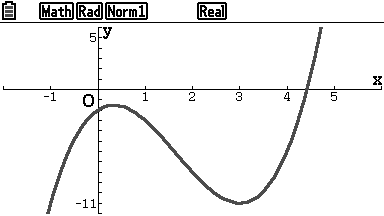
\includegraphics[scale=0.55]{assets/26-graph6.png}
          \end{vwcol}

          \begin{multicols}{2}
              \item $y = x^3 - 3x^2 + 4$
              \sol{}

              When $y = 0$,
              \begin{flalign*}
                  x^3 - 3x^2 + 4      & = 0               & \\
                  (x+1)(x^2 - 4x + 4) & = 0               & \\
                  (x+1)(x-2)^2        & = 0               & \\
                  x = -1              & \text{ or } x = 2
              \end{flalign*}
              $\therefore$ The $x$-intercepts are $(-1, 0)$ and $(2, 0)$.

              When $x = 0$, $y = 4$.

              $\therefore$ The $y$-intercept is $(0, 4)$.
              \begin{flalign*}
                  y'    & = 3x^2 - 6x       & \\
                  y''   & = 6x - 6          & \\
                  0     & = 3x^2 - 6x       & \\
                  0     & = x(x - 2)        & \\
                  x = 0 & \text{ or } x = 2
              \end{flalign*}
              When $x = 0$, $y'' = -6 < 0$.

              When $x = 2$, $y'' = 6 > 0$.

              $\therefore$ The function has a relative maximum point at $(0, 4)$ and a relative minimum point at $(2, 0)$.
              \begin{flalign*}
                  6x - 6 & = 0 & \\
                  x      & = 1
              \end{flalign*}
              When $x = 1$, $y = (1)^3 - 3(1)^2 + 4 = 2$.

              \noindent In the interval $(-\infty, 1)$, $y'' < 0$, hence the function is convex upward.

              \noindent In the interval $(1, \infty)$, $y'' > 0$, hence the function is convex downward.

              \noindent The point of inflection is $(1, 2)$.
              \vspace{2em}
              \begin{center}
                  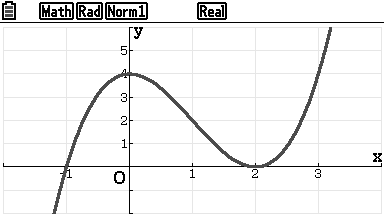
\includegraphics[scale=0.55]{assets/26-graph7.png}
              \end{center}
              \columnbreak

              \item In a container, the relationship between the volume of water $V$ (cm$^3$) and
              the depth of water $x$ (cm) is given by the equation $V = 4x^2 +
                  \dfrac{1}{6}x^3$. If the water is poured into the container at a rate of $6$
              cm$^3$ per second, find the rate of change of the depth of water when $x=2$ cm.
              \sol{}
              \begin{flalign*}
                  V              & = 4x^2 + \dfrac{1}{6}x^3                         & \\
                  \dfrac{dV}{dx} & = 8x + \dfrac{1}{2}x^2                           & \\
                  \dfrac{dV}{dt} & = 6                                              & \\
                  \dfrac{dx}{dt} & = \dfrac{dx}{dV} \cdot \dfrac{dV}{dt}            & \\
                                 & = \dfrac{1}{\dfrac{dV}{dx}} \cdot \dfrac{dV}{dt} & \\
                                 & = \dfrac{1}{8x + \dfrac{1}{2}x^2} \cdot 6        & \\
                                 & = \dfrac{6}{8x + \dfrac{1}{2}x^2}
              \end{flalign*}
              When $x = 2$,
              \begin{flalign*}
                  \dfrac{dx}{dt} & = \dfrac{6}{8(2) + \dfrac{1}{2}(2)^2} & \\
                                 & = \dfrac{6}{18}                       & \\
                                 & = \dfrac{1}{3} \text{ cm s}^{-1}
              \end{flalign*}
          \end{multicols}

          \newpage
    \item The water is poured into a conical pool with a height and a base radius of
          $20$m and $10$m respectively at a rate of $5$m$^3$/min. When the height of the
          water is $10$m, find
          \begin{enumerate}
              \item the rate of increasing of the height of the water. \sol{}

                    Let the height of the water be $h$cm and the radius of the water surface be
                    $r$cm.
                    \begin{flalign*}
                        \dfrac{h}{20}  & = \dfrac{r}{10}                                  & \\
                        r              & = \dfrac{h}{2}                                   & \\
                        V              & = \dfrac{1}{3}\pi r^2 h                          & \\
                                       & = \dfrac{1}{3}\pi \left(\dfrac{h}{2}\right)^2 h  & \\
                                       & = \dfrac{1}{12}\pi h^3                           & \\
                        \dfrac{dV}{dh} & = \dfrac{1}{4}\pi h^2                            & \\
                        \dfrac{dV}{dt} & = 5                                              & \\
                        \dfrac{dh}{dt} & = \dfrac{dh}{dV} \cdot \dfrac{dV}{dt}            & \\
                                       & = \dfrac{1}{\dfrac{dV}{dh}} \cdot \dfrac{dV}{dt} & \\
                                       & = \dfrac{1}{\dfrac{1}{4}\pi h^2} \cdot 5         & \\
                                       & = \dfrac{20}{\pi h^2} \text{ m min}^{-1}
                    \end{flalign*}
                    When $h = 10$,
                    \begin{flalign*}
                        \dfrac{dh}{dt} & = \dfrac{20}{\pi (10)^2}             & \\
                                       & = \dfrac{1}{5\pi} \text{ m min}^{-1}
                    \end{flalign*}

              \item the rate of change of the area of the water surface. \sol{}
                    \begin{flalign*}
                        A              & = \pi r^2                         & \\
                                       & = \pi \left(\dfrac{h}{2}\right)^2 & \\
                                       & = \dfrac{1}{4}\pi h^2             & \\
                        \dfrac{dA}{dh} & = \dfrac{1}{2}\pi h
                    \end{flalign*}
                    When $h = 10$,
                    \begin{flalign*}
                        \dfrac{dh}{dt} & = \dfrac{1}{5\pi}                            & \\
                        \dfrac{dA}{dt} & = \dfrac{dA}{dh} \cdot \dfrac{dh}{dt}        & \\
                                       & = \dfrac{1}{2}\pi (10) \cdot \dfrac{1}{5\pi} & \\
                                       & = 1 \text{ m}^2 \text{ min}^{-1}
                    \end{flalign*}
          \end{enumerate}

    \item The radius of a spherical container decreases from $4$cm to $3.95$cm. Find the
          approximate amount of decrease in the volume and the surface area of the
          container. \sol{}
          \begin{flalign*}
              V                          & = \dfrac{4}{3}\pi r^3     & \\
              A                          & = 4\pi r^2                & \\
              \dfrac{dV}{dr}             & = 4\pi r^2                & \\
              \dfrac{dA}{dr}             & = 8\pi r                  & \\
              \dfrac{\Delta V}{\Delta r} & = \dfrac{dV}{dr}          & \\
              \Delta V                   & = 4\pi r^2 \cdot \Delta r & \\
              \dfrac{\Delta A}{\Delta r} & = \dfrac{dA}{dr}          & \\
              \Delta A                   & = 8\pi r \cdot \Delta r
          \end{flalign*}
          When $r = 4$,$\Delta r = -0.05$,
          \begin{flalign*}
              \Delta V & = 4\pi (4)^2 (-0.05)   & \\
                       & = -3.2\pi \text{ cm}^3 & \\
              \Delta A & = 8\pi (4)(-0.05)      & \\
                       & = -1.6\pi \text{ cm}^2
          \end{flalign*}
          $\therefore$ The approximate amount of decrease in the volume and the surface area of the container is $-3.2\pi$cm$^3$ and $-1.6\pi$cm$^2$ respectively.
          \vfill\null

    \item The capacity of water of a spherical container is given by $V =
              \left[\dfrac{\pi h^2}{3}(15-h)\right]$cm$^3$, where $h$ is the depth of the
          water. Find the approximate amount of increase in the capacity of the container
          when the depth of the water increases from $4$cm to $4.01$cm. \sol{}
          \begin{flalign*}
              V                          & = 5\pi h^2 - \dfrac{1}{3}\pi h^3     & \\
              \dfrac{dV}{dh}             & = 10\pi h - \pi h^2                  & \\
              \dfrac{\Delta V}{\Delta h} & = \dfrac{dV}{dh}                     & \\
              \Delta V                   & = (10\pi h - \pi h^2) \cdot \Delta h &
          \end{flalign*}
          When $h = 4$,$\Delta h = 0.01$,
          \begin{flalign*}
              \Delta V & = (10\pi (4) - \pi (4)^2) \cdot 0.01 & \\
                       & = 0.24\pi \text{ cm}^3
          \end{flalign*}
          $\therefore$ The approximate amount of increase in the capacity of the container is $0.24\pi$cm$^3$.
          \vfill\null

          \newpage

    \item In a bowl, when the height of the water is $h$cm, the volume of the water is
          given by $V = \left(h^3 + 3h^2 + 11h\right)$cm$^3$. When the height of the
          water is $7cm$, pour an additional $\Delta V$cm$^3$ of water into the bowl.
          Find the approximate amount of increase in the height of the water. \sol{}
          \begin{flalign*}
              \dfrac{dV}{dh}             & = 3h^2 + 6h + 11                   & \\
              \dfrac{\Delta V}{\Delta h} & = \dfrac{dV}{dh}                   & \\
              \Delta V                   & = (3h^2 + 6h + 11) \cdot \Delta h  & \\
              \Delta h                   & = \dfrac{\Delta V}{3h^2 + 6h + 11}
          \end{flalign*}
          When $h = 7$,
          \begin{flalign*}
              \Delta h & = \dfrac{\Delta V}{3(7)^2 + 6(7) + 11} & \\
                       & = \dfrac{\Delta V}{200} \text{ cm}
          \end{flalign*}
          $\therefore$ The approximate amount of increase in the height of the water is $\dfrac{\Delta V}{200}$cm.

    \item If $y = \dfrac{1}{\sqrt[3]{x}}$, find $\dfrac{dy}{dx}$. Hence, find the
          approximate value of $\dfrac{1} {\sqrt[3]{130}}$. (Correct to 3 decimal places)
          \sol{}
          \begin{flalign*}
              y                          & = x^{-\frac{1}{3}}                             & \\
              \dfrac{dy}{dx}             & = -\dfrac{1}{3}x^{-\frac{4}{3}}                & \\
              \dfrac{\Delta y}{\Delta x} & = \dfrac{dy}{dx}                               & \\
              \Delta y                   & = -\dfrac{1}{3}x^{-\frac{4}{3}} \cdot \Delta x
          \end{flalign*}
          When $x = 125$, $\Delta x = 5$,
          \begin{flalign*}
              \Delta y & = -\dfrac{1}{3}(125)^{-\frac{4}{3}} \cdot 5 & \\
                       & = -0.003
          \end{flalign*}
          $\therefore$ The approximate value of $\dfrac{1} {\sqrt[3]{130}}$ is $\dfrac{1}{5} - 0.003 = 0.197$.
\end{enumerate}


\chapter{Indefinite Integrals}

\section{Indefinite Integrals as the Inverse of Differentiation}

Let function $F(x)$ and $f(x)$ be defined at the interval $(a, b)$. If any
point $x$ in this interval satisfies $F'(x) = f(x)$, then $F(x)$ is is the
preimage of $f(x)$ at the interval $(a, b)$.

According to the definition above, to find the preimage of a function $f(x)$,
we need to find the function $F(x)$ that satisfies $F'(x) = f(x)$. For example,
\begin{flalign*}
    (x^2)'     & = 2x   & \\
    (x^2 + 1)' & = 2x   & \\
    (x^2 - 2)' & = 2x   & \\
               & \vdots
\end{flalign*}

For any constant $C$, the derivative of $x^2 + C$ is $2x$. Hence, the preimage
of $2x$ is $x^2 + C$, where $C$ is an arbitary constant.

Since $\left[F(x) + C\right]' = F'(x) + 0 = F'(x)$, if the function $F(x)$ is a
preimage of $f(x)$, then $F(x) + C$ (C is a constant) is also a preimage of
$f(x)$. That is to say, there are infinite number of preimages of a function
$f(x)$.

In the other hand, if $F(x)$ and $G(x)$ are both preimages of $f(x)$, then
$F'(x) = f(x)$, $G'(x) = f(x)$.
\begin{flalign*}
    \because\ \left[G(x) - F(x)\right]' & = G'(x) - F'(x) & \\
                                        & = f(x) - f(x)   & \\
                                        & = 0
\end{flalign*}
\vspace{-3em}
\begin{flalign*}
    \therefore\ G(x) - F(x) & = C        & \\
    \text{i.e.}\ G(x)       & = F(x) + C
\end{flalign*}
This shows that for any two preimages of $f(x)$, the difference between them is a constant. If $F(x)$ is a preimage of $f(x)$, then all the preimages of $f(x)$ can be expressed as $F(x) + C$, where $C$ is a constant.
\subsection*{The Concept of Indefinite Integral}
Let function $F(x)$ be a preimage of $f(x)$. All the preimages $F(x) + C$ ($C$
is a constant) of a function $f(x)$ is called the indefinite integral of
$f(x)$, denoted by $\displaystyle\int f(x)dx$, i.e. $\displaystyle\int f(x)dx =
    F(x) + C$. $\displaystyle\int$ is called the integral sign, $f(x)$ is called
the integrand, $C$ is called the constant of integration.

Finding the indefinite integral of a function $f(x)$ is equivalent to finding
all the preimages of $f(x)$. From the explanation above, we just need to find
one preimage of $f(x)$, then add a constant $C$ to it to get the indefinite
integral of $f(x)$.

\section{Arithmetic Properties of Indefinite Integrals}

\subsection*{Basic Formulas of Indefinite Integrals}

In order to learn the methods and skills of finding indefinite integrals, we
must first learn some basic formulas of indefinite integrals. We know that
finding the indefinite integral is equivalent to finding the anti-derivative.
Therefore, we can get the formulas of indefinite integrals from the
corresponding formulas of derivatives.

For example, when $n \neq -1$, $\dfrac{d}{dx}\left(\dfrac{x^{n+1}}{n+1}\right)
    = x^n$.

Hence, $\displaystyle\int x^{n}dx = \dfrac{x^{n+1}}{n+1} + C$.

Similarly, we can also get the other basic formulas of indefinite integrals.
The basic formulas of indefinite integrals are listed below:
\begin{center}
    \framebox{
        \parbox[t][6cm]{12cm}{ \addvspace{0.2cm} \centering \begin{multicols}{2}
                \begin{enumerate}[label = ]
                    \item $\displaystyle\int x^{n}dx = \dfrac{x^{n+1}}{n+1} + C$, $n \neq -1$
                    \item $\displaystyle\int e^{x}dx = e^{x} + C$
                    \item $\displaystyle\int \sin xdx = -\cos x + C$
                    \item $\displaystyle\int \sec^2xdx = \tan x + C$
                    \item $\displaystyle\int \csc x\cot xdx = -\csc x + C$
                    \item $\displaystyle\int \dfrac{1}{x}dx = \ln|x| + C$
                    \item $\displaystyle\int a^{x}dx = \dfrac{a^x}{\ln a} + C$,
                    \item $\displaystyle\int \cos xdx = \sin x + C$
                    \item $\displaystyle\int \csc^2xdx = -\cot x + C$
                    \item $\displaystyle\int \sec x\tan xdx = \sec x + C$
                \end{enumerate}
            \end{multicols} }}
\end{center}
\vspace{0.9em}

\subsection{Practice 1}
\begin{enumerate}
      \item Find the equations of tangent and normal to the curve $y = x^3$ where $x = 2$.
            \sol{} \vspace{-1cm}
            \begin{multicols}{2}
                  \begin{flalign*}
                        y              & = x^3  & \\
                        \dfrac{dy}{dx} & = 3x^2
                  \end{flalign*}
                  At $x = 2$, $y = (2)^3 = 8$
                  \begin{flalign*}
                        \text{Gradient of tangent } \dfrac{dy}{dx} & = 3(2)^2 = 12    & \\
                        \text{Gradient of normal }                 & = -\dfrac{1}{12}
                  \end{flalign*}
                  \vfill\null
                  \begin{flalign*}
                        \therefore\ \text{Equation of tangent is } y - 8 & = 12(x - 2)             & \\
                        y                                                & = 12x - 16              & \\
                        \text{Equation of normal is } y - 8              & = -\dfrac{1}{12}(x - 2) & \\
                        12y - 96                                         & = -x + 2                & \\
                        x + 12y                                          & = 98                    & \\
                  \end{flalign*}
                  \vfill\null
            \end{multicols}
            \vspace{-1cm}

      \item Given that the gradient of tangent to the curve $y = x^2 - 2x + 3$ at point $Q$
            is $4$, find the coordinates of the point $Q$. \sol{}
            \begin{flalign*}
                  y              & = x^2 - 2x + 3 & \\
                  \dfrac{dy}{dx} & = 2x - 2
            \end{flalign*}
            At point $Q$, $\dfrac{dy}{dx} = 4$
            \begin{flalign*}
                  4 & = 2x - 2             & \\
                  x & = 3                  & \\
                  y & = 3^2 - 2(3) + 3 = 6
            \end{flalign*}
            $\therefore$ Coordinates of point $Q$ is $(3, 6)$.
            \vfill\null

      \item Find the equations of the tangent and normal to the curve $x^3 - 2xy + y^2 = 1$
            at point $(1, 2)$. \sol{}
            \begin{flalign*}
                  x^3 - 2xy + y^2                                 & = 1                          & \\
                  3x^2 - 2y - 2x\dfrac{dy}{dx} + 2y\dfrac{dy}{dx} & = 0                          & \\
                  (2x - 2y) \dfrac{dy}{dx}                        & = 3x^2 - 2y                  & \\
                  \dfrac{dy}{dx}                                  & = \dfrac{3x^2 - 2y}{2x - 2y}
            \end{flalign*}
            At point $(1, 2)$,
            \begin{flalign*}
                  \text{Gradient of tangent } \dfrac{dy}{dx} & = \dfrac{3(1)^2 - 2(2)}{2(1) - 2(2)} & \\
                                                             & = \dfrac{1}{2}                       & \\
                  \text{Gradient of normal }                 & = -2
            \end{flalign*}
            \begin{flalign*}
                  \therefore\ \text{Equation of tangent is } y - 2 & = \dfrac{1}{2}(x - 1) & \\
                  2y - 4                                           & = x - 1               & \\
                  x - 2y                                           & = -3                  & \\
                  \text{Equation of normal is } y - 2              & = -2(x - 1)           & \\
                  y - 2                                            & = -2x + 2             & \\
                  y                                                & = -2x + 4
            \end{flalign*}
            \vfill\null
\end{enumerate}
\subsection{Exercise 27.2a}
Find the following indefinite integrals:
\begin{enumerate}
    \begin{multicols}{2}
        \item $\displaystyle\int3xdx$
        \sol{}
        \begin{flalign*}
            I & = \dfrac{3}{2}x^2 + C &
        \end{flalign*}
        \item $\displaystyle\int5x^{4}dx$
        \sol{}
        \begin{flalign*}
            I & = x^5 + C &
        \end{flalign*}
    \end{multicols}

    \begin{multicols}{2}
        \item $\displaystyle\int5dx$
        \sol{}
        \begin{flalign*}
            I & = 5x + C &
        \end{flalign*}
        \item $\displaystyle\int x^{-9}dx$
        \sol{}
        \begin{flalign*}
            I & = -\dfrac{1}{8}x^{-8} + C &
        \end{flalign*}
    \end{multicols}

    \begin{multicols}{2}
        \item $\displaystyle\int x^{\frac{1}{2}}dx$
        \sol{}
        \begin{flalign*}
            I & = \dfrac{2}{3}x^{\frac{3}{2}} + C &
        \end{flalign*}
        \vfill{}\null{}
        \item $\displaystyle\int{2x^{-{\frac{1}{2}}}dx}$
        \sol{}
        \begin{flalign*}
            I & = 4x^{\frac{1}{2}} + C &
        \end{flalign*}
        \vfill{}\null{}
    \end{multicols}
    \vspace{-3em}

    \begin{multicols}{2}
        \item $\displaystyle\int{\dfrac{1}{x^5}}dx$
        \sol{}
        \begin{flalign*}
            I & = -\dfrac{1}{4}x^{-4} + C &
        \end{flalign*}
        \item $\displaystyle\int{\left(\dfrac{1}{x}\right)}^{4}dx$
        \sol{}
        \begin{flalign*}
            I & = -\dfrac{1}{3}x^{-3} + C &
        \end{flalign*}
    \end{multicols}

    \begin{multicols}{2}
        \item $\displaystyle\int{\sqrt{3x}}dx$
        \sol{}
        \begin{flalign*}
            I & = \int{\sqrt{3}\sqrt{x}}dx                & \\
              & = \sqrt{3}\int{\sqrt{x}}dx                & \\
              & = \dfrac{2\sqrt{3}}{3}x^{\frac{3}{2}} + C & \\
              & = \dfrac{2}{\sqrt{3}}x^{\frac{3}{2}} + C
        \end{flalign*}

        \item $\displaystyle\int{x^3\sqrt[3]{x^2}}dx$
        \sol{}
        \begin{flalign*}
            I & = \int{x^3x^{\frac{2}{3}}}dx        & \\
              & = \int{x^{\frac{11}{3}}}dx          & \\
              & = \dfrac{3}{14}x^{\frac{14}{3}} + C
        \end{flalign*}
    \end{multicols}

    \begin{multicols}{2}
        \item $\displaystyle\int{\cos(-x)}dx$
        \sol{}
        \begin{flalign*}
            I & = \int{\cos x}dx & \\
              & = \sin x + C
        \end{flalign*}

        \item $\displaystyle\int{\dfrac{2}{\csc x}}dx$
        \sol{}
        \begin{flalign*}
            I & = \int{2\sin x}dx & \\
              & = -2\cos x + C
        \end{flalign*}
    \end{multicols}

    \newpage

    \begin{multicols}{2}
        \item $\displaystyle\int{\dfrac{1}{\sin^2x}}dx$
        \sol{}
        \begin{flalign*}
            I & = \int{\csc^2x}dx & \\
              & = -\cot x + C
        \end{flalign*}
        \vfill{}\null{}

        \item $\displaystyle\int{\dfrac{1}{1 - \sin^2x}}dx$
        \sol{}
        \begin{flalign*}
            I & = \int{\dfrac{1}{\cos^2x}}dx & \\
              & = \int{\sec^2x}dx            & \\
              & = \tan x + C
        \end{flalign*}
    \end{multicols}

    \begin{multicols}{2}
        \item $\displaystyle\int{\dfrac{\sin x}{\cos^2x}}dx$
        \sol{}
        \begin{flalign*}
            I & = \int{\dfrac{\sin x}{\cos x}\cdot\dfrac{1}{\cos x}}dx & \\
              & = \int{\tan x\sec x}dx                                 & \\
              & = \sec x + C
        \end{flalign*}

        \item $\displaystyle\int{\dfrac{\cos x}{\sin^2x}}dx$
        \sol{}
        \begin{flalign*}
            I & = \int{\dfrac{\cos x}{\sin x}\cdot\dfrac{1}{\sin x}}dx & \\
              & = \int{\cot x\csc x}dx                                 & \\
              & = -\csc x + C
        \end{flalign*}
    \end{multicols}
\end{enumerate}

Using the arithmetic properties of derivatives, we can also get the following
arithmetic properties of indefinite integrals:
\begin{center}
    \framebox{
        \parbox[t][2.6cm]{12cm}{ \addvspace{0.2cm} \centering \begin{enumerate}
                \item Constant Multiple Rule: $\displaystyle\int kf(x)dx = k\int f(x)dx$, where $k$
                      is a constant.
                \item Sum and Difference Rule: $\displaystyle\int \left[f(x) \pm g(x)\right]dx = \int
                          f(x)dx \pm \int g(x)dx$
            \end{enumerate} }}
\end{center}
\vspace{0.9em}

Note that when integrating by parts, the result of each part of the integral
contains a constant of integration. However, the sum (or difference) of
multiple constants of integration is still a constant of integration.
Therefore, when integrating by parts, we only need to add one constant of
integration to the final result.

\subsection{Practice 2}

\begin{enumerate}
    \begin{multicols}{2}
        \item $\displaystyle\int_2^8 x d x$
        \sol{}
        \begin{flalign*}
            I & = \left[\dfrac{1}{2}x^2\right]_2^8 & \\
              & = \dfrac{1}{2}(64 - 4)             & \\
              & = 30
        \end{flalign*}

        \item $\displaystyle\int_{-2}^4 x^3 d x$
        \sol{}
        \begin{flalign*}
            I & = \left[\dfrac{1}{4}x^4\right]_{-2}^4 & \\
              & = \dfrac{1}{4}(256 - 16)              & \\
              & = 60
        \end{flalign*}
    \end{multicols}
    \begin{multicols}{2}
        \item $\displaystyle\int_{-\pi}^\pi \cos x d x$
        \sol{}
        \begin{flalign*}
            I & = \bigg[\sin x\bigg]_{-\pi}^\pi & \\
              & = \sin\pi - \sin(-\pi)          & \\
              & = 0 - 0                         & \\
              & = 0
        \end{flalign*}

        \item $\displaystyle\int_0^{\frac{\pi}{4}} \sec ^2 x d x$
        \sol{}
        \begin{flalign*}
            I & = \bigg[\tan x\bigg]_0^{\frac{\pi}{4}} & \\
              & = \tan\dfrac{\pi}{4} - \tan 0          & \\
              & = 1 - 0                                & \\
              & = 1
        \end{flalign*}
    \end{multicols}
\end{enumerate}

\newpage
\subsection{Practice 3}

\noindent \hspace{1.2em}\textit{
    Find the extreme values of the following functions (Question 1 to 4):
}

\begin{enumerate}
    \item $f(x)=x^2+x-6$
    \item $f(x)=2-x-x^2$
    \item $f(x)=\dfrac{1}{3} x^3-\dfrac{1}{2} x^2-2x+2$
    \item $f(x)=4 x-3 x^3$
\end{enumerate}

\noindent \hspace{1.2em}\textit{Find the coordinates of the extreme points of the following functions (Question 5 to 6):}
\begin{enumerate}[resume]
    \item $y=2 x^3-3 x^2-12 x-7$
    \item $y=x+\dfrac{1}{x}$
\end{enumerate}


\subsection{Exercise 27.2b}
Find the following indefinite integrals (Question 1 to 20):
\begin{enumerate}
    \begin{multicols}{2}
        \item $\displaystyle\int(x^3 - 3x + 1)dx$
        \sol{}
        \begin{flalign*}
            I & = \int x^3dx - \int 3xdx + \int dx          & \\
              & = \dfrac{1}{4}x^4 - \dfrac{3}{2}x^2 + x + C
        \end{flalign*}

        \item $\displaystyle\int\left(5x^4 + 2\sqrt{x}\right)dx$
        \sol{}
        \begin{flalign*}
            I & = \int 5x^4dx + \int 2\sqrt{x}dx        & \\
              & = x^5 + \dfrac{4}{3}x^{\frac{3}{2}} + C
        \end{flalign*}
    \end{multicols}

    \begin{multicols}{2}
        \item $\displaystyle\int\left({\dfrac{x^{2}}{2}}-{\dfrac{2}{x^{2}}}\right)dx$
        \sol{}
        \begin{flalign*}
            I & = \int{\dfrac{x^{2}}{2}}dx - \int{\dfrac{2}{x^{2}}}dx & \\
              & = \dfrac{1}{6}x^{3} + \dfrac{2}{x} + C
        \end{flalign*}
        \vfill{}\null{}

        \item $\displaystyle\int(\sin x-3\cos x)dx$
        \sol{}
        \begin{flalign*}
            I & = \int\sin xdx - \int3\cos xdx & \\
              & = -\cos x - 3\sin x + C
        \end{flalign*}
        \vfill{}\null{}
    \end{multicols}
    \vspace{-4em}
    \begin{multicols}{2}
        \item $\displaystyle\int(x-5)^2dx$
        \sol{}
        \begin{flalign*}
            I & = \int(x^2 - 10x + 25)dx           & \\
              & = \dfrac{1}{3}x^3 - 5x^2 + 25x + C
        \end{flalign*}

        \item $\displaystyle\int(x-1)(x-2)dx$
        \sol{}
        \begin{flalign*}
            I & = \int(x^2 - 3x + 2)dx                       & \\
              & = \dfrac{1}{3}x^3 - \dfrac{3}{2}x^2 + 2x + C
        \end{flalign*}
    \end{multicols}

    \begin{multicols}{2}
        \item $\displaystyle\int(x^2 + 2)\sqrt{x}dx$
        \sol{}
        \begin{flalign*}
            I & = \int x^{\frac{5}{2}}dx + \int 2x^{\frac{1}{2}}dx              & \\
              & = \dfrac{2}{7}x^{\frac{7}{2}} + \dfrac{4}{3}x^{\frac{3}{2}} + C
        \end{flalign*}

        \item $\displaystyle\int\dfrac{x^4 - 5}{x^2}dx$
        \sol{}
        \begin{flalign*}
            I & = \int x^2dx - \int\dfrac{5}{x^2}dx  & \\
              & = \dfrac{1}{3}x^3 + \dfrac{5}{x} + C
        \end{flalign*}
    \end{multicols}

    \begin{multicols}{2}
        \item $\displaystyle\int\dfrac{x+5}{\sqrt{x}}dx$
        \sol{}
        \begin{flalign*}
            I & = \int x^{\frac{1}{2}}dx + \int 5x^{-\frac{1}{2}}dx   & \\
              & = \dfrac{2}{3}x^{\frac{3}{2}} + 10x^{\frac{1}{2}} + C
        \end{flalign*}
        \vfill{}\null{}

        \item $\displaystyle\int\dfrac{\sqrt[3]{x^2} - \sqrt[4]{x}}{\sqrt{x}}dx$
        \sol{}
        \begin{flalign*}
            I & = \int \dfrac{x^{\frac{2}{3}} - x^{\frac{1}{4}}}{x^{\frac{1}{2}}}dx & \\
              & = \int \left(x^{\frac{1}{6}} - x^{-\frac{1}{4}}\right)dx            & \\
              & = \dfrac{6}{7}x^{\frac{7}{6}} - \dfrac{4}{3}x^{\frac{3}{4}} + C
        \end{flalign*}
    \end{multicols}

    \begin{multicols}{2}
        \item $\displaystyle\int\dfrac{x^2 - 9}{x + 3}dx$
        \sol{}
        \begin{flalign*}
            I & = \int \dfrac{(x + 3)(x - 3)}{x + 3}dx & \\
              & = \int (x - 3)dx                       & \\
              & = \dfrac{1}{2}x^2 - 3x + C
        \end{flalign*}

        \item $\displaystyle\int\dfrac{x^3 - 8}{x - 2}dx$
        \sol{}
        \begin{flalign*}
            I & = \int \dfrac{(x - 2)(x^2 + 2x + 4)}{x - 2}dx & \\
              & = \int (x^2 + 2x + 4)dx                       & \\
              & = \dfrac{1}{3}x^3 + x^2 + 4x + C
        \end{flalign*}
    \end{multicols}

    \begin{multicols}{2}
        \item $\displaystyle\int\sqrt[3]{x^2}\left(\sqrt{x} - \dfrac{1}{x}\right)dx$
        \sol{}
        \begin{flalign*}
            I & = \int x^{\frac{2}{3}}\left(x^{\frac{1}{2}} - x^{-1}\right)dx     & \\
              & = \int \left(x^{\frac{7}{6}} - x^{-\frac{1}{3}}\right)dx          & \\
              & = \dfrac{6}{13}x^{\frac{13}{6}} - \dfrac{3}{2}x^{\frac{2}{3}} + C
        \end{flalign*}

        \item $\displaystyle\int\dfrac{(2x + 1)^2}{x}dx$
        \sol{}
        \begin{flalign*}
            I & = \int\dfrac{4x^2 + 4x + 1}{x}dx            & \\
              & = \int \left(4x + 4 + \dfrac{1}{x}\right)dx & \\
              & = 2x^2 + 4x + \ln|x| + C
        \end{flalign*}
    \end{multicols}

    \begin{multicols}{2}
        \item $\displaystyle\int\dfrac{(x + 1)(3x^2 - 4)}{2x^3}dx$
        \sol{}
        \begin{flalign*}
            I & = \int\dfrac{3x^3 + 3x^2 - 4x - 4}{2x^3}dx                                          & \\
              & = \int\left(\dfrac{3}{2} + \dfrac{3}{2x} - \dfrac{2}{x^2} - \dfrac{2}{x^3}\right)dx & \\
              & = \dfrac{3}{2}x - \dfrac{3}{2}\ln|x| + \dfrac{2}{x} + \dfrac{1}{x^2} + C
        \end{flalign*}
        \vfill{}\null{}

        \item $\displaystyle\int\left(\dfrac{x - 1}{x^2}\right)^2dx$
        \sol{}
        \begin{flalign*}
            I & = \int\left(\dfrac{x^2 - 2x + 1}{x^4}\right)dx         & \\
              & = \int\left(x^{-2} - 2x^{-3} + x^{-4}\right)dx         & \\
              & = -x^{-1} + x^{-2} - \dfrac{1}{3}x^{-3} + C            & \\
              & = -\dfrac{1}{x} + \dfrac{1}{x^2} - \dfrac{1}{3x^3} + C
        \end{flalign*}
    \end{multicols}

    \begin{multicols}{2}
        \item $\displaystyle\int\left(\sin\dfrac{x}{2} - \cos\dfrac{x}{2}\right)^2dx$
        \sol{}
        \begin{flalign*}
            I & = \int\left(\sin^2\dfrac{x}{2} - 2\sin\dfrac{x}{2}\cos\dfrac{x}{2} + \cos^2\dfrac{x}{2}\right)dx & \\
              & = \int\left(1 - \sin x\right)dx = x + \cos x + C
        \end{flalign*}
        \vfill{}\null{}

        \item $\displaystyle\int\tan^2xdx$
        \sol{}
        \begin{flalign*}
            I & = \int(\sec^2x - 1)dx & \\
              & = \tan x - x + C
        \end{flalign*}
        \vfill{}\null{}
    \end{multicols}
    \vspace{-3em}

    \begin{multicols}{2}
        \item $\displaystyle\int\left(e^2 + \dfrac{1}{4x}\right)dx$
        \sol{}
        \begin{flalign*}
            I & = \int e^2dx + \dfrac{1}{4}\int\dfrac{1}{x}dx & \\
              & = e^2x + \dfrac{1}{4}\ln|x| + C
        \end{flalign*}

        \item $\displaystyle\int(2e)^xdx$
        \sol{}
        \begin{flalign*}
            I & = \dfrac{(2e)^x}{\ln(2e)} + C   & \\
              & = \dfrac{(2e)^x}{\ln 2 + 1} + C
        \end{flalign*}
    \end{multicols}

    \begin{multicols}{2}
        \item Given the function $y = \dfrac{5x}{3 - x}$, find $\dfrac{dy}{dx}$. Hence,
        \\find $\displaystyle\int\dfrac{1}{(3 - x)^2}dx$. \sol{}
        \begin{flalign*}
            \dfrac{dy}{dx}             & = \dfrac{5(3 - x) - 5x(-1)}{(3 - x)^2}          & \\
                                       & = \dfrac{15}{(3 - x)^2}                         & \\
                                       &                                                   \\
            \int\dfrac{1}{(3 - x)^2}dx & = \int\dfrac{1}{15}\cdot\dfrac{15}{(3 - x)^2}dx & \\
                                       & = \dfrac{1}{15}\int\dfrac{15}{(3 - x)^2}dx      & \\
                                       & = \dfrac{1}{15}\int\dfrac{dy}{dx}dx             & \\
                                       & = \dfrac{1}{15}y + C                            & \\
                                       & = \dfrac{1}{15}\cdot\dfrac{5x}{3 - x} + C       & \\
                                       & = \dfrac{x}{3(3 - x)} + C
        \end{flalign*}

        \item If the function $y = \dfrac{2x^2}{3x - 1}$, find $\dfrac{dy}{dx}$. Hence,
        \\find $\displaystyle\int\dfrac{2x - 3x^2}{(3x - 1)^2}dx$. \sol{}
        \begin{flalign*}
            \dfrac{dy}{dx}                      & = \dfrac{2(3x - 1)(2x) - 2x^2(3)}{(3x - 1)^2}     & \\
                                                & = \dfrac{12x^2 - 4x - 6x^2}{(3x - 1)^2}           & \\
                                                & = \dfrac{6x^2 - 4x}{(3x - 1)^2}                   & \\
                                                &                                                     \\
            \int\dfrac{2x - 3x^2}{(3x - 1)^2}dx & = -dfrac{1}{2}\int\dfrac{6x^2 - 4x}{(3x - 1)^2}dx & \\
                                                & = -\dfrac{1}{2}\int\dfrac{dy}{dx}dx               & \\
                                                & = -\dfrac{1}{2}y + C                              & \\
                                                & = -\dfrac{1}{2}\cdot\dfrac{2x^2}{3x - 1} + C      & \\
                                                & = -\dfrac{x^2}{3x - 1} + C
        \end{flalign*}
    \end{multicols}

    \item Prove that $\dfrac{d}{dx}\left(\dfrac{3x^2}{x^2 + 2}\right) = \dfrac{12x}{(x^2
                  + 2)^2}$. Hence, find $\displaystyle\int\dfrac{4x}{(x^2 + 2)^2}dx$. \sol{}
          \begin{flalign*}
              \dfrac{d}{dx}\left(\dfrac{3x^2}{x^2 + 2}\right) & = \dfrac{(x^2 + 2)(6x) - (3x^2)(2x)}{(x^2 + 2)^2} & \\
                                                              & = \dfrac{6x^3 + 12x - 6x^3}{(x^2 + 2)^2}          & \\
                                                              & = \dfrac{12x}{(x^2 + 2)^2} \qquad \blacksquare
          \end{flalign*}
          \newpage{}

    \item Given that ${\dfrac{d}{dx}}{\left(\dfrac{3x^{2}-1}{5x^{2}+7}\right)}=f(x)$,
          find $\displaystyle\int\left[3x^2 - 1 - 2f(x)\right]dx$. \sol{}
          \begin{flalign*}
              \int\left[3x^2 - 1 - 2f(x)\right]dx & = \int3x^2dx - \int dx - 2\int f(x)dx            & \\
                                                  & = x^3 - x - 2\cdot\dfrac{3x^2 - 1}{5x^2 + 7} + C & \\
                                                  & = x^3 - x - \dfrac{6x^2 - 2}{5x^2 + 7} + C
          \end{flalign*}

    \item Given that ${\dfrac{d}{dx}}\left({\dfrac{2+x^{3}}{2-x^{3}}}\right)=3g(x)$, find
          $\displaystyle\int\left[g(x) - 3x + 2\right]dx$. \sol{}
          \begin{flalign*}
              \int\left[g(x) - 3x + 2\right]dx & = \int g(x)dx - 3\int xdx + 2\int dx                                           & \\
                                               & = \int g(x)dx - \dfrac{3}{2}x^2 + 2x + C                                       & \\
                                               & = \int\dfrac{1}{3}\cdot3g(x)dx - \dfrac{3}{2}x^2 + 2x + C                      & \\
                                               & = \dfrac{1}{3}\left(\dfrac{2 + x^3}{2 - x^3}\right) - \dfrac{3}{2}x^2 + 2x + C & \\
                                               & = \dfrac{2 + x^3}{3(2 - x^3)} - \dfrac{3}{2}x^2 + 2x + C
          \end{flalign*}
\end{enumerate}

\section{Integration by Substitution}

In the last section, we learned to find the indefinite integral of some
functions using some basic formulas of indefinite integrals and two arithmetic
properties of indefinite integrals. However, for the indefinite integral of
some more complicated functions like $\displaystyle\int 3\sqrt{3x + 1}dx$,
$\displaystyle\int 2\sin2xdx$, etc., we cannot find their indefinite integrals
straight away using the basic formulas of indefinite integrals and the
arithmetic properties of indefinite integrals. Hence, we need to learn some
other methods to find the indefinite integral of these functions. Here we will
introduce a method called integration by substitution.

Consider a function $F(u)$, where $u$ is a function of $x$, i.e. $u = g(x)$.

Using the chain rule, we have $\dfrac{d}{dx}F\left(g(x)\right) =
    F'\left(g(x)\right) \cdot g'(x)$. Hence,
\begin{center}
    \framebox{
        \parbox[t][1.2cm]{6cm}{ \addvspace{0.2cm} \centering $\displaystyle\int
                F'\left(g(x)\right) \cdot g'(x)dx = F\left(g(x)\right) + C$ }}
\end{center}
\vspace{0.9em}
Generally speaking, during the calculation process, we let $u = g(x)$.
\begin{flalign*}
    \therefore\ \displaystyle\int F'\left(g(x)\right) \cdot g'(x)dx & = \int F'(u)\dfrac{du}{dx}dx & \\
                                                                    & = \int F'(u)du               & \\
                                                                    & = F(u) + C                   & \\
                                                                    & = F\left(g(x)\right) + C
\end{flalign*}
For the functions that we cannot find their indefinite integrals straight away using the basic formulas of indefinite integrals, if it can be expressed in the form of $\displaystyle\int F'\left(g(x)\right) \cdot g'(x)dx$, we can perform substitution using $u = g(x)$ and express the indefinite integral as $\displaystyle\int F'(u)du$ to find its indefinite integral.

\subsection{Practice 4}

\noindent \hspace{1.2em}\textit{Find the absolute maximum value and the absolute minimum value of the following functions (Question 1 to 2):}
\begin{enumerate}
    \item $f(x) = 3x^3 - 9x + 5$, $[-2, 2]$
    \item $f(x) = x^4 - 2x^2 + 5$, $[-2, 3]$
    \item If $x + y = 8$, find the absolute minimum value of $x^2 + y^2$.
    \item A metal wire with a length of $100$cm is bent into a rectangle. Find the width
          and the length of the rectangle so that the area of the rectangle is the
          largest.
\end{enumerate}
\subsection{Exercise 27.3a}
\noindent \hspace{1.2em}\textit{Find the following indefinite integral:}
\begin{enumerate}
    \begin{multicols}{2}
        \item $\displaystyle\int(2x+1)^{3} dx$
        \sol{}

        Let $u = 2x + 1$, $du = 2dx$.
        \begin{flalign*}
            I & = \dfrac{1}{2}\int u^{3}du              & \\
              & = \dfrac{1}{2}\cdot\dfrac{u^{4}}{4} + C & \\
              & = \dfrac{1}{8}(2x + 1)^{4} + C
        \end{flalign*}

        \item $\displaystyle\int(3x+2)^{5} dx$
        \sol{}

        Let $u = 3x + 2$, $du = 3dx$.
        \begin{flalign*}
            I & = \dfrac{1}{3}\int u^{5}du              & \\
              & = \dfrac{1}{3}\cdot\dfrac{u^{6}}{6} + C & \\
              & = \dfrac{1}{18}(3x + 2)^{6} + C
        \end{flalign*}
    \end{multicols}

    \begin{multicols}{2}
        \item $\displaystyle\int(3-x)^{6} dx$
        \sol{}

        Let $u = 3 - x$, $du = -dx$.
        \begin{flalign*}
            I & = -\int u^{6}du                                       & \\
              & = -\dfrac{u^{7}}{7} + C = -\dfrac{(3 - x)^{7}}{7} + C
        \end{flalign*}

        \item $\displaystyle\int(2x-1)^{-3} dx$
        \sol{}

        Let $u = 2x - 1$, $du = 2dx$.
        \begin{flalign*}
            I & = \dfrac{1}{2}\int u^{-3}du                                               & \\
              & = \dfrac{1}{2}\cdot\dfrac{u^{-2}}{-2} + C = -\dfrac{1}{4(2x - 1)^{2}} + C
        \end{flalign*}
    \end{multicols}

    \begin{multicols}{2}
        \item $\displaystyle\int4{\sqrt{2x-1}} dx$
        \sol{}

        Let $u = 2x - 1$, $du = 2dx$.
        \begin{flalign*}
            I & = 2\int{\sqrt{u}}du                      & \\
              & = 2\cdot\dfrac{2}{3}u^{\frac{3}{2}} + C  & \\
              & = \dfrac{4}{3}(2x - 1)^{\frac{3}{2}} + C
        \end{flalign*}

        \item $\displaystyle\int2(3x+1)^{2} dx$
        \sol{}

        Let $u = 3x + 1$, $du = 3dx$.
        \begin{flalign*}
            I & = \dfrac{2}{3}\int u^{2}du              & \\
              & = \dfrac{2}{3}\cdot\dfrac{u^{3}}{3} + C & \\
              & = \dfrac{2}{9}(3x + 1)^{3} + C
        \end{flalign*}
    \end{multicols}

    \begin{multicols}{2}
        \item $\displaystyle\int\dfrac{dx}{(2x+5)^{8}}$
        \sol{}

        Let $u = 2x + 5$, $du = 2dx$.
        \begin{flalign*}
            I & = \dfrac{1}{2}\int u^{-8}du               & \\
              & = \dfrac{1}{2}\cdot\dfrac{u^{-7}}{-7} + C & \\
              & = -\dfrac{1}{14(2x + 5)^{7}} + C
        \end{flalign*}

        \item $\displaystyle\int\dfrac{2}{(3-2x)^{2}} dx$
        \sol{}

        Let $u = 3 - 2x$, $du = -2dx$.
        \begin{flalign*}
            I & = -\int\dfrac{1}{u^{2}}du & \\
              & = \dfrac{1}{u} + C        & \\
              & = \dfrac{1}{3 - 2x} + C
        \end{flalign*}
    \end{multicols}

    \begin{multicols}{2}
        \item $\displaystyle\int x{\sqrt{x^{2}+1}} dx$
        \sol{}

        Let $u = x^2 + 1$, $du = 2xdx$.
        \begin{flalign*}
            I & = \dfrac{1}{2}\int{\sqrt{u}}du                     & \\
              & = \dfrac{1}{2}\cdot\dfrac{2}{3}u^{\frac{3}{2}} + C & \\
              & = \dfrac{1}{3}(x^2 + 1)^{\frac{3}{2}} + C
        \end{flalign*}

        \item $\displaystyle\int 3x^{2}\left(x^{3}+4\right)^{3} dx$
        \sol{}

        Let $u = x^3 + 4$, $du = 3x^2dx$.
        \begin{flalign*}
            I & = \int u^{3}du                  & \\
              & = \dfrac{u^{4}}{4} + C          & \\
              & = \dfrac{1}{4}(x^3 + 4)^{4} + C
        \end{flalign*}
    \end{multicols}

    \begin{multicols}{2}
        \item $\displaystyle\int15x^{2}\left(x^{3}-1\right)^{4} dx$
        \sol{}

        Let $u = x^3 - 1$, $du = 3x^2dx$.
        \begin{flalign*}
            I \int15x^{2}\le & = \int 5u^{4}du         & \\
                             & = \dfrac{5u^{5}}{5} + C & \\
                             & = u^{5} + C             & \\
                             & = (x^3 - 1)^{5} + C
        \end{flalign*}

        \item $\displaystyle\int\left(2x+1\right)\!\left(x^{2}+x\!+\!2\right)^{5} dx$
        \sol{}

        Let $u = x^2 + x + 2$, $du = (2x + 1)dx$.
        \begin{flalign*}
            I & = \int u^{5}du                      & \\
              & = \dfrac{u^{6}}{6} + C              & \\
              & = \dfrac{1}{6}(x^2 + x + 2)^{6} + C
        \end{flalign*}
    \end{multicols}

    \newpage
    \begin{multicols}{2}
        \item $\displaystyle\int\left(x^{2}-2x\right)\left(x^{3}-3x^{2}+1\right)^{4} dx$
        \sol{}

        Let $u = x^3 - 3x^2 + 1$, $du = (3x^2 - 6x)dx$.
        \begin{flalign*}
            I & = \int u^{4}du                         & \\
              & = \dfrac{u^{5}}{5} + C                 & \\
              & = \dfrac{1}{5}(x^3 - 3x^2 + 1)^{5} + C
        \end{flalign*}

        \item $\displaystyle\int\dfrac{x+1}{{{x}^{2}}+2x+3} dx$
        \sol{}

        Let $u = x^2 + 2x + 3$, $du = (2x + 2)dx = 2(x + 1)dx$.
        \begin{flalign*}
            I & = \dfrac{1}{2}\int\dfrac{1}{u}du    & \\
              & = \dfrac{1}{2}\ln|u| + C            & \\
              & = \dfrac{1}{2}\ln|x^2 + 2x + 3| + C
        \end{flalign*}

    \end{multicols}
    \begin{multicols}{2}
        \item $\displaystyle\int x^{2}\cos\left(x^{3}+2\right) dx$
        \sol{}

        Let $u = x^3 + 2$, $du = 3x^2dx$.
        \begin{flalign*}
            I & = \dfrac{1}{3}\int\cos udu      & \\
              & = \dfrac{1}{3}\sin u + C        & \\
              & = \dfrac{1}{3}\sin(x^3 + 2) + C
        \end{flalign*}

        \item $\displaystyle\int\sin{\dfrac{x}{2}} dx$
        \sol{}

        Let $u = \dfrac{x}{2}$, $du = \dfrac{1}{2}dx$.
        \begin{flalign*}
            I & = 2\int\sin udu            & \\
              & = -2\cos u + C             & \\
              & = -2\cos{\dfrac{x}{2}} + C
        \end{flalign*}

    \end{multicols}
    \begin{multicols}{2}
        \item $\displaystyle\int\dfrac{\ln^2 x}{x} dx$
        \sol{}

        Let $u = \ln x$, $du = \dfrac{1}{x}dx$.
        \begin{flalign*}
            I & = \int u^2du              & \\
              & = \dfrac{u^3}{3} + C      & \\
              & = \dfrac{1}{3}\ln^3 x + C
        \end{flalign*}

        \item $\displaystyle\int e^{1 - 2x} dx$
        \sol{}

        Let $u = 1 - 2x$, $du = -2dx$.
        \begin{flalign*}
            I & = -\dfrac{1}{2}\int e^udu     & \\
              & = -\dfrac{1}{2}e^u + C        & \\
              & = -\dfrac{1}{2}e^{1 - 2x} + C
        \end{flalign*}

    \end{multicols}
    \begin{multicols}{2}
        \item $\displaystyle\int\left(e^{x}+e^{-x}\right) dx$
        \sol{}

        Let $u = -x$, $du = -dx$.
        \begin{flalign*}
            I & = \int e^x dx - \int e^u du & \\
              & = e^x - e^u + C             & \\
              & = e^x - e^{-x} + C
        \end{flalign*}

        \item $\displaystyle\int x e^{x^2} dx$
        \sol{}

        Let $u = x^2$, $du = 2xdx$.
        \begin{flalign*}
            I & = \dfrac{1}{2}\int e^u du & \\
              & = \dfrac{1}{2}e^u + C     & \\
              & = \dfrac{1}{2}e^{x^2} + C
        \end{flalign*}
    \end{multicols}

\end{enumerate}

\newpage
\subsection{Practice 5}
Find the following indefinite integral:
\begin{enumerate}
    \begin{multicols}{2}
        \item $\displaystyle\int\sin2x\cos2x dx$
        \sol{}
        \begin{flalign*}
            I & = \dfrac{1}{2}\int\sin4x dx & \\
              & = -\dfrac{1}{8}\cos4x + C
        \end{flalign*}
        \vfill{}\null{}

        \item $\displaystyle\int\cos^2 2x dx$
        \sol{}
        \begin{flalign*}
            I & = \int\dfrac{1 + \cos 4x}{2} dx                    & \\
              & = \dfrac{1}{2}\int dx + \dfrac{1}{2}\int\cos 4x dx & \\
              & = \dfrac{1}{2}x + \dfrac{1}{8}\sin 4x + C
        \end{flalign*}
    \end{multicols}
    \begin{multicols}{2}
        \item $\displaystyle\int\sin^3 x dx$
        \sol{}
        \begin{flalign*}
            I & = \int\sin^2 x\sin x dx                 & \\
              & = \int(1 - \cos^2 x)\sin x dx           & \\
              & = \int\sin x dx - \int\cos^2 x\sin x dx
        \end{flalign*}
        Let $u = \cos x$, $du = -\sin xdx$.
        \begin{flalign*}
            I & = -\int \cos x dx + \int u^2 du    & \\
              & = -\sin x + \dfrac{1}{3}u^3 + C    & \\
              & = \dfrac{1}{3}\cos^3 x -\sin x + C
        \end{flalign*}

        \item $\displaystyle\int\cos^3 x dx$
        \sol{}
        \begin{flalign*}
            I & = \int\cos^2 x\cos x dx                 & \\
              & = \int(1 - \sin^2 x)\cos x dx           & \\
              & = \int\cos x dx - \int\sin^2 x\cos x dx
        \end{flalign*}
        Let $u = \sin x$, $du = \cos xdx$.
        \begin{flalign*}
            I & = \int \cos x dx - \int u^2 du      & \\
              & = \sin x - \dfrac{1}{3}u^3 + C      & \\
              & = \sin x - \dfrac{1}{3}\sin^3 x + C
        \end{flalign*}
    \end{multicols}
    \begin{multicols}{2}
        \item $\displaystyle\int\tan^4 x\sec^2 x dx$
        \sol{}

        Let $u = \tan x$, $du = \sec^2 xdx$.
        \begin{flalign*}
            I & = \int u^4 du              & \\
              & = \dfrac{u^5}{5} + C       & \\
              & = \dfrac{1}{5}\tan^5 x + C
        \end{flalign*}
        \vfill{}\null{}
        \columnbreak
        \item $\displaystyle\int\tan^4\dfrac{x}{2} dx$
        \sol{}
        \begin{flalign*}
            I & = \int\tan^2\dfrac{x}{2}\tan^2\dfrac{x}{2} dx                             & \\
              & = \int\left(\sec^2\dfrac{x}{2} - 1\right)\tan^2\dfrac{x}{2} dx            & \\
              & = \int\sec^2\dfrac{x}{2}\tan^2\dfrac{x}{2} dx - \int\tan^2\dfrac{x}{2} dx
        \end{flalign*}
        Let $u = \tan\dfrac{x}{2}$, $du = \dfrac{1}{2}\sec^2\dfrac{x}{2}dx$.
        \begin{flalign*}
            I & = 2\int u^2 du - \int \tan^2\dfrac{x}{2} dx                     & \\
              & = \dfrac{2u^3}{3} - \int \left(\sec^2\dfrac{x}{2} - 1\right) dx & \\
              & = \dfrac{2u^3}{3} - \int \sec^2\dfrac{x}{2} dx + \int dx        & \\
              & = \dfrac{2}{3}\tan^3\dfrac{x}{2} - 2\tan\dfrac{x}{2} + x + C
        \end{flalign*}
    \end{multicols}
\end{enumerate}
\subsection{Exercise 27.3b}
\noindent \hspace{1.2em}\textit{Find the following indefinite integral:}
\begin{enumerate}
    \begin{multicols}{2}
        \item $\displaystyle\int\sin^2\dfrac{x}{2} dx$
        \sol{}
        \begin{flalign*}
            I & = \int\left(\dfrac{1 - \cos x}{2}\right) dx       & \\
              & = \dfrac{1}{2}\int dx - \dfrac{1}{2}\int\cos x dx & \\
              & = \dfrac{1}{2}x - \dfrac{1}{2}\sin x + C
        \end{flalign*}
        \vfill{}\null{}

        \item $\displaystyle\int\tan^2 5x dx$
        \sol{}
        \begin{flalign*}
            I & = \int\left(\sec^2 5x - 1\right) dx        & \\
              & = \int\sec^2 5x dx - \int dx               & \\
              & = \dfrac{1}{5}\int\sec^2 5xd(5x) - \int dx & \\
              & = \dfrac{1}{5}\tan 5x - x + C
        \end{flalign*}
    \end{multicols}

    \begin{multicols}{2}
        \item $\displaystyle\int\dfrac{1}{\sec^2 4x} dx$
        \sol{}
        \begin{flalign*}
            I & = \int\cos^2 4x dx                                 & \\
              & = \int\dfrac{1 + \cos 8x}{2} dx                    & \\
              & = \dfrac{1}{2}\int dx + \dfrac{1}{2}\int\cos 8x dx & \\
              & = \dfrac{1}{16}\sin 8x + \dfrac{1}{2}x + C
        \end{flalign*}

        \item $\displaystyle\int\cos^2(3x - 1) dx$
        \sol{}
        \begin{flalign*}
            I & = \int\left(\dfrac{1 + \cos 2(3x - 1)}{2}\right) dx      & \\
              & = \dfrac{1}{2}\int dx + \dfrac{1}{2}\int\cos (6x - 2) dx & \\
              & = \dfrac{1}{12}\sin (6x - 2) + \dfrac{1}{2}x + C
        \end{flalign*}
    \end{multicols}

    \begin{multicols}{2}
        \item $\displaystyle\int\sec5x\tan5x dx$
        \sol{}
        \begin{flalign*}
            I & = \dfrac{1}{5}\int\sec5x\tan5x d(5x) & \\
              & = \dfrac{1}{5}\sec5x + C
        \end{flalign*}

        \item $\displaystyle\int-\csc3x\cot3x dx$
        \sol{}
        \begin{flalign*}
            I & = \dfrac{1}{3}\int-\csc3x\cot3x d(3x) & \\
              & = \dfrac{1}{3}\csc3x + C
        \end{flalign*}
    \end{multicols}

    \begin{multicols}{2}
        \item $\displaystyle\int\left(\sin\dfrac{x}{8} - \sec^2 2x\right) dx$
        \sol{}
        \begin{flalign*}
            I & = \int\sin\dfrac{x}{8} dx - \int\sec^2 2x dx                                           & \\
              & = -8\int\sin \dfrac{x}{8} d\left(\dfrac{x}{8}\right) - \dfrac{1}{2}\int\sec^2 2x d(2x) & \\
              & = -8\cos\dfrac{x}{8} - \dfrac{1}{2}\tan 2x + C
        \end{flalign*}
        \vfill{}\null{}
        \columnbreak{}

        \item $\displaystyle\int\left(\sin{\dfrac{x}{2}}+\cos{\dfrac{x}{2}}\right)^{2} dx$
        \sol{}

        Let $u = \dfrac{x}{2}$, $du = \dfrac{1}{2}dx$.
        \begin{flalign*}
            I & = 2\int\left(\sin u + \cos u\right)^2 du                   & \\
              & = 2\int\left(\sin^2 u + 2\sin u\cos u + \cos^2 u\right) du & \\
              & = 2\int\left(1 + \sin 2u\right) du                         & \\
              & = 2\left(u - \dfrac{1}{2}\cos 2u\right) + C                & \\
              & = x - \cos x + C
        \end{flalign*}
    \end{multicols}

    \begin{multicols}{2}
        \item $\displaystyle\int(\sec x+\tan x)^{2} dx$
        \sol{}
        \begin{flalign*}
            I & = \int(\sec^2 x + 2\sec x\tan x + \tan^2 x) dx                   & \\
              & = \int\sec^2 x + 2\int\sec x\tan x dx + \int\tan^2 x dx          & \\
              & = \int\sec^2 x dx + 2\int\sec x\tan x dx + \int(\sec^2 x - 1) dx & \\
              & = \tan x + 2\sec x + \tan x - x + C                              & \\
              & = 2\tan x + 2\sec x - x + C
        \end{flalign*}

        \item $\displaystyle\int(2-\sin x)^{2} dx$
        \sol{}
        \begin{flalign*}
            I & = \int(4 - 4\sin x + \sin^2 x) dx                                               & \\
              & = \int 4 dx - 4\int\sin x dx + \dfrac{1}{2}\int(1 - \cos 2x) dx                 & \\
              & = \int 4 dx - 4\int\sin x dx + \dfrac{1}{2}\int dx - \dfrac{1}{2}\int\cos 2x dx & \\
              & = 4x + 4\cos x + \dfrac{1}{2}x - \dfrac{1}{4}\sin 2x + C                        & \\
              & = \dfrac{9}{2}x + 4\cos x - \dfrac{1}{4}\sin 2x + C
        \end{flalign*}
    \end{multicols}

    \begin{multicols}{2}
        \item $\displaystyle\int\cos^4 x dx$
        \sol{}
        \begin{flalign*}
            I & = \int\cos^2 x\cos^2 x dx                                                                         & \\
              & = \int(1 - \sin^2 x)\cos^2 x dx                                                                   & \\
              & = \int\cos^2 x dx - \int\sin^2 x\cos^2 x dx                                                       & \\
              & = \int\dfrac{1 + \cos 2x}{2} dx - \int\dfrac{1 - \cos 2x}{2}\cdot\dfrac{1 + \cos 2x}{2} dx        & \\
              & = \dfrac{1}{2}\int dx + \dfrac{1}{2}\int\cos 2x dx - \dfrac{1}{4}\int(1 - \cos^2 2x) dx           & \\
              & = \dfrac{1}{2}\int dx + \dfrac{1}{2}\int\cos 2x dx - \dfrac{1}{4}\int dx                          & \\
              & \ \ \ \ + \dfrac{1}{4}\int\dfrac{1 + \cos 4x}{2} dx                                               & \\
              & = \dfrac{1}{2}\int dx + \dfrac{1}{2}\int\cos 2x dx - \dfrac{1}{4}\int dx + \dfrac{1}{8}\int dx    & \\
              & \ \ \ \ + \dfrac{1}{8}\int\cos 4x dx                                                              & \\
              & = \dfrac{1}{2}x + \dfrac{1}{4}\sin 2x - \dfrac{1}{4}x + \dfrac{1}{16}x + \dfrac{1}{32}\sin 4x + C & \\
              & = \dfrac{3}{8}x + \dfrac{1}{4}\sin 2x + \dfrac{1}{32}\sin 4x + C
        \end{flalign*}

        \item $\displaystyle\int\left(1+\tan^{2}x\right)\left(1-\tan^{2}x\right) dx$
        \sol{}
        \begin{flalign*}
            I & = \int\left(1 - \tan^4 x\right) dx                              & \\
              & = \int dx - \int\tan^4 x dx                                     & \\
              & = \int dx - \int(\sec^2 x - 1)\tan^2 x dx                       & \\
              & = \int dx - \int\sec^2 x\tan^2 x dx + \int\tan^2 x dx           & \\
              & = \int dx - \int\sec^2 x\tan^2 x dx + \int(\sec^2 x - 1)dx      & \\
              & = \int dx - \int\sec^2 x\tan^2 x dx + \int\sec^2 x dx - \int dx & \\
              & = \int\sec^2 x dx - \int\sec^2 x\tan^2 x dx
        \end{flalign*}
        Let $u = \tan x$, $du = \sec^2 xdx$.
        \begin{flalign*}
            I & = \int\sec ^{2}x dx - \int u^{2}du  & \\
              & = \tan x - \dfrac{u^{3}}{3} + C     & \\
              & = \tan x - \dfrac{\tan^{3}x}{3} + C
        \end{flalign*}
    \end{multicols}

    \begin{multicols}{2}
        \item $\displaystyle\int\sin^{2}4x\cos4x dx$
        \sol{}

        Let $u = \sin 4x$, $du = 4\cos 4x dx$.
        \begin{flalign*}
            I & = \dfrac{1}{4}\int u^2 du             & \\
              & = \dfrac{1}{4}\cdot\dfrac{u^3}{3} + C & \\
              & = \dfrac{1}{12}\sin^3 4x + C
        \end{flalign*}

        \item $\displaystyle\int3\cot^{3}3x\csc^{2}3x dx$
        \sol{}

        Let $u = \cot 3x$, $du = -3\csc^2 3x dx$.
        \begin{flalign*}
            I & = -\int u^3 du               & \\
              & = -\dfrac{u^4}{4} + C        & \\
              & = -\dfrac{1}{4}\cot^4 3x + C
        \end{flalign*}
    \end{multicols}

    \begin{multicols}{2}
        \item $\displaystyle\int\tan^{2}x\sec^{4}x dx$
        \sol{}
        \begin{flalign*}
            I & = \int\tan^{2}x(\tan^2 x + 1)\sec^2 x dx            & \\
              & = \int\tan^4 x\sec^2 x dx + \int\tan^2 x\sec^2 x dx
        \end{flalign*}
        Let $u = \tan x$, $du = \sec^2 xdx$.
        \begin{flalign*}
            I & = \int u^4 du + \int u^2 du                       & \\
              & = \dfrac{u^5}{5} + \dfrac{u^3}{3} + C             & \\
              & = \dfrac{1}{5}\tan^5 x + \dfrac{1}{3}\tan^3 x + C
        \end{flalign*}

        \item $\displaystyle\int\sec x\cdot\tan^{3}x dx$
        \sol{}
        \begin{flalign*}
            I & = \int\sec x\cdot(\sec^2 x - 1)\tan x dx      & \\
              & = \int\sec^3 x\tan x dx - \int\sec x\tan x dx
        \end{flalign*}
        Let $u = \sec x$, $du = \sec x\tan xdx$.
        \begin{flalign*}
            I & = \int u^2 du - \int \sec x\tan xdx & \\
              & = \dfrac{u^3}{3} - \sec x + C       & \\
              & = \dfrac{1}{3}\sec^3 x - \sec x + C
        \end{flalign*}
    \end{multicols}
\end{enumerate}

\section{Integration by Partial Fractions}

Generally speaking, in order to find the indefinite integral of a proper
fraction, we first have to decompose the proper fraction into partial
fractions, then perform integration on each term. This method of integration is
called integration by partial fractions.

To find the partial fractions of an improper fraction, we can first decompose
the fraction into the sum of a polynomial and a proper fraction using
polynomial division.

\subsection{Practice 6}

Sketch the graph of the function $f(x) = x^3 - 3x^2 + 2$.

\newpage

\subsection{Exercise 27.4}

\noindent \hspace{1.2em}\textit{Find the following indefinite integral:}
\begin{enumerate}
    \begin{multicols}{2}
        \item $\displaystyle\int\dfrac{1}{x(x+1)} dx$
        \sol{}

        Let $\dfrac{1}{x(x+1)} = \dfrac{A}{x} + \dfrac{B}{x+1}$.
        \begin{flalign*}
            \dfrac{1}{x(x+1)} & = \dfrac{A}{x} + \dfrac{B}{x+1} & \\
            1                 & = Ax + A + Bx                   & \\
                              & = (A + B)x + A
        \end{flalign*}
        \vspace{-2em}
        \begin{flalign*}
            \begin{cases}
                A + B = 0 \\
                A = 1
            \end{cases}
            \Rightarrow
            \begin{cases}
                A = 1 \\
                B = -1
            \end{cases}
        \end{flalign*}
        \vspace{-1em}
        \begin{flalign*}
            I & = \int\left(\dfrac{1}{x} - \dfrac{1}{x+1}\right) dx & \\
              & = \ln|x| - \ln|x+1| + C
        \end{flalign*}

        \item $\displaystyle\int\dfrac{x}{(x+1)(x-3)} dx$
        \sol{}

        Let $\dfrac{x}{(x+1)(x-3)} = \dfrac{A}{x+1} + \dfrac{B}{x-3}$.
        \begin{flalign*}
            \dfrac{x}{(x+1)(x-3)} & = \dfrac{A}{x+1} + \dfrac{B}{x-3} & \\
            x                     & = Ax - 3A + Bx + B                & \\
                                  & = (A + B)x + (-3A + B)
        \end{flalign*}
        \vspace{-2em}
        \begin{flalign*}
            \begin{cases}
                A + B = 1 \\
                -3A + B = 0
            \end{cases}
            \Rightarrow
            \begin{cases}
                A = \dfrac{1}{4} \\
                B = \dfrac{3}{4}
            \end{cases}
        \end{flalign*}
        \vspace{-1em}
        \begin{flalign*}
            I & = \int\left(\dfrac{1}{4}\cdot\dfrac{1}{x+1} + \dfrac{3}{4}\cdot\dfrac{1}{x-3}\right) dx & \\
              & = \dfrac{1}{4}\ln|x+1| + \dfrac{3}{4}\ln|x-3| + C
        \end{flalign*}
    \end{multicols}

    \begin{multicols}{2}
        \item $\displaystyle\int\dfrac{4x-13}{2x^2+x-6} dx$
        \sol{}

        Let $\dfrac{4x-13}{2x^2+x-6} = \dfrac{A}{2x-3} + \dfrac{B}{x+2}$.
        \begin{flalign*}
            \dfrac{4x-13}{2x^2+x-6} & = \dfrac{A}{2x-3} + \dfrac{B}{x+2} & \\
            4x - 13                 & = Ax + 2A + 2Bx - 3B               & \\
                                    & = (A + 2B)x + (2A - 3B)
        \end{flalign*}
        \vspace{-2em}
        \begin{flalign*}
            \begin{cases}
                A + 2B = 4 \\
                2A - 3B = -13
            \end{cases}
            \Rightarrow
            \begin{cases}
                A = -2 \\
                B = 3
            \end{cases}
        \end{flalign*}
        \vspace{-1em}
        \begin{flalign*}
            I & = \int\left(\dfrac{-2}{2x-3} + \dfrac{3}{x+2}\right) dx & \\
              & = 3\ln|x+2| -\ln|2x-3|+ C
        \end{flalign*}

        \item $\displaystyle\int\dfrac{5x-1}{1-x^{2}} dx$
        \sol{}

        Let $\dfrac{5x-1}{1-x^{2}} = \dfrac{A}{1-x} + \dfrac{B}{1+x}$.
        \begin{flalign*}
            \dfrac{5x-1}{1-x^{2}} & = \dfrac{A}{1-x} + \dfrac{B}{1+x} & \\
            5x - 1                & = A + Ax + B - Bx                 & \\
                                  & = (A - B)x + (A + B)
        \end{flalign*}
        \vspace{-2em}
        \begin{flalign*}
            \begin{cases}
                A - B = 5 \\
                A + B = -1
            \end{cases}
            \Rightarrow
            \begin{cases}
                A = 2 \\
                B = -3
            \end{cases}
        \end{flalign*}
        \vspace{-1em}
        \begin{flalign*}
            I & = \int\left(\dfrac{2}{1-x} - \dfrac{3}{1+x}\right) dx & \\
              & = -2\ln|1-x| - 3\ln|1+x| + C
        \end{flalign*}
    \end{multicols}

    \newpage

    \begin{multicols}{2}
        \item $\displaystyle\int\dfrac{x^{2}+5}{(x+1)(x-1)} dx$
        \sol{}
        \begin{flalign*}
            I & = \int\dfrac{x^{2}+5}{x^2 - 1}               & \\
              & = \int\left(1 + \dfrac{6}{x^2 - 1}\right) dx
        \end{flalign*}
        Let $\dfrac{6}{x^2 - 1} = \dfrac{A}{x-1} + \dfrac{B}{x+1}$.
        \begin{flalign*}
            \dfrac{6}{x^2 - 1} & = \dfrac{A}{x-1} + \dfrac{B}{x+1} & \\
            6                  & = Ax + A + Bx - B                 & \\
                               & = (A + B)x + (A - B)
        \end{flalign*}
        \vspace{-2em}
        \begin{flalign*}
            \begin{cases}
                A + B = 0 \\
                A - B = 6
            \end{cases}
            \Rightarrow
            \begin{cases}
                A = 3 \\
                B = -3
            \end{cases}
        \end{flalign*}
        \vspace{-1em}
        \begin{flalign*}
            I & = \int\left(1 + \dfrac{3}{x-1} - \dfrac{3}{x+1}\right) dx & \\
              & = x + 3\ln|x-1| - 3\ln|x+1| + C
        \end{flalign*}

        \item $\displaystyle\int\dfrac{x^{3}+2}{x^{2}-1} dx$
        \sol{}
        \begin{flalign*}
            I & = \int\dfrac{x^{3}+2}{x^{2}-1} dx                 & \\
              & = \int \left(x + \dfrac{x + 2}{x^{2}-1}\right) dx
        \end{flalign*}
        Let $\dfrac{x + 2}{x^{2}-1} = \dfrac{A}{x-1} + \dfrac{B}{x+1}$.
        \begin{flalign*}
            \dfrac{x + 2}{x^{2}-1} & = \dfrac{A}{x-1} + \dfrac{B}{x+1} & \\
            x + 2                  & = Ax + A + Bx - B                 & \\
                                   & = (A + B)x + (A - B)
        \end{flalign*}
        \vspace{-2em}
        \begin{flalign*}
            \begin{cases}
                A + B = 1 \\
                A - B = 2
            \end{cases}
            \Rightarrow
            \begin{cases}
                A = \dfrac{3}{2} \\
                B = -\dfrac{1}{2}
            \end{cases}
        \end{flalign*}
        \vspace{-1em}
        \begin{flalign*}
            I & = \int\left(x + \dfrac{3}{2}\cdot\dfrac{1}{x-1} - \dfrac{1}{2}\cdot\dfrac{1}{x+1}\right) dx & \\
              & = \dfrac{1}{2}x^2 + \dfrac{3}{2}\ln|x-1| - \dfrac{1}{2}\ln|x+1| + C
        \end{flalign*}
    \end{multicols}

    \begin{multicols}{2}
        \item $\displaystyle\int\dfrac{2x-1}{x^{2}+2x+1} dx$
        \sol{}
        \begin{flalign*}
            I & = \int\dfrac{2x-1}{(x+1)^2} dx
        \end{flalign*}
        Let $u = x + 1$, $du = dx$, $x = u - 1$.
        \begin{flalign*}
            I & = \int\dfrac{2u - 3}{u^2} du     & \\
              & = \int(2u^{-1} - 3u^{-2}) du     & \\
              & = 2\ln|u| + \dfrac{3}{u} + C     & \\
              & = 2\ln|x+1| + \dfrac{3}{x+1} + C
        \end{flalign*}

        \item $\displaystyle\int\dfrac{4x-3}{(2x+1)^{2}} dx$
        \sol{}

        Let $u = 2x + 1$, $du = 2dx$, $x = \dfrac{u - 1}{2}$.
        \begin{flalign*}
            I & = \dfrac{1}{2}\int\dfrac{2u - 5}{u^2}du  & \\
              & = \dfrac{1}{2}\int(2u^{-1} - 5u^{-2})du  & \\
              & = \ln|u| + \dfrac{5}{2u} + C             & \\
              & = \ln|2x + 1| + \dfrac{5}{2(2x + 1)} + C
        \end{flalign*}
    \end{multicols}
\end{enumerate}

\newpage
\section{Applications of Indefinite Integrals}

We can use derivative to find the slope of a tangent line to a curve at any
point on the curve. Conversely, if the slope of a tangent line to a curve at a
point on the curve is known, we can use indefinite integration to find the
equation of the curve.

\subsection{Practice 7}
\begin{enumerate}
      \begin{multicols}{2}
            \item A drop of ink gradually spread after being dropped onto a piece of paper. At
            $t$ seconds, its area is $A = \left(3t^2 + \dfrac{1}{5}t + 2\right)$mm$^2$.
            Find the rate of change of the ink spread at $t = 2$ second. \sol{}
            \begin{flalign*}
                  \dfrac{dA}{dt} & = 6t + \dfrac{1}{5}
            \end{flalign*}
            When $t = 2$,
            \begin{flalign*}
                  \dfrac{dA}{dt} & = 6(2) + \dfrac{1}{5}      \\
                                 & = 12 + \dfrac{1}{5}        \\
                                 & = \dfrac{61}{5}            \\
                                 & = 12.2\text{mm}^2\text{/s}
            \end{flalign*}
            \vfill\null

            \item The radius of a sphere increases at a rate of $3$cm/s. When the radius is
            $5$cm, find the rate of change of the surface area of the sphere. \sol{}
            \begin{flalign*}
                  \dfrac{dr}{dt} & = 3\text{cm/s}                      \\
                  A              & = 4\pi r^2                          \\
                  \dfrac{dA}{dr} & = 8\pi r                            \\
                  \dfrac{dA}{dt} & = \dfrac{dA}{dr}\cdot\dfrac{dr}{dt} \\
                                 & = 8\pi r\cdot 3\text{cm/s}          \\
                                 & = 24\pi r\text{cm}^2\text{/s}
            \end{flalign*}
            When $r = 5$,
            \begin{flalign*}
                  \dfrac{dA}{dt} & = 24\pi(5)\text{cm}^2\text{/s} \\
                                 & = 120\pi\text{cm}^2\text{/s}
            \end{flalign*}
      \end{multicols}
\end{enumerate}
\subsection{Exercise 27.5}

\begin{enumerate}
    \item Given that $\dfrac{dy}{dx} = 4x^3 - 6x^2 + 3$, and when $x = 2$, $y = 7$.
          Express $y$ in terms of $x$. \sol{}
          \begin{flalign*}
              \dfrac{dy}{dx} & = 4x^3 - 6x^2 + 3         & \\
              dy             & = (4x^3 - 6x^2 + 3)dx     & \\
              \int dy        & = \int(4x^3 - 6x^2 + 3)dx & \\
              y              & = x^4 - 2x^3 + 3x + C
          \end{flalign*}
          When $x = 2$, $y = 7$.
          \begin{flalign*}
              7 & = 16 - 16 + 6 + C & \\
              C & = 1
          \end{flalign*}
          $\therefore$ $y = x^4 - 2x^3 + 3x + 1$.
          \newpage
    \item The gradient of the tangent line of a point on a curve is $\dfrac{dy}{dx} = x^2
              + 2x - 4$, and the curve passes through point $(3, 3)$. Find the equation of
          the curve. \sol{}
          \begin{flalign*}
              \dfrac{dy}{dx} & = x^2 + 2x - 4                   & \\
              dy             & = (x^2 + 2x - 4)dx               & \\
              \int dy        & = \int(x^2 + 2x - 4)dx           & \\
              y              & = \dfrac{1}{3}x^3 + x^2 - 4x + C
          \end{flalign*}
          When $x = 3$, $y = 3$.
          \begin{flalign*}
              3 & = 9 + 9 - 12 + C & \\
              C & = -3
          \end{flalign*}
          $\therefore$ The equation of the curve is $y = \dfrac{1}{3}x^3 + x^2 - 4x - 3$.

    \item The gradient of a curve at the point $(1, -1)$ is $-4$, and $\dfrac{dy}{dx} =
              \sqrt{x} + k$. Find
          \begin{enumerate}
              \item The value of $k$. \sol{}

                    When $x = 1$, $\dfrac{dy}{dx} = -4$
                    \begin{flalign*}
                        -4 & = \sqrt{1} + k & \\
                        k  & = -5
                    \end{flalign*}

              \item The equation of the curve. \sol{}
                    \begin{flalign*}
                        \dfrac{dy}{dx} & = \sqrt{x} - 5                         & \\
                        dy             & = (\sqrt{x} - 5)dx                     & \\
                        \int dy        & = \int(\sqrt{x} - 5)dx                 & \\
                        y              & = \dfrac{2}{3}x^{\frac{3}{2}} - 5x + C
                    \end{flalign*}
                    When $x = 1$, $y = -1$.
                    \begin{flalign*}
                        -1 & = \dfrac{2}{3} - 5 + C & \\
                        C  & = \dfrac{10}{3}
                    \end{flalign*}
                    $\therefore$ The equation of the curve is $y = \dfrac{2}{3}x^{\frac{3}{2}} - 5x + \dfrac{10}{3}$.

          \end{enumerate}
\end{enumerate}

\newpage
\section{Revision Exercise 27}

Find the following indefinite integral (Question 1 to 34):
\begin{enumerate}
    \begin{multicols}{2}
        \item $\displaystyle\int 2x^{\frac{1}{5}}dx$
        \sol{}
        \begin{flalign*}
            I & = 2 \cdot \dfrac{5}{6}x^{\frac{6}{5}} + C & \\
              & = \dfrac{5}{3}x^{\frac{6}{5}} + C
        \end{flalign*}
        \vfill{}\null{}
        \item $\displaystyle\int{(2x-1)}^3dx$
        \sol{}
        \begin{flalign*}
            I & = \dfrac{1}{2}\int{(2x-1)}^3d(2x-1)             & \\
              & = \dfrac{1}{2} \cdot \dfrac{1}{4}{(2x-1)}^4 + C & \\
              & = \dfrac{1}{8}{(2x-1)}^4 + C
        \end{flalign*}
    \end{multicols}

    \begin{multicols}{2}
        \item $\displaystyle\int{(x+4)}^{100}dx$
        \sol{}
        \begin{flalign*}
            I & = \int{(x+4)}^{100}d(x+4)         & \\
              & = \dfrac{1}{101}{(x+4)}^{101} + C
        \end{flalign*}
        \item $\displaystyle\int{\left(\dfrac{5}{x^2}+2x^{\frac{1}{2}}+3\right)}dx$
        \sol{}
        \begin{flalign*}
            I & =5\int{x^{-2}} + 2\int{x^{\frac{1}{2}}} + 3\int dx     & \\
              & = -\dfrac{5}{x} + \dfrac{4}{3}x^{\frac{3}{2}} + 3x + C
        \end{flalign*}
    \end{multicols}

    \begin{multicols}{2}
        \item $\displaystyle\int{\left(3x^2 + \dfrac{1}{x^2} - \sin x\right)}dx$
        \sol{}
        \begin{flalign*}
            I & = 3\int x^2 + \int x^{-2} - \int \sin x dx & \\
              & = x^3 - x^{-1} + \cos x + C                & \\
              & = x^3 + \dfrac{1}{x} + \cos x + C
        \end{flalign*}
        \item $\displaystyle\int{\left(4\cos x + \dfrac{1}{x} + x^3\right)}dx$
        \sol{}
        \begin{flalign*}
            I & = 4\int \cos x + \int x^{-1} + \int x^3 dx          & \\
              & = 4\sin x + \ln \vert x \vert + \dfrac{1}{4}x^4 + C
        \end{flalign*}
    \end{multicols}

    \begin{multicols}{2}
        \item $\displaystyle\int\dfrac{3x^3 - 2x^2 + x^{-1}}{x^2}dx$
        \sol{}
        \begin{flalign*}
            I & = \int(3x - 2 + x^{-3})dx                       & \\
              & = \dfrac{3}{2}x^2 - 2x - \dfrac{1}{2}x^{-2} + C
        \end{flalign*}
        \item $\displaystyle\int(2x-1)(x+2)dx$
        \sol{}
        \begin{flalign*}
            I & = \int(2x^2 + 3x - 2)dx                      & \\
              & = \dfrac{2}{3}x^3 + \dfrac{3}{2}x^2 - 2x + C
        \end{flalign*}
    \end{multicols}

    \begin{multicols}{2}
        \item $\displaystyle\int{\left(x-\dfrac{1}{x^2}\right)}^2dx$
        \sol{}
        \begin{flalign*}
            I & = \int(x^2 - 2x^{-1} + x^{-4})dx                                & \\
              & = \dfrac{1}{3}x^3 - 2\ln \vert x \vert - \dfrac{1}{3}x^{-3} + C
        \end{flalign*}
        \item $\displaystyle\int{\left(x + \dfrac{1}{x}\right)}^3dx$
        \sol{}
        \begin{flalign*}
            I & = \int(x^3 + 3x + 3x^{-1} + x^{-3})dx                                             & \\
              & = \dfrac{1}{4}x^4 + \dfrac{3}{2}x^2 + 3\ln \vert x \vert - \dfrac{1}{2}x^{-2} + C
        \end{flalign*}
    \end{multicols}
    \newpage
    \begin{multicols}{2}
        \item $\displaystyle\int10^{-x}dx$
        \sol{}
        \begin{flalign*}
            I & = -\int10^{-x}d(-x)            & \\
              & = -\dfrac{10^{-x}}{\ln 10} + C & \\
              & = -\dfrac{1}{10^{x}\ln 10} + C
        \end{flalign*}
        \item $\displaystyle\int{\left(e^x - e^{-x}\right)}^2dx$
        \sol{}
        \begin{flalign*}
            I & = \int(e^{2x} - 2 + e^{-2x})dx                      & \\
              & = \dfrac{1}{2}e^{2x} - 2x - \dfrac{1}{2}e^{-2x} + C
        \end{flalign*}
    \end{multicols}

    \begin{multicols}{2}
        \item $\displaystyle\int2x{(x^2 - 1)}^4dx$
        \sol{}
        \begin{flalign*}
            I & = \int{(x^2 - 1)}^4d(x^2 - 1)   & \\
              & = \dfrac{1}{5}{(x^2 - 1)}^5 + C
        \end{flalign*}
        \item $\displaystyle\int3x^2{(x^3 + 1)}^4dx$
        \sol{}
        \begin{flalign*}
            I & = \int{(x^3 + 1)}^4d(x^3 + 1)   & \\
              & = \dfrac{1}{5}{(x^3 + 1)}^5 + C
        \end{flalign*}
    \end{multicols}

    \begin{multicols}{2}
        \item $\displaystyle\int\dfrac{x+1}{{(x^2 + 2x + 5)}^3}dx$
        \sol{}
        \begin{flalign*}
            I & = \dfrac{1}{2}\int\dfrac{1}{(x^2 + 2x + 5)^3}d(x^2 + 2x + 5) & \\
              & = -\dfrac{1}{4(x^2 + 2x + 5)^2} + C
        \end{flalign*}
        \item $\displaystyle\int\dfrac{2x}{\sqrt{x^2-4}}dx$
        \sol{}
        \begin{flalign*}
            I & = \int\dfrac{1}{\sqrt{x^2-4}}d(x^2-4) & \\
              & = 2\sqrt{x^2-4} + C
        \end{flalign*}
    \end{multicols}

    \begin{multicols}{2}
        \item $\displaystyle\int\dfrac{x-2}{\sqrt{(x-1)(x-3)}}dx$
        \sol{}
        \begin{flalign*}
            I & = \int\dfrac{x-2}{\sqrt{x^2-4x+3}}dx                    & \\
              & = \dfrac{1}{2}\int\dfrac{1}{\sqrt{x^2-4x+3}}d(x^2-4x+3) & \\
              & = \dfrac{1}{2}\cdot 2\sqrt{x^2-4x+3} + C                & \\
              & = \sqrt{x^2-4x+3} + C
        \end{flalign*}
        \vfill{}\null{}
        \columnbreak
        \item $\displaystyle\int\dfrac{7}{2x^2 + 5x - 3}dx$
        \sol{}
        \begin{flalign*}
            I = \int\dfrac{7}{(2x - 1)(x + 3)}dx &
        \end{flalign*}
        \vspace{-2em}
        \begin{flalign*}
            \text{Let } \dfrac{7}{(2x - 1)(x + 3)} & = \dfrac{A}{2x - 1} + \dfrac{B}{x + 3} & \\
            A(x + 3) + B(2x - 1)                   & = 7                                    & \\
            (A + 2B)x + (3A - B)                   & = 7
        \end{flalign*}
        Comparing coefficients,
        \begin{flalign*}
            A + 2B    & = 0  & \\
            3A - B    & = 7  & \\
            A = 2,\ B & = -1
        \end{flalign*}
        \vspace{-2em}
        \begin{flalign*}
            I & = \int\left(\dfrac{2}{2x-1} - \dfrac{1}{x + 3}\right)dx & \\
              & = \int\dfrac{2}{2x-1}dx - \int\dfrac{1}{x + 3}dx        & \\
              & = \ln|2x - 1| - \ln|x + 3| + C                          & \\
              & = \ln\left|\dfrac{2x - 1}{x + 3}\right| + C
        \end{flalign*}
    \end{multicols}

    \begin{multicols}{2}
        \item $\displaystyle\int\dfrac{8 - 7x}{2 + x - 3x^2}dx$
        \sol{}
        \begin{flalign*}
            I & = -\int\dfrac{7x + 8}{(3x + 2)(x - 1)}dx
        \end{flalign*}
        \vspace{-2em}
        \begin{flalign*}
            \text{Let } \dfrac{7x + 8}{(3x + 2)(x - 1)} & = \dfrac{A}{3x + 2} + \dfrac{B}{x - 1} & \\
            A(x - 1) + B(3x + 2)                        & = 7x + 8                               & \\
            (A + 3B)x + (-A + 2B)                       & = 7x + 8
        \end{flalign*}
        Comparing coefficients,
        \begin{flalign*}
            A + 3B     & = 7 & \\
            -A + 2B    & = 8 & \\
            A = -2,\ B & = 3
        \end{flalign*}
        \vspace{-2em}
        \begin{flalign*}
            I & = -\int\left(-\dfrac{2}{3x + 2} + \dfrac{3}{x - 1}\right)dx & \\
              & = -\int-\dfrac{2}{3x + 2}dx - \int\dfrac{3}{x - 1}dx        & \\
              & = \dfrac{2}{3}\ln|3x + 2| - 3\ln|x - 1| + C                 & \\
        \end{flalign*}
        \item $\displaystyle\int\dfrac{x+1}{(3x+2)(5x+3)}dx$
        \sol{}
        \vspace{-2em}
        \begin{flalign*}
            \text{Let } \dfrac{x+1}{(3x+2)(5x+3)} & = \dfrac{A}{3x+2} + \dfrac{B}{5x+3} & \\
            A(5x + 3) + B(3x + 2)                 & = x + 1                             & \\
            (5A + 3B)x + (3A + 2B)                & = x + 1
        \end{flalign*}
        Comparing coefficients,
        \begin{flalign*}
            5A + 3B    & = 1 & \\
            3A + 2B    & = 1 & \\
            A = -1,\ B & = 2
        \end{flalign*}
        \begin{flalign*}
            I & = \int\left(\dfrac{-1}{3x+2} + \dfrac{2}{5x+3}\right)dx  & \\
              & = -\int\dfrac{1}{3x+2}dx + \int\dfrac{2}{5x+3}dx         & \\
              & = -\dfrac{1}{3}\ln|3x + 2| + \dfrac{2}{5}\ln|5x + 3| + C & \\
        \end{flalign*}
    \end{multicols}

    \begin{multicols}{2}
        \item $\displaystyle\int\dfrac{2x^2 + 5x - 2}{2x^2 + x - 3}dx$
        \sol{}
        \begin{flalign*}
            I & = \int\left(1 + \dfrac{4x + 1}{2x^2 + x - 3}\right)dx          & \\
              & = \int\left[1 + \dfrac{(2x^2 + x - 3)'}{2x^2 + x - 3}\right]dx & \\
              & = x + \ln\vert2x^2 + x - 3\vert + C
        \end{flalign*}
        \item $\displaystyle\int{\left(\dfrac{x+1}{x-1}\right)}^2dx$
        \sol{}
        \begin{flalign*}
            I & = \int\left(1 + \dfrac{2}{x-1}\right)^2dx                    & \\
              & = \int\left[1 + \dfrac{4}{x-1} + \dfrac{4}{(x-1)^2}\right]dx & \\
              & = x + 4\ln\vert x - 1\vert - \dfrac{4}{x - 1} + C
        \end{flalign*}
    \end{multicols}

    \begin{multicols}{2}
        \item $\displaystyle\int\dfrac{{(x-1)}^3}{{(x-2)}^2}dx$
        \sol{}

        Let $u = x - 2$, $du = dx$.
        \begin{flalign*}
            I & = \int\dfrac{{(u+1)}^3}{u^2}du                                                &   & \\
              & = \int\left(\dfrac{u^3 + 3u^2 + 3u + 1}{u^2}\right)du                         &     \\
              & = \int\left(u + 3 + \dfrac{3}{u} + \dfrac{1}{u^2}\right)du                    &     \\
              & = \dfrac{u^2}{2} + 3u + 3\ln\vert u\vert - \dfrac{1}{u} + C                   &     \\
              & = \dfrac{x^2 - 4x + 4 + 6x - 12}{2} + 3\ln\vert x-2\vert - \dfrac{1}{x-2} + C &     \\
              & = \dfrac{1}{2}x^2 + x + 3\ln\vert x-2\vert - \dfrac{1}{x-2} + C
        \end{flalign*}
        \item $\displaystyle\int\dfrac{x^2}{{(x+2)}^3}dx$
        \sol{}

        Let $u = x + 2$, $du = dx$.
        \begin{flalign*}
            I & = \int\dfrac{{(u-2)}^2}{u^3}du                                      & \\
              & = \int\left(\dfrac{u^2 - 4u + 4}{u^3}\right)du                      & \\
              & = \int\left(\dfrac{1}{u} - \dfrac{4}{u^2} + \dfrac{4}{u^3}\right)du & \\
              & = \ln\vert u\vert + \dfrac{4}{u} - \dfrac{2}{u^2} + C               & \\
              & = \ln\vert x+2\vert + \dfrac{4}{x+2} - \dfrac{2}{(x+2)^2} + C
        \end{flalign*}
    \end{multicols}

    \begin{multicols}{2}
        \item $\displaystyle\int\left(3\sin2x-4e^{3x}\right)dx$
        \sol{}
        \begin{flalign*}
            I & = \dfrac{3}{2}\int\sin2xd(2x) - \int4e^{3x}dx  & \\
              & = -\dfrac{3}{2}\cos2x - \dfrac{4}{3}e^{3x} + C & \\
        \end{flalign*}
        \item $\displaystyle\int\sin(5x-6)dx$
        \sol{}
        \begin{flalign*}
            I & = \dfrac{1}{5}\int\sin(5x-6)d(5x-6) & \\
              & = -\dfrac{1}{5}\cos(5x-6) + C
        \end{flalign*}
    \end{multicols}

    \begin{multicols}{2}
        \item $\displaystyle\int\left(\cos6x+\sec^2 4x\right)dx$
        \sol{}
        \begin{flalign*}
            I & = \dfrac{1}{6}\int\cos6xd(6x) + \dfrac{1}{4}\int\sec^2 4xd(4x) & \\
              & = \dfrac{1}{6}\sin6x + \dfrac{1}{4}\tan4x + C
        \end{flalign*}
        \item $\displaystyle\int\left(\sin\dfrac{x}{2}+\cos2x-\cos\dfrac{x}{7}\right)dx$
        \sol{}
        \begin{flalign*}
            I & = 2\int\sin\dfrac{x}{2}d\left(\dfrac{x}{2}\right) + \int\cos2xd(2x) & \\
              & \ \ \ \ - 7\int\cos\dfrac{x}{7}d\left(\dfrac{x}{7}\right)           & \\
              & = -2\cos\dfrac{x}{2} + \dfrac{1}{2}\sin2x - 7\sin\dfrac{x}{7} + C
        \end{flalign*}
    \end{multicols}

    \begin{multicols}{2}
        \item $\displaystyle\int\tan^2 3xdx$
        \sol{}
        \begin{flalign*}
            I & = \int\left(\sec^2 3x - 1\right)dx         & \\
              & = \dfrac{1}{3}\int\sec^2 3xd(3x) - \int dx & \\
              & = \dfrac{1}{3}\tan3x - x + C
        \end{flalign*}
        \item $\displaystyle\int\tan x\sec^2 xdx$
        \sol{}
        \begin{flalign*}
            I & = \int\tan xd(\tan x)      & \\
              & = \dfrac{1}{2}\tan^2 x + C
        \end{flalign*}
    \end{multicols}

    \begin{multicols}{2}
        \item $\displaystyle\int\dfrac{3\sin x}{\cos2x + 1}dx$
        \sol{}
        \begin{flalign*}
            I & = \int\dfrac{3\sin x}{2\cos^2 x}dx           & \\
              & = \dfrac{3}{2}\int\dfrac{\sin x}{\cos^2 x}dx & \\
              & = \dfrac{3}{2}\int\sec x\tan xdx             & \\
              & = \dfrac{3}{2}\sec x + C
        \end{flalign*}
        \item $\displaystyle\int\dfrac{\sec^2 x}{\tan x + 2}dx$
        \sol{}
        \begin{flalign*}
            I & = \int\dfrac{1}{\tan x + 2}d(\tan x) & \\
              & = \ln\vert\tan x + 2\vert + C
        \end{flalign*}
    \end{multicols}

    \begin{multicols}{2}
        \item $\displaystyle\int\cot2x\csc^3 2xdx$
        \sol{}
        \begin{flalign*}
            I & = \int\csc 2x \cot 2x \csc^2 2xdx     & \\
              & = \dfrac{1}{2}\int\csc^2 2xd(\csc 2x) & \\
              & = -\dfrac{1}{6}\csc^3 2x + C
        \end{flalign*}
        \vfill{}\null{}
        \item $\displaystyle\int\tan^3 x\sec^3 xdx$
        \sol{}
        \begin{flalign*}
            I & = \int\tan^2 x\sec^2 x\sec x\tan xdx                  & \\
              & = \int\left(\sec^2 x - 1\right)\sec^2 x\sec x\tan xdx & \\
              & = \int\left(\sec^4 x - \sec^2 x\right)d(\sec x)       & \\
              & = \dfrac{1}{5}\sec^5 x - \dfrac{1}{3}\sec^3 x + C
        \end{flalign*}
    \end{multicols}

    \item If the function $y = \ln x - \dfrac{3}{x}$, find $\dfrac{dy}{dx}$. Hence, find
          $\displaystyle\int\dfrac{3+x}{3x^2}dx$. \sol{}
          \begin{flalign*}
              y                       & = \ln x - \dfrac{3}{x}                   & \\
              \dfrac{dy}{dx}          & = \dfrac{1}{x} + \dfrac{3}{x^2}          & \\
                                      & = \dfrac{x+3}{x^2}                       & \\
                                      &                                            \\
              \int\dfrac{3+x}{3x^2}dx & = \dfrac{1}{3}\int\dfrac{x+3}{x^2}d(x^3) & \\
                                      & = \dfrac{1}{3}\ln x - \dfrac{1}{x} + C
          \end{flalign*}

    \item If the function $y = \dfrac{1}{\sqrt{4x^2 - 1}}$, find $\dfrac{dy}{dx}$. Hence,
          find $\displaystyle\int\dfrac{x}{\sqrt{{\left(4x^2-1\right)}^3}}$. \sol{}
          \begin{flalign*}
              y                                               & = \left[\left(4x^2 - 1\right)^{-\dfrac{1}{2}}\right]'                 & \\
                                                              & = -\dfrac{1}{2}\left(4x^2 - 1\right)^{-\dfrac{3}{2}}\cdot 8x          & \\
                                                              & = -\dfrac{4x}{\sqrt{{\left(4x^2-1\right)}^3}}                         & \\
                                                              &                                                                         \\
              \int\dfrac{x}{\sqrt{{\left(4x^2-1\right)}^3}}dx & = -\dfrac{1}{4}\int-\dfrac{4x}{\sqrt{{\left(4x^2-1\right)}^3}}d(4x^2) & \\
                                                              & = -\dfrac{1}{4\sqrt{4x^2-1}} + C
          \end{flalign*}

    \item Given the function $y = \dfrac{x^2 + 3}{1-x}$, and $\dfrac{dy}{dx} =
              \dfrac{1}{2}f(x)$, find $\displaystyle\int\left[3 - x^2 - f(x)\right]dx$.
          \sol{}
          \begin{flalign*}
              \dfrac{d}{dx}\left(\dfrac{x^2 + 3}{1-x}\right) & = \dfrac{1}{2}f(x)                                                                           & \\
              f(x)                                           & = 2\left[\dfrac{d}{dx}\left(\dfrac{x^2 + 3}{1-x}\right)\right]                               & \\
                                                             &                                                                                                \\
              \int\left[3 - x^2 - f(x)\right]dx              & = \int3dx - \int x^2dx - f(x)dx                                                              & \\
                                                             & = \int3dx - \int x^2dx - \int 2\left[\dfrac{d}{dx}\left(\dfrac{x^2 + 3}{1-x}\right)\right]dx & \\
                                                             & = 3x - \dfrac{x^3}{3} - \dfrac{2(x^2 + 3)}{1-x} + C
          \end{flalign*}

          \newpage

    \item Given the function $\dfrac{d}{dx}(x\ln x) = g(x)$, find
          $\displaystyle\int\left[g(x) - 2x\right]dx$. \sol{}
          \begin{flalign*}
              \int\left[g(x) - 2x\right]dx & = \int g(x)dx - \int 2xdx                  & \\
                                           & = \int \dfrac{d}{dx}(x\ln x)dx - \int 2xdx & \\
                                           & = x\ln x - x^2 + C
          \end{flalign*}

    \item The gradient of the tangent at any point on a curve is 3 times the
          $x$-coordinate of the point, and the curve passes through $(-2, 5)$. Find the
          equation of the curve. \sol{}
          \begin{flalign*}
              \dfrac{dy}{dx} & = 3x                  & \\
              dy             & = 3xdx                & \\
              y              & = \dfrac{3}{2}x^2 + C
          \end{flalign*}
          Given that the curve passes through $(-2, 5)$,
          \begin{flalign*}
              5 & = \dfrac{3(-2)^2}{2} + C & \\
              C & = 1
          \end{flalign*}
          Therefore, the equation of the curve is $y = \dfrac{3}{2}x^2 + 1$.

    \item The gradient of the tangent at any point on a curve is $\dfrac{dy}{dx} = 3x^2 -
              8x + 1$, and the curve intersect with $x$-axis at point $(2, 0)$, find the
          other point of intersection of the curve and the $x$-axis. \sol{}
          \begin{flalign*}
              \dfrac{dy}{dx} & = 3x^2 - 8x + 1          & \\
              y              & = \int (3x^2 - 8x + 1)dx & \\
                             & = x^3 - 4x^2 + x + C
          \end{flalign*}
          Given that the curve passes through $(2, 0)$,
          \begin{flalign*}
              0 & = 2^3 - 4(2)^2 + 2 + C & \\
              C & = -6
          \end{flalign*}
          Therefore, the equation of the curve is $y = x^3 - 4x^2 + x -6$.

          When the curve intersects with the $x$-axis, $y = 0$,
          \begin{flalign*}
              x^3 - 4x^2 + x + 6 & = 0 & \\
              (x-2)(x^2-2x-3)    & = 0 & \\
              (x-2)(x-3)(x+1)    & = 0
          \end{flalign*}
          Therefore, the curve also intersects with the $x$-axis at $(-1, 0)$ and $(3, 0)$.
\end{enumerate}


\chapter{Definite Integrals}

\section{Concept of Definite Integrals and their Relationship with Indefinite Integrals}

\subsection*{Concept of Definite Integrals}

A lot of practical problems, for example finding area and volumes, can be
reduced to finding the limit of a certain type of sum. Let's take finding area
as an example to explain the method of solving this kind of problem, and hence
introduce the concept of definite integrals.

\begin{center}
    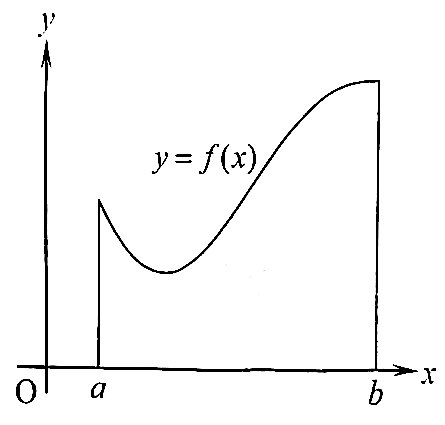
\includegraphics[scale=0.3]{assets/28-3.jpg}
\end{center}

Shown in the diagram above (shaded area) is the area bounded by the line $x =
    a$, $x = b$, $y = 0$, and the curve $y = f(x)$ where $f(x) \geq 0$. This kind
of graph is called the curved trapezoid.

\begin{center}
    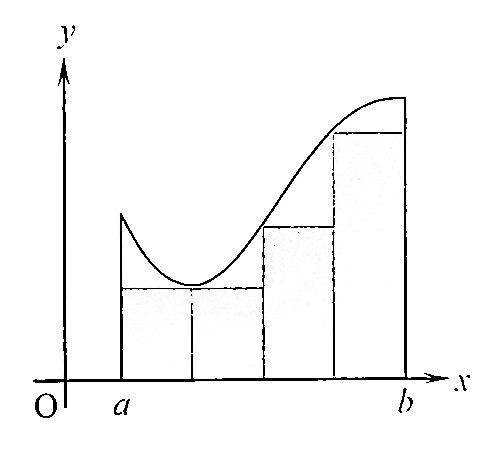
\includegraphics[scale=0.3]{assets/28-1.jpg}
    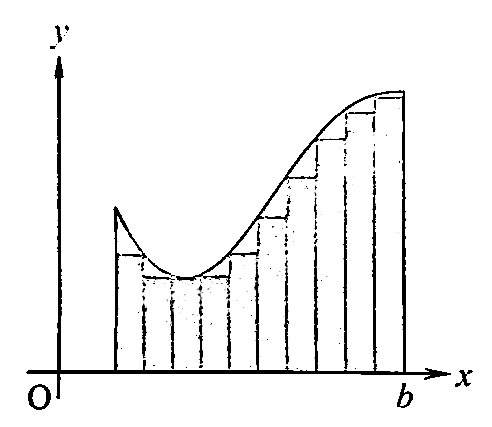
\includegraphics[scale=0.3]{assets/28-2.jpg}
    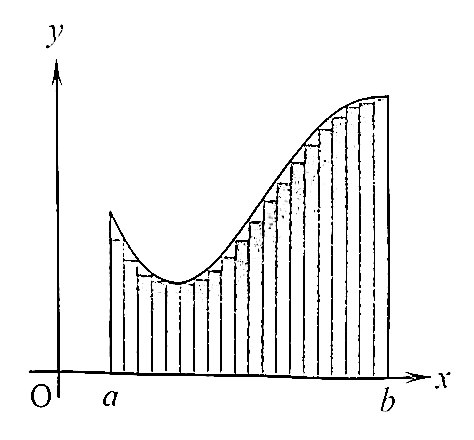
\includegraphics[scale=0.3]{assets/28-4.jpg}
\end{center}

As shown in the diagram above, in order to find the area of this curved
trapezoid, we can split it into multiple small curved trapezoid, each of them
being substituted by their respective rectangular shape. As such, an
approximate value of the area of the curved trapezoid can be acquired by
summing up of the area of each rectangle. As the curved trapezoid is being
split into smaller and smaller pieces, the approximate value we get will get
closer and closer to its actual area.

With this concept in mind, we can split the interval $[a, b]$ into $n$ smaller
interval $[x_0, x_1]$, $[x_1, x_2]$, $\cdots$, $[x_{n-1}, x_n]$ where $x_0 =
    a$, $x_n = b$. From drawing lines that are perpendicular to the $x$-axis
through the points $x_1$, $x_2$, $\cdots$, $x_{n-1}$, we can split the curved
trapezoid into $n$ smaller curved trapezoid.

\begin{center}
    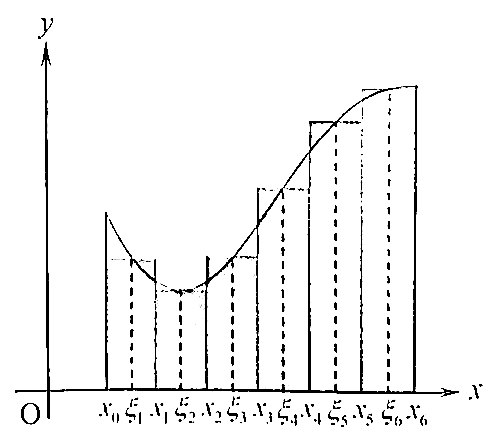
\includegraphics[scale=0.3]{assets/28-5.jpg}
\end{center}

Choose any point $\xi_i$ in the $i$-th interval $[x_{i-1}, x_i]$, then the area
$\Delta A$ of the $i$-th curved trapezoid can be approximated by the area of
the rectangle with width $\Delta x_i = x_i - x_{i-1}$ and height $f(\xi_i)$, as
shown in the diagram above, i.e.
\begin{cequation}
    \Delta A_i \approx f(\xi_i)\Delta x
\end{cequation}
And the approximated value of the area of the original curved trapezoid is the sum of the area of all the smaller rectangle, i.e.
\begin{cequation}
    A = \sum_{i=1}^n \Delta A_i \approx \sum_{i=1}^n f(\xi_i)\Delta x
\end{cequation}

As the number of smaller interval $n$ increases and the width of each interval
decreases, the approximated value of the area of the original curved trapezoid
gets closer and closer to its actual area. To find the value of $A$, we split
the interval $[a, b]$ into indefinitely many smaller interval such that $\Delta
    x \to 0$ (i.e. $n \to \infty$), hence the area of the original curved trapezoid
can be defined as the limit of the sum of the area of all the smaller
rectangle, i.e.
\begin{cequation}
    A = \lim_{n \to \infty} \sum_{i=1}^n f(\xi_i)\Delta x
\end{cequation}

This limit is called the definite integral of $f(x)$ from $a$ to $b$, and is
denoted by the symbol $\displaystyle\int_a^b f(x) dx$, i.e.
\begin{cequation}
    \int_a^b f(x) dx = \lim_{n \to \infty} \sum_{i=1}^n f(\xi_i)\Delta x
\end{cequation}
where $f(x)$ is called the integrand, $[a, b]$ is called the interval of integration, $a$ and $b$ are called the lower and upper limits of integration respectively.

If $f(x) \geq 0$ in the interval $[a, b]$, we know from the above discussion
that the value of the definite integral $\displaystyle\int_a^b f(x) dx$ is the
area of the curved trapezoid bounded by the curve $y = f(x)$, the $x$-axis, and
the lines $x = a$ and $x = b$, i.e. $A = \displaystyle\int_a^b f(x) dx$.

\vspace{0.5cm}
\begin{vwcol}[widths={0.7,0.3},justify=flush,rule=0pt,indent=1em]
    If $f(x) \leq 0$ in the interval $[a, b]$, as shown in the diagram on the right-hand-side,
    $f(\xi_i)\Delta x$ is the negative value of the area of the $i$-th smaller
    rectangle. Hence, the definite integral $\displaystyle\int_a^b f(x) dx$ is
    negative, and its absolute value is the area of the curved trapezoid bounded by
    the curve $y = f(x)$, the $x$-axis, and the lines $x = a$ and $x = b$, i.e. $A
        = -\displaystyle\int_a^b f(x) dx$.

    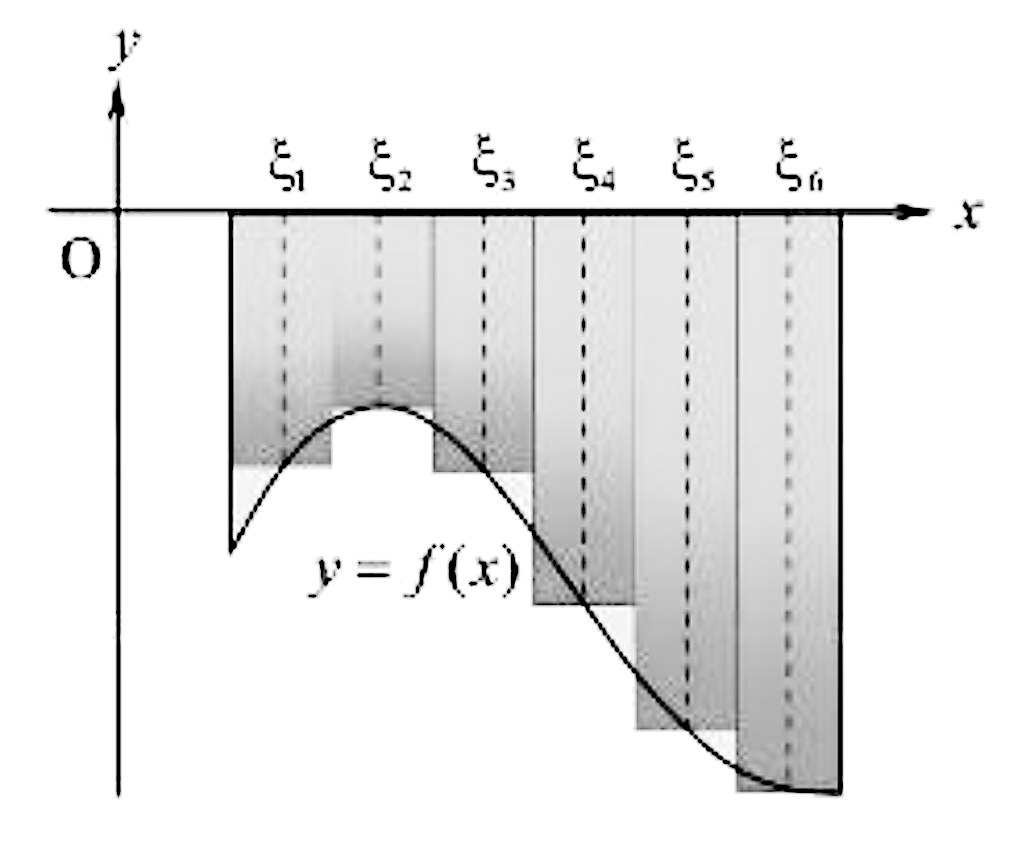
\includegraphics[scale=0.15]{assets/28-4.png}
\end{vwcol}

\newpage

\subsection*{The Relationship between Definite Integrals and Indefinite Integrals}

The definite integrals and the indefinite integrals has inseparable
relationship between them. Consider the case of finding the area of curved
trapezoid. Let $x_0 > a$ and $f(x) \geq 0$. The area of the curved trapezoid
bounded by the curve $y = f(x)$, the $x$-axis, and the lines $x = a$, $x = x_0$
and $y = 0$ is $A(x_0) = \displaystyle\int_a^{x_0} f(x) dx$.

\vspace{0.5cm}
\begin{vwcol}[widths={0.6,0.4},justify=flush,rule=0pt,indent=1em]
    When $x_0$ changes, the area $A(x_0)$ also changes. From the diagram above, we
    know that
    \begin{cequation}
        m\Delta x \leq A(x_0 + \Delta x) - A(x_0) \leq M\Delta x,
    \end{cequation}
    where $m$ and $M$ are the minimum and maximum values of $f(x)$ in the interval $[x_0, x_0 + \Delta x]$. Hence,
    \begin{cequation}
        m \leq \dfrac{A(x_0 + \Delta x) - A(x_0)}{\Delta x} \leq M.
    \end{cequation}

    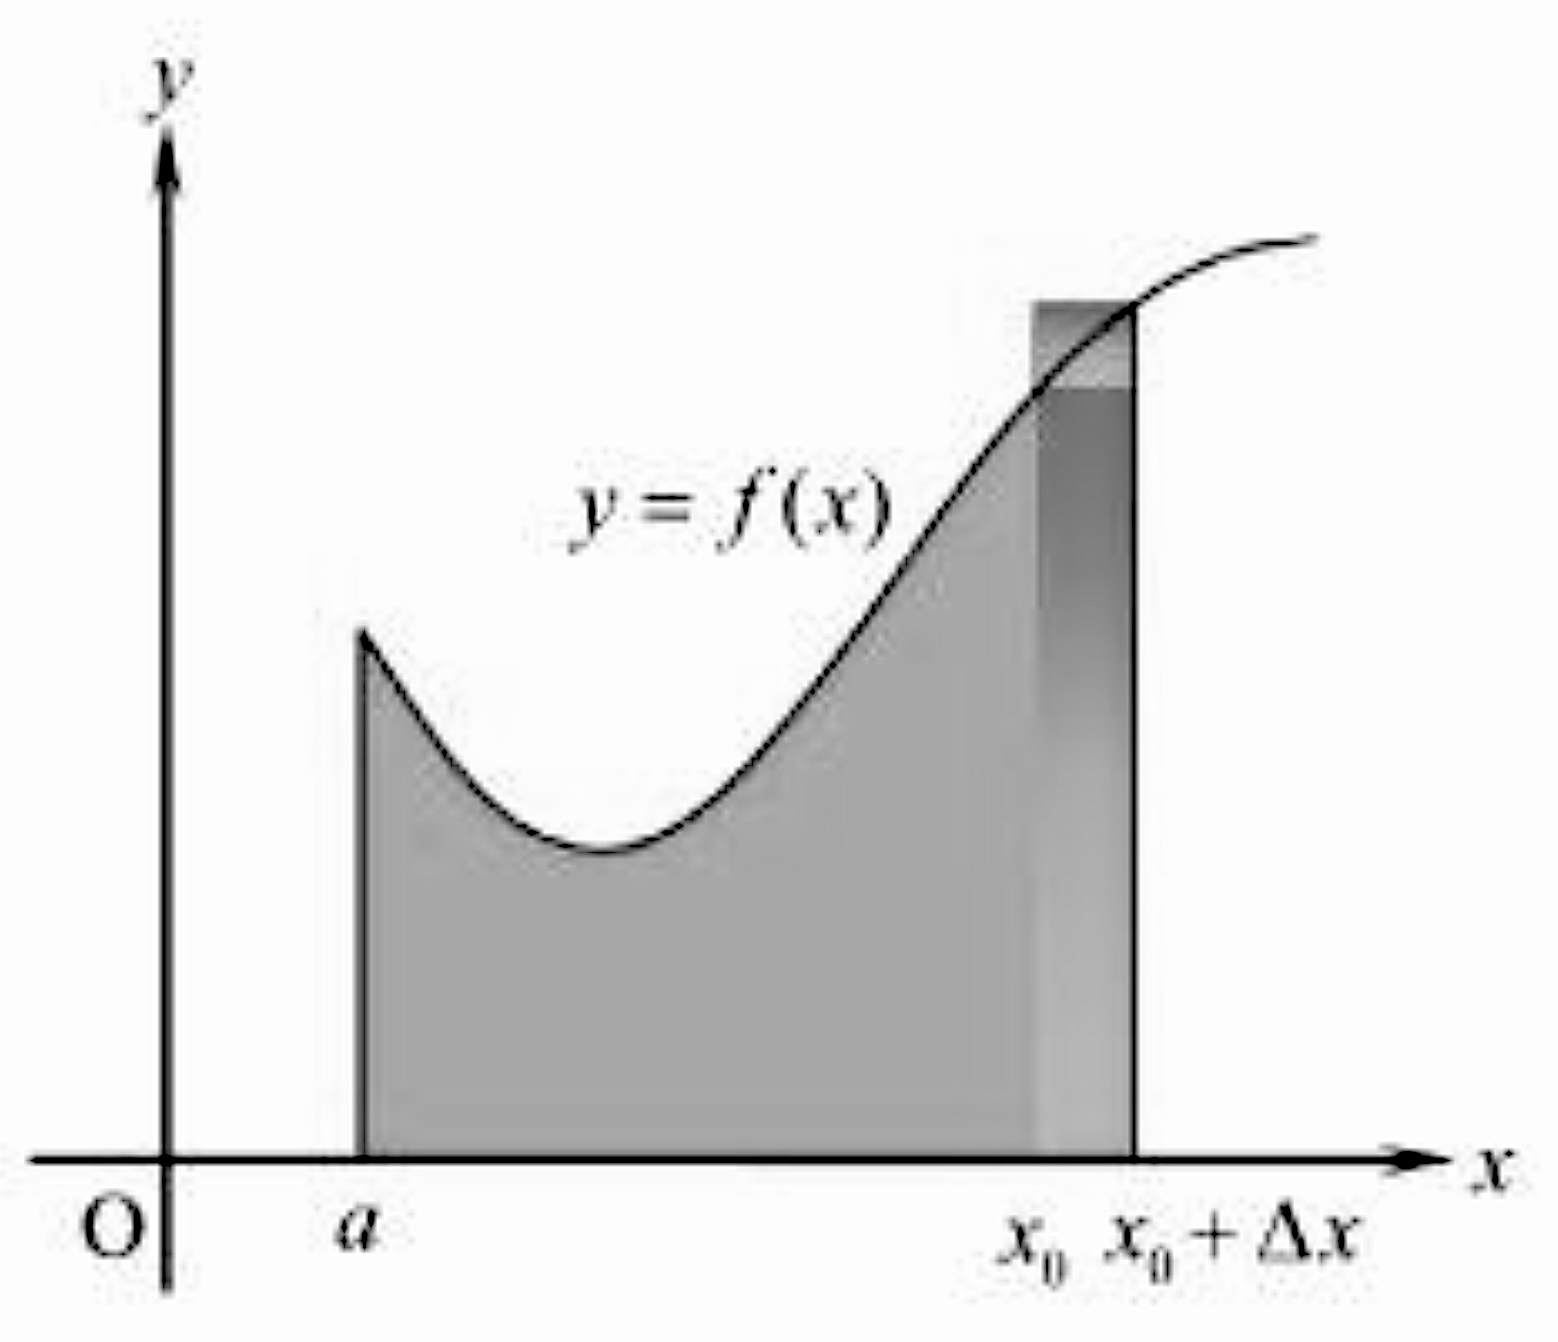
\includegraphics[scale=0.1]{assets/28-7.png}
\end{vwcol}
\vspace{0.5cm}

Apparently, as $\Delta x$ approaches 0, both $m$ and $M$ approach $f(x_0)$.
Besides, from the definition of derivative, \\$\lim_{\Delta x \to 0}
\dfrac{A(x_0 + \Delta x) - A(x_0)}{\Delta x} = A'(x_0)$. Hence, we get $A'(x_0)
= f(x_0)$. This relational expression is true for any $x_0 > a$. In other
    words, $A'(x) = f(x)$, i.e. the derivative of the area function $A(x)$ is the
    integrand $f(x)$.

    Let $\displaystyle\int f(x)d x = F(x) + C$, i.e. $F(x)$ is the primitive of
$f(x)$. Then, from $A'(x) = f(x) = F'(x)$, we get $A(x) = F(x) + C$, where $C$
    is a constant. When $A(a) = 0$, $x = a$, we get $C = -F(a)$. Hence, $C =
-F(a)$, i.e. for any $x_0 > a$, we get $A(x_0) = F(x_0) - F(a)$.

    Let $x_0 = b$, we get $A(b) = \displaystyle\int_a^b f(x) dx = F(b) - F(a)$.
    This relational expression is true for any continuous function $f(x)$. In order
    to make the relational expression true for any $a$ and $b$, when $a > b$, the
    following definition is made.
    \begin{center}
        \framebox{

            \parbox[t][1.3cm]{6cm}{ \addvspace{0.2cm} \centering $\displaystyle\int_a^b f(x) dx
                    = -\int_b^a f(x) dx$ }}
    \end{center}

    Above all are the relationship between definite integrals and indefinite
    integrals, i.e. \vspace{-0.9em}
    \begin{center}
        \framebox{

            \parbox[t][1.3cm]{9cm}{ \addvspace{0.2cm} \centering If $\displaystyle\int f(x) dx
                    = F(x) + C$, then $\displaystyle\int_a^b f(x) dx = F(b) - F(a)$. }}
    \end{center}
    This relationship is called the fundamental theorem of calculus. Generally, we
    express the expression as follows:
    \begin{cequation}
        \int_a^b f(x) dx = \big[F(x)\big]_a^b = F(b) - F(a).
    \end{cequation}
    where $F(x)$ is any primitive of $f(x)$.

    When finding the definite integral $\displaystyle\int_a^b f(x) dx$, we only
    have to find any primitive $F(x)$ of $f(x)$. The other primitive of $f(x)$ can
    be expressed as $F(x) + C$, where $C$ is a constant. Hence, the definite
    integral $\displaystyle\int_a^b f(x) dx$ is independent of the choice of
    primitive of $f(x)$. But,
    \begin{flalign*}
         & \big[F(x) + C\big]_a^b = [F(b) + C] - [F(a) + C] = F(b) - F(a)
    \end{flalign*}
    Hence, the value of the definite integral has nothing to do with the constant $C$. The value of the definite integral remains the same no matter which primitive of $f(x)$ is chosen.

    Note that $\big[F(x)\big]_a^b$ can also be written as $F(x)\big|_a^b$.

    \newpage
    \subsection{Practice 2}

\begin{enumerate}
    \begin{multicols}{2}
        \item $\displaystyle\int_2^8 x d x$
        \sol{}
        \begin{flalign*}
            I & = \left[\dfrac{1}{2}x^2\right]_2^8 & \\
              & = \dfrac{1}{2}(64 - 4)             & \\
              & = 30
        \end{flalign*}

        \item $\displaystyle\int_{-2}^4 x^3 d x$
        \sol{}
        \begin{flalign*}
            I & = \left[\dfrac{1}{4}x^4\right]_{-2}^4 & \\
              & = \dfrac{1}{4}(256 - 16)              & \\
              & = 60
        \end{flalign*}
    \end{multicols}
    \begin{multicols}{2}
        \item $\displaystyle\int_{-\pi}^\pi \cos x d x$
        \sol{}
        \begin{flalign*}
            I & = \bigg[\sin x\bigg]_{-\pi}^\pi & \\
              & = \sin\pi - \sin(-\pi)          & \\
              & = 0 - 0                         & \\
              & = 0
        \end{flalign*}

        \item $\displaystyle\int_0^{\frac{\pi}{4}} \sec ^2 x d x$
        \sol{}
        \begin{flalign*}
            I & = \bigg[\tan x\bigg]_0^{\frac{\pi}{4}} & \\
              & = \tan\dfrac{\pi}{4} - \tan 0          & \\
              & = 1 - 0                                & \\
              & = 1
        \end{flalign*}
    \end{multicols}
\end{enumerate}
    \subsection{Exercise 28.1}

\begin{enumerate}
    \begin{multicols}{2}
        \item $\displaystyle\int_{-2}^4 x^2 d x$
        \sol{}
        \begin{flalign*}
            I & = \left[\dfrac{1}{3}x^3\right]_{-2}^4 & \\
              & = \dfrac{1}{3}(64 + 8)                & \\
              & = 24
        \end{flalign*}
        \item $\displaystyle\int_1^4 \dfrac{1}{x^2} d x$
        \sol{}
        \begin{flalign*}
            I & = \left[-\dfrac{1}{x}\right]_1^4 & \\
              & = -\dfrac{1}{4} + 1              & \\
              & = \dfrac{3}{4}
        \end{flalign*}
    \end{multicols}

    \begin{multicols}{2}
        \item $\displaystyle\int_4^9 \sqrt{x} d x$
        \sol{}
        \begin{flalign*}
            I & = \left[\dfrac{2}{3}x^{\frac{3}{2}}\right]_4^9 & \\
              & = \dfrac{2}{3}(27 - 8)                         & \\
              & = \dfrac{38}{3}
        \end{flalign*}

        \item $\displaystyle\int_1^{27} \dfrac{1}{\sqrt[3]{x^5}} d x$
        \sol{}
        \begin{flalign*}
            I & = \left[-\dfrac{3}{2}x^{-\frac{2}{3}}\right]_1^{27} & \\
              & = -\dfrac{3}{2}\left(\dfrac{1}{9} - 1\right)        & \\
              & = \dfrac{4}{3}
        \end{flalign*}
    \end{multicols}
    \newpage
    \begin{multicols}{2}
        \item $\displaystyle\int_0^{\frac{\pi}{3}} \cos x d x$
        \sol{}
        \begin{flalign*}
            I & = \bigg[\sin x\bigg]_0^{\frac{\pi}{3}} & \\
              & = \sin\dfrac{\pi}{3} - \sin 0          & \\
              & = \dfrac{\sqrt{3}}{2} - 0              & \\
              & = \dfrac{\sqrt{3}}{2}
        \end{flalign*}

        \item $\displaystyle\int_{-\frac{\pi}{4}}^{\frac{\pi}{2}} \sin x d x$
        \sol{}
        \begin{flalign*}
            I & = \bigg[-\cos x\bigg]_{-\frac{\pi}{4}}^{\frac{\pi}{2}} & \\
              & = -\cos\dfrac{\pi}{2} - (-\cos(-\frac{\pi}{4}))        & \\
              & = 0 + \dfrac{\sqrt{2}}{2}                              & \\
              & = \dfrac{\sqrt{2}}{2}
        \end{flalign*}
    \end{multicols}

    \begin{multicols}{2}
        \item $\displaystyle\int_0^2 e^x d x$
        \sol{}
        \begin{flalign*}
            I & = e^2 - e^0 & \\
              & = e^2 - 1
        \end{flalign*}
        \vfill{}\null{}
        \columnbreak{}
        \item $\displaystyle\int_{\frac{\pi}{4}}^{\frac{\pi}{2}} \operatorname{cosec}^2 x d x$
        \sol{}
        \begin{flalign*}
            I & = \bigg[-\cot x\bigg]_{\frac{\pi}{4}}^{\frac{\pi}{2}} & \\
              & = -\cot\frac{\pi}{2} + \cot\frac{\pi}{4}              & \\
              & = 0 + 1                                               & \\
              & = 1
        \end{flalign*}
    \end{multicols}

    \begin{multicols}{2}
        \item $\displaystyle\int_1^2 \dfrac{1}{x} d x$
        \sol{}
        \begin{flalign*}
            I & = = \bigg[\ln|x|\bigg]_1^2 & \\
              & = \ln 2 - \ln 1            & \\
              & = \ln 2
        \end{flalign*}

        \item $\displaystyle\int_0^2 \dfrac{1}{x+1} d x$
        \sol{}
        \begin{flalign*}
            I & = \bigg[\ln|x+1|\bigg]_0^2 & \\
              & = \ln 3 - \ln 1            & \\
              & = \ln 3                    & \\
        \end{flalign*}
    \end{multicols}
\end{enumerate}

\newpage


    \section{Properties and Calculations of Definite Integrals}

    \subsection*{Properties of Definite Integrals}

    \noindent \hspace{1.2em}\textit{The definite integrals have the following basic properties:}

    \begin{center}
        \framebox{

            \parbox[t][1.3cm]{10cm}{ \addvspace{0.2cm}\hspace{10pt}\textbf{Property 1}
                \hspace{10pt} $\displaystyle\int_a^b kf(x) dx = k\int_a^b f(x) dx$}}
    \end{center}
    \begin{center}
        \framebox{

        \parbox[t][1.3cm]{10cm}{ \addvspace{0.2cm}\hspace{10pt} \textbf{Property 2}
        \hspace{10pt} $\displaystyle\int_a^b [f(x) \pm g(x)] dx = \int_a^b f(x) dx \pm
            \int_a^b g(x) dx$}}
    \end{center}
    \begin{center}
        \framebox{

            \parbox[t][1.3cm]{10cm}{ \addvspace{0.25cm}\hspace{10pt}\textbf{Property 3}
                \hspace{10pt} $\displaystyle\int_c^a f(x) dx + \int_b^c f(x) dx = \int_b^a f(x)
                    dx$}}
    \end{center}

    \subsection{Practice 3}

\noindent \hspace{1.2em}\textit{
    Find the extreme values of the following functions (Question 1 to 4):
}

\begin{enumerate}
    \item $f(x)=x^2+x-6$
    \item $f(x)=2-x-x^2$
    \item $f(x)=\dfrac{1}{3} x^3-\dfrac{1}{2} x^2-2x+2$
    \item $f(x)=4 x-3 x^3$
\end{enumerate}

\noindent \hspace{1.2em}\textit{Find the coordinates of the extreme points of the following functions (Question 5 to 6):}
\begin{enumerate}[resume]
    \item $y=2 x^3-3 x^2-12 x-7$
    \item $y=x+\dfrac{1}{x}$
\end{enumerate}



    \subsection*{Integration by Substitution}

    In the last chapter, we have learned how to solve indefinite integrals using
    the method of integration by substitution: $\displaystyle\int f(g(x))g'(x)dx =
\int f(u)du$ where $u = g(x)$. From the basic theorem of calculus, the method
    of integration by substitution of definite integrals can be derived:
    \begin{center}
        \framebox{

            \parbox[t][1.3cm]{9cm}{ \addvspace{0.2cm} \centering $\displaystyle\int_a^b
                    f(g(x))g'(x)dx = \int_{g(a)}^{g(b)} f(u)du$ }}
    \end{center}
    \vspace{0.9em}
    The method of integration by substitution of definite integrals is similar to
    that of indefinite integrals. The only difference is that the limits of
    integration are changed accordingly.

    \subsection{Practice 4}

\noindent \hspace{1.2em}\textit{Find the absolute maximum value and the absolute minimum value of the following functions (Question 1 to 2):}
\begin{enumerate}
    \item $f(x) = 3x^3 - 9x + 5$, $[-2, 2]$
    \item $f(x) = x^4 - 2x^2 + 5$, $[-2, 3]$
    \item If $x + y = 8$, find the absolute minimum value of $x^2 + y^2$.
    \item A metal wire with a length of $100$cm is bent into a rectangle. Find the width
          and the length of the rectangle so that the area of the rectangle is the
          largest.
\end{enumerate}

    \newpage

    \subsection{Exercise 28.2}

\begin{enumerate}
    \begin{multicols}{2}
        \item $\displaystyle\int_0^4\left(x^2-2 x\right) d x$
        \sol{}
        \begin{flalign*}
            I & = \bigg[\dfrac{1}{3}x^3 - x^2\bigg]_0^4 & \\
              & = \dfrac{64}{3} - 16                    & \\
              & = \dfrac{16}{3}
        \end{flalign*}
        \item $\displaystyle\int_1^4 \dfrac{2 x^2-3 \sqrt{x}+1}{x} d x$
        \sol{}
        \begin{flalign*}
            I & = \int_1^4 \left(2x - 3x^{-\frac{1}{2}} + x^{-1}\right) d x & \\
              & = \bigg[x^2 - 6\sqrt{x} + \ln|x|\bigg]_1^4                  & \\
              & = 16 - 12 + \ln 4 - 1 + 6 - \ln 1                           & \\
              & = 9 + \ln 4
        \end{flalign*}
    \end{multicols}

    \begin{multicols}{2}
        \item $\displaystyle\int_{-3}^3(x+3)^2 d x$
        \sol{}

        Let $u = x + 3$, $du = dx$.

        When $x = -3$, $u = 0$.

        When $x = 3$, $u = 6$.
        \begin{flalign*}
            I & = \int_0^6 u^2 d u                & \\
              & = \bigg[\dfrac{1}{3}u^3\bigg]_0^6 & \\
              & = 72
        \end{flalign*}

        \item $\displaystyle\int_{-1}^1(2+x)\left(2-x^2\right) d x$
        \sol{}
        \begin{flalign*}
            I & = \int_{-1}^1\left(4 - 2x^2 + 2x - x^3\right)dx                             & \\
              & = \bigg[4x - \dfrac{2}{3}x^3 + x^2 - \dfrac{1}{4}x^4\bigg]_{-1}^1           & \\
              & = 4 - \dfrac{2}{3} + 1 - \dfrac{1}{4} + 4 - \dfrac{2}{3} - 1 + \dfrac{1}{4} & \\
              & = \dfrac{20}{3}
        \end{flalign*}
    \end{multicols}

    \begin{multicols}{2}
        \item $\displaystyle\int_0^{\frac{\pi}{2}}(2 \sin 3 \theta-3 \cos 2 \theta) d \theta$
        \sol{}
        \begin{flalign*}
            I & = \bigg[-\dfrac{2}{3}\cos 3\theta - \dfrac{3}{2}\sin 2\theta\bigg]_0^{\frac{\pi}{2}} & \\
              & = \dfrac{2}{3} + \dfrac{3}{2} + \dfrac{2}{3}                                         & \\
              & = \dfrac{13}{6}
        \end{flalign*}
        \vfill{}\null{}
        \columnbreak{}

        \item $\displaystyle\int_0^{\frac{\pi}{3}} \tan \theta d \theta$
        \sol{}
        \begin{flalign*}
            I & = \int_0^{\frac{\pi}{3}} \dfrac{\sin \theta}{\cos \theta} d \theta &
        \end{flalign*}
        Let $u = \cos \theta$, $du = -\sin \theta d \theta$.

        When $\theta = 0$, $u = 1$.

        When $\theta = \dfrac{\pi}{3}$, $u = \dfrac{1}{2}$.
        \begin{flalign*}
            I & = -\int_1^{\frac{1}{2}} \dfrac{1}{u} d u & \\
              & = -\bigg[\ln|u|\bigg]_1^{\frac{1}{2}}    & \\
              & = -\ln\dfrac{1}{2} + \ln 1               & \\
              & = \ln 2
        \end{flalign*}
    \end{multicols}

    \newpage

    \begin{multicols}{2}
        \item $\displaystyle\int_0^1\left(e^x-1\right)^2 d x$
        \sol{}
        \begin{flalign*}
            I & = \int_0^1\left(e^{2x} - 2e^x + 1\right) d x    & \\
              & = \bigg[\dfrac{1}{2}e^{2x} - 2e^x + x\bigg]_0^1 & \\
              & = \dfrac{1}{2}e^2 - 2e + 1 - \dfrac{1}{2} + 2   & \\
              & = \dfrac{1}{2}e^2 - 2e + \dfrac{5}{2}           & \\
              & = \dfrac{e^2 - 4e + 5}{2}
        \end{flalign*}
        \vfill{}\null{}

        \item $\displaystyle\int_1^4 \dfrac{2}{4 x-1} d x$
        \sol{}

        Let $u = 4x - 1$, $du = 4dx$.

        When $x = 1$, $u = 3$.

        When $x = 4$, $u = 15$.
        \begin{flalign*}
            I & = \dfrac{1}{2}\int_3^{15} \dfrac{1}{u} d u & \\
              & = \dfrac{1}{2}\bigg[\ln|u|\bigg]_3^{15}    & \\
              & = \dfrac{1}{2}(\ln 15 - \ln 3)             & \\
              & = \dfrac{1}{2}\ln 5
        \end{flalign*}
    \end{multicols}

    \begin{multicols}{2}
        \item $\displaystyle\int_{-1}^3 \sqrt{2 x+3} d x$
        \sol{}

        Let $u = 2x + 3$, $du = 2dx$.

        When $x = -1$, $u = 1$.

        When $x = 3$, $u = 9$.
        \begin{flalign*}
            I & = \dfrac{1}{2}\int_1^9 \sqrt{u} d u           & \\
              & = \dfrac{1}{3}\bigg[u^{\frac{3}{2}}\bigg]_1^9 & \\
              & = \dfrac{1}{3}(27 - 1)                        & \\
              & = \dfrac{26}{3}
        \end{flalign*}

        \item $\displaystyle\int_1^2 \dfrac{1}{(2 x-1)^3} d x$
        \sol{}

        Let $u = 2x - 1$, $du = 2dx$.

        When $x = 1$, $u = 1$.

        When $x = 2$, $u = 3$.
        \begin{flalign*}
            I & = \dfrac{1}{2}\int_1^3 u^{-3} d u                & \\
              & = -\dfrac{1}{4}\bigg[u^{-2}\bigg]_1^3            & \\
              & = -\dfrac{1}{4}\left(\dfrac{1}{9} - 1\right)     & \\
              & = -\dfrac{1}{4} \cdot \left(-\dfrac{8}{9}\right) & \\
              & = \dfrac{2}{9}
        \end{flalign*}
    \end{multicols}

    \begin{multicols}{2}
        \item $\displaystyle\int_{-1}^1 x^2\left(x^3-1\right)^4 d x$
        \sol{}

        Let $u = x^3 - 1$, $du = 3x^2dx$.

        When $x = -1$, $u = -2$.

        When $x = 1$, $u = 0$.
        \begin{flalign*}
            I & = \dfrac{1}{3}\int_{-2}^0 u^4 d u     & \\
              & = \dfrac{1}{15}\bigg[u^5\bigg]_{-2}^0 & \\
              & = \dfrac{32}{15}
        \end{flalign*}
        \columnbreak{}

        \item $\displaystyle\int_1^6 x \sqrt{3 x-2} d x$
        \sol{}

        Let $u = 3x - 2$, $du = 3dx$, $x = \dfrac{u + 2}{3}$.

        When $x = 1$, $u = 1$.

        When $x = 6$, $u = 16$.
        \begin{flalign*}
            I & = \dfrac{1}{3}\int_1^{16} \dfrac{u + 2}{3}\sqrt{u} d u                                     & \\
              & = \dfrac{1}{9}\int_1^{16} \left(u^{\frac{3}{2}} + 2u^{\frac{1}{2}}\right) d u              & \\
              & = \dfrac{1}{9}\bigg[\dfrac{2}{5}u^{\frac{5}{2}} + \dfrac{4}{3}u^{\frac{3}{2}}\bigg]_1^{16} & \\
              & = \dfrac{1}{9}\left(\dfrac{2048}{5} + \dfrac{256}{3} - \dfrac{2}{5} - \dfrac{4}{3}\right)  & \\
              & = \dfrac{274}{5}
        \end{flalign*}
    \end{multicols}

    \newpage
    \item $\displaystyle\int_{-\frac{\pi}{4}}^{\frac{\pi}{4}} \sin ^2 \theta d \theta$
          \sol{}
          \begin{flalign*}
              I & = \dfrac{1}{2}\int_{-\frac{\pi}{4}}^{\frac{\pi}{4}} (1 - \cos 2\theta) d \theta              & \\
                & = \dfrac{1}{2}\bigg[\theta - \dfrac{1}{2}\sin 2\theta\bigg]_{-\frac{\pi}{4}}^{\frac{\pi}{4}} & \\
                & = \dfrac{1}{2}\left(\dfrac{\pi}{4} - \dfrac{1}{2} + \dfrac{\pi}{4} - \dfrac{1}{2}\right)     & \\
                & = \dfrac{\pi}{4} - \dfrac{1}{2}                                                              & \\
                & = \dfrac{\pi - 2}{4}
          \end{flalign*}

    \item $\displaystyle\int_3^5 \dfrac{1}{x^2-x-2} d x$
          \sol{}
          \begin{flalign*}
              I & = \int_3^5 \dfrac{1}{(x-2)(x+1)} d x &
          \end{flalign*}
          Let $\dfrac{1}{(x-2)(x+1)} = \dfrac{A}{x-2} + \dfrac{B}{x+1}$.
          \begin{flalign*}
              Ax + A + Bx - 2B    & = 1 \\
              (A + B)x + (A - 2B) & = 1
          \end{flalign*}
          \vspace{-2em}
          \begin{flalign*}
              \begin{cases}
                  A + B = 0 \\
                  A - 2B = 1
              \end{cases}
              \Rightarrow
              \begin{cases}
                  A = \dfrac{1}{3} \\
                  B = -\dfrac{1}{3}
              \end{cases}
          \end{flalign*}
          \vspace{-1em}
          \begin{flalign*}
              I & = \int_3^5 \left(\dfrac{1}{3(x-2)} - \dfrac{1}{3(x+1)}\right) d x       & \\
                & = \dfrac{1}{3}\int_3^5 \left(\dfrac{1}{x-2} - \dfrac{1}{x+1}\right) d x & \\
                & = \dfrac{1}{3}\bigg[\ln|x-2| - \ln|x+1|\bigg]_3^5                       & \\
                & = \dfrac{1}{3}\left(\ln 3 - \ln 6 - \ln 1 + \ln 4\right)                & \\
                & = \dfrac{1}{3}\ln 2
          \end{flalign*}

          \newpage

          \begin{multicols}{2}
              \item $\displaystyle\int_2^5 \dfrac{x}{x^3-x^2-x+1} d x$
              \sol{}
              \begin{flalign*}
                  I & = \int_2^5 \dfrac{x}{x^2(x-1) - (x-1)} d x & \\
                    & = \int_2^5 \dfrac{x}{(x^2 - 1)(x-1)} d x   & \\
                    & = \int_2^5 \dfrac{x}{(x + 1)(x-1)^2} d x
              \end{flalign*}
              Let $\dfrac{x}{(x + 1)(x-1)^2} = \dfrac{A}{x+1} + \dfrac{B}{x-1} + \dfrac{C}{(x-1)^2}$.
              \begin{flalign*}
                  Ax^2 - 2Ax + A + Bx^2 - B + Cx + C    & = x & \\
                  (A + B)x^2 + (-2A + C)x + (A - B + C) & = x
              \end{flalign*}
              \vspace{-2em}
              \begin{flalign*}
                  \begin{cases}
                      A + B = 0   \\
                      -2A + C = 1 \\
                      A - B + C = 0
                  \end{cases}
                  \Rightarrow
                  \begin{cases}
                      A = -\dfrac{1}{4} \\
                      B = \dfrac{1}{4}  \\
                      C = \dfrac{1}{2}
                  \end{cases}
              \end{flalign*}
              \vspace{-1em}
              \begin{flalign*}
                  I & = \int_2^5 \left(-\dfrac{1}{4(x+1)} + \dfrac{1}{4(x-1)} + \dfrac{1}{2(x-1)^2}\right) d x                       & \\
                    & = \left[-\dfrac{1}{4}\ln|x+1| + \dfrac{1}{4}\ln|x-1| - \dfrac{1}{2(x-1)}\right]_2^5                            & \\
                    & = -\dfrac{1}{4}\ln 6 + \dfrac{1}{4}\ln 4 - \dfrac{1}{8} + \dfrac{1}{4}\ln 3 - \dfrac{1}{4}\ln 1 + \dfrac{1}{2} & \\
                    & = -\dfrac{1}{4}\ln 6 + \dfrac{1}{4}\ln 4 - \dfrac{1}{8} + \dfrac{1}{4}\ln 3 + \dfrac{1}{2}                     & \\
                    & = \dfrac{1}{4}\ln 2 + \dfrac{3}{8}
              \end{flalign*}

              \item $\displaystyle\int_0^1 \dfrac{x^2}{x^2+2 x+1} d x$
              \sol{}
              \begin{flalign*}
                  I & = \int_0^1 \dfrac{x^2}{(x+1)^2} d x &
              \end{flalign*}
              Let $u = x + 1$, $du = dx$, $x = u - 1$.

              When $x = 0$, $u = 1$.

              When $x = 1$, $u = 2$.
              \begin{flalign*}
                  I & = \int_1^2 \dfrac{(u - 1)^2}{u^2} d u                         & \\
                    & = \int_1^2 \dfrac{u^2 - 2u + 1}{u^2} d u                      & \\
                    & = \int_1^2 \left(1 - \dfrac{2}{u} + \dfrac{1}{u^2}\right) d u & \\
                    & = \bigg[u - 2\ln|u| - \dfrac{1}{u}\bigg]_1^2                  & \\
                    & = 2 - 2\ln 2 - \dfrac{1}{2} - 1 + 2\ln 1 + 1                  & \\
                    & = \dfrac{3}{2} - 2\ln 2
              \end{flalign*}
          \end{multicols}

          \begin{multicols}{2}
              \item $\displaystyle\int_0^3 \dfrac{x}{\sqrt{25-x^2}} d x$
              \sol{}

              Let $u = 25 - x^2$, $du = -2xdx$.

              When $x = 0$, $u = 25$.

              When $x = 3$, $u = 16$.
              \begin{flalign*}
                  I & = \dfrac{1}{2}\int_{16}^{25} \dfrac{1}{\sqrt{u}} d u & \\
                    & = \bigg[\sqrt{u}\bigg]_{16}^{25}                     & \\
                    & = 5 - 4                                              & \\
                    & = 1
              \end{flalign*}

              \item $\displaystyle\int_0^{\frac{\pi}{6}} \sin ^2 \theta \cos \theta d \theta$
              \sol{}

              Let $u = \sin \theta$, $du = \cos \theta d \theta$.

              When $\theta = 0$, $u = 0$.

              When $\theta = \dfrac{\pi}{6}$, $u = \dfrac{1}{2}$.
              \begin{flalign*}
                  I & = \int_0^{\frac{1}{2}} u^2 d u                & \\
                    & = \bigg[\dfrac{1}{3}u^3\bigg]_0^{\frac{1}{2}} & \\
                    & = \dfrac{1}{24}
              \end{flalign*}
          \end{multicols}

          \newpage
    \item Given that $f(x)=\left\{\begin{array}{cc}2 x^2-1, & -2 \leq x \leq 2 \\ 3 x+1, & 2<x \leq 4\end{array}\right.$, find $\displaystyle\int_{-2}^4 f(x) d x$.
          \sol{}
          \begin{flalign*}
              I & = \int_{-2}^2 (2x^2 - 1) d x + \int_2^4 (3x + 1) d x                           & \\
                & = \bigg[\dfrac{2}{3}x^3 - x\bigg]_{-2}^2 + \bigg[\dfrac{3}{2}x^2 + x\bigg]_2^4 & \\
                & = \dfrac{16}{3} - 2 + \dfrac{16}{3} - 2 + 24 + 4 - 6 - 2                       & \\
                & = \dfrac{80}{3}
          \end{flalign*}

    \item Given that $\displaystyle\int_3^5 f(x) d x=6, \int_5^9 f(x) d x=18, \int_1^4
              g(x) d x=4$ and $\displaystyle\int_3^4 g(x) d x=-4$. Find:
          \begin{enumerate}
              \item $\displaystyle\int_1^3 g(x) d x$;
                    \sol{}
                    \begin{flalign*}
                        \int_1^3 g(x) d x & = \int_1^4 g(x) d x - \int_3^4 g(x) d x & \\
                                          & = 4 - (-4)                              & \\
                                          & = 8
                    \end{flalign*}

              \item $\displaystyle\int_1^3 f(3 x) d x$;
                    \sol{}

                    Let $u = 3x$, $du = 3dx$.

                    When $x = 1$, $u = 3$.

                    When $x = 3$, $u = 9$.
                    \begin{flalign*}
                        \int_1^3 f(3 x) d x & = \dfrac{1}{3}\int_3^9 f(u) d u                                 & \\
                                            & = \dfrac{1}{3}\int_3^5 f(u) d u + \dfrac{1}{3}\int_5^9 f(u) d u & \\
                                            & = \dfrac{1}{3}(6 + 18)                                          & \\
                                            & = 8
                    \end{flalign*}

              \item $\displaystyle\int_1^3[f(3 x)-3 g(x)] d x$.
                    \sol{}
                    \begin{flalign*}
                        \int_1^3[f(3 x)-3 g(x)] d x & = \int_1^3 f(3 x) d x - 3\int_1^3 g(x) d x & \\
                                                    & = 8 - 3 \cdot 8                            & \\
                                                    & = -16
                    \end{flalign*}
          \end{enumerate}
          \newpage

          \begin{multicols}{2}
              \item Given the function $y=x \sqrt{x+1}$, \\find $\dfrac{d y}{d x}$. Hence, find
              $\displaystyle\int_3^8 \dfrac{3 x+2}{\sqrt{x+1}} d x$. \sol{}
              \begin{flalign*}
                  \dfrac{d y}{d x}                       & = \sqrt{x + 1} + \dfrac{x}{2\sqrt{x + 1}}  & \\
                                                         & = \dfrac{2x + x + 2}{2\sqrt{x + 1}}        & \\
                                                         & = \dfrac{3x + 2}{2\sqrt{x + 1}}            & \\
                  \\
                  \int_3^8 \dfrac{3 x+2}{\sqrt{x+1}} d x & = 2\int_3^8 \dfrac{3 x+2}{2\sqrt{x+1}} d x & \\
                                                         & = 2\int_3^8 \dfrac{d y}{d x} d x           & \\
                                                         & = 2\left[x \sqrt{x + 1}\right]_3^8         & \\
                                                         & = 2\left(24 - 6\right)                     & \\
                                                         & = 36
              \end{flalign*}
              \vfill{}\null{}

              \item Given the function $y=\dfrac{x^2-1}{2 x+1}$, \\find $\dfrac{d y}{d x}$. Hence,
              find $\displaystyle\int_0^2 \dfrac{x^2+x+1}{4 x^2+4 x+1} d x$. \sol{}
              \begin{flalign*}
                  \dfrac{d y}{d x}                          & = \dfrac{(2x + 1)(2x) - (x^2 - 1)(2)}{(2x + 1)^2}             & \\
                                                            & = \dfrac{4x^2 + 2x - 2x^2 + 2}{(2x + 1)^2}                    & \\
                                                            & = \dfrac{2(x^2 + x + 1)}{(2x + 1)^2}                          & \\
                  \\
                  \int_0^2 \dfrac{x^2+x+1}{4 x^2+4 x+1} d x & = \dfrac{1}{2}\int_0^2 \dfrac{2(x^2 + x + 1)}{(2x + 1)^2} d x & \\
                                                            & = \dfrac{1}{2}\int_0^2 \dfrac{d y}{d x} d x                   & \\
                                                            & = \dfrac{1}{2}\left[\dfrac{x^2 - 1}{2x + 1}\right]_0^2        & \\
                                                            & = \dfrac{1}{2}\left(\dfrac{3}{5} - \dfrac{-1}{1}\right)       & \\
                                                            & = \dfrac{4}{5}
              \end{flalign*}
              \vfill\null{}
          \end{multicols}

    \item Given the function $y=x e^x-e^x$, find $\dfrac{d y}{d x}$. Hence, find
          $\displaystyle\int_1^4 2 x e^x d x$. \sol{}
          \begin{flalign*}
              \dfrac{d y}{d x}     & = x e^x + e^x - e^x                & \\
                                   & = x e^x                            & \\
              \\
              \int_1^4 2 x e^x d x & = 2\int_1^4 x e^x d x              & \\
                                   & = 2\int_1^4 \dfrac{d y}{d x} d x   & \\
                                   & = 2\left[x e^x - e^x\right]_1^4    & \\
                                   & = 2\left(4e^4 - e^4 - e + e\right) & \\
                                   & = 6e^4
          \end{flalign*}
\end{enumerate}

\newpage


    \section{Area}

    When we first introduced the concept of definite integrals, we have studied
    that, if $f(x) \geq 0$ in the interval $a \leq x \leq b$, then the area of the
    curved trapezoid bounded by the curve $y = f(x)$, the lines $x = a$ and $x =
b$, the $x$-axis, and the $y$-axis is given by
    \begin{cequation}
        A = \int_a^b f(x)dx
    \end{cequation}

    The applications of definite integrals are not limited to finding area of
    curved trapezoid. In fact, it is widely used in different fields of
    technologies. To solve real-life problems, the basic mindset is the steps
    described in the definition: splitting, approximating, finding sum, and taking
    limit. After understanding the concept, part of the steps can be skipped, and
    the related definite integrals can be written out straight away.

    Let's take finding the area of the curved trapezoid bounded by the line $x =
a$, $x = b$, the $x$-axis, and the curve $y = f(x)$ as an example and do some
    further elaboration. Since both sides of the curved trapezoid are the straight
    lines $x = a$ and $x = b$, we can split the interval $a \leq x \leq b$ into
    multiple smaller intervals, hence the original curved trapezoid is split into
    multiple smaller curved trapezoid. As shown in the diagram below, take any one
    of the smaller intervals, and express it as $[x, x + \Delta x]$, its
    corresponding smaller curved trapezoid can be approximated by a rectangle with
    width of $\Delta x$ and height of the function value $f(x)$ at the point $x$.
    As such, the area of the smaller curved trapezoid is $\Delta A \approx
f(x)\Delta x$.
    \begin{center}
        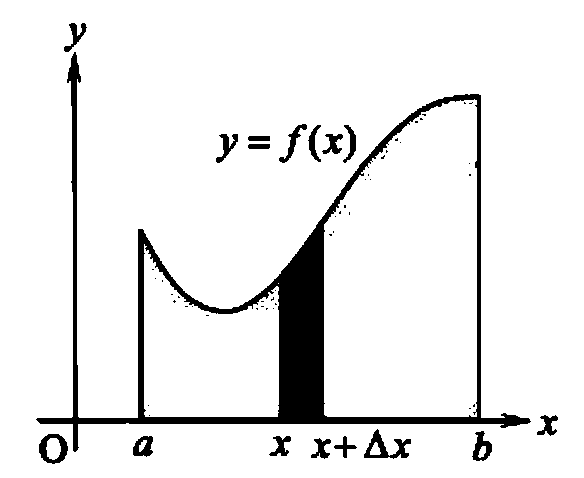
\includegraphics[scale=0.3]{assets/28-8.png}
    \end{center}

    Summing up the approximated area of all the smaller curved trapezoid, then find
    the limit of the sum when $\Delta x \to 0$, we can get the area of the original
    curved trapezoid, i.e.
    \begin{cequation}
        \sum\Delta A \approx \sum f(x)\Delta x\ \xrightarrow{\ \ \ \ \Delta x \to 0\ \ \ \ } \int_a^b f(x)dx
    \end{cequation}

    \begin{center}
        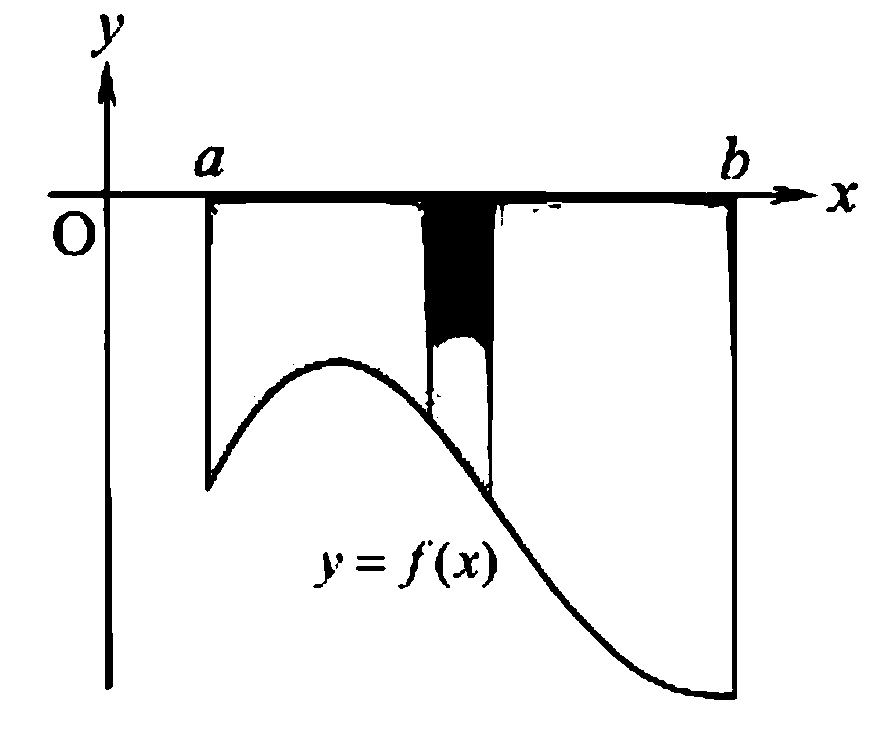
\includegraphics[scale=0.2]{assets/28-9.png}
    \end{center}
    The same can be applied if $f(x) \leq 0$ in the interval $a \leq x \leq b$, as
    shown in the diagram above. The area of the curved trapezoid bounded by the
    curve $y = f(x)$, the lines $x = a$ and $x = b$, the $x$-axis, and the $y$-axis
    is given by
    \begin{cequation}
        A = -\int_a^b f(x)dx
    \end{cequation}

    \begin{center}
        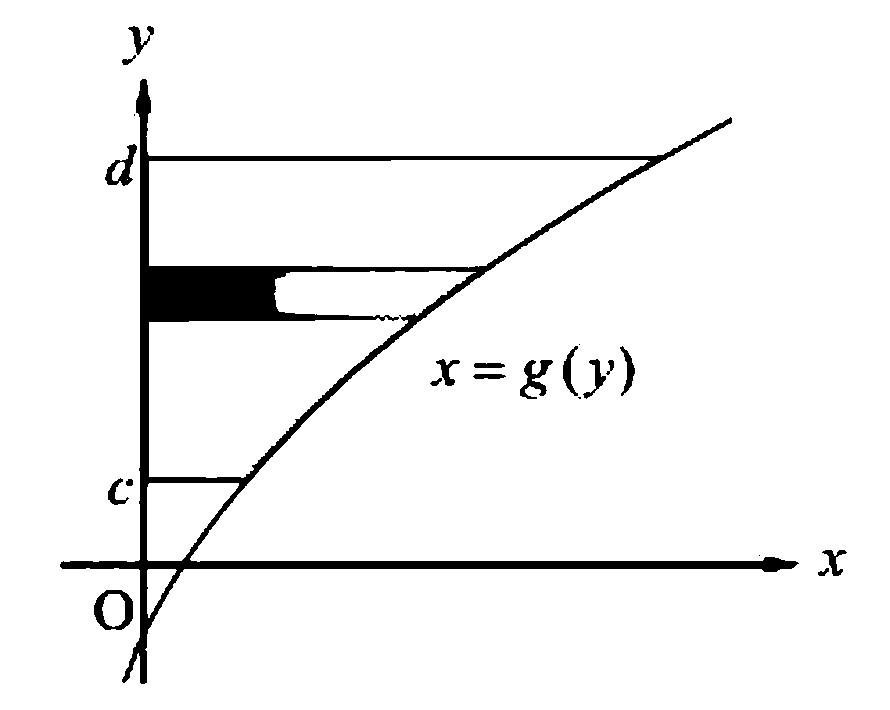
\includegraphics[scale=0.2]{assets/28-10.png}
    \end{center}
    If the target area $A$ is bounded by the lines $y = c$, $y = d$, the $y$-axis,
    and the curve $x = f(y)$, where $f(y) \geq 0$ in the interval $c \leq y \leq
d$, as shown in the diagram above, using the same concept, we can get the area
    of the region
    \begin{cequation}
        A = \int_c^d f(y)dy
    \end{cequation}

    \subsection{Practice 5}
Find the following indefinite integral:
\begin{enumerate}
    \begin{multicols}{2}
        \item $\displaystyle\int\sin2x\cos2x dx$
        \sol{}
        \begin{flalign*}
            I & = \dfrac{1}{2}\int\sin4x dx & \\
              & = -\dfrac{1}{8}\cos4x + C
        \end{flalign*}
        \vfill{}\null{}

        \item $\displaystyle\int\cos^2 2x dx$
        \sol{}
        \begin{flalign*}
            I & = \int\dfrac{1 + \cos 4x}{2} dx                    & \\
              & = \dfrac{1}{2}\int dx + \dfrac{1}{2}\int\cos 4x dx & \\
              & = \dfrac{1}{2}x + \dfrac{1}{8}\sin 4x + C
        \end{flalign*}
    \end{multicols}
    \begin{multicols}{2}
        \item $\displaystyle\int\sin^3 x dx$
        \sol{}
        \begin{flalign*}
            I & = \int\sin^2 x\sin x dx                 & \\
              & = \int(1 - \cos^2 x)\sin x dx           & \\
              & = \int\sin x dx - \int\cos^2 x\sin x dx
        \end{flalign*}
        Let $u = \cos x$, $du = -\sin xdx$.
        \begin{flalign*}
            I & = -\int \cos x dx + \int u^2 du    & \\
              & = -\sin x + \dfrac{1}{3}u^3 + C    & \\
              & = \dfrac{1}{3}\cos^3 x -\sin x + C
        \end{flalign*}

        \item $\displaystyle\int\cos^3 x dx$
        \sol{}
        \begin{flalign*}
            I & = \int\cos^2 x\cos x dx                 & \\
              & = \int(1 - \sin^2 x)\cos x dx           & \\
              & = \int\cos x dx - \int\sin^2 x\cos x dx
        \end{flalign*}
        Let $u = \sin x$, $du = \cos xdx$.
        \begin{flalign*}
            I & = \int \cos x dx - \int u^2 du      & \\
              & = \sin x - \dfrac{1}{3}u^3 + C      & \\
              & = \sin x - \dfrac{1}{3}\sin^3 x + C
        \end{flalign*}
    \end{multicols}
    \begin{multicols}{2}
        \item $\displaystyle\int\tan^4 x\sec^2 x dx$
        \sol{}

        Let $u = \tan x$, $du = \sec^2 xdx$.
        \begin{flalign*}
            I & = \int u^4 du              & \\
              & = \dfrac{u^5}{5} + C       & \\
              & = \dfrac{1}{5}\tan^5 x + C
        \end{flalign*}
        \vfill{}\null{}
        \columnbreak
        \item $\displaystyle\int\tan^4\dfrac{x}{2} dx$
        \sol{}
        \begin{flalign*}
            I & = \int\tan^2\dfrac{x}{2}\tan^2\dfrac{x}{2} dx                             & \\
              & = \int\left(\sec^2\dfrac{x}{2} - 1\right)\tan^2\dfrac{x}{2} dx            & \\
              & = \int\sec^2\dfrac{x}{2}\tan^2\dfrac{x}{2} dx - \int\tan^2\dfrac{x}{2} dx
        \end{flalign*}
        Let $u = \tan\dfrac{x}{2}$, $du = \dfrac{1}{2}\sec^2\dfrac{x}{2}dx$.
        \begin{flalign*}
            I & = 2\int u^2 du - \int \tan^2\dfrac{x}{2} dx                     & \\
              & = \dfrac{2u^3}{3} - \int \left(\sec^2\dfrac{x}{2} - 1\right) dx & \\
              & = \dfrac{2u^3}{3} - \int \sec^2\dfrac{x}{2} dx + \int dx        & \\
              & = \dfrac{2}{3}\tan^3\dfrac{x}{2} - 2\tan\dfrac{x}{2} + x + C
        \end{flalign*}
    \end{multicols}
\end{enumerate}

    \newpage
    If, in the internal $a \leq x \leq b$, $f_2(x) \geq f_1(x) \geq 0$, then the
    area of the region bounded by the curve $y = f_1(x)$, $y = f_2(x)$, the lines
$x = a$ and $x = b$ can be found using definite integrals.
    \begin{center}
        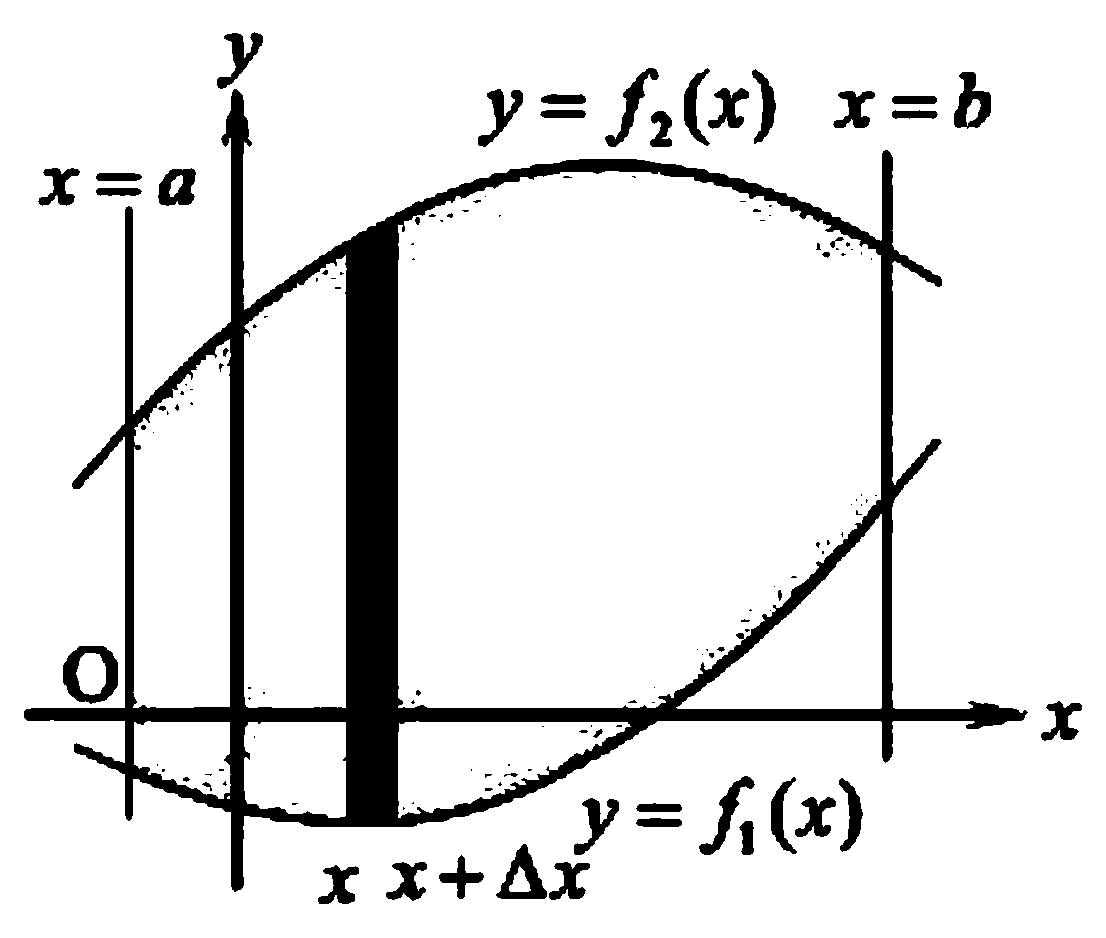
\includegraphics[scale=0.15]{assets/28-16.png}
    \end{center}

    As shown in the diagram above, split the interval $a \leq x \leq b$ into
    multiple smaller intervals. Take any one of the smaller intervals, and express
    it as $[x, x + \Delta x]$. The region in this smaller interval can be
    approximated by a rectangle with width of $\Delta x$ and height of the function
    value $f_2(x) - f_1(x)$, i.e.
    \begin{cequation}
        \Delta A \approx [f_2(x) - f_1(x)]\Delta x
    \end{cequation}

    Summing up the approximated area of all the smaller intervals, then find the
    limit of the sum when $\Delta x \to 0$, we can get the area of the region
    bounded by the curve $y = f_1(x)$, $y = f_2(x)$, the lines $x = a$ and $x = b$,
    i.e.
    \begin{center}
        \framebox{

        \parbox[t][1.3cm]{5cm}{ \addvspace{0.2cm} \centering $\displaystyle A = \int_a^b
            [f_2(x) - f_1(x)]dx$ }}
    \end{center}

    \begin{center}
        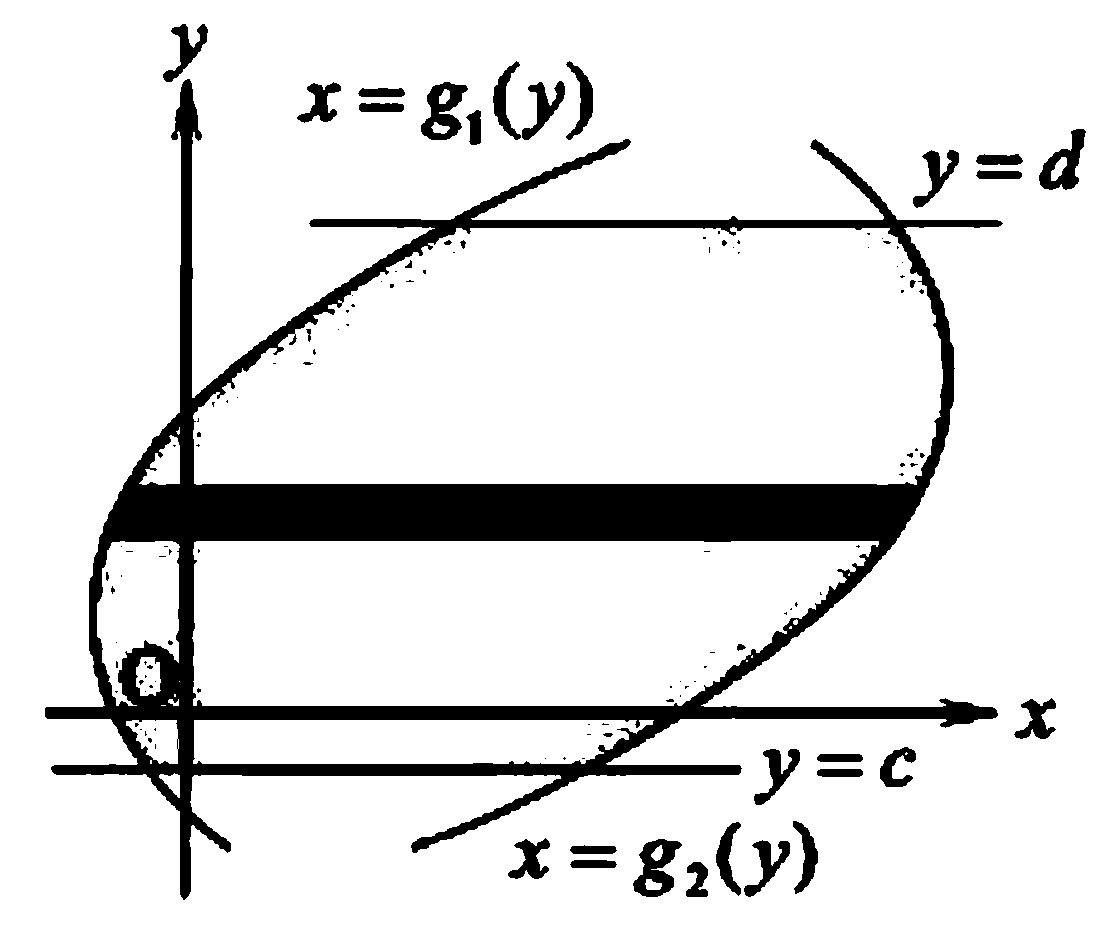
\includegraphics[scale=0.15]{assets/28-17.png}
    \end{center}

    Similarly, if, in the internal $c \leq y \leq d$, $g_2(y) \geq g_1(y) \geq 0$,
    then the area of the region bounded by the curve $x = g_1(y)$, $x = g_2(y)$,
    the lines $y = c$ and $y = d$ is given by
    \begin{center}
        \framebox{

        \parbox[t][1.3cm]{5cm}{ \addvspace{0.2cm} \centering $\displaystyle A = \int_c^d
            [g_2(y) - g_1(y)]dy$ }}
    \end{center}
    Note that when using these formulas, the function $f_2(x)$ must always be greater than or equal to $f_1(x)$ in the interval $[a, b]$.

    \newpage
    \subsection{Practice 6}

Sketch the graph of the function $f(x) = x^3 - 3x^2 + 2$.

    \subsection{Exercise 28.3}

\noindent \hspace{1.2em}\textit{Find the area of the region bounded by the following curves and lines:}
\begin{enumerate}
      \begin{multicols}{2}
            \item $y=3 x^2, x=2, x=5$, and $x$-axis
            \sol{}
            \begin{flalign*}
                  A & = \int_2^5 3x^2 d x    & \\
                    & = \left[x^3\right]_2^5 & \\
                    & = 125 - 8              & \\
                    & = 117
            \end{flalign*}

            \item $y=(x-1)^2, x=4, x$-axis, and $y$-axis
            \sol{}
            \begin{flalign*}
                  A & = \int_0^4 (x-1)^2 d x                 & \\
                    & = \left[\dfrac{1}{3}(x-1)^3\right]_0^4 & \\
                    & = \dfrac{1}{3}(3^3 + 1)                & \\
                    & = \dfrac{28}{3}
            \end{flalign*}
      \end{multicols}

      \vfill\null

      \begin{multicols}{2}
            \item $y=x^2+4 x-21$, and $x$-axis
            \begin{flalign*}
                  x^2 + 4x - 21        & = 0 & \\
                  (x + 7)(x - 3)       & = 0 & \\
                  x = -7 \text{ or } x & = 3
            \end{flalign*}
            In the interval $-7 \leq x \leq 3$, $x^2 + 4x - 21 \leq 0$.
            \begin{flalign*}
                  A & = \left|\int_{-7}^3 (x^2 + 4x - 21) d x\right|                       & \\
                    & = \left|\left[\dfrac{1}{3}x^3 + 2x^2 - 21x\right]_{-7}^3\right|      & \\
                    & = \left|9 + 18 - 63 - \left(-\dfrac{343}{3} + 98 + 147\right)\right| & \\
                    & = \dfrac{500}{3}
            \end{flalign*}

            \item $y=e^{2 x}, x=0, x=4$, and $x$-axis
            \sol{}
            \begin{flalign*}
                  A & = \int_0^4 e^{2x} d x                 & \\
                    & = \left[\dfrac{1}{2}e^{2x}\right]_0^4 & \\
                    & = \dfrac{1}{2}(e^8 - 1)
            \end{flalign*}
      \end{multicols}

      \vfill\null

      \begin{multicols}{2}
            \item $y=\sin \dfrac{x}{2}, 0 \leq x \leq 2 \pi$, and $x$-axis
            \sol{}
            \begin{flalign*}
                  A & = \int_0^{2 \pi} \sin \dfrac{x}{2} d x        & \\
                    & = \left[-2 \cos \dfrac{x}{2}\right]_0^{2 \pi} & \\
                    & = 4
            \end{flalign*}
            \vfill\null

            \columnbreak
            \item $y=\cos x, x=2 \pi, x$-axis, and $y$-axis
            \sol{}
            \begin{flalign*}
                  \cos x & = 0                                & \\
                  x      & = \dfrac{\pi}{2}, \dfrac{3 \pi}{2}
            \end{flalign*}
            In the interval $\dfrac{\pi}{2} \leq x \leq \dfrac{3 \pi}{2}$, $\cos x \leq 0$.
            \begin{flalign*}
                  A & = \int_{0}^{\frac{\pi}{2}} \cos x d x + \left|\int_{\frac{\pi}{2}}^{\frac{3 \pi}{2}} \cos x d x\right| + \int_{\frac{3 \pi}{2}}^{2 \pi} \cos x d x        & \\
                    & = \bigg[\sin x\bigg]_0^{\frac{\pi}{2}} + \left|\bigg[\sin x\bigg]_{\frac{\pi}{2}}^{\frac{3 \pi}{2}}\right| + \bigg[\sin x\bigg]_{\frac{3 \pi}{2}}^{2 \pi} & \\
                    & = 1 + 1 + 1 + 1 = 4
            \end{flalign*}
      \end{multicols}

      \newpage
      \begin{multicols}{2}
            \item $x=y^2, y=3$, and $y$-axis
            \sol{}
            \begin{flalign*}
                  A & = \int_0^3 y^2 d y                 & \\
                    & = \left[\dfrac{1}{3}y^3\right]_0^3 & \\
                    & = 9
            \end{flalign*}

            \vfill{}\null{}
            \columnbreak{}
            \item $x=9 y-y^3$, and $y$-axis
            \sol{}
            \begin{flalign*}
                  9y - y^3   & = 0                   & \\
                  y(9 - y^2) & = 0                   & \\
                  y = 0      & \text{ or } y = \pm 3
            \end{flalign*}
            In the interval $-3 \leq y \leq 0$, $9y - y^3 \leq 0$.
            \begin{flalign*}
                  A & = \left|\int_{-3}^0 (9y - y^3) d y\right| + \int_0^3 (9y - y^3) d y                                                       & \\
                    & = \left|\left[\dfrac{9}{2}y^2 - \dfrac{1}{4}y^4\right]_{-3}^0\right| + \left[\dfrac{9}{2}y^2 - \dfrac{1}{4}y^4\right]_0^3 & \\
                    & = \left|- \dfrac{81}{2} + \dfrac{81}{4}\right| + \dfrac{81}{2} - \dfrac{81}{4}                                            & \\
                    & = \dfrac{81}{2}
            \end{flalign*}
      \end{multicols}

      \begin{multicols}{2}
            \item $y=\dfrac{1}{x}, y=\dfrac{1}{2}, y=2$, and $y$-axis
            \sol{}
            \begin{flalign*}
                  A & = \int_{\frac{1}{2}}^2 \dfrac{1}{x} d x & \\
                    & = \bigg[\ln x\bigg]_{\frac{1}{2}}^2     & \\
                    & = \ln 2 - \ln \dfrac{1}{2}              & \\
                    & = 2 \ln 2
            \end{flalign*}

            \item $y^2=x, x=4$, and $x=16$
            \sol{}
            \begin{flalign*}
                  A & = 2 \int_4^{16} \sqrt{x} d x                        & \\
                    & = 2 \left[\dfrac{2}{3}x^{\frac{3}{2}}\right]_4^{16} & \\
                    & = 2 \left(\dfrac{128}{3} - \dfrac{16}{3}\right)     & \\
                    & = \dfrac{224}{3}
            \end{flalign*}
            \vfill{}\null{}
      \end{multicols}

      \begin{multicols}{2}
            \item Find the area of the region bounded by the curve \\$y=x^2-4$ and the line $y=3
            x$. \sol{}
                  \begin{flalign*}
                        x^2 - 4             & = 3x & \\
                        x^2 - 3x - 4        & = 0  & \\
                        (x - 4)(x + 1)      & = 0  & \\
                        x = 4 \text{ or } x & = -1
                  \end{flalign*}
                  In the interval $-1 \leq x \leq 4$, $x^2 - 4 \leq 3x$.
                  \begin{flalign*}
                        A & = \int_{-1}^4 (3x - x^2 + 4) d x                             & \\
                          & = \left[\dfrac{3}{2}x^2 - \dfrac{1}{3}x^3 + 4x\right]_{-1}^4 & \\
                          & = 24 - \dfrac{64}{3} + 16 - \dfrac{3}{2} - \dfrac{1}{3} + 4  & \\
                          & = \dfrac{125}{6}
                  \end{flalign*}
                  \item Find the area of the region bounded by the curve $y=x^2+2 x$ and the curve
            $y=12+4 x-x^2$.
                  \begin{flalign*}
                        x^2 + 2x            & = 12 + 4x - x^2 & \\
                        2x^2 - 2x - 12      & = 0             & \\
                        (x - 3)(2x + 4)     & = 0             & \\
                        x = 3 \text{ or } x & = -2
                  \end{flalign*}
                  In the interval $-2 \leq x \leq 3$, $x^2 + 2x \leq 12 + 4x - x^2$.
            \begin{flalign*}
                  A & = \int_{-2}^3 (12 + 4x - x^2 - x^2 - 2x) d x      & \\
                    & = \int_{-2}^3 (12 + 2x - 2x^2) d x                & \\
                    & = \left[12x + x^2 - \dfrac{2}{3}x^3\right]_{-2}^3 & \\
                    & = 36 + 9 - 18 + 24 - 4 - \dfrac{16}{3}            & \\
                    & = \dfrac{125}{3}
            \end{flalign*}
      \end{multicols}

      \begin{multicols}{2}
            \item Find the area of the region bounded by the curve $y=\sin x$ and $y=-2 \sin x$
            in the interval $0 \leq x \leq \pi$. \sol{}
            \begin{flalign*}
                  \sin x & = -2 \sin x & \\
                  \sin x & = 0         & \\
                  x      & = 0, \pi
            \end{flalign*}
            In the interval $0 \leq x \leq \pi$, $-2 \sin x \leq \sin x$.
            \begin{flalign*}
                  A & = \int_0^{\pi} (3 \sin x) d x   & \\
                    & = \bigg[-3 \cos x\bigg]_0^{\pi} & \\
                    & = 3 - (-3) = 6
            \end{flalign*}
            \vfill{}\null{}

            \item Find the area of the region bounded by the curve $y=e^x, y=e^{-2 x}$ and the
            lines $x=-2$ and $x=4$. \sol{}
            \begin{flalign*}
                  e^x & = e^{-2x} & \\
                  x   & = 0
            \end{flalign*}
            In the interval $-2 \leq x \leq 0$, $e^x \leq e^{-2x}$.

            In the interval $0 \leq x \leq 4$, $e^{-2x} \leq e^x$.
            \begin{flalign*}
                  A & = \int_{-2}^0 (e^{-2x} - e^x) d x + \int_0^4 (e^x - e^{-2x}) d x                               & \\
                    & = \left[-\dfrac{1}{2}e^{-2x} - e^x\right]_{-2}^0 + \left[e^x + \dfrac{1}{2}e^{-2x}\right]_0^4  & \\
                    & = -\dfrac{1}{2} - 1 + \dfrac{1}{2}e^{4} + e^{-2} + e^4 + \dfrac{1}{2}e^{-8} - 1 - \dfrac{1}{2} & \\
                    & = \dfrac{3}{2}e^4 + e^{-2} + \dfrac{1}{2}e^{-8} - 3
            \end{flalign*}
      \end{multicols}

      \vfill\null

      \item Find the area of the region bounded by the curve $y=x^3-10 x^2+28 x$ and the
            line $y=4 x$. \sol{}
            \begin{flalign*}
                  x^3 - 10x^2 + 28x   & = 4x                  & \\
                  x^3 - 10x^2 + 24x   & = 0                   & \\
                  x(x^2 - 10x + 24)   & = 0                   & \\
                  x = 0 \text{ or } x & = 4 \text{ or } x = 6
            \end{flalign*}
            In the interval $0 \leq x \leq 4$, $x^3 - 10x^2 + 28x \geq 4x$.

            In the interval $4 \leq x \leq 6$, $x^3 - 10x^2 + 28x \leq 4x$.
            \begin{flalign*}
                  A & = \int_0^4 (x^3 - 10x^2 + 28x - 4x) d x + \int_4^6 (4x - x^3 + 10x^2 - 28x) d x                                              & \\
                    & = \int_0^4 (x^3 - 10x^2 + 24x) d x + \int_4^6 (-x^3 + 10x^2 - 24x) d x                                                       & \\
                    & = \left[\dfrac{1}{4}x^4 - \dfrac{10}{3}x^3 + 12x^2\right]_0^4 + \left[-\dfrac{1}{4}x^4 + \dfrac{10}{3}x^3 - 12x^2\right]_4^6 & \\
                    & = 64 - \dfrac{640}{3} + 192 - 324 + 720 - 432 + 64 - \dfrac{640}{3} + 192                                                    & \\
                    & = \dfrac{148}{3}
            \end{flalign*}
            \vfill\null

            \newpage

      \item Find the area of the region bounded by the curve $x=8 y-y^2, x=16 y-y^2-48$,
            and $y$-axis. \sol{}
            \begin{flalign*}
                  8y - y^2 & = 16y - y^2 - 48 & \\
                  8y       & = 48             & \\
                  y        & = 6
            \end{flalign*}

      \item Find the area of the region bounded by the curve $x=2 y^2-8 y+10$ and
            $x=y^2-y$.
      \item Given that the curve $y=f(x)$ passes through point $(1,0)$, and the gradient of
            any point on the curve $(x, y)$ is $3 x^2-3$. Find the area of the region
            bounded by the curve, $x=2$ and $x$.
\end{enumerate}

    \newpage
    \section{Volume of Revolution}
    The solid formed by rotating a flat surface around a certain straight line on
    the surface is called the \textbf{solid of revolution}, for example the right
    cylinder, right cone, and sphere.

    \begin{center}
        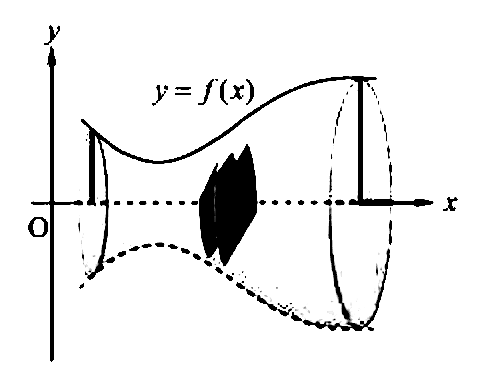
\includegraphics[scale=0.3]{assets/28-22a.png}
    \end{center}

    The diagram above shows a solid of revolution formed by rotating the area
    bounded by the curve $y = f(x)$, the lines $x = a$, $x = b$, and the $x$-axis
    around the $x$-axis. We can utilize the methods discussed in the last section
    to find the volume of this solid of revolution.

    \vspace{0.5cm}
    \begin{vwcol}[widths={0.7,0.3},justify=flush,rule=0pt,indent=1em]

        Split the interval $a \leq x \leq b$ into multiple smaller intervals. Take any
        one of the smaller intervals, and express it as $[x, x + \Delta x]$. The region
        in this smaller interval can be approximated by a rectangle with width of
        $\Delta x$ and height of the function value $f(x)$. Rotate this rectangle
        around the $x$-axis, we get a cylinder with radius $f(x)$ and height $\Delta
            x$, as shown in the diagram on the right-hand side. Hence, the approximated
        volume of the solid of revolution in this smaller interval is
        \begin{cequation}
            \Delta V \approx \pi[f(x)]^2\Delta x
        \end{cequation}

        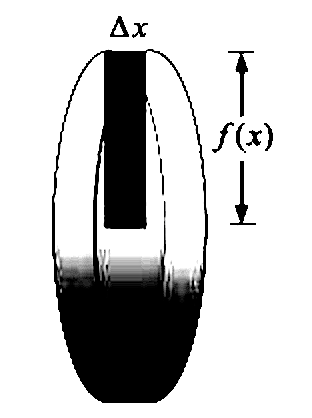
\includegraphics[scale=0.3]{assets/28-22b.png}
    \end{vwcol}
    \vspace{0.5cm}
    Summing up the approximated volume of all the smaller intervals, then find the
    limit of the sum when $\Delta x \to 0$, we can get the volume of the solid of
    revolution, i.e.
    \begin{center}
        \framebox{

        \parbox[t][1.3cm]{4cm}{ \addvspace{0.2cm} \centering $\displaystyle V =
            \pi\int_a^b[f(x)]^2dx$ }}
    \end{center}
    \begin{center}
        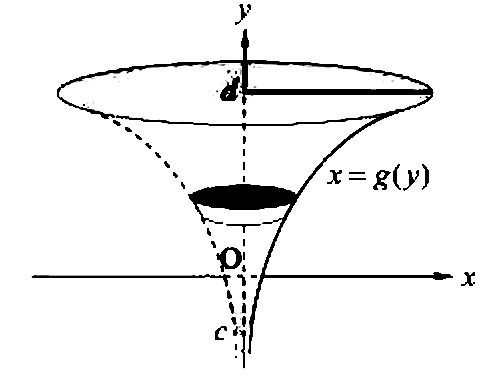
\includegraphics[scale=0.3]{assets/28-23.png}
    \end{center}

    Similarly, if the solid of revolution is formed by rotating the area bounded by
    the curve $x = g(y)$, the lines $y = c$, $y = d$, and the $y$-axis around the
$y$-axis, then the volume of the solid of revolution is given by
    \begin{center}
        \framebox{

        \parbox[t][1.3cm]{4cm}{ \addvspace{0.2cm} \centering $\displaystyle V =
            \pi\int_c^d[g(y)]^2dy$ }}
    \end{center}

    \newpage
    \subsection{Practice 7}
\begin{enumerate}
      \begin{multicols}{2}
            \item A drop of ink gradually spread after being dropped onto a piece of paper. At
            $t$ seconds, its area is $A = \left(3t^2 + \dfrac{1}{5}t + 2\right)$mm$^2$.
            Find the rate of change of the ink spread at $t = 2$ second. \sol{}
            \begin{flalign*}
                  \dfrac{dA}{dt} & = 6t + \dfrac{1}{5}
            \end{flalign*}
            When $t = 2$,
            \begin{flalign*}
                  \dfrac{dA}{dt} & = 6(2) + \dfrac{1}{5}      \\
                                 & = 12 + \dfrac{1}{5}        \\
                                 & = \dfrac{61}{5}            \\
                                 & = 12.2\text{mm}^2\text{/s}
            \end{flalign*}
            \vfill\null

            \item The radius of a sphere increases at a rate of $3$cm/s. When the radius is
            $5$cm, find the rate of change of the surface area of the sphere. \sol{}
            \begin{flalign*}
                  \dfrac{dr}{dt} & = 3\text{cm/s}                      \\
                  A              & = 4\pi r^2                          \\
                  \dfrac{dA}{dr} & = 8\pi r                            \\
                  \dfrac{dA}{dt} & = \dfrac{dA}{dr}\cdot\dfrac{dr}{dt} \\
                                 & = 8\pi r\cdot 3\text{cm/s}          \\
                                 & = 24\pi r\text{cm}^2\text{/s}
            \end{flalign*}
            When $r = 5$,
            \begin{flalign*}
                  \dfrac{dA}{dt} & = 24\pi(5)\text{cm}^2\text{/s} \\
                                 & = 120\pi\text{cm}^2\text{/s}
            \end{flalign*}
      \end{multicols}
\end{enumerate}

    If a region is bounded by the curve $y = f_1(x)$, $y = f_2(x)$, the lines $x =
a$, $x = b$, and the $x$-axis, and $f_2 \geq f_1 \geq 0$, then the volume of
    the solid of revolution formed by rotating this region around the $x$-axis, as
    shown in the diagram below, is given by
    \begin{center}
        \framebox{

        \parbox[t][1.3cm]{12cm}{ \addvspace{0.2cm} \centering $\displaystyle V =
            \pi\int_a^b[f_2(x)]^2dx - \pi\int_a^b[f_1(x)]^2dx =
            \pi\int_a^b\left\{[f_2(x)]^2 - [f_1(x)]^2\right\}dx$ }}
    \end{center}
    \begin{center}
        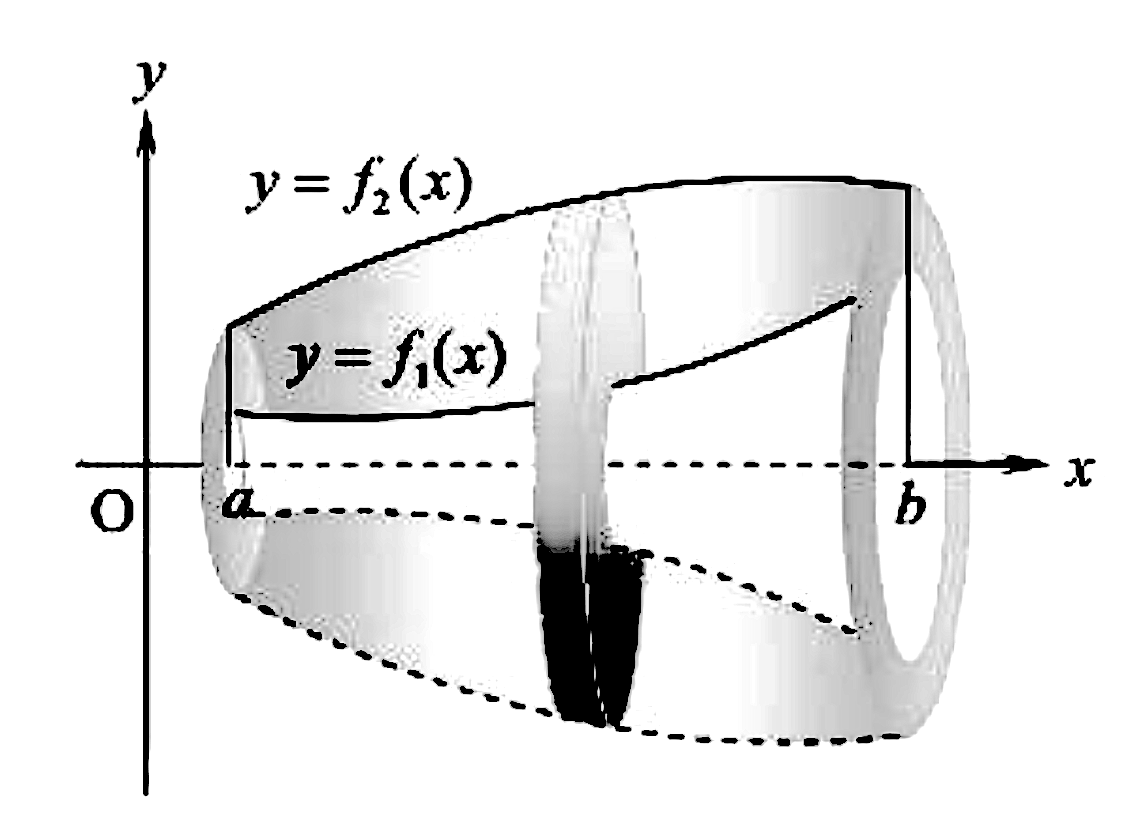
\includegraphics[scale=0.15]{assets/28-29.png}
    \end{center}

    Similarly, if a region is bounded by the curve $x = g_1(y)$, $x = g_2(y)$, the
    lines $y = c$, $y = d$, and the $y$-axis, and $g_2 \geq g_1 \geq 0$, then the
    volume of the solid of revolution formed by rotating this region around the
$y$-axis, as shown in the diagram below, is given by \vspace{-0.9em}
\begin{center}
    \framebox{

    \parbox[t][1.3cm]{6cm}{ \addvspace{0.2cm} \centering $\displaystyle V =
        \pi\int_c^d\left\{[g_2(y)]^2 - [g_1(y)]^2\right\}dy$ }}
\end{center}
\begin{center}
    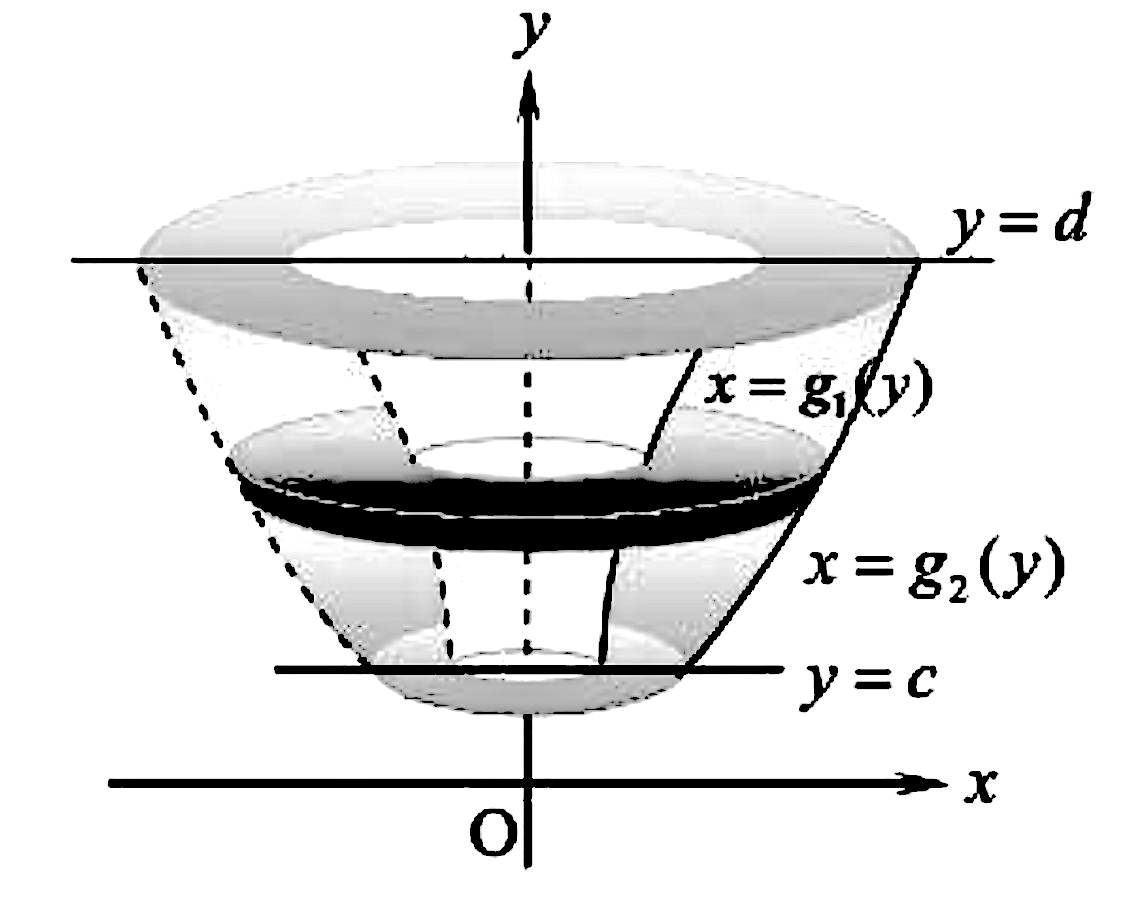
\includegraphics[scale=0.15]{assets/28-30.png}
\end{center}

\subsection{Practice 8}

\begin{enumerate}
      \item The side length of a cube increases from 1cm to $1.01$cm, how much does its
            surface area increase approximately? \sol{}

            Let the side length be $x$cm, then the surface area is $A = 6x^2$.
            \begin{flalign*}
                  \dfrac{dA}{dx}             & = 12x                  & \\
                  \dfrac{\Delta A}{\Delta x} & \approx \dfrac{dA}{dx} & \\
                  \Delta A                   & \approx 12x\Delta x
            \end{flalign*}
            \vspace{-0.8em}
            When $x = 1$cm, $\Delta x = 0.01$cm,
            \begin{flalign*}
                  \Delta A & \approx 12(1)(0.01) = 0.12\text{cm}^2 &
            \end{flalign*}
            $\therefore$ The surface area increases by $0.12$cm$^2$ approximately.

            \begin{multicols}{2}
                  \item After a metal ball was heated, its radius had increased form 4cm to $4.01$cm.
                  Find the approximate increment of its volume and surface area. \sol{}

                  Let the radius be $r$cm, then the volume is $V = \dfrac{4}{3}\pi r^3$ and the
                  surface area is $A = 4\pi r^2$.
                  \begin{flalign*}
                        \dfrac{dV}{dr}             & = 4\pi r^2               & \\
                        \dfrac{dA}{dr}             & = 8\pi r                 & \\
                        \dfrac{\Delta V}{\Delta r} & \approx \dfrac{dV}{dr}   & \\
                        \Delta V                   & \approx 4\pi r^2\Delta r & \\
                        \dfrac{\Delta A}{\Delta r} & \approx \dfrac{dA}{dr}   & \\
                        \Delta A                   & \approx 8\pi r\Delta r
                  \end{flalign*}
                  When $r = 4$cm, $\Delta r = 0.01$cm,
                  \begin{flalign*}
                        \Delta V & \approx 4\pi(4)^2(0.01) & \\
                                 & = 0.64\pi\text{cm}^3    & \\
                        \Delta A & \approx 8\pi(4)(0.01)   & \\
                                 & = 0.32\pi\text{cm}^2
                  \end{flalign*}
                  $\therefore$ The volume increases by $0.64\pi$cm$^3$ and the surface area increases by $0.32\pi$cm$^2$ approximately.
                  \columnbreak
                  \item Find the approximate value of $\sqrt{15}$. \sol{}
                  \begin{flalign*}
                        f(x)                       & = \sqrt{x}                           & \\
                        f'(x)                      & = \dfrac{1}{2\sqrt{x}}               & \\
                        \dfrac{\Delta f}{\Delta x} & \approx \dfrac{df}{dx}               & \\
                        \Delta f                   & \approx \dfrac{1}{2\sqrt{x}}\Delta x
                  \end{flalign*}
                  When $x = 16$, $\Delta x = -1$,
                  \begin{flalign*}
                        \Delta f & \approx \dfrac{1}{2\sqrt{16}}(-1) & \\
                                 & = -\dfrac{1}{8}                   & \\
                                 & = -0.125
                  \end{flalign*}
                  $\therefore$ $\sqrt{15} \approx \sqrt{16} - 0.125 = 3.875$.
            \end{multicols}
\end{enumerate}



\subsection{Exercise 28.4}

\noindent \hspace{1.2em}\textit{Find the volume of the solid of revolution formed by rotating the regions bounded by the following curves and lines about the $x$-axis (Question 1 to 7):}

\begin{enumerate}
      \begin{multicols}{2}
            \item $y=\sqrt{x}, x=4, x=9$, and $x$-axis
            \sol{}
            \begin{flalign*}
                  V_x & = \int_{4}^{9} \pi \left( \sqrt{x} \right)^2 dx & \\
                      & = \pi \int_{4}^{9} x dx                         & \\
                      & = \pi \left[ \frac{x^2}{2} \right]_{4}^{9}      & \\
                      & = \pi \left( \frac{81}{2} - 8 \right)           & \\
                      & = \frac{65 \pi}{2}
            \end{flalign*}

            \item $y=3 x, x=4$, and $x$-axis
            \sol{}
            \begin{flalign*}
                  V_x & = \int_{0}^{4} \pi \left( 3 x \right)^2 dx & \\
                      & = \pi \int_{0}^{4} 9 x^2 dx                & \\
                      & = \pi \left[ 3 x^3 \right]_{0}^{4}         & \\
                      & = 192 \pi
            \end{flalign*}
      \end{multicols}

      \begin{multicols}{2}
            \item $y=x(x-2)$, and $x$-axis
            \sol{}
            \begin{flalign*}
                  V_x & = \pi \int_{0}^{2} x^2 (x-2)^2 dx                                 & \\
                      & = \pi \int_{0}^{2} x^2 (x^2 - 4x + 4) dx                          & \\
                      & = \pi \int_{0}^{2} x^4 - 4x^3 + 4x^2 dx                           & \\
                      & = \pi \left[ \frac{x^5}{5} - x^4 + \frac{4x^3}{3} \right]_{0}^{2} & \\
                      & = \pi\left[\dfrac{32}{5} - 16 + \dfrac{32}{3}\right]              & \\
                      & = \dfrac{16 \pi}{15}
            \end{flalign*}

            \item $x^2+y^2=4, x=0$, and $x=2$
            \sol{}
            \begin{flalign*}
                  V_x & = \pi \int_{0}^{2} \left( 4 - x^2 \right) dx    & \\
                      & = \pi \left[ 4x - \frac{x^3}{3} \right]_{0}^{2} & \\
                      & = \frac{16 \pi}{3}
            \end{flalign*}
      \end{multicols}

      \begin{multicols}{2}
            \item $y=\sin x, x=0, x=\pi$, and $x$-axis
            \sol{}
            \begin{flalign*}
                  V_x & = \pi \int_{0}^{\pi} \sin^2 x dx                               & \\
                      & = \pi \int_{0}^{\pi} \frac{1 - \cos 2x}{2} dx                  & \\
                      & = \frac{\pi}{2} \int_{0}^{\pi} (1 - \cos 2x) dx                & \\
                      & = \frac{\pi}{2} \left[ x - \frac{\sin 2x}{2} \right]_{0}^{\pi} & \\
                      & = \frac{\pi}{2} \left( \pi - 0 \right)                         & \\
                      & = \frac{\pi^2}{2}
            \end{flalign*}

            \item $y=e^x, x=-1, x=1$, and $x$-axis
            \sol{}
            \begin{flalign*}
                  V_x & = \pi \int_{-1}^{1} e^{2x} dx                         & \\
                      & = \pi \left[ \frac{e^{2x}}{2} \right]_{-1}^{1}        & \\
                      & = \pi \left( \frac{e^2}{2} - \frac{e^{-2}}{2} \right) & \\
                      & = \frac{\pi}{2} \left( e^2 - e^{-2} \right)
            \end{flalign*}
      \end{multicols}

      \newpage
      \item $y=x^3+x^2-2 x$, and $x$-axis
            \sol{}
            \begin{flalign*}
                  V_x & = \pi \int_{-2}^{1} \left( x^3 + x^2 - 2 x \right)^2 dx                                                                                                  & \\
                      & = \pi \int_{-2}^{1} (x^6 + x^4 + 4x^2 + 2x^5 - 4x^3 - 4x^4) dx                                                                                           & \\
                      & = \pi \int_{-2}^{1} (x^6 + 2x^5 - 3x^4 - 4x^3 + 4x^2) dx                                                                                                 & \\
                      & = \pi \left[ \frac{x^7}{7} + \frac{x^6}{3} - \dfrac{3}{5}x^5 - x^4 + \frac{4x^3}{3} \right]_{-2}^{1}                                                     & \\
                      & = \pi \left( \dfrac{1}{7} + \dfrac{1}{3} - \dfrac{3}{5} - 1 + \dfrac{4}{3} + \dfrac{128}{7} - \dfrac{64}{3} - \dfrac{96}{5} + 16 + \dfrac{32}{3} \right) & \\
                      & = \dfrac{162}{35} \pi
            \end{flalign*}
\end{enumerate}

\noindent \hspace{1.2em}\textit{Find the volume of the solid of revolution formed by rotating the regions bounded by the following curves and lines about the $y$-axis (Question 8 to 14):}

\begin{enumerate}[resume]
      \begin{multicols}{2}
            \item $y=x^3, y=8$, and $y$-axis
            \sol{}
            \begin{flalign*}
                  V_y & = \pi \int_{0}^{8} \left( \sqrt[3]{y} \right)^2 dy       & \\
                      & = \pi \int_{0}^{8} y^{\frac{2}{3}} dy                    & \\
                      & = \pi \left[ \frac{3}{5} y^{\frac{5}{3}} \right]_{0}^{8} & \\
                      & = \frac{3 \pi}{5} \left( 8^{\frac{5}{3}} - 0 \right)     & \\
                      & = \frac{96 \pi}{5}
            \end{flalign*}

            \item $x=\sqrt{y-1}, y=4$, and $y$-axis
            \sol{}
            \begin{flalign*}
                  V_y & = \pi \int_{1}^{4} \left( \sqrt{y-1} \right)^2 dy & \\
                      & = \pi \int_{1}^{4} (y-1) dy                       & \\
                      & = \pi \left[ \frac{y^2}{2} - y \right]_{1}^{4}    & \\
                      & = \pi \left( 8 - 4 - \frac{1}{2} + 1 \right)      & \\
                      & = \frac{9 \pi}{2}
            \end{flalign*}
      \end{multicols}

      \begin{multicols}{2}
            \item $y^2=x+3, y=2, x$-axis, and $y$-axis
            \sol{}
            \begin{flalign*}
                  V_y & = \pi \int_{0}^{2} \left( y^2 - 3 \right)^2 dy           & \\
                      & = \pi \int_{0}^{2} (y^4 - 6 y^2 + 9) dy                  & \\
                      & = \pi \left[ \frac{y^5}{5} - 2 y^3 + 9 y \right]_{0}^{2} & \\
                      & = \pi \left( \frac{32}{5} - 16 + 18 \right)              & \\
                      & = \frac{42 \pi}{5}
            \end{flalign*}

            \item $y^2=x+1$, and $y$-axis
            \sol{}
            \begin{flalign*}
                  V_y & = \pi \int_{-1}^{1} \left( y^2 - 1 \right)^2 dy                                    & \\
                      & = \pi \int_{-1}^{1} (y^4 - 2 y^2 + 1) dy                                           & \\
                      & = \pi \left[ \frac{y^5}{5} - \frac{2 y^3}{3} + y \right]_{-1}^{1}                  & \\
                      & = \pi \left( \frac{1}{5} - \frac{2}{3} + 1 + \frac{1}{5} - \frac{2}{3} + 1 \right) & \\
                      & = \frac{16 \pi}{15}
            \end{flalign*}
      \end{multicols}

      \newpage
      \begin{multicols}{2}
            \item $x^2-y^2=4, y=3$, and $x$-axis
            \sol{}
            \begin{flalign*}
                  V_x & = \pi \int_{0}^{3} (4+y^2) dy                   & \\
                      & = \pi \left[ 4y + \frac{y^3}{3} \right]_{0}^{3} & \\
                      & = \pi \left( 12 + 9 \right)                     & \\
                      & = 21 \pi
            \end{flalign*}
            \vfill\null

            \item $y=1-\sqrt{x}, x$-axis, and $y$-axis
            \sol{}
            \begin{flalign*}
                  V_x & = \pi \int_{0}^{1} \left( 1 - y \right)^4 dy                       & \\
                      & = \pi \int_{0}^{1} (1 - 4y + 6y^2 - 4y^3 + y^4) dy                 & \\
                      & = \pi \left[ y - 2y^2 + 2y^3 - y^4 + \frac{y^5}{5} \right]_{0}^{1} & \\
                      & = \pi \left( 1 - 2 + 2 - 1 + \frac{1}{5} \right)                   & \\
                      & = \frac{\pi}{5}
            \end{flalign*}
      \end{multicols}

      \item $y=\dfrac{1}{x}-1, y=1, x$-axis, and $y$-axis
            \sol{}
            \begin{flalign*}
                  V_x & = \pi \int_{0}^{1} \frac{1}{(y + 1)^2} dy
            \end{flalign*}
            Let $u = y + 1$, then $du = dy$. When $y = 0$, $u = 1$, when $y = 1$, $u = 2$.
            \begin{flalign*}
                  V_x & = \pi \int_{1}^{2} \frac{1}{u^2} du       & \\
                      & = \pi \left[ -\frac{1}{u} \right]_{1}^{2} & \\
                      & = \pi \left( -\frac{1}{2} + 1 \right)     & \\
                      & = \frac{\pi}{2}
            \end{flalign*}

      \item Given that a region is bounded by the curve $y=4-x^2$ and the $x$-axis. Find
            the volume of the solid of revolution formed by rotating this region about the
            $x$-axis and the $y$-axis respectively. \sol{}
            \begin{flalign*}
                  V_x & = \pi \int_{-2}^{2} (4-x^2)^2 dx                                                         & \\
                      & = \pi \int_{-2}^{2} (16 - 8x^2 + x^4) dx                                                 & \\
                      & = \pi \left[ 16x - \frac{8x^3}{3} + \frac{x^5}{5} \right]_{-2}^{2}                       & \\
                      & = \pi \left( 32 - \frac{64}{3} + \frac{32}{5} + 32 - \frac{64}{3} + \frac{32}{5} \right) & \\
                      & = \frac{512 \pi}{15}
            \end{flalign*}
            \begin{flalign*}
                  V_y & = \pi \int_{0}^{4} \left( 4 - y \right)dy       & \\
                      & = \pi \left[ 4y - \frac{y^2}{2} \right]_{0}^{4} & \\
                      & = \pi \left( 16 - 8 \right)                     & \\
                      & = 8 \pi
            \end{flalign*}

      \item Given that a region is bounded by the curve $y=5-\sqrt{x}, x$-axis, and
            $y$-axis. Find the volume of the solid of revolution formed by rotating this
            region about the $x$-axis and the $y$-axis respectively. \sol{} \vspace{-0.8cm}
            \begin{multicols}{2}
                  \begin{flalign*}
                        V_x & = \pi \int_{0}^{25} \left( 5 - \sqrt{x} \right)^2 dx                            & \\
                            & = \pi \int_{0}^{25} \left(25 - 10 \sqrt{x} + x\right) dx                        & \\
                            & = \pi \left[ 25x - \frac{20x^{\frac{3}{2}}}{3} + \frac{x^2}{2} \right]_{0}^{25} & \\
                            & = \pi \left( 625 - \frac{2500}{3} + \frac{625}{2} \right)                       & \\
                            & = \frac{625 \pi}{6}
                  \end{flalign*}
                  \vfill\null
                  \begin{flalign*}
                        V_y & = \pi \int_{0}^{5} \left( 5 - y \right)^4 dy                              & \\
                            & = \pi \int_{0}^{5} (y^4 - 20y^3 + 150y^2 - 500y + 625) dy                 & \\
                            & = \pi \left[ \frac{y^5}{5} - 5y^4 + 50y^3 - 250y^2 + 625y \right]_{0}^{5} & \\
                            & = \pi \left( 625 - 3125 + 6250 - 6250 + 3125 \right)                      & \\
                            & = 625 \pi
                  \end{flalign*}
                  \vfill\null
            \end{multicols}
            \vfill\null

      \item Find the volume of the solid of revolution formed by rotating the region
            bounded by the cu rve $y^2=9 x$, the line $y=6$, and the $y$-axis about the the
            $y$-axis. \sol{}
            \begin{flalign*}
                  V_y & = \pi \int_{0}^{6} \left( \frac{y^2}{9} \right)^2 dy & \\
                      & = \pi \int_{0}^{6} \frac{y^4}{81} dy                 & \\
                      & = \pi \left[ \frac{y^5}{405} \right]_{0}^{6}         & \\
                      & = \frac{7776 \pi}{405}                               & \\
                      & = \frac{96 \pi}{5}
            \end{flalign*}
            \vfill\null

      \item Given that a region is bounded by the curve $y=x^2+1$, the line $x=-2, x=2$,
            and $x$-axis. Find the volume of the solid of revolution formed by rotating
            this region about the $x$-axis and the $y$-axis respectively. \sol{}
            \vspace{-0.8cm}
            \begin{multicols}{2}
                  \begin{flalign*}
                        V_x & = \pi \int_{-2}^{2} \left( x^2 + 1 \right)^2 dx                                                              & \\
                            & = \pi \int_{-2}^{2} (x^4 + 2x^2 + 1) dx                                                                      & \\
                            & = \pi \left[ \frac{x^5}{5} + \frac{2x^3}{3} + x \right]_{-2}^{2}                                             & \\
                            & = \pi \left( \frac{32}{5} + \frac{16}{3} + 2 + \frac{32}{5} + \frac{16}{3} + 2 \right)  = \frac{412 \pi}{15}
                  \end{flalign*}
                  \vfill\null
                  \begin{flalign*}
                        V_y & = \pi \int_{1}^{5} (y-1) dy + \pi(2)^2\cdot 1                   & \\
                            & = \pi \left[ \frac{y^2}{2} - y \right]_{1}^{5} + 4\pi           & \\
                            & = \pi \left( \frac{25}{2} - 5 - \dfrac{1}{2} + 1\right)  + 4\pi & \\
                            & = 12 \pi
                  \end{flalign*}
                  \vfill\null
            \end{multicols}
            \vfill\null

            \newpage
            \begin{multicols}{2}
                  \item Find the volume of the solid of revolution formed by \\rotating the region
                  bounded by the curve $y=x(6-x)$ \\and the line $y=3 x$ about the $x$-axis.
                  \sol{}
                  \begin{flalign*}
                        V_x & = \pi \int_{0}^{3} \left[x^2(6-x)^2 - (3x)^2\right] dx   & \\
                            & = \pi \int_{0}^{3} (x^4 - 12x^3 + 36x^2 - 9x^2) dx       & \\
                            & = \pi \int_{0}^{3} (x^4 - 12x^3 + 27x^2) dx              & \\
                            & = \pi \left[ \frac{x^5}{5} - 3x^4 + 9x^3 \right]_{0}^{3} & \\
                            & = \pi \left( \frac{243}{5} - 81 + 81 \right)             & \\
                            & = \frac{162 \pi}{5}
                  \end{flalign*}

                  \item Find the volume of the solid of revolution formed by rotating the region
                  bounded by the curve $y=x^2$, the lines $x=1$ and $y=9$ about the $y$-axis.
                  \sol{}
                  \begin{flalign*}
                        V_y & = \pi \int_{1}^{9} y dy - \pi(1)^2 \cdot 8             & \\
                            & = \pi \left[ \frac{y^2}{2} \right]_{1}^{9} - 8\pi      & \\
                            & = \pi \left( \frac{81}{2} - \frac{1}{2} \right) - 8\pi & \\
                            & = \frac{80 \pi}{2} - 8\pi                              & \\
                            & = 32 \pi
                  \end{flalign*}
            \end{multicols}
            \vfill\null

      \item Given that a region is bounded by the curve $y^2=8 x$ and the line $y=2 x$.
            Find the volume of the solid of revolution formed by rotating this region about
            the $x$-axis and the $y$-axis respectively. \sol{} \vspace{-0.8cm}
            \begin{multicols}{2}
                  \begin{flalign*}
                        V_x & = \pi \int_{0}^{2} (8x - 4x^2) dx                  & \\
                            & = \pi \left[ 4x^2 - \frac{4x^3}{3} \right]_{0}^{2} & \\
                            & = \pi \left( 16 - \frac{32}{3} \right)             & \\
                            & = \frac{16 \pi}{3}
                  \end{flalign*}
                  \vfill\null
                  \begin{flalign*}
                        V_y & = \pi \int_{0}^{4} \left( \frac{y^2}{4} - \dfrac{y^4}{64} \right) dy                 & \\
                            & = \dfrac{\pi}{64} \int_{0}^{4} \left( 16y^2 - y^4 \right) dy                         & \\
                            & = \dfrac{\pi}{64} \left[ \frac{16y^3}{3} - \frac{y^5}{5} \right]_{0}^{4}             & \\
                            & = \dfrac{\pi}{64} \left( \frac{1024}{3} - \frac{1024}{5} \right) = \frac{32 \pi}{15}
                  \end{flalign*}
                  \vfill\null
            \end{multicols}
            \vfill\null

      \item Given that a region is bounded by the curve $y^2=8 x$ and $y=8 x^2$. Find the
            volume of the solid of revolution formed by rotating this region about the
            $x$-axis and the $y$-axis respectively. \sol{} \vspace{-0.8cm}
            \begin{multicols}{2}
                  \begin{flalign*}
                        V_x & = \pi \int_{0}^{\frac{1}{2}} (8x - 64x^4) dx                  & \\
                            & = \pi \left[ 4x^2 - \frac{64x^5}{5} \right]_{0}^{\frac{1}{2}} & \\
                            & = \pi \left( 1 - \frac{64}{5} \cdot \frac{1}{32} \right)      & \\
                            & = \frac{3 \pi}{5}
                  \end{flalign*}
                  \vfill\null
                  \begin{flalign*}
                        V_y & = \pi \int_{0}^{2} \left( \frac{y}{8} - \frac{y^4}{64} \right) dy     & \\
                            & = \dfrac{\pi}{64} \int_{0}^{2} \left( 8y - y^4 \right) dy             & \\
                            & = \dfrac{\pi}{64} \left[ 4y^2 - \frac{y^5}{5} \right]_{0}^{2}         & \\
                            & = \dfrac{\pi}{64} \left( 16 - \frac{32}{5} \right) = \frac{3 \pi}{20}
                  \end{flalign*}
                  \vfill\null
            \end{multicols}
            \vfill\null

      \item Given that a region is bounded by the curve $y^2=2 x$ and $y^2=12-4 x$. Find
            the volume of the solid of revolution formed by rotating this region about the
            $x$-axis and the $y$-axis respectively. \sol{} \vspace{-0.8cm}
            \begin{multicols}{2}
                  \begin{flalign*}
                        V_x & = \pi \int_{0}^{2} 2xdx + \pi \int_{2}^{3} (12-4x)dx                     & \\
                            & = \pi \left[ x^2 \right]_{0}^{2} + \pi \left[ 12x - 2x^2 \right]_{2}^{3} & \\
                            & = 4\pi + \pi \left( 36 - 18 - 24 + 8 \right)                             & \\
                            & = 6\pi
                  \end{flalign*}
                  \vfill\null
                  \columnbreak
                  \begin{flalign*}
                        V_y & = \pi \int_{-2}^{2} \left[\dfrac{(12-y^2)^2}{16} - \dfrac{y^4}{4}\right]dy         & \\
                            & = \dfrac{\pi}{16} \int_{-2}^{2} \left( 144 - 24y^2 + y^4 - 4y^4 \right) dy         & \\
                            & = \dfrac{\pi}{16} \left[ 144y - 8y^3 - \frac{3y^5}{5} \right]_{-2}^{2}             & \\
                            & = \dfrac{\pi}{16} \left( 288 - 64 - \frac{96}{5} + 288 - 64 - \frac{96}{5} \right) & \\
                            & = \frac{128 \pi}{5}
                  \end{flalign*}
            \end{multicols}

      \item Shown in the diagram below is the shaded region bounded by the ellipse
            $\dfrac{x^2}{a^2} + \dfrac{y^2}{b^2} = 1$ and the line $\dfrac{x}{a} +
                  \dfrac{y}{b} = 1$, where $a > 0$ and $b > 0$. If the volume of the solid of
            revolution formed by rotating this region about the $x$-axis and the $y$-axis
            is $V_x$ and $V_y$ respectively,
            \begin{center}
                  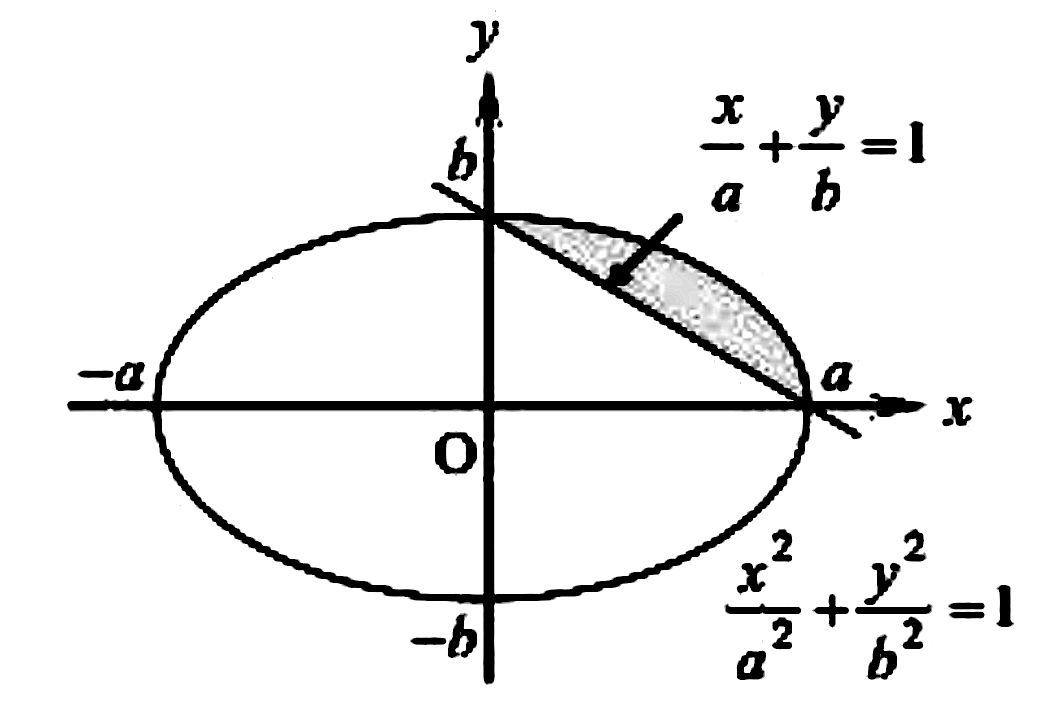
\includegraphics[width=0.35\textwidth]{28-28.4-24.png}
            \end{center}
            \begin{enumerate}
                  \item find $V_x$ and $V_y$. \sol{} \vspace{-0.8cm}
                        \begin{multicols}{2}
                              \begin{flalign*}
                                    V_x & = \pi \int_{0}^{a} \left\{ b^2\left(1 - \frac{x^2}{a^2}\right) - \left[b\left(1 - \dfrac{x}{a}\right)\right]^2\right\} dx & \\
                                        & = b^2 \pi \int_{0}^{a} \left( 1 - \frac{x^2}{a^2} - 1 + \frac{2x}{a} - \frac{x^2}{a^2} \right) dx                         & \\
                                        & = b^2 \pi \int_{0}^{a} \left( \frac{2x}{a} - \frac{2x^2}{a^2} \right) dx                                                  & \\
                                        & = b^2 \pi \left[ \frac{x^2}{a} - \frac{2x^3}{3a^2} \right]_{0}^{a}                                                        & \\
                                        & = b^2 \pi \left( \frac{a^2}{a} - \frac{2a^3}{3a^2} \right) = \frac{\pi ab^2}{3}
                              \end{flalign*}
                              \vfill\null
                              \begin{flalign*}
                                    V_y & = \pi \int_{0}^{b} \left\{ a^2\left(1 - \frac{y^2}{b^2}\right) - \left[a\left(1 - \dfrac{y}{b}\right)\right]^2\right\} dy & \\
                                        & = a^2 \pi \int_{0}^{b} \left( 1 - \frac{y^2}{b^2} - 1 + \frac{2y}{b} - \frac{y^2}{b^2} \right) dy                         & \\
                                        & = a^2 \pi \int_{0}^{b} \left( \frac{2y}{b} - \frac{2y^2}{b^2} \right) dy                                                  & \\
                                        & = a^2 \pi \left[ \frac{y^2}{b} - \frac{2y^3}{3b^2} \right]_{0}^{b}                                                        & \\
                                        & = a^2 \pi \left( \frac{b^2}{b} - \frac{2b^3}{3b^2} \right)  = \frac{\pi a^2b}{3}
                              \end{flalign*}
                              \vfill\null
                        \end{multicols}
                        \vspace{-1cm}

                  \item if $V_x = 2V_y$, find the value of $a:b$. \sol{}
                        \begin{flalign*}
                              \frac{\pi ab^2}{3} & = 2 \cdot \frac{\pi a^2b}{3} & \\
                              b                  & = 2a                         & \\
                              a:b                & = 1:2
                        \end{flalign*}
            \end{enumerate}
\end{enumerate}

\section{Revision Exercise 28}

\begin{enumerate}
    \item $\displaystyle\int_0^a\left(2 x^2-3 x+2\right) d x$
    \item $\displaystyle\int_1^3\left(x^2+\dfrac{1}{x^3}\right) d x$
    \item $\displaystyle\int_{-\dfrac{\pi}{6}}^{\frac{\pi}{2}}(3 \sin \theta-2 \cos 2 \theta) d \theta$
    \item $\displaystyle\int_{-\dfrac{\pi}{4}}^{\frac{\pi}{4}}\left(3 \sec ^2 \theta+\tan ^2 \theta\right) d \theta$
    \item $\displaystyle\int_0^{\ln 2} e^{3 x} d x$
    \item $\displaystyle\int_1^3 \dfrac{2}{3 x-1} d x$
    \item $\displaystyle\int_1^{16} \dfrac{2 x+3}{\sqrt{x}} d x$
    \item $\displaystyle\int_1^4 \dfrac{(\sqrt{x}-1)^2}{x} d x$
    \item $\displaystyle\int_1^2\left(x+\dfrac{4}{x^2}\right)^2 d x$
    \item $\displaystyle\int_0^1 \dfrac{x+1}{x^2+2 x+3} d x$
    \item $\displaystyle\int_{-1}^2 \dfrac{5 x}{\left(1+x^2\right)^4} d x$
    \item $\displaystyle\int_0^2 \dfrac{x}{\sqrt{25-4 x^2}} d x$
    \item $\displaystyle\int_2^4 \dfrac{3 x-2}{(2 x-3)^2} d x$
    \item $\displaystyle\int_2^4 \dfrac{2}{x^3-x} d x$
    \item $\displaystyle\int_1^3 \dfrac{1}{x^3+2 x^2+x} d x$
    \item $\displaystyle\int_0^\pi(\sin \theta+\cos \theta)^2 d \theta$
    \item $\displaystyle\int_0^{\frac{\pi}{3}} \sec ^2 \theta \tan \theta d \theta$
    \item $\displaystyle\int_{-\dfrac{\pi}{2}}^{\frac{\pi}{2}} \sin ^2 \theta \cos \theta d \theta$
    \item $\displaystyle\int_0^1 \dfrac{e^x}{e^x+1} d x$
    \item $\displaystyle\int_{\dfrac{\pi}{6}}^{\frac{\pi}{3}} \dfrac{\sec ^2 \theta}{\tan \theta} d \theta$
    \item Given that $\displaystyle\int_0^4 f(x) d x=2, \displaystyle\int_0^3 g(x) d
              x=4$, and $\displaystyle\int_3^8 g(x) d x=12$. Find the value of
          $\displaystyle\int_0^8\left[f\left(\dfrac{x}{2}\right)-2 g(x)\right] d x$.
    \item Given the function $y=(x+3) \sqrt{2 x-3}$, find $\dfrac{d y}{d x}$. Hence, find
          $\int_2^6 \dfrac{x}{\sqrt{2 x-3}} d x$.
    \item Given the function $y=x \ln x$, find $\dfrac{d y}{d x}$. Hence, find the
          following definite integrals:
          \begin{enumerate}
              \item $\displaystyle\int_1^4 \ln x d x$
              \item $\displaystyle\int_1^4 \ln (2 x) d x$
          \end{enumerate}
    \item Find the area of the region bounded by the curve $y=\dfrac{1}{x+1}$, the lines
          $x=1, x=7$, and the $x$-axis.
    \item Find the area of the region bounded by the curve $y=\dfrac{3}{x}$ and the line
          $y=4-x$.
    \item Find the area of the region bounded by the curve $x=y^2-5 y$ and the line $x+7
              y=24$.
    \item Find the area of the region bounded by the curves $y=x^2$ 及 $y^3=x$.
    \item Shown in the diagram below is the shaded region bounded by the curves $y=\ln x,
              y=\ln (2 x-1)$, and the line $y=3$. Find the area of this region.
    \item Find the area of the region bounded by the curves $x=y^3-y$ 及 $x=y-y^2$.
    \item Shown in the diagram below is the shaded region bounded by the curves $y=\sin
              x$ 及 $y=\sin 2 x$ in the interval $0 \leq x \leq \pi$. Find the area of this
          region.
    \item Find the volume of the solid of revolution formed by rotating the region
          bounded by the curve $y=\frac{1}{x+2}$, the line $x=2$, and two axes about the
          $x$-axis.
    \item Find the volume of the solid of revolution formed by rotating the region
          bounded by the curve $y=e^x-3$ and the two axes about the $x$-axis.
    \item Find the volume of the solid of revolution formed by rotating the region
          bounded by the curve $x=y^2-3 y$ and the $y$-axis about the $y$-axis.
    \item Find the volume of the solid of revolution formed by rotating the region
          bounded by the curve $y=x^2$ and the line $y=x+2$ about the $x$-axis.
    \item Find the volume of the solid of revolution formed by rotating the region
          bounded by the curve $y^2=x+9$ and the line $y=x+3$ about the $y$-axis.
    \item Given that a region is bounded by the curve $y^2=8 x$ and $y=x^2$. Find the
          volume of the solid of revolution formed by rotating this region about the
          $x$-axis and the $y$-axis respectively.
    \item SHown in the diagram below is the shaded region bounded by the curve $y =
              2\cos\pi x$, the line $y = 3x$, and the $y$-axis.
          \begin{enumerate}
              \item Prove that the $x$-coordinate of point $A$ is $\dfrac{1}{3}$.
              \item Find the volume of the solid of revolution formed by rotating this region about
                    the $x$-axis.
          \end{enumerate}
    \item Given that a region is bounded by the curve $xy = 12$, the line $x = 4$, and $y
              = 6$. Find the volume of the solid of revolution formed by rotating this region
          about the $x$-axis and the $y$-axis respectively.
\end{enumerate}

\end{document}